\documentclass[10pt]{article}

% basic packages
\usepackage[margin=1in]{geometry}
\usepackage{fix-cm}        % scale one design size, as OT1 does --- keeps the title bold
\usepackage[T1]{fontenc}   % accented French terms kept inline in the prose
\usepackage[pdftex]{graphicx}
\graphicspath{{./src/}}
\usepackage{amsmath,amssymb,amsthm}
\usepackage{custom}
\usepackage{pdfpages}
\usepackage{subcaption}
\usepackage{tabularx}
\usepackage{xcolor}

\usepackage{pgfplots}
\pgfplotsset{compat=1.15}
\usetikzlibrary{arrows,calc,decorations.markings,decorations.pathreplacing,patterns}

\renewcommand\qedsymbol{$\blacksquare$}

% page formatting
\usepackage{fancyhdr}
\pagestyle{fancy}

\usepackage{titlesec}
\titleformat*{\subsubsection}{\large\bfseries\sffamily}

\renewcommand{\sectionmark}[1]{\markright{\textsf{\arabic{section}. #1}}}
\renewcommand{\subsectionmark}[1]{}
\lhead{\textbf{\thepage} \ \ \nouppercase{\rightmark}}
\chead{}
\rhead{}
\lfoot{}
\cfoot{}
\rfoot{}
\setlength{\headheight}{14pt}

\linespread{1.03} % give a little extra room
\setlength{\parindent}{0in} % reduce paragraph indent a bit
\setcounter{secnumdepth}{2} % no numbered subsubsections
\setcounter{tocdepth}{2} % no subsubsections in ToC

\begin{document}

% make title page
\thispagestyle{empty}
\bigskip \
\vspace{0.1cm}

\begin{center}
{\fontsize{30}{30} \selectfont \bf \sffamily PHY 3TC20: Optique et Photonique }\\
\vspace{24pt}
%{\fontsize{14}{14} \selectfont \rmfamily Donald Kong} \\
%\vspace{6pt}
%{\fontsize{12}{12} \selectfont \ttfamily dkkl1137@gmail.com} \\
%\vspace{24pt}
\end{center}

{\parindent0pt \baselineskip=15.5pt
  This module is an introduction to optics. Over the last decades optics, until
  then a classical discipline, has developed very strong links with the
  information and communication sciences --- links that rest not only on a
  shared formalism (Fourier analysis) but also on the ability of optical waves
  to carry and store spatial signals naturally suited to parallel processing of
  the information they transport. The course gives the fundamental concepts of
  the discipline: propagation of light in optical fibres and the notion of
  transverse mode, by both a geometrical and a wave approach; lasers, and the
  difference between the mechanisms of light emission (thermal field,
  luminescence, stimulated emission); diffraction in scalar theory, Fourier
  optics and optical information processing --- spatial-frequency filtering,
  optical transfer functions, image sampling; and an introduction to
  holography, analogue and digital.

  \medskip
  Prose is in English; the French terms the poly, the TDs and the exam actually
  use are kept inline, so the vocabulary stays findable in both languages.
}

% make table of contents
% \newpage
\microtoc%
\newpage

% main content
\section{Optique géométrique et interférences}

L'\textbf{optique géométrique} (\textit{geometrical optics}) est élémentaire et
permet d'étudier les phénomènes lumineux lorsque tous les objets qui
interagissent avec la lumière ont des tailles caractéristiques grandes devant la
longueur d'onde du rayon lumineux. Nous verrons qu'elle a des limites et ne
permet donc pas d'expliquer certains phénomènes lumineux comme la diffraction ou
les interférences. Les lois générales d'optique géométrique peuvent être déduites
des équations de Maxwell et du \textbf{principe de Fermat}
(\textit{Fermat's principle}) --- la lumière se propage d'un point à un autre sur
des trajectoires telles que la durée du parcours soit stationnaire, que l'on
pourra comprendre, pour simplifier, par \emph{minimale}. Il est également
possible --- et c'est la méthode qui sera en partie choisie ici --- de poser ces
lois générales comme l'on poserait des axiomes, des expériences simples venant
les valider.\\

Ce chapitre est considéré comme un prérequis. It is not lectured in this course,
and the interference material collected in the second half is a prerequisite in
exactly the same sense.

\subsection{Principes fondamentaux}

\subsubsection{Indice de réfraction}

\begin{definition}[Indice de réfraction]
  Localement, l'\textbf{indice de réfraction} (\textit{refractive index}) $n$
  d'un milieu est le rapport de la vitesse de la lumière dans le vide $c$ sur la
  vitesse de la lumière $v$ dans le milieu considéré infini, isotrope et
  permanent :
  \[ n = \frac{c}{v}. \]
\end{definition}

L'indice caractérise en quelque sorte le ralentissement de la lumière par
rapport à sa vitesse dans le vide, $c \simeq 3\cdot 10^{8}\ \mathrm{m/s}$ : c'est
le \textbf{facteur de ralentissement} (\textit{slowing-down factor}) de la
lumière. La vitesse de la lumière dans le vide, appelée également
\textbf{célérité} (\textit{celerity}), est la vitesse maximale de la lumière :
$v \le c$. L'indice est donc toujours supérieur ou égal à 1 :

\[ n \ge 1 \quad \text{for every medium.} \]

Comme nous le verrons plus tard, l'indice dépend de la longueur d'onde du rayon
lumineux considéré.

\begin{center}
  \begin{tabular}{ll}
    \toprule
    Milieu & Indice \\
    \midrule
    vide                              & $n = 1$ \\
    air (20\textdegree C, 1 atm)      & $n = 1{,}000292$ \\
    eau                               & $n = 1{,}33$ \\
    verres                            & $n = 1{,}4$ à $1{,}9$ \\
    diamant                           & $n = 2{,}4$ \\
    germanium (semi-cond)             & $n \sim 4$ \\
    \bottomrule
  \end{tabular}
\end{center}

\subsubsection{Chemin optique d'un rayon lumineux le long d'une courbe quelconque et temps de parcours}

Suivant la valeur de l'indice de réfraction, la vitesse de la lumière varie.
Ainsi, pour une longueur \emph{physique} donnée d'un milieu traversé, le temps de
propagation ne sera pas identique. La notion de longueur physique en optique
n'est donc pas suffisante. On préférera utiliser la notion de
\textbf{chemin optique} (\textit{optical path}), qui pondère la longueur physique
par l'indice de réfraction.

\begin{definition}[Chemin optique]
  Localement, entre deux points voisins distants de $ds$, sur une courbe
  quelconque $C$, le chemin optique est défini par $dL = n\,ds$, $n$ étant
  l'indice optique du milieu au point considéré. Le chemin optique entre deux
  points $A$ et $B$ de cette courbe est par définition l'intégrale curviligne le
  long de la trajectoire considérée :
  \[ L_{\text{optique}}(AB) = \int_{AB} n\, ds. \]
  $n$ n'est ici pas forcément une constante et varie le long de $C$.
\end{definition}

Un milieu homogène, infini, permanent et isotrope est caractérisé par un indice
optique uniforme. Si on reprend l'expression du chemin optique, celle-ci devient

\[ L_{\text{optique}}(AB) = \int_{AB} n\, ds = n\, L_{\text{physique}}. \]

Le temps de parcours suivant une trajectoire de longueur $L_{\text{physique}}$
est alors

\[ t = \frac{L_{\text{physique}}}{v}
     = \frac{n\, L_{\text{physique}}}{c}
     = \frac{L_{\text{optique}}}{c}. \]

\begin{remark}
  The \emph{chemin optique} is divided by $c$, not by $v$: dividing it by $v$
  would introduce $n^{2}$. Every member holds; the last two,
  $t = n L_{\text{physique}}/c = L_{\text{optique}}/c$, show that the chemin optique is
  precisely the distance light would have covered \emph{in vacuum} in the same
  time.
\end{remark}

\subsubsection{Propagation rectiligne dans un milieu homogène, infini, permanent et isotrope}

\begin{postulate}[Propagation rectiligne (\textit{rectilinear propagation})]
  Dans un milieu homogène, l'indice $n$ est constant et la lumière se propage en
  ligne droite.
\end{postulate}

This follows directly from the expression above, with $n$ constant. Il en résulte
que $L_{\text{optique}}$ est minimal si $AB$ s'identifie à une droite. The
Fermat-stationary trajectory is therefore the straight line. Un exemple de milieu
homogène est le vide ou l'air si la température et la pression sont constantes.\\

Two experiments make the principle visible, the first with a mask in front of a
source. Les phénomènes d'ombres et de pénombres s'expliquent aisément à partir du
principe de propagation rectiligne. De même, un faisceau laser (HeNe par
exemple), matérialisé par la diffusion de particules de fumée, donne une idée de
la propagation rectiligne.

\begin{example}[Transit time over 100\,km]
  Calculer le temps de propagation de la lumière pour un chemin physique de
  $100$\,km dans l'air puis dans une fibre en verre pour des longueurs d'onde de
  $\lambda = 0{,}6\ \mu$m. Refaire ces calculs pour la longueur d'onde Télécom de
  $\lambda = 1{,}55\ \mu$m.\\

  With $L_{\text{physique}} = 10^{5}$\,m and $c \simeq 3\cdot 10^{8}$\,m/s the
  vacuum transit is $L/c = 333{,}3\ \mu$s. In air, $n = 1{,}000292$ gives
  \[ t_{\text{air}} = \frac{n L}{c} = 1{,}000292 \times 333{,}3\ \mu\mathrm{s}
     \simeq 333{,}4\ \mu\mathrm{s}, \]
  i.e.\ only about $0{,}1\ \mu$s more than in vacuum. In a glass, the table of
  indices above gives $n = 1{,}4$ to $1{,}9$; taking a representative
  $n = 1{,}5$,
  \[ t_{\text{verre}} = 1{,}5 \times 333{,}3\ \mu\mathrm{s} = 500\ \mu\mathrm{s}. \]
  The point of the second question is that $n = n(\lambda)$: the same $100$\,km
  of the same fibre is not crossed in the same time at $0{,}6\ \mu$m and at
  $1{,}55\ \mu$m, and evaluating the difference requires the dispersion curve of
  the glass, which is not tabulated here. The order of magnitude worth carrying
  away is that a fibre link costs roughly $5\ \mu$s of latency per kilometre,
  about half again the free-space figure.
\end{example}

\subsubsection{Principe d'indépendance des faisceaux lumineux}

\begin{postulate}[Indépendance des faisceaux lumineux (\textit{independence of light beams})]
  Les rayons lumineux traversant un même milieu sont indépendants les uns des
  autres.
\end{postulate}

Cela se traduit de deux façons. D'une part, dans un faisceau de rayons lumineux,
l'action sur certains rayons (arrêt, déviation, \dots) n'a aucun effet sur les
autres : l'éclairement de l'écran au-dessus du point $A$ reste inchangé quand on
intercepte une partie du faisceau, $E_1 = E_2$. D'autre part, quand deux
faisceaux se croisent, il n'y a pas d'interaction : il en est de même,
$E'_1 = E'_2$, après que l'on ait fait se croiser les faisceaux I et II.

\begin{remark}[Limits of the two preceding principles]
  Une observation très précise de la frontière séparant la lumière de l'ombre
  montre des variations d'éclairement qui ne peuvent être expliquées par les deux
  principes de propagation rectiligne et d'indépendance des rayons. Seule la
  théorie ondulatoire de la lumière permet de préciser ce phénomène
  d'éparpillement, ce qui sera vu par la suite au chapitre « diffraction ».
\end{remark}

\begin{remark}[What about interference?]
  Les interférences ne se produisent qu'en présence d'un détecteur, qui effectue
  le module au carré de la \emph{somme} des champs. Pas de détecteur, pas
  d'interférence, même quand les faisceaux se croisent. The principe
  d'indépendance des faisceaux lumineux is a statement about the fields, not
  about what a \textbf{détecteur quadratique} (\textit{square-law detector})
  reports.
\end{remark}

\subsubsection{Principe du retour inverse}

\begin{postulate}[Principe du retour inverse (\textit{inverse return})]
  Dans les milieux transparents, le trajet effectivement suivi par la lumière
  d'un point $A$ vers un point $B$ (resp.\ de $B$ vers $A$) est indépendant du
  sens de parcours.
\end{postulate}

Ce principe est valable même dans les milieux hétérogènes où le trajet est
courbe, comme nous le montrerons plus tard dans le chapitre « fibre optique ».
Une \textbf{autocollimation} réalisée avec un faisceau laser sur un miroir plan
montre la validité du principe du retour inverse. Un \textit{collimateur} est un
dispositif optique permettant d'obtenir un faisceau de rayons de lumière
parallèles à partir d'une source de lumière. Ce mot vient du latin
\textit{collimatio} (« ajuster ou viser en ligne droite »).

\subsection{Réflexion et réfraction, loi de Descartes-Snell}

\begin{definition}[Dioptre]
  Un \textbf{dioptre} (\textit{refracting interface}) est une surface séparant
  deux milieux transparents d'indices de réfraction différents, par exemple la
  surface entre l'air et l'eau.
\end{definition}

\begin{definition}[Réfraction]
  Si la lumière se propage en ligne droite dans un milieu homogène et isotrope
  (invariant par rotation), elle est déviée lors de la traversée d'un dioptre :
  c'est le phénomène de \textbf{réfraction}.
\end{definition}

\subsubsection{Lois de Descartes-Snell}

Ces lois ont été trouvées par W.~Snell en 1621 et retrouvées par R.~Descartes en
1636 --- la première mention de la loi de la réfraction a été faite par Ibn Sahl
autour de 984. Elles permettent de connaître le changement de direction, par
réflexion ou par réfraction, d'un rayon lumineux rectiligne, à la traversée d'une
surface (dioptre) séparant deux milieux homogènes. Ces lois sont au nombre de 3.

\begin{theorem}[Lois de Descartes-Snell (\textit{Descartes--Snell laws})]
  \begin{subpart}
    \item Les rayons incident, réfléchi, réfracté et la normale au point
      d'incidence à la surface du dioptre sont \textbf{coplanaires}.
    \item Le rayon réfléchi est symétrique du rayon incident par rapport à la
      normale au point d'incidence :
      \[ i = -r. \]
    \item Les sinus des angles de réfraction et d'incidence sont dans un rapport
      constant :
      \[ n \sin i = n' \sin i'. \]
  \end{subpart}
\end{theorem}

\begin{notation}
  Angles are measured from the normal to the dioptre. $n$ and $i$ are the index
  and the angle on the incidence side, $n'$ and $i'$ the index and the angle on
  the transmission side, $r$ the reflection angle. The reflection law is written
  $i = -r$ (signed angles, measured on either side of the normal), which in
  magnitude is $i = r$.
\end{notation}

\begin{figure}[h!]
  \centering
  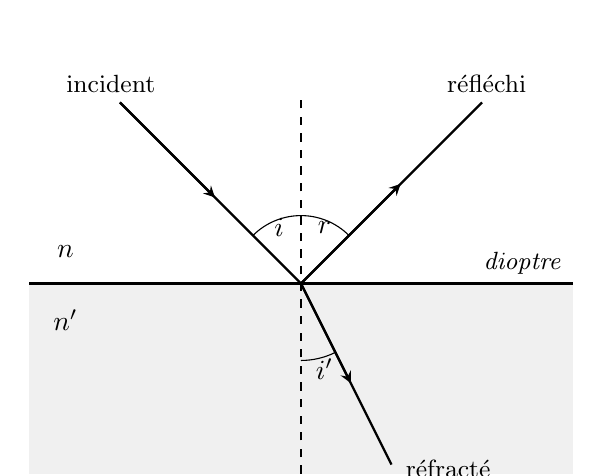
\begin{tikzpicture}[>=stealth,scale=1.15]
    \fill[gray!12] (-3.0,-2.1) rectangle (3.0,0);
    \draw[very thick] (-3.0,0) -- (3.0,0);
    \draw[dashed] (0,-2.1) -- (0,2.1);
    % incident
    \draw[thick] (-2.0,2.0) -- (0,0);
    \draw[->,thick] (-2.0,2.0) -- (-0.95,0.95);
    % reflected
    \draw[thick] (0,0) -- (2.0,2.0);
    \draw[->,thick] (0,0) -- (1.1,1.1);
    % refracted
    \draw[thick] (0,0) -- (1.0,-2.0);
    \draw[->,thick] (0,0) -- (0.55,-1.1);
    % angle arcs
    \draw (0,0.75) arc (90:135:0.75);
    \node at (-0.24,0.62) {$i$};
    \draw (0,0.75) arc (90:45:0.75);
    \node at (0.26,0.62) {$r$};
    \draw (0,-0.85) arc (270:296.5:0.85);
    \node at (0.26,-0.95) {$i'$};
    \node at (-2.6,0.35) {$n$};
    \node at (-2.6,-0.4) {$n'$};
    \node at (2.05,2.2) {\small réfléchi};
    \node at (-2.1,2.2) {\small incident};
    \node[right] at (1.05,-2.05) {\small réfracté};
    \node[rotate=0] at (2.45,0.22) {\small \textit{dioptre}};
  \end{tikzpicture}

  \smallskip
  {\small\itshape The three lois de Descartes-Snell at a dioptre: coplanarity,
  $i=-r$, $n \sin i = n' \sin i'$.}
\end{figure}

\begin{example}[The broken stick (le bâton brisé)]
  La loi de la réfraction explique pourquoi, lorsque l'on trempe une partie d'un
  bâton dans l'eau, on a l'impression que celui-ci est cassé. L'extrémité du
  bâton émet des rayons lumineux dans toutes les directions et seuls quelques
  rayons vont parvenir à notre œil. Mais ceux-ci sont réfractés et se sont
  \emph{éloignés} par rapport à la normale en changeant de milieu eau-air pour
  parvenir à l'œil. Cette réfraction n'est pas perçue par l'œil qui construit
  l'image de la partie immergée du bâton en suivant les rayons virtuels :
  l'extrémité du bâton parait donc à un autre endroit qu'il ne l'est réellement.
\end{example}

\subsubsection{Dispersion}

La vitesse de propagation de la lumière dans un milieu matériel dépend de la
longueur d'onde ($\equiv$ la couleur). Cette dépendance de $v$ avec $\lambda$
s'appelle la \textbf{dispersion chromatique} (\textit{chromatic dispersion}). Il
en est donc de même pour l'indice :

\[ v = v(\lambda), \qquad n = n(\lambda). \]

La dispersion du vide est nulle et la dispersion de l'air est négligeable. For
most purposes, then,

\[ n_{\text{vide}} = 1 \simeq n_{\text{air}}. \]

\subsubsection{Angle limite et réflexion totale}

D'après la loi de la réfraction, $n \sin i = n' \sin i'$. That is,
$\sin i' = (n/n') \sin i$. Or, on sait que $-1 \le \sin i \le 1$. The bound is on
the \emph{incidence} angle. Donc

\[ -\frac{n}{n'} \le \sin i' \le \frac{n}{n'} , \]

et suivant la valeur relative de $n$ par rapport à $n'$, deux cas se présentent.
\textbf{Réfringent} : qui cause une réfraction de la lumière. Plus le milieu est
réfringent, plus l'indice de réfraction est élevé.

\begin{subpart}
  \item $n' > n$ : le faisceau passe alors d'un milieu moins réfringent à un
    milieu plus réfringent (de l'air vers l'eau par exemple). Le rayon se
    \emph{rapproche} alors systématiquement de la normale, $i' < i$, il est donc
    toujours réfracté. Il n'y a pas d'angle limite.
  \item $n' < n$ : le faisceau passe alors d'un milieu plus réfringent à un
    milieu moins réfringent (de l'eau vers l'air). Le rayon réfracté
    s'\emph{écarte} de la normale, $i' > i$. Dans ce cas, il existe un
    \textbf{angle limite} (\textit{critical angle}) $i = i_c$ pour lequel
    l'angle de réfraction est égal à $90$\textdegree. Lorsque $i$ devient supérieur, l'expérience montre qu'il
    n'existe plus de lumière réfractée et donc transmise : il y a
    \textbf{réflexion totale} (\textit{total reflection}).
\end{subpart}

\begin{theorem}[Angle limite (ou angle critique)]
  Si $n' < n$, il existe un angle limite $i_c$,
  \[ \boxed{\ \sin i_c = \frac{n'}{n}\ } \]
  et si $i > i_c$, pas de faisceau réfracté : réflexion totale de la lumière.
\end{theorem}

\begin{figure}[h!]
  \centering
  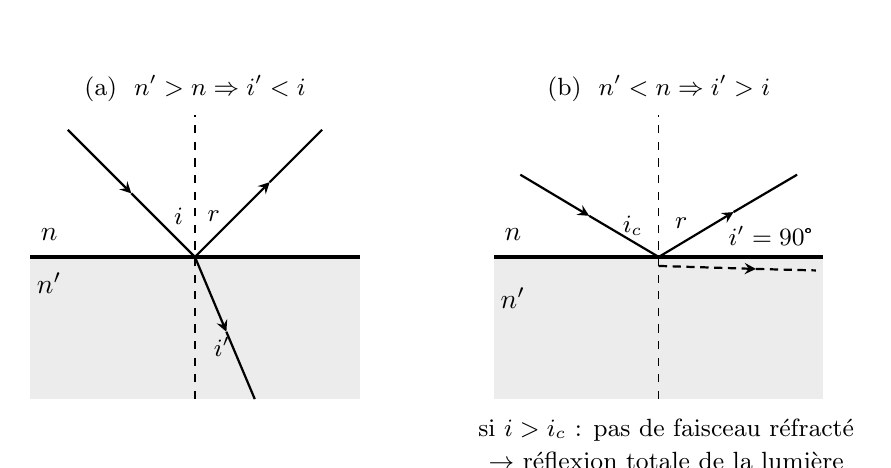
\begin{tikzpicture}[>=stealth,scale=0.95]
    % ---- panel a : n' > n ----
    \begin{scope}[shift={(0,0)}]
      \fill[gray!15] (-2.2,-1.9) rectangle (2.2,0);
      \draw[very thick] (-2.2,0) -- (2.2,0);
      \draw[dashed] (0,-1.9) -- (0,1.9);
      \draw[->,thick] (-1.7,1.7) -- (-0.85,0.85);
      \draw[thick] (-0.85,0.85) -- (0,0);
      \draw[->,thick] (0,0) -- (1.0,1.0);
      \draw[thick] (1.0,1.0) -- (1.7,1.7);
      \draw[->,thick] (0,0) -- (0.42,-1.0);
      \draw[thick] (0.42,-1.0) -- (0.8,-1.9);
      \node at (-0.22,0.55) {\small $i$};
      \node at (0.25,0.55) {\small $r$};
      \node at (0.36,-1.2) {\small $i'$};
      \node at (-1.95,0.3) {$n$};
      \node at (-1.95,-0.35) {$n'$};
      \node at (0,2.25) {\small (a)\ \ $n' > n \Rightarrow i' < i$};
    \end{scope}
    % ---- panel b : n' < n ----
    \begin{scope}[shift={(6.2,0)}]
      \fill[gray!15] (-2.2,-1.9) rectangle (2.2,0);
      \draw[very thick] (-2.2,0) -- (2.2,0);
      \draw[dashed] (0,-1.9) -- (0,1.9);
      \draw[->,thick] (-1.85,1.1) -- (-0.93,0.55);
      \draw[thick] (-0.93,0.55) -- (0,0);
      \draw[->,thick] (0,0) -- (1.0,0.6);
      \draw[thick] (1.0,0.6) -- (1.85,1.1);
      \draw[->,thick,densely dashed] (0,-0.12) -- (1.3,-0.16);
      \draw[thick,densely dashed] (1.3,-0.16) -- (2.1,-0.18);
      \node at (-0.35,0.42) {\small $i_c$};
      \node at (0.3,0.45) {\small $r$};
      \node at (1.5,0.28) {\small $i'=90$\textdegree};
      \node at (-1.95,0.3) {$n$};
      \node at (-1.95,-0.55) {$n'$};
      \node at (0,2.25) {\small (b)\ \ $n' < n \Rightarrow i' > i$};
      \node[align=center] at (0.1,-2.5)
        {\small si $i>i_c$ : pas de faisceau réfracté\\ \small $\rightarrow$ réflexion totale de la lumière};
    \end{scope}
  \end{tikzpicture}

  \smallskip
  {\small\itshape Réfraction en fonction de $n$, $n'$ et de l'angle d'incidence.
  An angle limite exists only in case (b).}
\end{figure}

Two everyday observations bracket the two cases. Chacun a déjà regardé la
surface de l'eau sur le bord d'une piscine. Il a constaté que, lorsque la surface
de l'eau est plane, quel que soit l'angle sous lequel il regarde l'eau, malgré
les reflets, il pourra voir le fond de la piscine (air to water: no angle
limite). À l'inverse, lorsque l'on fait de la plongée, si l'on essaye
de regarder la surface de l'eau avec un angle rasant, on ne voit pas du tout le
ciel, on observe au contraire un miroir parfait. Au-delà d'un certain angle
appelé angle limite, $i_c$, il y a réflexion totale.

\begin{remark}
  Comme nous le verrons plus tard, c'est l'existence d'un angle limite qui permet
  de guider la lumière dans une fibre optique par réflexion totale interne.
\end{remark}

\begin{example}[The aquarium]
  On remplit un aquarium d'eau. On éclaire la surface de l'eau avec un laser
  rouge, $\lambda = 0{,}6\ \mu$m. Take $n = 1{,}33$ for the water and
  $n_{\text{air}} = 1$.
  \begin{subpart}
    \item On oriente le laser perpendiculairement à l'eau. L'angle d'incidence se
      mesure par rapport à la normale à la surface de séparation entre les deux
      milieux (dioptre). Donc, $i = 0$\textdegree.
    \item Angle de réfraction : $\sin i' = (n/n')\sin i = 0$, so
      $i' = 0$\textdegree{} --- a ray at normal incidence is not deviated.
    \item On éclaire maintenant la surface de l'eau avec une incidence
      $i = 45$\textdegree. L'angle de réflexion est toujours identique à l'angle
      d'incidence, c'est-à-dire $r = 45$\textdegree. For the refraction,
      \[ \sin i' = \frac{n_{\text{air}}}{n_{\text{eau}}}\sin 45^{\circ}
                 = \frac{0{,}707}{1{,}33} = 0{,}532
         \quad\Longrightarrow\quad i' \simeq 32^{\circ}, \]
      the ray bending towards the normal as expected for $n' > n$.
    \item Angle limite de l'air vers l'eau. There is none: here $n' > n$, the
      refracted ray always exists; this is case (a) above and the expected answer
      is that the question has no solution.
    \item Angle limite de l'eau vers l'air :
      \[ \sin i_c = \frac{n_{\text{air}}}{n_{\text{eau}}} = \frac{1}{1{,}33}
         = 0{,}752 \quad\Longrightarrow\quad i_c \simeq 48{,}8^{\circ}. \]
  \end{subpart}
\end{example}

\subsubsection{Formules de Fresnel}

The lois de Descartes-Snell fix the \emph{directions}; the
\textbf{formules de Fresnel} (\textit{Fresnel formulas}) fix the
\emph{amplitudes}. Decomposing the incident field into a component
$E_{\parallel}$ in the plane of incidence and a component $E_{\perp}$
perpendicular to it, the amplitude reflection and transmission coefficients at a
dioptre $n_1/n_2$ are

\[ r_{\parallel} = -\frac{\tan(i-i')}{\tan(i+i')}, \qquad
   r_{\perp}     = -\frac{\sin(i-i')}{\sin(i+i')}, \]
\[ t_{\parallel} = \frac{2\cos i \sin i'}{\sin(i+i')\cos(i-i')}, \qquad
   t_{\perp}     = \frac{2\cos i \sin i'}{\sin(i+i')}. \]

\begin{remark}[Déphasage à la réflexion]
  Le \textbf{déphasage à la réflexion} (\textit{phase shift on reflection}) vaut
  $\pi$ (signe (-) de $r_{\parallel}$ et $r_{\perp}$) tant que l'on ne se trouve
  pas en réflexion totale. Dans le cas de la réflexion totale, ce déphasage est
  beaucoup plus compliqué et dépend à la fois de la polarisation et de l'angle
  d'incidence. Phénomène important dans la fibre optique.
\end{remark}

Dans le cas d'une incidence normale, on admet que le coefficient de réflexion en
amplitude sur un dioptre séparant 2 milieux d'indices $n_1$ et $n_2$ vaut

\[ r = \frac{n_2 - n_1}{n_2 + n_1}, \]

the simplified form needed for the anti-reflection coating below.

\subsection{Interférences à deux ondes}

La théorie des interférences traite de la superposition de deux ou plusieurs
champs électriques, qu'ils soient mono ou polychromatiques. Les phénomènes
ondulatoires sont décrits par une équation différentielle du second ordre
(équation de Helmholtz) et par conséquent, le \textbf{principe de superposition}
(\textit{superposition principle}) s'applique. Il en résulte qu'en tout point où
deux ou plusieurs champs optiques se superposent, l'amplitude $\v{E}$ du champ
résultant est la \emph{somme vectorielle} des amplitudes de chaque composante.

\begin{definition}[Interférences]
  Deux faisceaux \textbf{interfèrent} lorsque l'intensité résultant de la
  superposition de ces ondes n'est \emph{pas} la somme de leur intensité.
\end{definition}

Des interférences facilement observables sont celles que l'on obtient en jetant
non pas un seul mais deux cailloux dans l'eau, à deux endroits différents. Si on
regarde les rides à la surface de l'eau, il y aura des régions où les ondes se
compenseront voire s'annuleront totalement et d'autres, par contre, où les creux
et les crêtes seront accentués. Ainsi, si l'on superpose deux faisceaux
lumineux, sous certaines conditions que nous expliciterons, il est possible
d'obtenir de l'obscurité. On peut donc créer de l'obscurité avec de la lumière et
écrire alors la simple formule « lumière + lumière = obscurité ».

\subsubsection{Étude intuitive}

Soit une vibration lumineuse $E_0$ que nous séparons en deux à l'aide d'un
miroir semi-réfléchissant. Faisons parcourir à ces deux ondes deux chemins $z_1$
et $z_2$, puis re-superposons ces deux ondes. Après recombinaison, suivant les
chemins parcourus, les deux ondes peuvent se retrouver ou non en phase.

\begin{subpart}
  \item Si elles sont en phase, $\Delta\phi = 2m\pi$ avec $m$ entier, la somme
    des champs redonne le champ initial, $\v{E}_1 + \v{E}_2 = \v{E}_0$, et
    $I = I_0$ : on parle alors d'\textbf{interférences constructives}
    (\textit{constructive interference}).
  \item Si au contraire elles sont en opposition de phase, c'est que l'une des
    deux ondes a accumulé $(2m+1)\pi$ de phase en plus de l'autre. On peut alors
    écrire
    \[ \v{E}_1 + \v{E}_2
       = \v{E}_1 \underbrace{e^{2im\pi}}_{=\,1}
         \bigl(1 + \underbrace{e^{i\pi}}_{=\,-1}\bigr) = 0 . \]
    Le champ électrique s'annule. Pas de champ électrique, pas de lumière : on
    parle alors d'\textbf{interférences destructives}
    (\textit{destructive interference}), $I = 0$.
\end{subpart}

Since the phase difference is set by the path lengths, this is already a way of
\emph{coding a distance} into an intensity.

\subsubsection{Étude générale}

Considérons deux ondes lumineuses issues de la même source, monochromatiques,
polarisées rectilignement. En notation complexe, elles s'écrivent

\[ \v{E}' = E_1 e^{2i\pi\nu t}\, \v{e}_1, \qquad
   \v{E}'' = E_2 e^{2i\pi\nu t}\, \v{e}_2, \qquad
   E_1 = A e^{-i\phi_1}, \quad E_2 = A e^{-i\phi_2}, \]

où $E_1, E_2$ sont les amplitudes complexes correspondantes, $\phi_1, \phi_2$ les
phases des vibrations et $\v{e}_1, \v{e}_2$ des vecteurs unitaires portant la
direction d'oscillation du champ électrique, c'est-à-dire la direction de
polarisation. These phases are spatial. Le champ électrique résultant de la
superposition de ces deux ondes est la somme des deux champs, puisque les
équations de Maxwell auxquelles ils doivent satisfaire sont linéaires :

\[ \v{E} = \v{E}' + \v{E}'' = \bigl(E_1 \v{e}_1 + E_2 \v{e}_2\bigr) e^{2i\pi\nu t}. \]

L'intensité simplifiée de l'onde résultante sur un détecteur quadratique est

\[ I = \varepsilon_0 c |\v{E}|^{2}
     = \varepsilon_0 c \,\bigl|\v{E}' + \v{E}''\bigr|^{2}
     \propto E_1 E_1^{*} + E_2 E_2^{*}
       + \v{e}_1 \cdot \v{e}_2 \,\bigl(E_1 E_2^{*} + E_1^{*} E_2\bigr), \]

soit, après simplifications,

\[ \boxed{\ I \simeq I_1 + I_2 + 2\,(\v{e}_1\cdot\v{e}_2)\sqrt{I_1 I_2}\,
   \cos\Delta\phi \ } \]

où $\Delta\phi = \phi_2 - \phi_1$ désigne le retard de phase de l'onde 2 par
rapport à l'onde 1 (notons que l'on aurait pu prendre l'opposé car le cosinus est
pair), et $\v{e}_1 \cdot \v{e}_2$ représente le produit scalaire entre les
vecteurs unitaires portant les directions de polarisation de chaque onde. Il vaut
$1$ si les deux polarisations sont coplanaires, il est nul si elles sont
perpendiculaires.

\begin{conclusion}
  Cette équation est la formule de base de tous les problèmes d'interférences à
  deux ondes.
\end{conclusion}

\begin{remark}[Crossed polarisations]
  Lorsque les polarisations sont perpendiculaires, $\v{e}_1 \cdot \v{e}_2 = 0$ et
  $I = I_1 + I_2$ : il n'y a plus d'interférence, l'intensité totale est la
  simple addition des deux intensités.
\end{remark}

\subsubsection{Cas particulier : ondes polarisées rectilignement, coplanaires, issues d'une même source}

À partir de maintenant, les champs seront considérés comme linéairement polarisés
et \emph{de surcroît} coplanaires. Le produit scalaire vaut alors $1$ et
l'approche, théoriquement vectorielle, se réduit à un problème scalaire :

\[ I \simeq \underbrace{I_1 + I_2}_{\text{addition des intensités}}
   + \underbrace{2\sqrt{I_1 I_2}\cos\Delta\phi}_{\text{terme d'interférence}} . \]

On constate que l'intensité totale est la somme des intensités de chaque onde et
d'un \textbf{terme d'interférence} (\textit{interference term}).

\paragraph{Notion de différence de marche.} La phase de chaque onde prend la
forme

\[ \phi_1 = \phi_{\text{origine}\,1} + \phi_{\text{accumulée}\,1}, \qquad
   \phi_2 = \phi_{\text{origine}\,2} + \phi_{\text{accumulée}\,2}. \]

Les deux ondes proviennent de la même source, donc la phase à l'origine est la
même pour les deux ondes : on parle alors d'ondes \textbf{cohérentes}. La phase à
l'origine s'annule donc dans l'expression de $\Delta\phi$ et on peut pour
simplifier la considérer comme nulle,
$\phi_{\text{origine}\,1} = \phi_{\text{origine}\,2} = \phi_{\text{origine}} = 0$.
La phase accumulée dépend du chemin optique parcouru par l'onde :

\[ \phi_{\text{accumulée}\,1} = \frac{2\pi n z_1}{\lambda}, \qquad
   \phi_{\text{accumulée}\,2} = \frac{2\pi n z_2}{\lambda}, \]

où $n$ est l'indice optique du milieu et $z_1, z_2$ les distances parcourues par
chaque onde depuis leur séparation. Here $\lambda$ is the longueur d'onde in
vacuum. (Pour simplifier, on considère que les deux ondes parcourent des milieux
de même indice de réfraction $n$. Ceci n'est bien sûr pas toujours le cas.) On
peut donc en déduire l'expression du déphasage :

\[ \Delta\phi = 2\pi\frac{n(z_2 - z_1)}{\lambda} = 2\pi\frac{\delta}{\lambda},
   \qquad \boxed{\ \delta = n(z_2 - z_1)\ } \]

\begin{definition}[Différence de marche]
  La \textbf{différence de marche} (\textit{path difference}) $\delta$
  correspond à la différence de chemins optiques parcourus par les deux ondes
  depuis leur séparation jusqu'à leur recombinaison. Dans un problème
  d'interférences, tout le travail est de calculer la différence de marche entre
  les deux ondes.
\end{definition}

\paragraph{Interférence à deux ondes en lumière cohérente.} $\Delta\phi$ est
indépendante du temps, $\cos\Delta\phi$ variant dans $[-1,+1]$ :

\begin{subpart}
  \item $\Delta\phi = \pm 2m\pi \Leftrightarrow \delta = \pm m\lambda
    \Rightarrow \cos\Delta\phi = 1$ : $I$ est maximale, interférences
    constructives.
  \item $\Delta\phi = \pm(2m+1)\pi \Leftrightarrow
    \delta = \pm(2m+1)\dfrac{\lambda}{2} \Rightarrow \cos\Delta\phi = -1$ :
    $I$ est minimale, interférences destructives.
\end{subpart}

$I$ oscille entre les deux valeurs extrêmes

\[ I_{\min} = \bigl(\sqrt{I_1} - \sqrt{I_2}\bigr)^{2}, \qquad
   I_{\max} = \bigl(\sqrt{I_1} + \sqrt{I_2}\bigr)^{2}. \]

Si les amplitudes de chaque onde sont égales, c'est-à-dire $E_1 = E_2 = E_0$,
l'expression se simplifie :

\[ I(\Delta\phi) \propto 2 I_0 \bigl(1 + \cos\Delta\phi\bigr), \qquad
   I(\delta) \propto 2 I_0 \left(1 + \cos\left(2\pi\frac{\delta}{\lambda}\right)\right), \]

et le contraste des franges est alors maximum :
$I_{\max} = 4 I_0$ et $I_{\min} = 0$.

\begin{remark}
  The preceding equation $I \propto 2I_0(1+\cos\Delta\phi)$ fixes the two
  labels: the maximum is $4I_0$, reached where $\cos\Delta\phi = 1$, and the
  minimum is $0$, reached where $\cos\Delta\phi = -1$.
\end{remark}

\begin{figure}[h!]
  \centering
  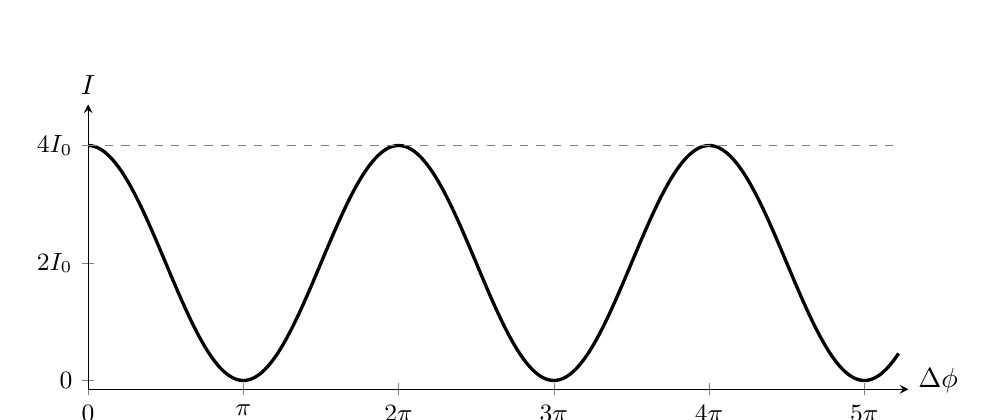
\begin{tikzpicture}
    \begin{axis}[
      width=12cm, height=5.2cm,
      axis lines=left,
      xmin=0, xmax=16.6, ymin=-0.15, ymax=4.7,
      xtick={0,3.14159,6.28319,9.42478,12.56637,15.70796},
      xticklabels={$0$,$\pi$,$2\pi$,$3\pi$,$4\pi$,$5\pi$},
      ytick={0,2,4},
      yticklabels={$0$,$2I_0$,$4I_0$},
      xlabel={$\Delta\phi$},
      ylabel={$I$},
      every axis x label/.style={at={(current axis.right of origin)},anchor=west},
      every axis y label/.style={at={(current axis.above origin)},anchor=south},
      tick label style={font=\small},
      ]
      \addplot[very thick,domain=0:16.4,samples=300,smooth]
        {2*(1+cos(deg(x)))};
      \draw[dashed,gray] (axis cs:0,4) -- (axis cs:16.4,4);
    \end{axis}
  \end{tikzpicture}

  \smallskip
  {\small\itshape Interférences à deux ondes en lumière monochromatique, si
  $I_1 = I_2 = I_0$. The same curve read against $\delta$ has its bright fringes
  at $\delta = 0, \lambda, 2\lambda, \dots$}
\end{figure}

\begin{definition}[Interfrange]
  On passe d'une frange brillante à la frange brillante suivante en faisant
  varier la différence de marche d'une longueur d'onde, soit $0{,}5\ \mu$m dans
  le jaune. On parle d'\textbf{interfrange} (\textit{fringe spacing}). The orders
  of magnitude at stake in a figure d'interférence are sub-micron.
\end{definition}

\subsection{Notion de cohérence}

Nous avons dans le cas précédent illustré la notion d'interférence à partir
d'une source unique, monochromatique, que nous avons séparée en deux puis
recombinée. Nous avons donc considéré que la phase à l'origine de l'émission
était commune aux deux ondes. Nous avons également considéré les ondes
parfaitement monochromatiques, donc avec des longueurs de \textbf{train d'onde}
(\textit{wave train}) infinies. En réalité, nous sommes à tout instant soumis à
la superposition de plusieurs ondes. Par exemple, lorsque j'allume la lumière
chez moi, je suis éclairé par les rayons issus directement de la source mais
également ceux réfléchis par les murs, le plafond. Pour autant, nous n'observons
pas de frange brillante ni sombre. Il existe donc des conditions auxquelles
doivent satisfaire deux faisceaux lumineux pour pouvoir interférer.

\subsubsection{Mécanisme d'émission par une source lumineuse}

Les ondes électromagnétiques ne sont pas émises de façon continue, mais tout se
passe comme si elles étaient émises par paquets provenant de divers atomes. Ces
atomes n'émettent pratiquement que pendant un temps limité $\tau$ qui correspond
à la durée de vie dans la théorie quantique et le coefficient d'amortissement en
théorie classique. This durée de vie is that of an excited state.\\

Si l'on attend un temps important par rapport à $\tau$, les vibrations observées
à l'instant initial auront disparu, d'autres atomes auront pris le relais, mais
les vibrations n'auront plus aucune relation avec les vibrations initiales, leur
amplitude et leur phase ayant changé. Le phénomène se reproduit un grand nombre
de fois par seconde. En d'autres termes, \emph{la phase à l'origine varie dans le
temps : elle est aléatoire}. Naturellement, cela est également vrai pour deux
vibrations émises par deux sources différentes : elles n'ont pas de relation de
phases entre elles, et la différence de phase entre les deux ondes varie
aléatoirement dans le temps.

\begin{remark}
  Tout le secret de l'émission laser réside principalement dans la mise en phase
  des différents trains d'onde successifs, comme nous le verrons plus tard dans
  le chapitre « laser ».
\end{remark}

\subsubsection{Conséquence d'une phase aléatoire dans le temps sur les interférences}

En pratique, l'intensité mesurée dépend du temps d'intégration $T_D$ du
détecteur, relié à la notion de bande passante par la formule $BP = 1/T_D$. Si la
différence de phase des deux ondes n'est pas constante dans le temps mais
aléatoire, c'est-à-dire que la lumière provient de deux sources différentes, on
ne peut pas sortir $\Delta\phi$ de la moyenne sur le temps, et l'expression de
l'intensité aurait dû s'écrire

\[ I \simeq I_1 + I_2 + 2\,(\v{e}_1\cdot\v{e}_2)\sqrt{I_1 I_2}\,
     \langle \cos\Delta\phi \rangle_{T_D},
   \qquad
   \langle \cos\Delta\phi \rangle_{T_D}
     = \frac{1}{T_D}\int_0^{T_D} \cos\Delta\phi \; dt . \]

Si de plus $\Delta\phi$ peut prendre n'importe quelle valeur de manière
aléatoire, alors

\[ \frac{1}{T_D}\int_0^{T_D} \cos\Delta\phi \; dt
   = \langle \cos\Delta\phi \rangle_{T_D} = 0
   \qquad\Longrightarrow\qquad I = I_1 + I_2 . \]

\begin{definition}[Ondes incohérentes]
  Lorsque $\Delta\phi$ est aléatoire, on dit que les ondes sont
  \textbf{incohérentes}. Il n'y a pas d'interférences : l'intensité des deux
  ondes s'ajoute simplement. When $\Delta\phi$ is fixed the ondes are
  \textbf{coherent} and $\langle\cos\Delta\phi\rangle_{T_D} = \cos\Delta\phi$.
\end{definition}

Pour réaliser des ondes cohérentes en optique, on a deux possibilités :

\begin{itemize}
  \item La \textbf{division d'amplitude} (\textit{division of amplitude}), comme
    par exemple un faisceau laser séparé en deux ou comme dans l'interféromètre
    de Michelson où la lumière est séparée par un miroir semi-réfléchissant.
  \item La \textbf{division du front d'onde} (\textit{division of wavefront})
    --- cf.\ les \textbf{trous d'Young} (\textit{Young's slits}).
\end{itemize}

\subsubsection{Notion de longueur de cohérence}

Jusqu'à présent, nous avons considéré qu'il y avait des interférences parfaites
si la source était parfaitement monochromatique (train d'onde infini
temporellement). Par interférences parfaites on veut dire que les oscillations
d'intensité $I$ lorsque la différence de marche $\delta$ augmente étaient toutes
de même amplitude. En fait, ceci n'est jamais parfaitement réalisé en pratique,
pour deux raisons : aucune source (même un laser) n'est parfaitement
monochromatique, et très peu de sources émettent des ondes planes pures.\\

Les trains d'onde ne sont pas infinis temporellement. Ceci est à l'origine d'un
\textbf{brouillage de franges} (\textit{fringe scrambling}) progressif à mesure
que la différence de marche $\delta$ augmente. En effet, les trains d'onde
n'interfèrent que s'ils se recouvrent spatialement ($\equiv$ temporellement). Au
fur et à mesure que la différence de marche augmente, le contraste diminue,
puisqu'une partie des trains d'onde ne participent plus aux interférences, ne
faisant que s'ajouter en intensité. Le contraste des franges diminue jusqu'à
disparition complète des franges.

\begin{definition}[Longueur de cohérence (\textit{coherence length})]
  Au-delà d'une certaine différence de marche dépendant de la source, il n'y a
  plus d'interférence. On appelle cette valeur de $\delta$ la
  \textbf{longueur de cohérence temporelle} de la source, $L_c$. It is the
  spatial length of a train d'onde. Les interférences seront visibles avec des
  différences de marche d'autant plus grandes que $L_c$ sera important. Les
  interférences seront donc plus facilement observables avec un laser qu'avec une
  source blanche.
\end{definition}

\begin{figure}[h!]
  \centering
  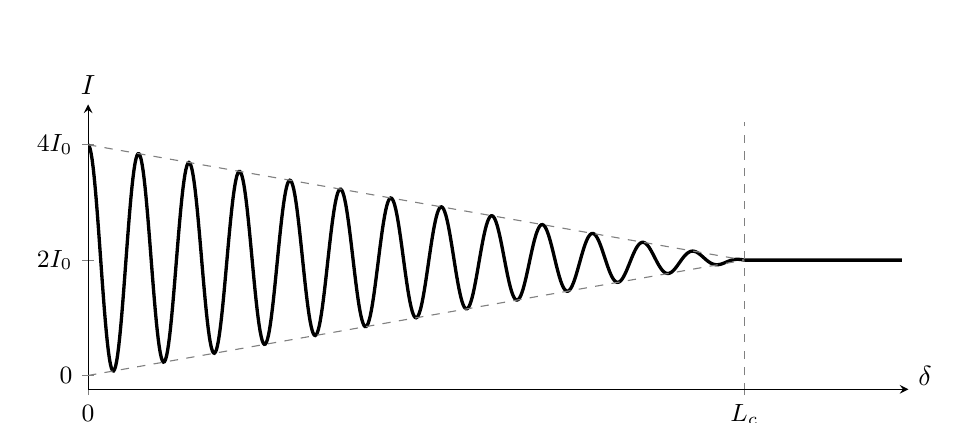
\begin{tikzpicture}
    \begin{axis}[
      width=12cm, height=5.2cm,
      axis lines=left,
      xmin=0, xmax=1.25, ymin=-0.12, ymax=2.35,
      xtick={0,1},
      xticklabels={$0$,$L_c$},
      ytick={0,1,2},
      yticklabels={$0$,$2I_0$,$4I_0$},
      xlabel={$\delta$},
      ylabel={$I$},
      every axis x label/.style={at={(current axis.right of origin)},anchor=west},
      every axis y label/.style={at={(current axis.above origin)},anchor=south},
      tick label style={font=\small},
      ]
      \addplot[very thick,domain=0:1.24,samples=800]
        {1 + max(0,1-x)*cos(deg(26*pi*x))};
      \addplot[gray,dashed,domain=0:1,samples=2]{2-x};
      \addplot[gray,dashed,domain=0:1,samples=2]{x};
      \draw[dashed,gray] (axis cs:1,0) -- (axis cs:1,2.2);
    \end{axis}
  \end{tikzpicture}

  \smallskip
  {\small\itshape Brouillage de franges: the contrast falls as $\delta$ approaches
  the longueur de cohérence $L_c$, beyond which the intensities merely add.}
\end{figure}

\subsubsection{Interférences entre deux ondes de couleurs différentes}

Lorsque la phase est aléatoire, le terme d'interférence est nul et les intensités
s'additionnent simplement. Or, le processus d'émission d'une source lumineuse
polychromatique fait qu'il n'y a \emph{pas de relation de phase entre deux
composantes de longueurs d'onde différentes}. En d'autres termes :

\begin{prop}
  Deux ondes de longueurs d'onde différentes n'interfèrent pas entre elles. Il
  suffit donc de sommer l'intensité des systèmes d'interférence créés par chaque
  longueur d'onde.
\end{prop}

Or, l'interfrange dépend de la longueur d'onde $\lambda$. The consequences in
white light are the following:

\begin{subpart}
  \item Pour $\delta = 0$, toutes les franges brillantes de chaque longueur d'onde
    sont superposées : \textbf{frange blanche} (\textit{white fringe}).
  \item Plus $\delta$ augmente, plus celles-ci se décalent spatialement. On voit
    donc apparaitre des \textbf{irisations} (\textit{iridescence}) appelées
    « \textbf{teintes de Newton} » (\textit{Newton tints}).
  \item Quand $\delta$ est trop grand, il y a brouillage des franges, on ne voit
    plus d'interférences. On parle de \textbf{blanc d'ordre supérieur}
    (\textit{white of higher order}).
\end{subpart}

\subsection{Irisation à la surface d'une nappe de pétrole}

Une nappe d'essence est une fine couche de quelques dixièmes de microns
d'épaisseur. Elle peut être assimilée à une fine lame d'indice $n$ à faces
parallèles. La lame est éclairée par une onde plane, le soleil par exemple.
Lorsque la lumière traverse ces dioptres, il se produit deux réflexions : une
première lors du passage de l'air à la couche d'indice, puis une deuxième
réflexion lors du passage de la couche d'indice à l'air. Les faisceaux émergents
sont parallèles, ils se croisent à l'infini. Là où ils se croisent, il peut se
former des interférences puisque ces deux faisceaux sont issus de la même source.

\begin{remark}
  The thickness is a few tenths of a micron, i.e.\ well under one $\mu$m: that is
  the figure that makes the physics work, since the thickness has to stay below the
  longueur de cohérence of white light.
\end{remark}

\subsubsection{Calcul de la différence de marche}

\begin{figure}[h!]
  \centering
  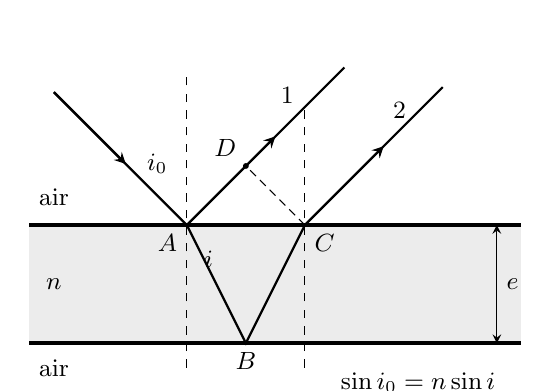
\begin{tikzpicture}[>=stealth,scale=1.25]
    % the plate
    \fill[gray!15] (-1.6,-1.2) rectangle (3.4,0);
    \draw[very thick] (-1.6,0) -- (3.4,0);
    \draw[very thick] (-1.6,-1.2) -- (3.4,-1.2);
    % normals
    \draw[dashed] (0,-1.45) -- (0,1.5);
    \draw[dashed] (1.2,-1.45) -- (1.2,1.2);
    % incident ray onto A
    \draw[thick] (-1.35,1.35) -- (0,0);
    \draw[->,thick] (-1.35,1.35) -- (-0.62,0.62);
    % reflected ray 1 at A
    \draw[thick] (0,0) -- (1.6,1.6);
    \draw[->,thick] (0,0) -- (0.9,0.9);
    \node at (1.02,1.32) {\small $1$};
    % inside: A -> B -> C
    \draw[thick] (0,0) -- (0.6,-1.2) -- (1.2,0);
    % emerging ray 2 at C
    \draw[thick] (1.2,0) -- (2.6,1.4);
    \draw[->,thick] (1.2,0) -- (2.0,0.8);
    \node at (2.16,1.16) {\small $2$};
    % D: foot of perpendicular from C onto ray 1
    \draw[densely dashed] (1.2,0) -- (0.6,0.6);
    \node[above left] at (0.6,0.6) {\small $D$};
    \fill (0.6,0.6) circle (0.03);
    % labels
    \node[below left] at (0,0) {\small $A$};
    \node[below] at (0.6,-1.2) {\small $B$};
    \node[below right] at (1.2,0) {\small $C$};
    \node at (-0.3,0.62) {\small $i_0$};
    \node at (0.22,-0.35) {\small $i$};
    \node at (-1.35,0.28) {\small air};
    \node at (-1.35,-0.6) {\small $n$};
    \node at (-1.35,-1.45) {\small air};
    \draw[<->] (3.15,0) -- (3.15,-1.2);
    \node[right] at (3.15,-0.6) {\small $e$};
    \node at (2.35,-1.6) {\small $\sin i_0 = n \sin i$};
  \end{tikzpicture}

  \smallskip
  {\small\itshape Lame d'indice $n$ à faces parallèles éclairée par une onde plane.
  Here $i$ is the angle \emph{inside} the plate. $D$ is the foot of the
  perpendicular dropped from $C$ onto ray $1$.}
\end{figure}

Un problème d'interférence commence par la résolution d'un problème géométrique.
La différence de chemin optique entre les faisceaux 1 et 2 est

\[ \Delta\ell = AB + BC - AD, \qquad
   \begin{cases}
     AB + BC = 2\,AB = 2n\dfrac{e}{\cos i}, \\[6pt]
     AD = AC \sin i_0 = 2 e \tan i \sin i_0,
   \end{cases} \]

with $i_0$ the angle of incidence in the air and $i$ the angle inside the plate,
$\sin i_0 = n \sin i$. Substituting,

\[ \Delta\ell = 2ne\left(\frac{1}{\cos i}
   - \tan i \underbrace{\frac{\sin i_0}{n}}_{\sin i}\right)
   = 2ne\,\frac{1 - \sin^{2} i}{\cos i}, \]

so that

\[ \boxed{\ \Delta\ell = \delta = 2ne\cos i \ }
   \qquad\Longrightarrow\qquad
   \boxed{\ \Delta\phi = \frac{2\pi}{\lambda}\,2ne\cos i \ } \]

\begin{remark}
  En réalité, la réflexion lame/air fait apparaître un déphasage supplémentaire
  de $\pi$ qui n'est pas pris en compte ici mais qui n'apporte rien au
  raisonnement et à la compréhension du phénomène. The formules de Fresnel above
  require it. It does swap the constructive and destructive conditions, so
  mention it if a problem asks for absolute orders.
\end{remark}

\subsubsection{Lame éclairée en lumière monochromatique}

Dans ce cas, $e$ est constant et c'est l'angle d'observation $i$ qui varie. À
l'infini, l'intensité varie suivant la formule de base des interférences à deux
ondes :

\[ I \simeq I_1 + I_2 + 2\sqrt{I_1 I_2}\,
   \cos\!\left(\frac{2\pi}{\lambda}\,2ne\cos i\right). \]

Donc, avec $m$ entier,

\[ \delta = 2ne\cos i = m\lambda
   \ \Longrightarrow\ i = \arccos\!\left(\frac{m\lambda}{2ne}\right)
   \qquad \text{(constructive)}, \]
\[ \delta = 2ne\cos i = (2m+1)\frac{\lambda}{2}
   \ \Longrightarrow\ i = \arccos\!\left(\frac{(2m+1)\lambda/2}{2ne}\right)
   \qquad \text{(destructive)}. \]

\begin{remark}
  Si on fait varier l'angle $i$, on parcourt donc les oscillations de $I$.
  Cependant, contrairement aux exemples précédemment rencontrés, la relation
  entre $\delta$ et $i$ n'est plus linéaire. Donc, sur un axe des angles
  d'incidence, les maxima de $I$ ne sont \emph{plus} également espacés.
\end{remark}

\subsubsection{Lame éclairée en lumière polychromatique : irisations}

L'angle pour lequel on obtient des interférences constructives dépend de
$\lambda$. Or, chaque figure d'interférence pour chaque longueur d'onde se somme
en intensité. Les couleurs se trouvent donc dispersées. These are the
\textit{irisations}.\\

L'observateur est fixe et observe des irisations. Lorsqu'il parcourt la surface
avec son œil, il change l'angle d'observation et donc la couleur sélectionnée. On
observe plusieurs ordres car $m$ peut valoir $1, 2, \dots$. La fonction
$\arccos(x)$ décroît lorsque $x$ augmente. Donc, \emph{quand $\lambda$
augmente, $i$ diminue}. Suivant la position de l'observateur qui regarde un
point donné de la surface, la couleur sélectionnée varie, ce qui est le cas
lorsqu'on se déplace devant une nappe irisée.

\begin{conclusion}[Why not in a bathtub]
  La réponse est directement liée à la longueur de cohérence de la lumière
  blanche, n'excédant pas quelques microns. Pour du pétrole, l'épaisseur est de
  quelques dixièmes de microns (well inside $L_c$) : les interférences sont donc
  visibles. Pour une baignoire ou une flaque d'eau, l'épaisseur est trop
  importante, bien supérieure à la longueur de cohérence d'une lumière blanche :
  les interférences sont invisibles.
\end{conclusion}

\begin{remark}
  On note sur une photo que les irisations prennent des formes irrégulières. En
  fait, cette figure d'interférence dépend de plusieurs paramètres : l'épaisseur
  de pétrole qui peut varier, les vagues qui font varier l'angle d'incidence.
  Enfin, cette démonstration est également valable pour une bulle de savon, mais
  les calculs de différence de marche sont à faire sur une sphère. C'est plus
  ardu.
\end{remark}

\subsection{Traitement anti-reflets}

Le principe des traitements anti-reflets consiste à recouvrir les dioptres de
couches transparentes minces dont l'épaisseur et l'indice sont soigneusement
déterminés, comme dans le cas précédent. Lorsque la lumière traverse un dioptre
ainsi traité, il se produit deux réflexions : une première lors du passage de
l'air à la couche anti-reflets (si la lentille est située dans l'air), puis une
deuxième réflexion lors du passage de la couche anti-reflets au verre. C'est le
fait de créer deux réflexions au lieu d'une qui va permettre d'obtenir l'effet
recherché. Si elles sont en opposition de phase, leurs effets se soustraient et
dans le cas idéal on obtient une interférence « destructive » supprimant la
réflexion. De ce fait, la lumière qui ne peut pas être réfléchie sur le dioptre
est transmise quasi intégralement par celui-ci.\\

Pour qu'une interférence destructive soit parfaite, deux conditions doivent être
réalisées. Il faut d'une part que les deux ondes aient exactement la même
amplitude et d'autre part qu'elles soient en exacte opposition de phase.

\begin{figure}[h!]
  \centering
  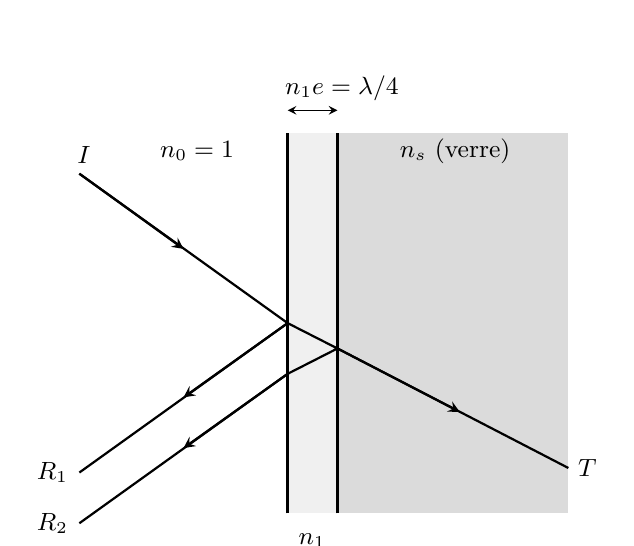
\begin{tikzpicture}[>=stealth,scale=1.15]
    \fill[gray!12] (0,-2.1) rectangle (0.55,2.1);
    \fill[gray!28] (0.55,-2.1) rectangle (3.1,2.1);
    \draw[very thick] (0,-2.1) -- (0,2.1);
    \draw[very thick] (0.55,-2.1) -- (0.55,2.1);
    % thickness marker
    \draw[<->] (0,2.35) -- (0.55,2.35);
    \node[above] at (0.6,2.35) {\small $n_1 e = \lambda/4$};
    % indices
    \node at (-1.0,1.9) {\small $n_0 = 1$};
    \node at (0.27,-2.4) {\small $n_1$};
    \node at (1.85,1.9) {\small $n_s$ (verre)};
    % incident
    \draw[thick] (-2.3,1.65) -- (0,0);
    \draw[->,thick] (-2.3,1.65) -- (-1.15,0.82);
    \node[above] at (-2.25,1.65) {\small $I$};
    % R1
    \draw[thick] (0,0) -- (-2.3,-1.65);
    \draw[->,thick] (0,0) -- (-1.15,-0.82);
    \node[left] at (-2.32,-1.65) {\small $R_1$};
    % inside
    \draw[thick] (0,0) -- (0.55,-0.28) -- (0,-0.56);
    % R2
    \draw[thick] (0,-0.56) -- (-2.3,-2.21);
    \draw[->,thick] (0,-0.56) -- (-1.15,-1.38);
    \node[left] at (-2.32,-2.21) {\small $R_2$};
    % T
    \draw[thick] (0.55,-0.28) -- (3.1,-1.6);
    \draw[->,thick] (0.55,-0.28) -- (1.9,-0.98);
    \node[right] at (3.1,-1.6) {\small $T$};
  \end{tikzpicture}

  \smallskip
  {\small\itshape Double réflexion obtenue avec une lame quart d'onde. $R_1$ and
  $R_2$ are made equal in amplitude and
  opposite in phase, so the reflection cancels and everything goes into $T$.}
\end{figure}

\paragraph{Même amplitude.} La réflexion sur un dioptre dépend directement de la
différence des indices de réfraction des deux milieux ; dans le cas d'une
incidence normale, on admet que le coefficient de réflexion en amplitude sur un
dioptre séparant 2 milieux d'indices $n_1$ et $n_2$ vaut

\[ r = \frac{n_2 - n_1}{n_2 + n_1}, \]

soit, pour une couche anti-reflet composée de 2 dioptres air/anti-reflet et
anti-reflet/verre,

\[ r_{\text{air}/\text{anti-reflet}}
     = \frac{n_{\text{anti-reflet}} - 1}{n_{\text{anti-reflet}} + 1},
   \qquad
   r_{\text{anti-reflet}/\text{verre}}
     = \frac{n_{\text{verre}} - n_{\text{anti-reflet}}}
            {n_{\text{verre}} + n_{\text{anti-reflet}}} . \]

Setting $r_{\text{air}/\text{anti-reflet}} = r_{\text{anti-reflet}/\text{verre}}$,
on montre facilement que la couche anti-reflets doit posséder un indice

\[ \boxed{\ n_{\text{anti-reflet}} = \sqrt{n_{\text{verre}}}\ } \]

\begin{example}
  Avec un verre d'indice $1{,}69$, il faut une couche d'indice $1{,}3$ pour
  réaliser l'égalité des amplitudes.
\end{example}

\paragraph{Opposition de phase.} La lumière réfléchie sur le second dioptre doit
être décalée d'une demi-longueur d'onde par rapport à celle que renvoie le
premier. La couche est traversée deux fois par la seconde onde réfléchie. With
$\delta = 2ne$, then,

\[ \Delta\varphi = \frac{2\pi \cdot 2ne}{\lambda} = m\pi
   \qquad\Longrightarrow\qquad
   \boxed{\ ne = m\,\frac{\lambda}{4}\ } \]

with $m$ odd for the destructive case: the first solution is the
\textbf{lame quart d'onde} (\textit{quarter-wave layer}), of optical thickness
$ne = \lambda/4$, i.e.\ a quarter of a longueur
d'onde \emph{measured inside the coating}.

\begin{remark}[Limits of a single layer]
  En incidence normale, la correction fournie par le traitement n'est en principe
  valable que pour une seule longueur d'onde. Si l'incidence de la lumière n'est
  pas normale au dioptre, le chemin optique se trouve allongé et la correction
  fonctionne encore mais pour une longueur d'onde un peu plus grande, donc pour un
  rayonnement décalé vers le rouge. En pratique, l'amélioration concerne presque
  tout le spectre visible, mais il n'est pas possible avec une seule épaisseur de
  traitement d'obtenir une interférence parfaitement destructive pour toutes les
  longueurs d'onde et pour tous les angles d'incidence. Il faut donc savoir en
  fonction de quelle longueur d'onde, c'est-à-dire en fonction de quelle couleur,
  cette épaisseur sera choisie. Les lentilles qui portent un traitement
  monocouche ont donc forcément un aspect coloré. La plupart du temps elles
  semblent bleutées, ce qui signifie que l'on a privilégié l'absence de réflexion
  de la couleur complémentaire, c'est-à-dire le jaune, qui est la couleur la plus
  éblouissante, qui du coup sera davantage transmis. Les traitements multicouches
  évitent la réflexion de deux ou plusieurs longueurs d'onde différentes ; les
  lentilles apparaissent alors beaucoup moins teintées que dans le cas d'un
  traitement monocouche. Cependant, le traitement mono-couche est bon marché, donc
  accessible au grand public sur les verres de lunettes de vue.
\end{remark}

\begin{conclusion}[What the course expects from this chapter]
  Comprendre la notion de chemin optique ; savoir appliquer les lois de la
  réflexion et de la réfraction ; savoir calculer l'angle limite de réflexion
  totale ; savoir calculer et représenter la figure d'interférence entre deux
  ondes planes cohérentes ; savoir calculer une longueur de cohérence ; savoir
  déterminer les conditions d'obtention d'interférences ; et savoir expliquer et
  calculer les positions des irisations sur une nappe de pétrole.
\end{conclusion}

\section{Ondes électromagnétiques et analyse spectrale}

L'optique géométrique décrit le chemin suivi par un fin faisceau de lumière sans
se préoccuper de la nature physique profonde de la lumière. Or, on sait que de
l'énergie est véhiculée par un faisceau lumineux puisque les rayons lumineux nous
chauffent, qu'un faisceau laser peut mettre le feu à une feuille de papier noir
ou encore qu'un faisceau lumineux peut provoquer une réaction chimique et
impressionner un film photographique ou les cellules de notre rétine. Objectifs
pédagogiques : savoir exprimer une onde plane et une onde sphérique ; comprendre
la notion de transformée de Fourier --- the tool the rest of the module runs on.

\subsection{Expression d'une vibration lumineuse monochromatique}

\subsubsection{Généralités sur les équations de Maxwell}

C'est dès le XVII\textsuperscript{e} siècle, à partir d'observations
expérimentales des phénomènes d'interférences et de diffraction, que l'on a
compris que la lumière était un phénomène ondulatoire (Huygens 1629--1695, Young
1773--1829, Malus 1775--1812). Mais il a fallu attendre Maxwell (1831--1879) pour
qu'on comprenne que la grandeur physique qui se propageait en vibrant était un
\textbf{champ électrique} (\textit{electric field}) $\v{E}$, accompagné d'un
\textbf{champ magnétique} (\textit{magnetic field}) $\v{B}$, et que cette onde,
dite onde électromagnétique, pouvait se propager dans le vide avec une vitesse
appelée célérité :

\[
  c=\frac{1}{\sqrt{\varepsilon_0\mu_0}}\approx 3\cdot 10^{8}\ \mathrm{m/s},
  \qquad
  \varepsilon_0=8.854\cdot 10^{-12}\ \mathrm{A\,s\,V^{-1}m^{-1}},
  \qquad
  \mu_0=4\pi\cdot 10^{-7}\ \mathrm{kg\,m\,A^{-2}s^{-2}} .
\]

Dans un milieu matériel, la permittivité et la perméabilité s'écrivent
$\varepsilon$ et $\mu$.

\begin{definition}[Onde (\textit{wave})]
  Une onde est un phénomène physique de \emph{transport d'énergie sans
  transport de matière}. C'est le même cas pour une vague sur l'océan ou une
  onde sismique lors d'un tremblement de terre.
\end{definition}

Établir en détail les \textbf{équations de Maxwell} (\textit{Maxwell's
equations}) dépasse le cadre de ce cours et sera discuté dans le module COM103
« Propagation ». Nous en admettrons les résultats utiles pour la suite.

\begin{prop}[Conséquences des équations de Maxwell]
  Les équations de Maxwell montrent, pour les champs de l'onde
  électromagnétique, que :
  \begin{itemize}
    \item Un champ électrique et un champ magnétique variables dans le temps ne
      restent pas localisés dans une région de l'espace : la variation
      temporelle du champ électromagnétique est forcément associée à une
      propagation spatiale de ce dernier.
    \item Les ondes électromagnétiques (EM) sont \textbf{transverses},
      c'est-à-dire qu'en tout point, les grandeurs vibrantes $\v{E}$ et
      $\v{B}$ sont dans un plan perpendiculaire à la direction de propagation
      $\v{k}$, le \textbf{vecteur d'onde} (\textit{wave vector}).
    \item Ces champs sont \textbf{couplés} : on peut déduire $\v{B}$ de la
      connaissance de $\v{E}$ sur tout l'espace (et réciproquement) via les
      équations de Maxwell. On ne s'intéressera donc qu'au champ électrique
      $\v{E}$.
    \item Dans le vide infini, les \textbf{ondes planes} (\textit{plane wave})
      sont des solutions des équations de Maxwell. La direction $\v{k}$ est
      fixée ainsi que les directions de $\v{E}$ et $\v{B}$. Ces trois vecteurs
      forment un trièdre trirectangle --- a right-handed one. À tout instant,
      on montre que $|\v{E}|=c\,|\v{B}|$ (où $|\v{E}|$ et $|\v{B}|$
      représentent les amplitudes crêtes des champs qui oscillent).
  \end{itemize}
\end{prop}

\begin{remark}
  Tout ceci n'est pas exact dans un milieu inhomogène ou anisotrope !
\end{remark}

\begin{figure}[h!]
  \centering
  \begin{tikzpicture}[>=stealth,scale=1.0]
    \draw[->,thick] (0,-1.6) -- (0,2.0) node[above] {$x$};
    \draw[->,thick] (-0.5,0) -- (6.2,0) node[right] {$z$};
    \draw[->,thick] (0.55,0.42) -- (-1.45,-1.1) node[below left] {$y$};
    \draw[red,thick,domain=0:5.2,samples=160,smooth,variable=\z]
      plot ({\z},{1.3*sin(\z*100)});
    \draw[blue,thick,domain=0:5.2,samples=160,smooth,variable=\z]
      plot ({\z-0.45*sin(\z*100)},{-0.35*sin(\z*100)});
    \draw[->,very thick,red] (0.9,0) -- (0.9,1.3) node[above] {$\v{E}$};
    \draw[->,very thick,blue] (0.9,0) -- (0.45,-0.35) node[below left] {$\v{B}$};
    \draw[->,very thick] (5.3,0) -- (6.0,0) node[above] {$\v{k}$};
  \end{tikzpicture}
  \caption*{\small The trirectangular trihedron $(\v{E},\v{B},\v{k})$ of a
  transverse onde plane polarised along $Ox$ and propagating along $Oz$.}
\end{figure}

Dans le cas d'un milieu diélectrique homogène, isotrope et permanent --- un
\textbf{diélectrique} (\textit{dielectric}) est un matériau qui ne contient pas
de charges électriques susceptibles de se déplacer de façon macroscopique, c'est
donc un milieu qui ne conduit pas le courant, comme l'air ou le verre par
exemple --- les équations de Maxwell permettent d'établir
l'\textbf{équation de Helmholtz} (\textit{Helmholtz equation}), une équation de
propagation pour $\v{E}$ (indépendamment du champ magnétique) :

\[
  \nabla^2\v{E}-\varepsilon\mu\,\frac{\del^2\v{E}}{\del t^2}=0,
  \qquad
  \nabla^2=\Delta=\frac{\del^2}{\del x^2}+\frac{\del^2}{\del y^2}+\frac{\del^2}{\del z^2}.
\]

Ses solutions permettent de connaître l'évolution spatio-temporelle
$\v{E}(x,y,z,t)$.

\subsubsection{Intuitivement}

Chacun a déjà jeté un caillou dans l'eau ou agité une cordelette avec la main.
Intuitivement, on aurait envie d'exprimer cette oscillation périodique
temporelle de l'eau à l'endroit où le caillou est tombé, en $z=0$, par une
expression sinusoïdale dépendant du temps :

\[
  E(t)\big|_{z=0}=E_0\cos\!\left(\frac{2\pi t}{T_0}\right)=E_0\cos 2\pi\nu_0 t=E_0\cos\omega_0 t,
\]

où $E_0$ est l'amplitude de l'oscillation, $T_0$ est la période d'oscillation,
$\nu_0$ est la fréquence et $\omega_0$ la pulsation. Par contre, l'observateur
retiendra plutôt de ce jet de caillou que des anneaux s'éloignent de l'endroit où
est tombé ce dernier. Il retiendra de la cordelette agitée qu'une onde se propage
le long de cette dernière. Il manque donc une information : simultanément à
l'oscillation temporelle, une onde se propage spatialement ! C'est d'ailleurs ce
que nous dit l'équation de propagation. Si l'onde se propage à la vitesse $v$, à
une distance $z$ de la main, la vibration sera à l'instant $t$ ce qu'elle était
à l'origine à l'instant $t-z/v$. On peut donc réécrire l'équation en remplaçant
$t$ par $t-z/v$, puis en séparant ce qui dépend du temps de ce qui dépend de
l'espace :

\begin{align*}
  E(t,z)&=E_0\cos\!\left(\frac{2\pi}{T_0}\left(t-\frac{z}{v}\right)\right)
  =E_0\cos\!\left(2\pi\Big(\underbrace{\tfrac{t}{T_0}}_{\text{temporal period}}
    -\underbrace{\tfrac{z}{\lambda}}_{\text{spatial period}}\Big)\right)\\
  &=E_0\cos\big(\underbrace{\omega_0t}_{\text{temporal phase}}
    -\underbrace{\varphi}_{\text{spatial phase}}\big),
\end{align*}

avec $\lambda=vT_0$ et $\varphi=2\pi z/\lambda$. À un endroit donné, à chaque
durée $T_0$, le cosinus accumulera $2\pi$ de phase ; à un instant donné, à chaque
distance $\lambda$, le cosinus accumulera également $2\pi$ de phase.
$\omega_0t-\varphi$ est appelée simplement \textbf{phase}. Sans le savoir, nous
avons résolu de manière intuitive l'équation de propagation pour une onde se
propageant suivant $z$ ! On va voir que la solution trouvée est appelée onde
plane.

\subsubsection{Définition : pulsation, fréquence, longueur d'onde}

\begin{definition}[Pulsation, longueur d'onde, vecteur d'onde]
  La \textbf{pulsation} $\omega$ est reliée à la fréquence $\nu$ et à la
  période temporelle $T$ par l'expression $\omega=2\pi\nu=2\pi/T$. La
  \textbf{longueur d'onde} (\textit{wavelength}) $\lambda$ représente la
  période d'oscillation spatiale du champ électrique. Elle est reliée à la
  phase par l'expression $\varphi=2\pi z/\lambda$. Le vecteur d'onde $\v{k}$
  est quant à lui le vecteur qui porte la direction de propagation, de module
  $|\v{k}|=2\pi/\lambda$.
\end{definition}

Puisque la vitesse de propagation dépend du milieu traversé, il en est de même
pour la longueur d'onde :

\[
  \lambda=\frac{\lambda_0}{n},
\]

avec $\lambda_0$ la longueur d'onde dans le vide et $n$ l'indice du milieu.
Enfin, pulsation et fréquence sont reliées dans le vide à la longueur d'onde
par :

\[
  \omega=2\pi\nu=\frac{2\pi c}{\lambda}
  \quad\text{so}\quad \lambda=\frac{c}{\nu},
  \qquad\text{and in a medium of index }n:\quad
  |\v{k}|=\frac{2\pi}{\lambda}=\frac{\omega n}{c}
  \quad\text{so}\quad \lambda=\frac{c}{n\nu}.
\]

\begin{remark}
  La longueur d'onde varie avec le milieu traversé, pas la \emph{fréquence} !
  Attention, il ne faut donc pas confondre d'un côté fréquence (ou pulsation)
  et de l'autre longueur d'onde bien que ces variables soient reliées dans le
  vide : l'une informe sur l'oscillation dans le temps alors que l'autre
  l'oscillation dans l'espace. Elles ne représentent pas la même grandeur
  physique.
\end{remark}

\subsubsection{Notion de polarisation de la lumière et approche scalaire}

Imaginons une corde tendue horizontalement. Si nous agitons une extrémité de
haut en bas dans un plan vertical, l'ébranlement se propage tout en restant dans
le plan vertical. Nous avons alors fabriqué une onde polarisée rectilignement. Ce
plan vertical est appelé \textbf{plan de polarisation} (\textit{plane of
polarisation}). Il en va de même pour le champ électrique.

\begin{definition}[État de polarisation (\textit{polarisation state})]
  L'état de polarisation d'une onde lumineuse est défini par la direction du
  champ électrique (ou magnétique) au cours de sa propagation :
  \begin{itemize}
    \item \textbf{Polarisation rectiligne} (\textit{rectilinear polarisation}) :
      les champs $\v{E}$ et $\v{B}$ gardent une direction déterminée au cours
      de la propagation. Le plan défini par $\v{E}$ et $\v{k}$ est alors appelé
      plan de polarisation.
    \item \textbf{Polarisation circulaire ou elliptique} (\textit{circular or
      elliptical polarisation}) : le champ électrique peut être considéré comme
      la somme de deux champs perpendiculaires et déphasés qui se propagent
      suivant la même direction. Le résultat est que l'extrémité de $\v{E}$, au
      contraire de la polarisation rectiligne, ne reste pas dans le plan de
      polarisation. Si on regarde l'onde venant de face, l'extrémité du champ
      électrique décrit un cercle ou une ellipse.
    \item \textbf{Lumière non polarisée} (\textit{unpolarised light}) : une
      onde est non polarisée si $\v{E}$ a une direction qui varie aléatoirement
      dans le plan d'onde (lumière du soleil par exemple).
  \end{itemize}
\end{definition}

\begin{notation}[The scalar simplification]
  On dira que l'onde est polarisée rectilignement suivant $Ox$ --- a choice
  kept throughout the module. Ainsi, nous réduisons notre problème vectoriel à
  un système \emph{scalaire} : le cadre de ce cours se situe en
  \textbf{optique ondulatoire scalaire} (\textit{scalar wave optics}).
\end{notation}

\subsubsection{La solution formelle : l'onde plane}

On pourrait valider notre étude intuitive en résolvant formellement l'équation
de propagation. En choisissant $\v{k}$ parallèle à l'axe $Oz$, la résolution
formelle montre que le champ électrique peut s'écrire en notation réelle comme :

\[
  \left\{
  \begin{aligned}
    E^{(r)}_x&=E_0\cos\!\left(\omega\left(t-\frac{z}{v_\phi}\right)-\phi_0\right)
             =E_0\cos\!\left(\omega t-2\pi\frac{z}{\lambda}-\phi_0\right)\\
    E^{(r)}_y&=0 \quad\to\quad \text{wave polarised along } Ox\\
    E^{(r)}_z&=0 \quad\to\quad \text{transverse wave}
  \end{aligned}
  \right.
\]

où $v_\phi$ est la vitesse de propagation de l'onde, et $\phi_0$ la phase à
l'origine de l'espace et du temps (arbitraire).

\begin{remark}[Limits of this solution]
  Cette onde est transverse car la composante du champ suivant $z$ est nulle :
  $\v{E}$ oscille donc dans le plan $xOy$ perpendiculaire à la direction de
  propagation. Cette solution n'est vraie que pour un espace infini, uniforme,
  isotrope et permanent. Sinon, les calculs sont beaucoup plus compliqués. Nous
  avons choisi de présenter une solution dont la polarisation est rectiligne,
  suivant $x$ --- a choice, not a necessity.
\end{remark}

\subsubsection{Représentation d'une onde plane}

La phase spatiale étant $\varphi=2\pi z/\lambda$, à $z$ donné, la phase
accumulée par le champ électrique est la même partout dans le plan $xOy$,
quelles que soient $x$ et $y$ : la \textbf{surface équiphase} (\textit{equiphase
surface}) est un plan. D'où la dénomination d'onde plane, and one speaks of the
\textbf{plan d'onde} (\textit{wave plane}). On représente généralement les plans
pour lesquels $\varphi(\v{r})=2q\pi$ avec $q$ entier. Spatialement, l'onde plane
se déplace suivant $z$, parcourant la distance $z_2-z_1=\frac{c}{n}(t_2-t_1)$ ;
temporellement, à un endroit donné, l'onde oscille dans le temps avec une
période temporelle $1/\nu$.

\begin{remark}[Superposition]
  Les ondes planes ne sont pas les seules solutions des équations de Maxwell,
  bien au contraire. Par contre, ces solutions sont primordiales car on peut
  montrer que toute autre solution peut s'écrire comme combinaison linéaire
  d'ondes planes (dont les pulsations de chaque composante ainsi que les
  directions et amplitudes des champs électriques ne sont pas forcément toutes
  les mêmes). C'est le principe de superposition. Par ailleurs, pour une onde
  plane, ce plan est théoriquement infini suivant $x$ et $y$. Il revêt donc
  clairement un aspect théorique : une des ondes les plus planes qui soient que
  l'on peut rencontrer sur terre est la lumière du soleil (qui s'étend quand
  même sur $0.5^\circ$) voire mieux, celle des étoiles lointaines.
\end{remark}

\subsubsection{Notation complexe d'une onde plane}

Il est commode de représenter la vibration réelle par son expression complexe,
dont elle est la partie réelle. Les calculs sont alors grandement simplifiés !

\begin{definition}[Signal analytique (\textit{analytic signal})]
  En notation complexe, la fonction d'onde monochromatique plane est appelée
  signal analytique et a pour expression :
  \begin{align*}
    E(\v{r},t)&=E_0\exp\Big(i\big(\underbrace{\omega t}_{\text{temporal phase}}
      -\underbrace{\v{k}\cdot\v{r}}_{\text{spatial phase}}
      -\underbrace{\phi_0}_{\text{phase at origin}}\big)\Big)
    =E_0\exp\big(i(\omega t-(k_xx+k_yy+k_zz)-\phi_0)\big)\\
    &=\underbrace{E(\v{r})}_{\text{complex amplitude}}\cdot
      \underbrace{\exp(i\omega t)}_{\text{temporal oscillation}} .
  \end{align*}
\end{definition}

L'argument de l'exponentielle, $\omega t-\v{k}\cdot\v{r}-\phi_0$, est appelé
phase de l'onde ; $\omega t$ est la phase temporelle de l'onde ; la quantité
complexe $e^{i\omega t}=e^{2i\pi\nu t}$ rend compte de l'oscillation temporelle
de l'onde ; la quantité $E(\v{r})=E_0\exp(-i(\v{k}\cdot\v{r}+\phi_0))$ désigne
l'\textbf{amplitude complexe} (\textit{complex amplitude}) de l'onde, dont
l'argument $\v{k}\cdot\v{r}+\phi_0$ est la phase spatiale de l'onde (souvent
appelée simplement sa phase). La phase à l'origine $\phi_0$ est généralement
inconnue et donc choisie de manière arbitraire. Enfin, $\v{k}\cdot\v{r}$
représente le produit scalaire entre le vecteur d'onde et le vecteur position.

\begin{remark}
  $E_0$ s'exprime en V/m. Son intégration de $-\infty$ à $+\infty$ est infinie,
  ceci montre qu'une onde plane n'est pas physiquement acceptable. Par contre,
  les solutions réelles, combinaisons d'ondes planes, le sont !
\end{remark}

Nous pouvons ainsi manipuler les exponentielles pour effectuer n'importe quel
calcul puis retourner à la forme en cosinus de l'onde en prenant la partie réelle
du résultat et ainsi faire une interprétation physique.

\begin{example}[Writing two ondes planes]
  \begin{subpart}
    \item Une onde plane incidente parallèle à l'axe de propagation $Oz$ et dont
      la norme du vecteur d'onde est $|\v{k}|=k_0$ :
      \[
        E(\v{r},t)=E(z,t)=E_0\,e^{i(\omega t-k_0z-\phi_0)},
        \qquad\text{and at } z=t=\phi_0=0,\quad E=E_0 .
      \]
    \item Une onde dont la direction du vecteur $\v{k}$ fait un angle $\theta$
      avec l'axe $Oz$ dans le plan $(xOz)$ : on peut écrire
      $\v{k}\cdot\v{r}=k_xx+k_yy+k_zz=k_0x\sin\theta+k_0z\cos\theta$, d'où
      \[
        E(\v{r},t)=E(x,y)E(z,t)=E_0
        \underbrace{e^{i(\omega t-k_0z\cos\theta)}}_{\text{plane wave} \parallel Oz}
        \underbrace{e^{-i(k_0x\sin\theta)}}_{\text{dephasing }\phi(x,y)} .
      \]
  \end{subpart}
\end{example}

\subsubsection{Énergie d'une onde lumineuse}

\begin{definition}[Intensité lumineuse (\textit{light intensity})]
  On appelle intensité lumineuse le flux d'énergie moyen associé à l'onde
  électromagnétique, c'est-à-dire l'énergie moyenne traversant par unité de
  temps une surface unité, perpendiculaire à la direction de propagation, soit :
  \[
    I=\varepsilon_0c\left\langle E^2\right\rangle
     =\varepsilon_0c\,\frac{1}{T_D}\int_0^{T_D}\big|\v{E}\big|^2\,dt ,
  \]
  où $T_D$ est le temps d'intégration du détecteur relié à la bande passante du
  détecteur par $BP=1/T_D$. Pour les plus physiciens d'entre vous, on parle de
  flux du vecteur de Poynting à travers une surface fermée.
\end{definition}

La bande passante des meilleurs détecteurs est de l'ordre de quelques 100 GHz,
whereas an onde optique oscillates far faster. Le détecteur ne peut donc voir
l'oscillation du champ, il ne peut en mesurer qu'une moyenne ! La valeur moyenne
d'une onde plane sur une période de détection $T_D$ grande devant la période
d'oscillation $T$ du champ étant $T_D/2$, on obtient :

\[
  I=\frac{1}{2}\varepsilon_0cE_0^2
  \qquad\text{and in practice we use}\qquad
  \boxed{\,I\propto EE^{*}=|E_0|^{2}\,}
\]

Ainsi, la puissance moyenne transportée par une onde monochromatique est
proportionnelle au carré de l'amplitude réelle, c'est-à-dire au carré du module
de l'amplitude complexe. C'est l'expression que l'on utilisera pour calculer
l'intensité lumineuse d'une onde. Notez que l'intensité d'une onde
monochromatique ne varie pas dans le temps !

\begin{remark}
  An onde optique oscillates far faster than any detector responds: the
  classification of radiations below puts the visible between
  $3.75\cdot 10^{14}$ and $7.5\cdot 10^{14}$ Hz, i.e. hundreds of THz. The
  detector bande passante is therefore orders of magnitude below the optical
  frequency, so only $\langle E^2\rangle$ is observable.
\end{remark}

\subsubsection{Remarque sur les variables $t$ et $z$ et la constante $\phi_0$}

Une onde plane s'écrit en toute généralité :

\[
  E(\v{r},t)=E_0\,E(x,y)\,E(z,t)=E_0\,e^{-(ik_xx+ik_yy)}\,e^{i\omega t}e^{-ik_zz}e^{-i\phi_0}.
\]

Dans toutes les expériences que nous mènerons : $\phi_0$ est inconnue ; de plus,
pour des raisons de cohérence, toutes les ondes proviendront de la même source,
on choisit $\phi_0=0$ ; le sens de propagation est suivant $z$, on peut placer
notre expérience en $z=0$ sans perte de généralité ; nos expériences sont
effectuées à l'instant $t_0$, on peut effectuer notre expérience en $t=0$ sans
perte de généralité. Ainsi on pourra choisir sans perte de généralité :
$e^{i\omega t}e^{-ik_zz}e^{-i\phi_0}=1$. On peut également garder ces termes
explicitement : lorsqu'on calculera l'intensité de l'onde, leur module sera de
toutes les manières égal à $1$ ! On peut donc écrire l'expression d'une onde
plane dans le cas général :

\[
  E(\v{r},t)\Big|_{\substack{z=0\\ t=0\\ \phi_0=0}}=E_0\,E(x,y)=E_0\,e^{-(ik_xx+ik_yy)} .
\]

\subsubsection{Vitesse de phase}

La vitesse de propagation de l'onde est la vitesse avec laquelle les plans
d'égale phase se déplacent, d'où le nom de vitesse de phase :

\[
  v_\phi=\frac{\omega}{k}=\frac{c}{n}.
\]

\subsubsection{Lien entre onde plane et optique géométrique}

Dans le cas d'une onde plane, le vecteur d'onde est unique. Il est par ailleurs,
par définition, perpendiculaire à la surface d'onde, c'est-à-dire parallèle à la
direction de propagation. Un tel faisceau peut être représenté, en optique
géométrique, par une série de rayons parallèles, que l'on appelle également
\textbf{faisceau collimaté} (\textit{collimated beam}).

\begin{remark}
  Le principe de Fermat stipule que la trajectoire suivie par un rayon entre un
  point $A$ et un point $B$ est celle qui minimise le temps de trajet (donc le
  chemin optique). Ce principe permet de déduire l'équation différentielle de la
  trajectoire d'un rayon lumineux, dite équation « eikonale ». De là, on peut
  démontrer que les rayons en optique géométrique sont $\perp$ aux surfaces
  équiphases en optique ondulatoire, donc $\parallel$ à $\v{k}$. Le rayon est
  donc équivalent à $\langle\v{\pi}\rangle$ où $\v{\pi}$ est le vecteur de
  Poynting.
\end{remark}

\paragraph{Onde plane parallèle à $Oz$.} On peut écrire l'expression d'une
onde plane parallèle à $Oz$, en $z=0$ :

\[
  E_{\text{plane wave}}(x,y,z)\Big|_{\substack{\perp\ \text{incidence}\\ z=0}}
  \propto e^{-i\v{k}\cdot\v{r}}=e^{-i(k_xx+k_yy+k_zz)}
  \propto \underbrace{\mathbf{1}(x,y)}_{=1\ \forall x,y} .
\]

\paragraph{Onde plane en incidence oblique.} On peut écrire l'expression d'une
onde plane en incidence oblique $\theta$ :

\begin{align*}
  E_{\text{plane wave}}(x,y,z)\Big|_{\substack{\text{incidence }\theta\\ z=0}}
  &=e^{-i(k_xx+k_yy+k_zz)}=e^{-i(k_0x\sin\theta+k_0z\cos\theta)}
  \propto e^{-ik_0x\sin\theta}\\
  &\propto e^{-ik_0x\theta}\quad\text{if }\theta\text{ is small (paraxial optics)}.
\end{align*}

\begin{conclusion}
  Une onde plane en incidence oblique apparaît donc mathématiquement comme une
  onde plane $\parallel Oz$ \emph{déphasée} dans les directions $x$ ou $y$. An
  angle is a phase delay $\phi(x)$ --- this identification is the hinge on which
  the whole Fourier-optics chapter turns.
\end{conclusion}

\begin{figure}[h!]
  \centering
  \begin{tikzpicture}[>=stealth,scale=0.9]
    \foreach \i in {0,...,5}{\draw[red,thick] (\i*0.55,-1.1) -- (\i*0.55,1.1);}
    \draw[<->] (0,-1.35) -- (0.55,-1.35) node[midway,below,font=\small] {$\lambda$};
    \draw[->,very thick] (1.1,0) -- (2.2,0) node[above,font=\small] {$\v{k}$};
    \node[font=\small] at (1.4,1.5) {incidence $\perp$};
    \begin{scope}[xshift=5.4cm]
      \begin{scope}[rotate around={-30:(1.4,0)}]
        \foreach \i in {0,...,5}{\draw[red,thick] (\i*0.55,-1.1) -- (\i*0.55,1.1);}
        \draw[->,very thick] (1.1,0) -- (2.5,0);
      \end{scope}
      \draw[dashed] (1.4,0) -- (3.5,0) node[right,font=\small] {$z$};
      \draw (2.02,0) arc (0:-30:0.62);
      \node[font=\small] at (2.24,-0.21) {$\theta$};
      \node[font=\small] at (2.85,-0.78) {$\v{k}$};
      \node[font=\small] at (1.4,1.75) {incidence $\theta$};
    \end{scope}
  \end{tikzpicture}
  \caption*{\small Equiphase planes at a fixed instant. Left: an onde
  $\parallel Oz$; right: oblique incidence, equivalent in optique géométrique to
  a tilted bundle of parallel rays.}
\end{figure}

\subsubsection{Classification des radiations}

Une onde électromagnétique reste une onde électromagnétique, quelle que soit sa
fréquence, et se propage à la vitesse de la lumière dans le vide, $c$. Seules des
raisons de commodité technique ou d'usage font établir des divisions dans cet
ensemble : aucun milieu n'est transparent pour toutes ces radiations, et il
n'existe pas de source unique permettant d'obtenir l'intégralité du spectre
électromagnétique avec une intensité suffisante, ni de détecteur capable de
détecter toutes les fréquences simultanément du Hz à plus de $10^{20}$ Hz.\\

Le domaine du visible ne représente qu'une toute petite partie des longueurs
d'onde possibles des ondes électromagnétiques, de $0.4$ à $0.8\ \mu$m ($400$ nm
de bande passante !). Ces bornes sont en fait les limites de sensibilité de
l'œil. In frequency the visible runs from $3.75\cdot 10^{14}$ Hz ($0.8\ \mu$m)
to $7.5\cdot 10^{14}$ Hz ($0.4\ \mu$m); the last entry of the table below,
$745$ nm $\leftrightarrow$ $405$ THz, stops short of that edge. Pour
l'opticien, le domaine de l'optique est un peu plus large puisqu'il englobe le
domaine de l'ultraviolet et de l'infrarouge. On parle de lumière
\textbf{monochromatique} (\textit{monochromatic}) lorsque toutes les ondes
constituant le rayonnement sont toutes de la même fréquence.

\begin{center}
  \small
  \begin{tabular}{lcccccccc}
    \toprule
    $\lambda$ (nm) & 400 & 435 & 490 & 520 & 565 & 590 & 625 & 745 \\
    $\nu$ (THz)    & 750 & 690 & 612 & 577 & 530 & 508 & 480 & 405 \\
    \bottomrule
  \end{tabular}
\end{center}

\begin{remark}[Lien entre fréquence, longueur d'onde et couleur]
  Fréquence et longueur d'onde dans le vide sont liées. La première correspond à
  une oscillation temporelle alors que la seconde à une oscillation spatiale.
  Cependant, la fréquence d'un rayonnement est indépendante du milieu qu'il
  traverse. Par contre, la longueur d'onde varie avec l'indice du milieu
  traversé. En réalité, les détecteurs sont sensibles à la moyenne de
  l'oscillation \emph{temporelle} du champ et non à l'oscillation spatiale. Ils
  sont donc sensibles à la fréquence et non à la longueur d'onde. À l'œil nu,
  par exemple, du bleu reste bleu quel que soit le milieu, donc quel que soit
  l'indice de réfraction ! En fait, lorsque l'on fait l'amalgame entre fréquence
  et longueur d'onde, on sous-entend que l'on exprime cette dernière dans le
  vide ! La notion de couleur représente elle la perception subjective qu'a
  l'œil d'une ou plusieurs fréquences d'ondes lumineuses, avec une (ou des)
  amplitude(s) donnée(s). On assimile également souvent en optique couleur à
  longueur d'onde monochromatique de manière abusive. On utilisera parfois dans
  la suite ce raccourci en ayant toujours en tête cette remarque.
\end{remark}

\paragraph{Classification des radiations dans les télécoms.} Dans le domaine des
télécoms, les longueurs d'onde utilisées le plus couramment sont centrées dans le
proche infrarouge. Historiquement, c'est la longueur d'onde de $0.8\ \mu$m qui a
été utilisée la première (premières sources disponibles !); this first window is
usually quoted at $850$ nm. Puis, pour des raisons de dépendance de l'indice de
réfraction avec la longueur d'onde dans le verre, la deuxième fenêtre de télécom
autour de $1.3\ \mu$m a été préférée. Cette longueur d'onde correspond au
\textbf{zéro de dispersion} (\textit{zero of dispersion}) de la fibre standard au
voisinage duquel toutes les longueurs d'onde se propagent à la même vitesse.
Enfin, depuis les années 80, c'est la fenêtre autour du minimum d'atténuation du
verre qui est privilégiée autour de $1.55\ \mu$m. Cette fenêtre a été utilisable
grâce à l'invention de l'amplificateur optique à fibre dopée à l'Erbium, qui
permet d'amplifier le signal optiquement sans repasser par l'électronique. The
attenuation curve of silica fibre also names the third window (C-band), the
fourth (L-band, at longer longueur d'onde) and the fifth (S-band, at shorter
longueur d'onde), all lying in the low-loss region between roughly $1450$ and
$1640$ nm, where the attenuation is about $0.2$ dB/km --- this region taken
together offers some $12.5$ THz of bande passante. The attenuation peak near $1400$ nm
separates it from the second window.

\subsubsection{Ondes sphériques}

Une onde sphérique est une onde provenant d'un point source. Si le milieu est
infini, homogène, isotrope et permanent, on se rend facilement compte que
l'ensemble des points pour lesquels l'onde a parcouru un chemin optique
identique depuis la source (c'est-à-dire que la phase accumulée est identique)
ne constituent plus une surface plane mais une surface sphérique ! Si on reprend
l'équation de propagation et qu'on la résout en coordonnées sphériques avec comme
conditions aux limites l'existence d'un point source, et que l'on considère que
la solution doit être mise sous la forme $E(r,t)$, où la quantité
$r=\sqrt{x^2+y^2+z^2}$ désigne la distance d'un point $M$ considéré à l'origine,
la forme de l'onde est une fonction de type harmonique :

\[
  E(r,t)=\frac{E_0}{r}\exp\big(i(\omega t-\v{k}\cdot\v{r}-\phi_0)\big),
  \qquad\text{hence}\qquad I(r)\propto\frac{|E_0|^2}{r^2}.
\]

On remarque cette fois que l'amplitude varie en raison de l'inverse de la
distance à la source. Ce résultat est dû à la conservation de l'énergie. Plus $r$
augmente, plus l'énergie se répartit sur une surface importante. Les dimensions
de $E_0$ sont cette fois en volt. Si $r\to 0$, la surface d'intégration tend
vers 0 et l'énergie reste finie.

\begin{remark}
  La surface augmente proportionnellement à $r^2$. Cependant, c'est bien en
  fonction de $1/r$ que l'\emph{amplitude} évolue car $I\propto|E|^2$.
\end{remark}

\begin{remark}
  Il est essentiel de souligner qu'une onde sphérique, si on la laisse se
  propager suffisamment loin (on appellera cet endroit l'infini !) et que l'on
  reste proche de l'axe (optique paraxiale), peut être assimilée à une onde
  plane. This is the practical route to an onde plane, and it always costs
  something: a star gives a plane but weak onde, the Sun an intense but only
  quasi-plane one, and a point source collimated by a lentille a plane but
  spatially truncated one.
\end{remark}

Tout comme l'onde plane, l'onde sphérique parfaite n'existe pas puisqu'avec un
point source infiniment fin, il faudrait une énergie infinie à l'origine. Encore
une fois, un rayon en optique géométrique est $\perp$ à la surface d'onde en
optique ondulatoire, so an onde sphérique corresponds to a pencil of rays
diverging from the source point.

\subsection{La lentille vue en optique ondulatoire}

En optique ondulatoire, une \textbf{lentille} (\textit{lens}) peut être vue
comme un \textbf{élément déphasant à symétrie de révolution} (\textit{dephasing
element with revolution symmetry}). Le chemin optique suivant $z$ diminue au fur
et à mesure que l'on s'éloigne du centre puisque la longueur d'air augmente au
détriment de celle de verre :

\[
  L_{\text{optique}}(x,y)=2\,l_{\text{air}}(x,y)+n\,l_{\text{verre}}(x,y),
  \qquad x,y \nearrow \ \Longrightarrow\ L_{\text{optique}}(x,y)\searrow .
\]

Cela modifie la surface d'onde d'un faisceau incident.

\begin{prop}[Source ponctuelle dans le plan focal objet, sur l'axe optique]
  Pour une \textbf{lentille convergente} (\textit{converging lens}), l'onde
  sphérique provenant d'un point source, au foyer de la lentille, sur l'axe
  optique ($x=y=0$), va voir sa surface d'onde sphérique se redresser pour se
  transformer en onde plane se propageant suivant $Oz$ :
  \[
    E(x,y)\big|_{z=0}\propto \mathbf{1}(x,y)=\mathbf{1}(x)\mathbf{1}(y).
  \]
  Selon l'optique géométrique, on dira que le faisceau en sortie de lentille est
  collimaté, c'est-à-dire composé d'une succession de rayons parallèles.
\end{prop}

\begin{prop}[Source ponctuelle dans le plan focal objet, en dehors de l'axe optique]
  Si cette fois le point source est placé en dehors de l'axe optique, toujours
  dans le plan focal, en $x=x_0$, l'optique géométrique nous apprend que le
  faisceau collimaté en sortie de la lentille prend un angle $\theta$, avec,
  dans les conditions d'optique paraxiale :
  \[
    \theta\approx\tan\theta=\frac{x_0}{f}.
  \]
  L'onde plane en sortie de la lentille convergente s'écrit alors, en plaçant
  l'origine en $z=0$ :
  \[
    E(x,y)\big|_{z=0}\propto e^{+ik_0x\sin\theta}\approx e^{+ik_0x\theta}
    =e^{+ik_0x\,x_0/f},
  \]
  et une source ponctuelle placée en $(x_0,y_0)$ génère en sortie de la
  lentille une onde plane déphasée :
  \[
    \boxed{\,E(x,y)\big|_{z=0}\propto
      e^{+ik_0\left(x\frac{x_0}{f}+y\frac{y_0}{f}\right)}
      =e^{+ik_0(x\theta_x+y\theta_y)} \,}
  \]
\end{prop}

\begin{conclusion}
  Une source ponctuelle placée dans le \textbf{plan focal objet}
  (\textit{object focal plane}) d'une lentille convergente génère en sortie de
  la lentille une onde plane déphasée selon $(x,y)$. Read backwards: the
  position of a point in the plan focal objet encodes an angle, and an angle
  encodes a linear phase ramp. This is the dictionary the diffraction chapter
  will use to make a lentille perform a transformée de Fourier.
\end{conclusion}

\begin{figure}[h!]
  \centering
  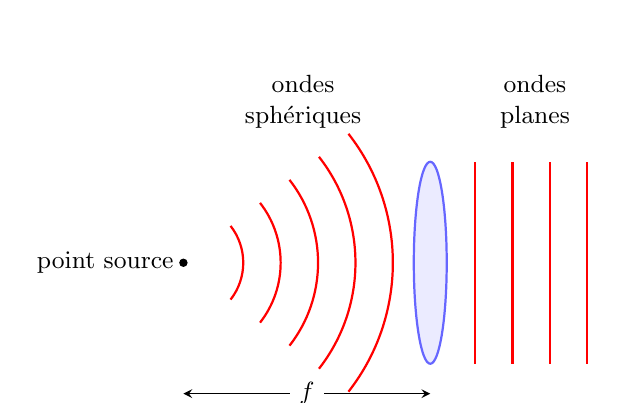
\begin{tikzpicture}[>=stealth,scale=0.95]
    \fill (0,0) circle (1.6pt);
    \node[left,font=\small] at (0,0) {point source};
    \foreach \r in {0.8,1.3,1.8,2.3,2.8}{
      \draw[red,thick] ({\r*cos(38)},{\r*sin(38)}) arc (38:-38:\r);
    }
    \draw[blue!60,fill=blue!8,thick] (3.3,0) ellipse (0.22 and 1.35);
    \foreach \x in {3.9,4.4,4.9,5.4}{\draw[red,thick] (\x,-1.35) -- (\x,1.35);}
    \draw[<->] (0,-1.75) -- (3.3,-1.75) node[midway,fill=white,font=\small] {$f$};
    \node[font=\small,align=center] at (1.6,2.15) {ondes\\ sphériques};
    \node[font=\small,align=center] at (4.7,2.15) {ondes\\ planes};
  \end{tikzpicture}
  \caption*{\small A lentille convergente as an élément déphasant: the chemin
  optique through the glass is longest on the axis, so the spherical wavefront
  is straightened into a plane one when the source sits at the object focus.}
\end{figure}

\subsection{Expression d'une vibration lumineuse quasi-monochromatique}

Maintenant que l'on dispose de l'expression mathématique d'une onde plane, on
peut se demander quelles sont les fréquences disponibles dans un signal
quelconque et si un outil mathématique pratique existe pour passer du domaine du
temps au domaine des fréquences. Pour un signal périodique, c'est la série de
Fourier. Pour un signal non périodique, cet outil s'appelle la transformée de
Fourier et nous sera très utile en diffraction.

\subsubsection{Rappel : série de Fourier}

Sous certaines conditions de continuité et de dérivation, tout signal périodique
de pulsation $\omega_0$ (ou de fréquence $\nu_0=\omega_0/2\pi$) peut s'écrire
sous la forme d'une somme de cosinus et de sinus, composée d'une
\textbf{composante fondamentale} (\textit{fundamental component}) de fréquence
$\nu_0$ (ou 1ère harmonique) et de différentes \textbf{harmoniques}
(\textit{harmonics}) de fréquences multiples $n\nu_0$ :

\[
  f_{\text{périodique}}(t)=A_0+\sum_{n=1}^{+\infty}A_n\cos(n\omega t)
    +\sum_{n=1}^{+\infty}B_n\sin(n\omega t),
\]
\[
  A_0=\langle f(t)\rangle=\frac{1}{T}\int_{t_0}^{t_0+T}f(t)\,dt,
  \qquad
  A_n=\frac{2}{T}\int_{t_0}^{t_0+T}f(t)\cos(n\omega t)\,dt,
  \qquad
  B_n=\frac{2}{T}\int_{t_0}^{t_0+T}f(t)\sin(n\omega t)\,dt .
\]

Le coefficient $A_0$ est la valeur moyenne de $f(t)$ ($B_0$ n'existe pas, la
valeur moyenne d'un signal impair étant nulle). $A_n$ picks out the even part of
the signal, $B_n$ the odd part.

\begin{remark}
  On peut d'ores et déjà remarquer que les coefficients $A_n$ et $B_n$ ne
  dépendent que de la forme du signal sur une \emph{seule} période ! This
  innocuous remark is what makes the limit $T\to\infty$ work.
\end{remark}

Le cosinus déphasé peut s'exprimer encore plus simplement sous forme de somme
d'exponentielles complexes. De fait, en toute généralité, une vibration
quelconque peut s'écrire comme la somme d'une infinité continue ou discrète de
composantes oscillantes monochromatiques :

\[
  f_{\text{périodique}}(t)=A_0+\sum_{n\neq 0}C_ne^{jn\omega t},
  \qquad
  C_n=\frac{1}{2}\left(A_n-jB_n\right)=\frac{1}{T}\int_{t_0}^{t_0+T}f(t)e^{-jn\omega t}\,dt .
\]

\begin{notation}[$i$ or $j$]
  The sections on ondes use $i$; from the Fourier sections onwards the
  engineering $j$ mostly takes over, though $i$ reappears in the translation
  property, $TF[f(t-\tau)]=e^{-2i\pi\nu\tau}F[\nu]$. The two are the same
  imaginary unit, and the appendix table is written with $j$.
\end{notation}

\begin{remark}[The analysis kernel]
  The kernel that analyses is the conjugate of the one that synthesises: the
  synthesis sum carries $e^{+jn\omega t}$ and the analysis integral
  $e^{-jn\omega t}$, consistently with $C_n=\frac{1}{2}(A_n-jB_n)$. The passage
  to the transformée de Fourier below writes the same integral as
  $C_nT=\int f(t)e^{-j\omega t}dt$, and the transform itself as
  $e^{-2j\pi\nu t}$: the minus sign belongs to the transformée directe.
\end{remark}

\subsubsection{Illustration sur un signal périodique de forme carrée}

Pour illustrer la série de Fourier, analysons un signal périodique de forme
carrée. Le signal étant centré autour de 0, la valeur moyenne du signal est nulle
($A_0=0$). Whether the square is taken \emph{even} --- the $B_n$ then vanish and
the $A_n$ (cosine) formula applies --- or \emph{odd}, as drawn below (un signal
périodique carré impair, built from $A_n\sin 2\pi\nu_nt$), the two readings
differ only by the choice of time origin, and the amplitudes are the same either
way:

\[
  A_1=1{,}27,\quad A_3=0{,}42,\quad A_5=0{,}25,\quad A_7=0{,}18,
  \quad A_9=0{,}14,\quad A_{11}=0{,}12 .
\]

Avec uniquement la composante fondamentale, on constate que l'ajustement est
grossier. Son amplitude permet de représenter la variation du signal (contraste),
et sa période est la même que le signal carré à approximer. Par contre, le signal
résultant est parfois au-dessus du signal initial ou au-dessous, avec trois
alternances sur la période --- three times in excess and three times in deficit.
Il convient donc d'ajouter une harmonique de fréquence triple de l'harmonique
fondamental qui va permettre d'ajouter le manque dans les zones en déficit et de
retrancher le surplus dans les zones en excès. On constate cependant une
nouvelle fois des zones en excès et des zones en manque, cette fois à une
fréquence $5\nu_0$ : il est donc nécessaire d'ajouter un harmonique d'amplitude
$A_5$. Le raisonnement peut se poursuivre à l'infini.

\begin{figure}[h!]
  \centering
  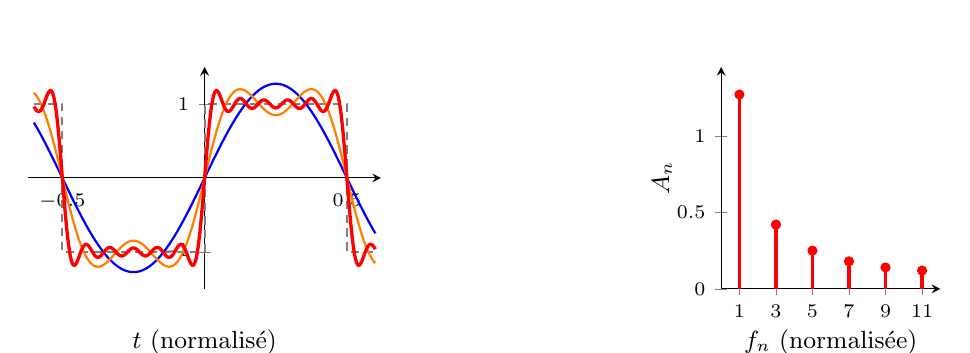
\begin{tikzpicture}
    \begin{axis}[
      width=0.50\textwidth, height=4.4cm,
      axis lines=middle, xmin=-0.62, xmax=0.62, ymin=-1.5, ymax=1.5,
      xtick={-0.5,0.5}, ytick={-1,1},
      xlabel={$t$ (normalisé)}, tick label style={font=\scriptsize},
      every axis x label/.style={at={(axis description cs:0.5,-0.14)},anchor=north,font=\small},
      ]
      \addplot[gray,thick,densely dashed] coordinates
        {(-0.6,1)(-0.5,1)(-0.5,-1)(0,-1)(0,1)(0.5,1)(0.5,-1)(0.6,-1)};
      \addplot[blue,thick,domain=-0.6:0.6,samples=300]
        {1.2732*sin(deg(2*pi*x))};
      \addplot[orange,thick,domain=-0.6:0.6,samples=400]
        {1.2732*sin(deg(2*pi*x))+0.4244*sin(deg(6*pi*x))};
      \addplot[red,very thick,domain=-0.6:0.6,samples=600]
        {1.2732*sin(deg(2*pi*x))+0.4244*sin(deg(6*pi*x))+0.2546*sin(deg(10*pi*x))
         +0.1819*sin(deg(14*pi*x))+0.1415*sin(deg(18*pi*x))+0.1157*sin(deg(22*pi*x))};
    \end{axis}
    \begin{scope}[xshift=8.8cm]
    \begin{axis}[
      width=0.36\textwidth, height=4.4cm,
      axis lines=left, xmin=0, xmax=12, ymin=0, ymax=1.45,
      xtick={1,3,5,7,9,11}, ytick={0,0.5,1},
      xlabel={$f_n$ (normalisée)}, ylabel={$A_n$},
      tick label style={font=\scriptsize},
      every axis x label/.style={at={(axis description cs:0.5,-0.14)},anchor=north,font=\small},
      every axis y label/.style={at={(axis description cs:-0.18,0.5)},rotate=90,anchor=south,font=\small},
      ]
      \addplot[ycomb,red,very thick,mark=*,mark size=1.2pt] coordinates
        {(1,1.27)(3,0.42)(5,0.25)(7,0.18)(9,0.14)(11,0.12)};
    \end{axis}
    \end{scope}
  \end{tikzpicture}
  \caption*{\small Left: the square signal (dashed) and its partial sums with
  $1$, $2$ and $6$ harmoniques. Right: the amplitude spectrum --- discrete, a
  spectre de raies, because the signal is periodic.}
\end{figure}

\begin{conclusion}[What to keep from the Fourier series]
  Le coefficient $A_0$ représente la valeur moyenne du signal. Les basses
  fréquences ne donnent qu'une idée grossière (« floue ») de la fonction créneau
  alors que les hautes fréquences permettent d'en préciser les contours --- its
  rising edges, its details. La composante fondamentale, avec sa grande
  amplitude, permet de représenter la variation du signal (contraste). La
  reconstruction, par une gamme de plus en plus complète d'ondes sinusoïdales de
  fréquences croissantes, aboutit ainsi à une représentation de plus en plus
  fidèle du signal. On verra qu'il en sera de même pour représenter, sur une
  image, les contours d'une zone de variation d'intensité de signal. Dans le cas
  d'un signal périodique, le spectre qui représente les amplitudes des
  harmoniques en fonction de la fréquence est \emph{discret}, c'est un
  \textbf{spectre de raies} (\textit{line spectrum}).
\end{conclusion}

D'un point de vue plus pratique, l'analyse spectrale d'un signal audio
enregistré par un microphone : si le signal est périodique, le spectre dans
l'espace fréquentiel est discret. Une série de filtres sur l'égaliseur de votre
chaîne HIFI permet alors d'amplifier ou d'atténuer les différentes fréquences
(basses ou aiguës).

\begin{remark}
  Lorsque l'on décompose la série de Fourier en exponentielles, on voit
  apparaître des \textbf{fréquences négatives} (\textit{negative frequency}).
  Celles-ci n'ont pas d'existence réelle mais elles doivent participer au calcul
  lors de la reconstruction du signal.
\end{remark}

\subsubsection{De la série de Fourier à la transformée de Fourier}

En pratique, le signal n'est pas toujours périodique. The transformée de Fourier
is the limiting case of the Fourier series when the signal is not periodic. C'est
naturel puisqu'on peut considérer qu'un signal non périodique est en fait
périodique de période \emph{infinie} !

\paragraph{Illustration pratique.} On considère un signal périodique carré, dont
le motif élémentaire garde une durée $t_0=1$ ms mais dont la période $T_0$
augmente. The elementary pattern is a porte, and the duty cycle falls from
$25\%$ to $0{,}1\%$:

\begin{center}
  \small
  \begin{tabular}{lcccc}
    \toprule
    $T_0$ & 4 ms & 20 ms & 100 ms & 1 s \\
    duty cycle & $25\%$ & $5\%$ & $1\%$ & $0{,}1\%$ \\
    $\nu_0=1/T_0$ & 0,25 kHz & 0,05 kHz & 0,01 kHz & 0,001 kHz \\
    first zero of the envelope & \multicolumn{4}{c}{$1/t_0=1$ kHz, unchanged}\\
    \bottomrule
  \end{tabular}
\end{center}

On constate clairement que si $T_0$ augmente, l'enveloppe des différents
harmoniques reste inchangée. C'est normal puisque les coefficients ne dépendent
que du motif périodique (qui reste ici inchangé). Et la différence entre deux
points de la série de Fourier est $\Delta\nu=(n+1)\nu_0-n\nu_0=\nu_0=1/T_0$ :
c'est tout simplement la fréquence fondamentale. La séparation entre les
harmoniques devient donc de plus en plus petite. Quand $T_0\to\infty$, on passe
d'un spectre qui est seulement défini à quelques points (spectre de raies) à un
spectre composé d'une infinité d'harmoniques, un \textbf{spectre continu}
(\textit{continuous spectrum}). Ce spectre continu fournit donc toutes les
fréquences disponibles dans le motif non périodique, comme le faisait la série
de Fourier pour le signal périodique.

\paragraph{Mathématiquement.} Un signal périodique peut s'écrire en insérant
l'expression de $C_n$ dans la série :

\[
  f_T(t)\propto\sum_{n=-\infty}^{+\infty}
    \left[\nu\int_{-T/2}^{T/2}f(t')e^{-2j\pi n\nu t'}dt'\right]e^{2j\pi n\nu t},
\]

faisons tendre $T\to\infty$, c'est-à-dire $\nu\to 0$. On reconnaît ici une
intégrale au sens de Riemann, c'est-à-dire l'aire sous la courbe. Lorsque
$T\to\infty$ : la séparation entre les harmoniques devient de plus en plus
petite, $\Delta\nu\to d\nu$ ; on passe d'un spectre discret à un spectre
continu ; $n\nu_0\to\nu$ ; enfin, les coefficients $C_n$ de la série de Fourier
deviennent de plus en plus faibles, $C_n\to 0$. Cependant, le produit $C_nT$ ne
devient pas nul. Il représente le spectre, qui est cette fois continu :

\[
  C_nT=\int_{-\infty}^{+\infty}f(t)e^{-j\omega t}\,dt=\hat{F}(\nu).
\]

\begin{definition}[Transformée de Fourier (\textit{Fourier transform})]
  \[
    \boxed{\;\hat{F}(\nu)=TF[f(t)]=\int_{-\infty}^{+\infty}f(t)\,e^{-2j\pi\nu t}\,dt\;}
    \qquad
    \boxed{\;f(t)=TF^{-1}[\hat{F}(\nu)]=\int_{-\infty}^{+\infty}\hat{F}(\nu)\,e^{+2j\pi\nu t}\,d\nu\;}
  \]
  On a étendu les bornes de l'intégrale car $f(t)$ est considérée comme bornée.
\end{definition}

\begin{notation}[Conventions to keep exactly]
  The $2\pi$ sits \emph{inside} the exponent, paired with the frequency $\nu$
  and not with the pulsation $\omega$; there is therefore \emph{no} $1/2\pi$
  prefactor anywhere. The \textbf{transformée directe} (\textit{direct
  transform}) carries the \emph{minus} sign, the \textbf{transformée de Fourier
  inverse} (\textit{inverse Fourier transform}) the plus. The appendix table of
  transforms is written in exactly this convention.
\end{notation}

En d'autres termes, un signal temporel non périodique est la somme continue
d'harmoniques $e^{+2j\pi\nu t}$ de différentes fréquences dont les amplitudes
respectives sont représentées par le spectre continu $\hat F(\nu)$. On peut
aussi dire que tout signal temporel non périodique peut se décomposer sur une
base d'ondes planes de fréquence variable $e^{+2j\pi\nu t}$. En résumé, faire la
TF d'un signal, c'est se poser la question : « quelles sont les composantes
fréquentielles disponibles dans ce signal et quelles sont leurs amplitudes
respectives ? » La TF joue le même rôle que les coefficients de Fourier $C_n$
d'un signal périodique. Pour obtenir le spectre d'une source, il suffit
d'effectuer une transformée de Fourier du signal analytique temporel.
Inversement, pour obtenir l'allure temporelle de la vibration, il suffit
d'effectuer une transformée de Fourier inverse du spectre fréquentiel en
amplitude.

\begin{remark}
  Pour que la transformée de Fourier existe, il faut que la fonction $f(t)$
  converge (condition nécessaire mais pas suffisante). Pour les fonctions qui ne
  convergent pas (une constante par exemple), une gymnastique mathématique est
  nécessaire, vous la verrez en cours de mathématique. Les TF peuvent
  exister dans d'autres domaines duaux que le temps et la fréquence, c'est ce
  que nous verrons en diffraction.
\end{remark}

\subsubsection{Notion d'espaces duaux}

\begin{definition}[Espaces duaux]
  Dans notre exemple, la TF permet de passer de l'espace des « temps » à
  l'espace des « fréquences ». On dit qu'il s'agit des deux \textbf{espaces
  duaux} (\textit{dual space}) de la TF : temps et fréquence.
\end{definition}

On verra qu'en diffraction, la TF nous permettra de passer de l'espace des
« dimensions » à l'espace des vecteurs d'onde $\v{k}$, donc des directions, que
l'on appellera par analogie \textbf{fréquences angulaires} (\textit{angular
frequency}). The spatial pair is written $(x,y)\lra(u,v)$, $u$ and $v$ being the
\textbf{fréquences spatiales} (\textit{spatial frequency}), and the appendix
table gives that pair as

\[
  F(x,y)=\iint f(u,v)\,e^{-2j\pi(ux+vy)}\,du\,dv,
  \qquad
  f(u,v)=\iint F(x,y)\,e^{+2j\pi(ux+vy)}\,dx\,dy .
\]

\begin{remark}
  The two readings of the appendix table are not parallel, and this is where
  signs get lost. In the temporal reading the minus sign goes with the
  transform \emph{towards} the frequency variable; in the spatial reading the
  appendix assigns the lower-case variable to $u$ and the upper-case one to $x$,
  so the minus sign goes with the transform \emph{towards} the space variable.
  The entry read left-to-right off the table is a $u\to x$ pair, not an
  $x\to u$ one.
\end{remark}

\subsubsection{Quelques propriétés élémentaires de la TF}

La transformée de Fourier, ou plus généralement l'analyse fréquentielle ou
spectrale, est un outil fondamental pour la compréhension et la mise en œuvre de
nombreuses techniques numériques de traitement des signaux et des images. On la
trouve dans des applications directes comme l'analyse harmonique des vibrations
et des signaux musicaux, mais aussi dans des domaines très variés. On peut citer
toutes les applications où il est nécessaire de mettre en forme les signaux
mesurés par des capteurs grâce à un filtrage. On l'utilise dans le codage à débit
réduit de la musique et de la parole, la reconnaissance vocale, l'amélioration de
la qualité des images, leur compression, les transmissions numériques, les
nouveaux systèmes de radiodiffusion et de télédiffusion, dans les applications
biomédicales (scanner, imagerie par résonance magnétique nucléaire), en
astronomie (synthèse d'image par interférométrie), en modélisation de
propagation d'ondes, en analyse spectrale pour l'étude de structures
moléculaires ainsi qu'en cristallographie. Son extension (calculs sur les corps
finis) est utilisée dans les méthodes de correction d'erreurs en transmission
numérique. Elle intervient aussi dans les méthodes envisagées en informatique
quantique pour la factorisation de nombres.

\begin{prop}[Linéarité (\textit{linearity})]
  La TF d'une somme de deux fonctions est la somme de leur TF respective.
\end{prop}

\begin{prop}[Changement d'échelle (\textit{change of scale})]
  \[
    TF[f(at)]=\frac{1}{|a|}F\!\left(\frac{\nu}{a}\right).
  \]
  Si on dilate / contracte les coordonnées dans l'espace direct, on observe
  inversement une contraction / dilatation de l'espace spectral et un
  changement de l'amplitude du spectre.
\end{prop}

Cette propriété permet de déduire la transformée de Fourier de bon nombre de
fonctions ou de distributions à partir de leur TF de base qui vous sont fournies
dans un tableau en annexe. C'est une propriété que l'on connaît finalement tous
sans l'énoncer : chacun sait que plus la période d'un sinus est grande, plus sa
fréquence est petite et vice versa.

\begin{remark}
  Certains connaissent déjà cette propriété à travers l'inégalité de Heisenberg,
  affirmant qu'il existe une limite fondamentale à la précision avec laquelle il
  est possible de connaître simultanément deux propriétés physiques d'une même
  particule : la position $x$ et sa quantité de mouvement $p$. Ce principe est
  une conséquence mathématique de la dualité onde-corpuscule de la matière et de
  la représentation des corpuscules sous forme de paquet d'onde selon une
  distribution de fréquences (un spectre) ou une distribution de positions dans
  l'espace. Le passage de l'un à l'autre se calcule par une transformée de
  Fourier.
\end{remark}

\begin{prop}[Translation ou déphasage (\textit{translation or dephasing})]
  Une translation de la fonction $f(t)$ d'un temps $\tau$ se traduit par un
  déphasage du spectre dans le domaine des fréquences :
  \[
    TF[f(t-\tau)]=e^{-2i\pi\nu\tau}F[\nu].
  \]
  Réciproquement, un déphasage de la fonction temporelle provoque une
  translation en fréquence du spectre.
\end{prop}

\begin{theorem}[Théorème de Parseval-Plancherel (\textit{Parseval--Plancherel theorem})]
  \[
    \int|f(t)|^2\,dt=\int|\hat{F}(\nu)|^2\,d\nu .
  \]
\end{theorem}

Ces deux intégrales sont proportionnelles à l'énergie du signal contenue dans
$f(t)$ ou $\hat F(\nu)$. Ceci traduit le fait que l'on peut mesurer la puissance
dans les deux domaines et que l'on doit trouver la même valeur. Ceci explique le
facteur $1/|a|$ dans l'expression du changement d'échelle, c'est en fait un
facteur de conservation d'énergie. L'intégrale du second membre de l'équation
correspond à une décomposition en vibrations harmoniques. Elle exprime le fait
que l'énergie totale est la somme des énergies de chacune des composantes. Cette
relation a été utilisée pour la première fois par un physicien (Lord Rayleigh,
1889).

\subsubsection{Quelques TF de distributions usuelles}

Le but de cette partie n'est pas de faire un cours de math exhaustif --- la
notion de distribution ne sera pas développée ici. Le but est seulement de donner
quelques outils essentiels à la résolution de certains exercices. C'est plutôt le
sens \emph{physique} de ces outils mathématiques qu'il sera intéressant de mettre
en évidence. Il est surtout intéressant de noter que la définition de la
transformée de Fourier peut s'étendre au cas des distributions.

\paragraph{Distribution « porte ».} La fonction porte est essentielle en théorie
du signal. Elle permet par exemple d'effectuer des troncatures temporelles. En
optique, elle nous permet de représenter des fentes, de limiter la taille des
ouvertures, etc.

\begin{definition}[Porte (\textit{gate})]
  Les définitions de la porte unité et d'une porte de largeur $A$ sont :
  \[
    \boldsymbol{\pi}(t)=\begin{cases}1 & \text{si } |t|<\tfrac12\\ 0 & \text{sinon}\end{cases}
    \qquad\qquad
    \boldsymbol{\pi}_A(t)=\boldsymbol{\pi}\!\left(\frac{t}{A}\right)
      =\begin{cases}1 & \text{si } |t|<\tfrac{A}{2}\\ 0 & \text{sinon}\end{cases}
  \]
  so that $A$ is the \emph{total} width, not the half-width.
\end{definition}

\begin{prop}
  \[
    \boldsymbol{\pi}_A(t)\ \xleftrightarrow{\ TF\ }\
    s(\nu)=A\,\frac{\sin\pi\nu A}{\pi\nu A}=A\sinc(\pi\nu A),
  \]
  une fonction en sinus cardinal, continue, whose first zeros sit at
  $\nu=\pm 1/A$.
\end{prop}

Le spectre d'un signal temporel de forme carrée, \emph{non périodique}, est une
fonction en sinus cardinal. Il correspond, comme nous l'avons dit précédemment, à
l'enveloppe des harmoniques de la série de Fourier d'un signal périodique dont le
motif est le même. Note that the $\pi$ is already written into the argument:
the course's $\sinc$ is the unnormalised $\sin x/x$, so feeding it an argument
without the $\pi$ is the quickest way to lose a factor $\pi$.

\begin{figure}[h!]
  \centering
  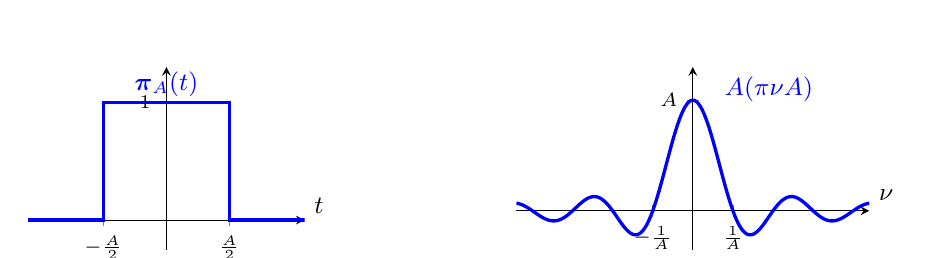
\begin{tikzpicture}
    \begin{axis}[
      width=0.42\textwidth, height=3.9cm,
      axis lines=middle, xmin=-1.1, xmax=1.1, ymin=-0.25, ymax=1.3,
      xtick={-0.5,0.5}, xticklabels={$-\frac{A}{2}$,$\frac{A}{2}$},
      ytick={1}, xlabel={$t$}, tick label style={font=\scriptsize},
      every axis x label/.style={at={(axis description cs:1.0,0.24)},anchor=west,font=\small},
      ]
      \addplot[blue,very thick] coordinates
        {(-1.1,0)(-0.5,0)(-0.5,1)(0.5,1)(0.5,0)(1.1,0)};
      \node[font=\small,blue] at (axis cs:0,1.15) {$\boldsymbol{\pi}_A(t)$};
    \end{axis}
    \begin{scope}[xshift=6.2cm]
    \begin{axis}[
      width=0.50\textwidth, height=3.9cm,
      axis lines=middle, xmin=-4.4, xmax=4.4, ymin=-0.35, ymax=1.3,
      xtick={-1,1}, xticklabels={$-\frac{1}{A}$,$\frac{1}{A}$},
      ytick={1}, yticklabels={$A$}, xlabel={$\nu$},
      tick label style={font=\scriptsize},
      every axis x label/.style={at={(axis description cs:1.0,0.30)},anchor=west,font=\small},
      ]
      \addplot[blue,very thick,domain=-4.4:4.4,samples=400]
        {sin(deg(pi*x))/(pi*x)};
      \node[font=\small,blue] at (axis cs:1.9,1.1) {$A\sinc(\pi\nu A)$};
    \end{axis}
    \end{scope}
  \end{tikzpicture}
  \caption*{\small A porte of total width $A$ and its transform, a cardinal
  sine of amplitude $A$ whose first zeros are at $\pm 1/A$. Narrowing the porte
  widens the sinc --- the changement d'échelle property.}
\end{figure}

\paragraph{Exemple intuitif : TF d'une fonction sinusoïdale infinie.} Si on
reprend le cas d'une onde plane monochromatique --- that of the first half of
the chapter --- au sens temporel du terme, représentable par un cosinus de durée
infinie, et si l'on se pose la question : « dans un cosinus $\cos(2\pi t/T_0)$
temporellement infini, combien y a-t-il de fréquences ? », l'étudiant répondra
naturellement qu'il n'y en a qu'une seule et qu'elle vaut $\nu=1/T_0$. Il aura
fait sans le savoir une transformée de Fourier :

\[
  V(t)=\cos\omega_0t=\cos 2\pi\nu_0t=\frac{1}{2}\left(e^{2j\pi\nu_0t}+e^{-2j\pi\nu_0t}\right)
  \ \xleftrightarrow{\ TF\ }\
  s(\nu)=\frac{1}{2}\left[\delta(\nu+\nu_0)+\delta(\nu-\nu_0)\right],
\]

où $\delta(\nu\pm\nu_0)$ représente une distribution de Dirac centrée en
$\mp\nu_0$. $s(\nu)$ est le spectre en amplitude, et

\[
  S(\nu)=|s(\nu)|^2
\]

est la \textbf{densité spectrale de puissance} (\textit{power spectral density})
de l'onde. Par définition, le \textbf{spectre électromagnétique}
(\textit{electromagnetic spectrum}) est la décomposition du rayonnement
électromagnétique selon ses différentes composantes en termes de fréquence ou
encore de longueur d'onde associée. Plus précisément, le spectre $S(\nu)$ est la
densité spectrale de puissance.

\begin{conclusion}
  Le spectre en amplitude d'une onde prenant la forme d'un cosinus de durée
  infinie est bien monochromatique, c'est-à-dire qu'il ne comprend qu'une et une
  seule fréquence (ou longueur d'onde).
\end{conclusion}

\begin{remark}[Fréquences négatives]
  La notion de fréquence négative n'a pas de réalité physique. Elles
  apparaissent lorsque l'on utilise les mathématiques pour comprendre la
  physique ! En effet, lorsque l'on développe $\cos 2\pi\nu_0t$ en exponentielles
  complexes, on voit apparaître des termes en $e^{2j\pi\nu_0t}$ et
  $e^{-2j\pi\nu_0t}$. On comprend à travers ces deux expressions que si
  $2\pi\nu_0$ est positif, alors, artificiellement, $-2\pi\nu_0$ devient
  négatif. Lors d'une interprétation physique, on n'oubliera pas de supprimer la
  partie négative du spectre : the two-line spectrum above is the
  \textbf{spectre mathématique} (\textit{mathematical spectrum}), the single
  line at $+\nu_0$ the \textbf{spectre physique} (\textit{physical spectrum}).
  Vu autrement, on peut aussi dire que pour un signal réel, nous aurons
  nécessairement $s(\nu)=s^{*}(-\nu)$ et que l'on peut donc se restreindre aux
  fréquences positives pour analyser complètement un signal puisque toute
  l'information y est contenue.
\end{remark}

\begin{notation}
  Dans les calculs, à partir de maintenant, on représentera une vibration par
  son signal analytique $V(t)$. Si les opérations sur $V(t)$ sont linéaires, on
  fera les calculs avec $V(t)$ puis on prendra la partie réelle $V_r(t)$ à la
  fin des calculs pour en déduire la vibration réelle et pouvoir ainsi faire une
  interprétation physique du phénomène observé. A general signal is then read
  as
  \[
    V(t)=\int_{-\infty}^{+\infty}\underbrace{s(\nu)}_{\text{amplitude of each component}\,\equiv\,\text{spectrum}}
      \underbrace{e^{2j\pi\nu t}}_{\text{term oscillating at }\nu\ \equiv\ \text{plane wave}}d\nu .
  \]
\end{notation}

\paragraph{Distribution de Dirac.}

\begin{definition}[Distribution de Dirac (\textit{Dirac distribution})]
  La distribution de Dirac $\delta(t)$ peut être définie comme une porte dont la
  largeur tendrait vers 0 tandis que sa hauteur tendrait vers l'infini de telle
  sorte que son aire, que l'on appelle également son \textbf{poids}
  (\textit{weight}), reste égale à $1$ :
  \[
    \delta(t)=\lim_{\varepsilon\to 0}\frac{1}{\varepsilon}\boldsymbol{\pi}_\varepsilon(t)
             =\lim_{\varepsilon\to 0}\frac{1}{\varepsilon}\boldsymbol{\pi}\!\left(\frac{t}{\varepsilon}\right).
  \]
\end{definition}

Cet objet mathématique représente en optique un point lumineux de taille
négligeable dans le domaine spatial, une impulsion de lumière infiniment courte
dans le domaine temporel ou encore une émission parfaitement monochromatique dans
le domaine spectral. Le Dirac revêt un aspect purement théorique et n'a pas de
sens physique on its own: un trou infiniment fin ne laisse pas passer de
lumière ! En optique, de surcroît, lorsque l'on fait tendre une porte vers une
largeur nulle, sa transmittance ne tend pas vers l'infini mais garde la même
valeur ! Ceci dit, lorsqu'on \emph{convolue} un Dirac avec une fonction,
c'est-à-dire en accord avec les lois de la physique (dérivable à dérivée
continue), le résultat est physique. La convolution sera abordée au chapitre
suivant.\\

Si on calcule la transformée de Fourier, en accord avec la propriété de
changement d'échelle, son extension étant temporellement nulle, l'amplitude de
son spectre sera au contraire infiniment étalée spectralement :

\[
  \delta(t)\ \xleftrightarrow{\ TF\ }\ \mathbf{1}(\nu),
  \qquad\qquad
  TF[\delta(t-\tau)]=\underbrace{e^{-2j\pi\nu\tau}}_{\text{dephasing}} .
\]

\begin{remark}
  The sign of the second relation is the one the translation property,
  $TF[f(t-\tau)]=e^{-2i\pi\nu\tau}F[\nu]$, and the appendix entry
  $\delta(\xi-\xi_0)\lra\exp(-2j\pi\xi_0\Xi)$ both give. A translation is a
  pure dephasing, of unit modulus, but its sign matters as soon as two such terms
  interfere.
\end{remark}

\begin{remark}
  On n'oubliera pas la flèche sur le Dirac quand on le représente sur un
  graphe. Cela montre qu'on ne représente pas son amplitude (qui est infinie)
  mais son aire (ou son poids).
\end{remark}

\paragraph{Distribution peigne de Dirac.}

\begin{definition}[Peigne de Dirac (\textit{Dirac comb})]
  Un ensemble d'impulsions de Dirac régulièrement espacées, d'expression
  analytique :
  \[
    \boldsymbol{\omega}_\tau(t)=\sum_{n=-\infty}^{+\infty}\delta(t-n\tau).
  \]
\end{definition}

On verra dans le chapitre suivant que l'on utilise souvent cette distribution
dans le cas de fonctions périodiques mais qu'elle n'a pas plus de sens physique
qu'un Dirac seul. On montre que le spectre d'un peigne de Dirac est également un
peigne de Dirac dont le pas a changé :

\[
  \boldsymbol{\omega}_\tau(t)=\sum_{n=-\infty}^{+\infty}\delta(t-n\tau)
  \ \xleftrightarrow{\ TF\ }\
  \frac{1}{\tau}\,\boldsymbol{\omega}_{1/\tau}(\nu)
  =\frac{1}{\tau}\sum_{n=-\infty}^{+\infty}\delta\!\left(\nu-\frac{n}{\tau}\right).
\]

\begin{remark}
  Le terme en $1/\tau$ devant les Diracs dans le domaine de Fourier peut être
  interprété comme un terme de conservation de l'énergie pour satisfaire au
  théorème de Parseval-Plancherel. It is the factor most often dropped. Beware
  also of mixing letters when transcribing from the appendix table, which names
  the step $L$ and the frequency $\Xi$: for the peigne de Dirac above the
  prefactor is $1/\tau$ and the teeth are $\delta(\nu-n/\tau)$.
\end{remark}

\begin{figure}[h!]
  \centering
  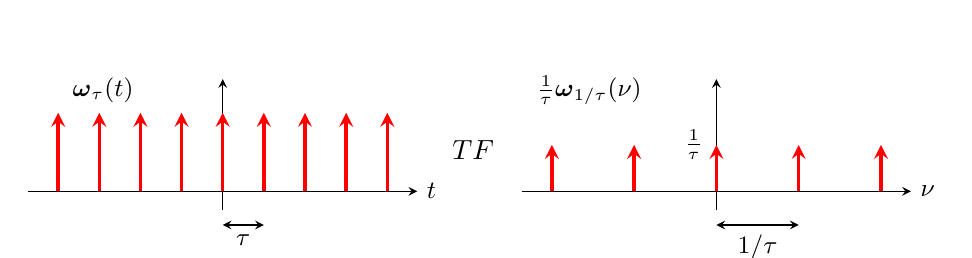
\begin{tikzpicture}[>=stealth,scale=0.95]
    \draw[->] (-2.6,0) -- (2.6,0) node[right,font=\small] {$t$};
    \draw[->] (0,-0.25) -- (0,1.5);
    \foreach \n in {-4,-3,-2,-1,0,1,2,3,4}{
      \draw[->,red,very thick] (\n*0.55,0) -- (\n*0.55,1.05);}
    \node[font=\small] at (-1.6,1.35) {$\boldsymbol{\omega}_\tau(t)$};
    \draw[<->] (0,-0.45) -- (0.55,-0.45) node[midway,below,font=\small] {$\tau$};
    \node at (3.35,0.55) {$\xleftrightarrow{\ TF\ }$};
    \begin{scope}[xshift=6.6cm]
      \draw[->] (-2.6,0) -- (2.6,0) node[right,font=\small] {$\nu$};
      \draw[->] (0,-0.25) -- (0,1.5);
      \foreach \n in {-2,-1,0,1,2}{
        \draw[->,red,very thick] (\n*1.1,0) -- (\n*1.1,0.62);}
      \node[font=\small] at (-1.7,1.35) {$\frac{1}{\tau}\boldsymbol{\omega}_{1/\tau}(\nu)$};
      \draw[<->] (0,-0.45) -- (1.1,-0.45) node[midway,below,font=\small] {$1/\tau$};
      \node[left,font=\small] at (-0.05,0.62) {$\frac{1}{\tau}$};
    \end{scope}
  \end{tikzpicture}
  \caption*{\small A peigne de Dirac of step $\tau$ and unit poids transforms
  into a peigne of step $1/\tau$ and poids $1/\tau$: tighten the teeth in time
  and they spread in frequency.}
\end{figure}

\subsubsection{Conséquence d'une troncature temporelle d'une onde monochromatique sur son spectre}

Si une vibration temporellement infinie correspond à un spectre monochromatique
par transformée de Fourier, il n'y a aucune raison pour qu'en \emph{tronquant}
temporellement cette onde lumineuse, sa TF reste une distribution de Dirac !\\

Or, le processus d'émission de lumière fait que les atomes n'émettent que
pendant un temps limité $\tau$, qui correspond à la durée de vie des états
excités dans la théorie quantique et au coefficient d'amortissement dans la
théorie classique. Une onde n'est donc jamais infinie temporellement !

\begin{conclusion}
  La conséquence d'une troncature temporelle d'une onde due au processus
  d'émission de la lumière est donc que son spectre n'est plus monochromatique.
  Il contient d'autres fréquences que la fréquence centrale. En pratique, c'est
  plus ou moins le cas suivant le type de source mais c'est toujours le cas.
  \textbf{Il n'existe pas de source parfaitement monochromatique} !
  Inversement, la conséquence du fait qu'une source ne soit jamais purement
  monochromatique est que les trains d'onde n'ont jamais une durée (ou une
  longueur) infinie.
\end{conclusion}

\subsection{Formules de Fresnel}

A complement, not developed in the rest of this chapter, whose conclusion is
used in the fibre chapter. For an onde incident at angle $i$ on a dioptre
between indices $n_1$ and $n_2$, refracted at $i'$, the amplitude reflection and
transmission coefficients split by polarisation --- $\parallel$ for the field in
the plane of incidence, $\perp$ for the field normal to it:

\[
  r_{\parallel}=-\frac{\tan(i-i')}{\tan(i+i')},\qquad
  t_{\parallel}=\frac{2\cos i\,\sin i'}{\sin(i+i')\cos(i-i')},\qquad
  r_{\perp}=-\frac{\sin(i-i')}{\sin(i+i')},\qquad
  t_{\perp}=\frac{2\cos i\,\sin i'}{\sin(i+i')} .
\]

\begin{conclusion}
  Le déphasage à la réflexion est $\pi$ (signe (-)) tant que l'on ne se trouve
  pas en réflexion totale. Dans le cas de la réflexion totale, ce déphasage est
  beaucoup plus compliqué et dépend à la fois de la polarisation et de l'angle
  d'incidence. Phénomène important dans la fibre optique !
\end{conclusion}

\section{Diffraction}
L'optique géométrique ne suffit pas ! En regardant un réverbère la nuit à
travers le rideau d'une fenêtre, on voit autour du point lumineux central une
croix, éventuellement colorée, dont les bras sont perpendiculaires aux fils de
la toile du rideau. Lors de son passage à travers les petits trous du tissu, la
lumière est déviée par rapport à la propagation rectiligne prédite par
l'optique géométrique. Ceci n'est pas dû à la réfraction. On peut également
observer un phénomène de même nature à l'entrée d'un port où les vagues
provenant de la mer (onde plane) se retrouvent limitées spatialement par
l'entrée de ce dernier. On voit alors l'onde plane se transformer en première
approximation en onde circulaire.

Des phénomènes analogues d'\textbf{éparpillement} (\textit{spreading}) de la
lumière apparaissent dès qu'une onde lumineuse est spatialement limitée par un
obstacle matériel --- this is \textbf{diffraction}. La répartition de la
lumière dans l'espace, en dehors du chemin optique géométrique, dépend de la
forme géométrique limitante (bord d'écran, fente rectangulaire, trou
circulaire). Ce phénomène de diffraction joue un rôle décisif dans la formation
des images puisque tout système d'optique limite irrémédiablement l'étendue de
l'onde incidente à commencer par notre outil d'observation : l'œil.

\begin{remark}
  Not every coloured optical effect is diffraction. A rainbow is refraction plus
  dispersion; the colours of a soap bubble are thin-film interference. What
  identifies diffraction is that the light has been spatially limited.
\end{remark}

Une interprétation des phénomènes de diffraction, observés en premier par
l'italien F. Grimaldi vers 1660, avait été fournie bien avant Maxwell (1865) par
Huygens (1678) et Fresnel (1818). Pour analyser cette répartition lumineuse, il
faut résoudre les équations de Maxwell en introduisant les conditions aux
limites imposées par l'obstacle. C'est un problème mathématique très compliqué,
qui n'apporte rien à la compréhension de la physique du phénomène.
L'interprétation de Huygens et Fresnel repose sur le principe appelé en
conséquence Huygens-Fresnel. Un outil mathématique puissant, la transformée de
Fourier, permet de réduire à quelques lignes les calculs historiquement longs et
fastidieux.

\begin{remark}
  Les phénomènes de diffraction ne se limitent pas à l'optique mais sont
  observables dans de nombreux autres domaines où des ondes sont mises en jeu :
  ondes radiofréquences (dont la seule différence avec l'optique est la gamme de
  fréquence) et acoustiques, rayons X, mais aussi ondes en mécanique ondulatoire
  associées aux différentes particules matérielles.
\end{remark}

\subsection{Principe de Huygens-Fresnel}

\subsubsection{Résolution par les équations de Maxwell}
Three simplifications justify abandoning the vector treatment. Nous nous
placerons dans le cas d'une ouverture grande devant la longueur d'onde. Dans ce
cas, on considère que l'écran n'apporte aucune perturbation autre que la
suppression des parties masquées, c'est-à-dire que le champ électrique qui passe
à travers l'écran est le même avec ou sans écran. Enfin, si tous les rayons sur
l'écran de diffraction ont une inclinaison faible, les champs diffractés auront
pratiquement la même direction, il n'est alors pas nécessaire de faire
intervenir la direction du champ électrique et la vibration lumineuse peut être
considérée comme une grandeur \textbf{scalaire}. Le principe de Huygens-Fresnel
est alors très efficace et la théorie scalaire dont il est le fondement apparaît
encore à notre époque comme la théorie la plus puissante et la plus adaptée à la
presque totalité des problèmes rencontrés en optique.

\begin{postulate}[Principe de Huygens-Fresnel (\textit{Huygens--Fresnel principle})]
  Si un point $M$ reçoit une onde d'amplitude $E(M,t)$, alors on peut considérer
  que ce point réémet lui-même une onde sphérique de même fréquence, même
  amplitude et même phase que l'onde incidente. Chaque point de l'espace éclairé
  par une onde plane se comporte donc comme une \textbf{source secondaire}
  (\textit{secondary source}) et réémet dans toutes les directions des ondes
  sphériques cohérentes entre elles.
\end{postulate}

Au lieu de considérer que l'onde progresse de manière continue, on décompose sa
progression en imaginant qu'elle progresse de proche en proche. Tous les points
d'une même surface éclairée par une même onde plane, c'est-à-dire spatialement
corrélée et temporellement cohérente, réémettent des ondes cohérentes entre
elles. L'amplitude complexe de la vibration lumineuse en un point de l'espace
$P$ est la somme des amplitudes complexes des vibrations produites par toutes
les sources secondaires. Ces vibrations interfèrent puisqu'elles sont
cohérentes.

\begin{remark}
  On parle de \textbf{cohérence} entre deux ondes quand elles présentent entre
  elles une différence de phase stationnaire. Dans ce cas, les amplitudes
  complexes s'ajoutent mais non les intensités.
\end{remark}

\begin{remark}
  En pratique, l'amplitude rayonnée par chaque onde sphérique n'est pas
  uniforme : anisotropie dans la distribution de l'énergie diffractée, et
  absence de diffraction « arrière ». This is what the facteur d'inclinaison
  below repairs.
\end{remark}

\subsubsection{Hypothèses de départ}
Pour simplifier le problème, nous placerons notre analyse dans le cadre d'une
illumination \textbf{monochromatique} dans un milieu \textbf{linéaire, isotrope,
homogène et permanent}. Les équations de Maxwell étant linéaires, ce qui se
passe pour un éclairement multi-chromatique est la somme \emph{en intensité} de
ce qui se passe à chaque longueur d'onde.

\subsubsection{Étude intuitive de la diffraction}
Prenons $n$ sources ponctuelles émettant dans le plan $(xOy)$ au sens de
Huygens-Fresnel, chacune ayant une amplitude $t_n$ (for the $n$-th). On place à
une distance $D$ un écran d'observation dans le plan $(X,Y)$. Si $D$ tend vers
l'infini, les ondes sphériques émises par l'écran diffractant sont devenues des
ondes planes ! Ainsi, sur l'écran, l'amplitude résultante est la somme de toutes
ces ondes :
\[
  T(X) \propto \sum \left[ t_1 e^{-j\v{k}_1 \cdot \v{r}}
                         + t_2 e^{-j\v{k}_2 \cdot \v{r}} + \cdots \right].
\]
En réalité, il va se former sur l'écran une figure d'interférence, résultat de
la superposition des différentes ondes et de leur déphasage relatif, variable
selon le point d'observation sur l'écran. On va donc observer des zones de
lumière et des zones d'obscurité. Vu la géométrie de l'expérience, on risque de
retrouver dans la figure observée les mêmes symétries que l'objet diffractant.

Si la transmittance de l'écran suivant $(Ox)$ est $t(x)$, éclairée par une onde
plane, l'amplitude des points source diffractés est directement proportionnelle
à $t(x)$. On somme cette fois de façon continue des ondes planes dans le plan
d'observation (intégrale de Riemann) :
\begin{equation*}
  T(X) \propto \int_{-\infty}^{+\infty} t(x)\, e^{-j\v{k}\cdot\v{r}}\, dx .
\end{equation*}
Si on compare à la définition de la transformée de Fourier, on voit clairement
que le champ diffracté est \emph{proportionnel à la transformée de Fourier de
$t(x)$}, c'est-à-dire la TF de l'écran diffractant !

\begin{remark}
  Two things change relative to the temporal transformée de Fourier of the
  previous chapter. Les variables duales de la TF sont cette fois : d'un côté
  l'espace $(x,y)$ (variables d'intégration) ; de l'autre une variable
  proportionnelle à $\v{k}$, c'est-à-dire l'\emph{espace des directions} ! On
  décomposait les signaux temporels sur une base d'harmoniques
  $e^{+j\omega t}$. Ici, on voit que l'on décompose $t(x)$ sur une base d'ondes
  planes $e^{-j\v{k}\cdot\v{r}}$. La convention de signe étant inverse, la TF
  deviendra la TF inverse et réciproquement, ce n'est qu'une histoire de
  convention.
\end{remark}

\begin{notation}
  When the sum is discrete the result is a \textbf{figure d'interférence}
  (\textit{interference pattern}). Lorsque la somme est continue, la figure
  d'interférence s'appelle une \textbf{figure de diffraction}
  (\textit{diffraction pattern}) ! Mais le phénomène est le même : regarder
  l'intensité résultante d'une superposition d'ondes.
\end{notation}

\subsubsection{Étude formelle : amplitude complexe diffractée en un point de l'espace}
Pour connaître l'amplitude complexe de la vibration lumineuse en un point de
l'espace, il suffit de sommer les amplitudes lumineuses complexes de toutes les
ondelettes provenant de l'écran diffractant, avec leur phase accumulée propre
depuis leur émission (écran diffractant) jusqu'au point considéré. Il s'agit
donc, comme tout problème d'interférence, d'un problème géométrique de calcul de
différence de marche.

\begin{figure}[h!]
  \centering
  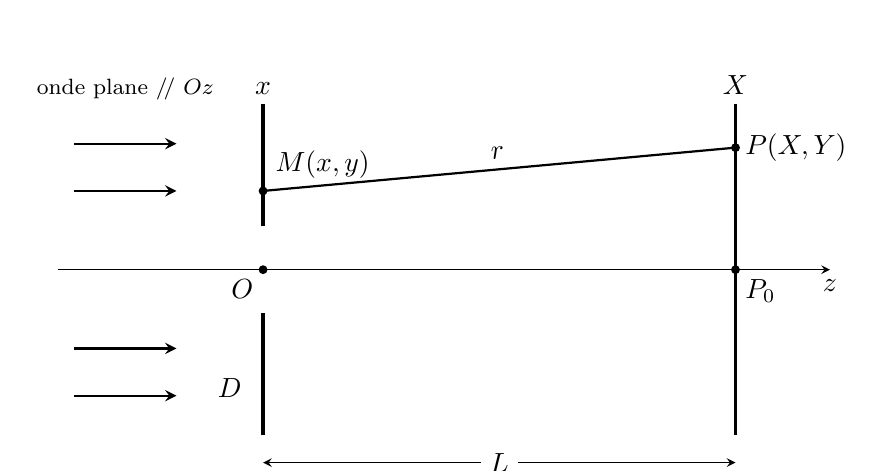
\begin{tikzpicture}[>=stealth, scale=1.0]
    % diffracting screen
    \draw[very thick] (0,-2.1) -- (0,-0.55);
    \draw[very thick] (0,0.55) -- (0,2.1);
    \node[above] at (0,2.1) {$x$};
    \node[left] at (-0.15,-1.5) {$D$};
    % observation plane
    \draw[very thick] (6,-2.1) -- (6,2.1);
    \node[above] at (6,2.1) {$X$};
    % axis
    \draw[->] (-2.6,0) -- (7.2,0) node[below] {$z$};
    % incident plane wave
    \foreach \yy in {-1.6,-1.0,1.0,1.6}{%
      \draw[->,thick] (-2.4,\yy) -- (-1.1,\yy);}
    \node at (-1.75,2.3) {\footnotesize onde plane $/\!/\ Oz$};
    % points
    \fill (0,0) circle (1.6pt) node[below left] {$O$};
    \fill (0,1.0) circle (1.6pt) node[above right=1pt] {$M(x,y)$};
    \fill (6,0) circle (1.6pt) node[below right] {$P_0$};
    \fill (6,1.55) circle (1.6pt) node[right] {$P(X,Y)$};
    \draw[thick] (0,1.0) -- (6,1.55) node[midway,above,sloped] {$r$};
    \draw[<->] (0,-2.45) -- (6,-2.45) node[midway,fill=white] {$L$};
  \end{tikzpicture}
\end{figure}

\begin{definition}[Formule de Fresnel-Kirchhoff (\textit{Fresnel--Kirchhoff formula})]
  Soit $M(x,y)$ un point de l'écran diffractant. Soit $P(X,Y)$ un point dans le
  plan d'observation. L'amplitude complexe de l'onde au point $P$ est
  \[
    U(P) \;=\; \iint\limits_{D}
      \underbrace{U_0(M)}_{\substack{\text{complex amplitude}\\ \text{at } M}}
      \;\;\underbrace{Q(M)}_{\substack{\text{inclination}\\ \text{factor}}}
      \;\;\underbrace{\frac{e^{-i\v{k}\cdot\v{r}}}{r}}_{\text{spherical wave}}\; ds ,
  \]
  (the integral runs over the surface of the diaphragm $D$), où $ds$ est un
  petit élément de surface entourant $M$, $Q(M)$ est un \textbf{facteur
  d'inclinaison} (\textit{inclination factor}) qui dépend de l'angle
  $(\unitv{n}, \vec{MP})$ ($\unitv{n}$ est le vecteur normal à $D$ au point
  $M$), $\v{r} = \vec{MP}$ et $k = 2\pi/\lambda$, avec $\v{k} \,/\!/\, \v{r}$
  (onde sphérique).
\end{definition}

\begin{remark}
  En réalité, cette formule est la formule dite de Fresnel-Kirchhoff dans le cas
  d'un diaphragme plan, obtenue à partir du théorème de Green et de l'équation
  de Helmholtz. Le facteur d'inclinaison (sometimes called « facteur
  d'obliquité ») tient compte du fait qu'en toute rigueur la source ponctuelle
  n'est pas isotrope.
\end{remark}

\subsection{Diffraction par des diaphragmes plans}

Pour un diaphragme plan et si $P$ est très éloigné de la surface $D$ mais proche
de l'axe, on montre que $Q(M)$ est un facteur \emph{constant}. On admettra
qu'il vaut
\[
  Q(M) = \frac{1}{i\lambda},
  \qquad\text{hence}\qquad
  U(P) = \frac{1}{i\lambda}
  \iint\limits_{\substack{\text{surface of the}\\ \text{diaphragm } D}}
  U_0(M)\, \frac{e^{-i\v{k}\cdot\v{r}}}{r}\, ds .
\]
Le facteur $i$ exprime le fait que l'onde secondaire est en quadrature de phase
avec l'onde incidente. Comme ce facteur est commun à toutes les ondes
secondaires, celles-ci restent cohérentes entre elles !

Soit $L$ la distance $OP_0$. On a exactement :
\begin{equation*}
  r = \sqrt{L^2 + (X-x)^2 + (Y-y)^2}
    = L\sqrt{1 + \left(\frac{X-x}{L}\right)^2 + \left(\frac{Y-y}{L}\right)^2}.
\end{equation*}
Selon certaines approximations, cette expression va plus ou moins se simplifier.
C'est ce que l'on va étudier dans la suite de ce chapitre.

\subsubsection{Approximation de Fresnel : diffraction à distance finie}
L'\textbf{approximation de Fresnel} (\textit{Fresnel approximation}) consiste à
considérer l'ouverture diffractante $D$ petite devant $r$ et $L$ ainsi que les
angles petits (étude du phénomène proche de l'axe optique $Oz$).

\paragraph{Première conséquence.} $X - x \ll L$ et $Y - y \ll L$. On peut donc
faire un développement limité de $r$ au premier ordre, avec
$(1+x)^{\alpha} = 1 + \alpha x$ quand $x$ est petit :
\begin{equation*}
  r = L + \frac{(X-x)^2}{2L} + \frac{(Y-y)^2}{2L}.
\end{equation*}

\paragraph{Deuxième conséquence.} Dans l'expression de $U(P)$, $r$ peut être
remplacé par $L$ au dénominateur en considérant que la décroissance de
l'amplitude de chaque onde sphérique est uniforme.

Ainsi, on peut réécrire l'amplitude diffractée dans le cas de la diffraction de
Fresnel :
\begin{equation*}
  U(P) = \frac{1}{i\lambda}\frac{e^{-ikL}}{L}
  \iint\limits_{\substack{\text{surface of the}\\ \text{diaphragm } D}}
  U_0(M)\, e^{-\frac{ik}{2L}\left[(X-x)^2 + (Y-y)^2\right]}\, dx\,dy ,
\end{equation*}
et cette expression peut s'écrire en développant $(X-x)^2$ et $(Y-y)^2$ :
\begin{equation*}
  U(P) = \frac{1}{i\lambda}\frac{e^{-ikL}}{L}\, e^{-\frac{ik}{2L}(X^2+Y^2)}
  \iint\limits_{\substack{\text{surface of the}\\ \text{diaphragm } D}}
  U_0(M)\, e^{-\frac{ik}{2L}(x^2+y^2)}\, e^{+\frac{ik}{L}(Xx+Yy)}\, dx\,dy .
\end{equation*}

Au point $M$, $U_0(M)$ représente l'amplitude du champ transmis par l'écran
diffractant $D$. On peut la réécrire comme l'expression du champ incident
modifiée par $t(x,y)$, une fonction qui représente la \textbf{transmittance} de
l'objet de diffraction et qui est identiquement nulle en dehors de
l'ouverture $D$ :
\begin{equation*}
  U_0(x,y) = E_{\text{incident}}(x,y)\, t(x,y),
  \qquad
  E_{\text{incident}}(x,y) = A_0(x,y)\, e^{-i\phi_0(x,y)} ,
\end{equation*}
avec $A_0$ l'amplitude de l'onde incidente et $\phi_0$ sa phase. On peut alors
étendre les bornes de l'intégrale de $-\infty$ à $+\infty$ puisque $t(x,y)$ est
identiquement nulle en dehors de $D$ :
\begin{equation*}
  U(P) = \frac{1}{i\lambda}\frac{e^{-ikL}}{L}\, e^{-\frac{ik}{2L}(X^2+Y^2)}
  \iint_{-\infty}^{+\infty} E_{\text{incident}}(x,y)\, t(x,y)\,
  e^{-\frac{ik}{2L}(x^2+y^2)}\, e^{+\frac{ik}{L}(Xx+Yy)}\, dx\,dy .
\end{equation*}

\subsubsection{Approximation de Fraunhofer : diffraction à l'infini}
On considère que l'on regarde cette fois le phénomène de diffraction
\emph{à l'infini}, ce que l'on fera à partir de maintenant dans le reste du
module. The \textbf{approximation de Fraunhofer} (\textit{Fraunhofer
approximation}) is the statement that the residual quadratic phase over the
aperture is negligible:
\begin{equation*}
  L \gg \frac{2\pi}{\lambda}\left(\frac{x^2+y^2}{2}\right)
  \qquad\text{so that}\qquad
  e^{-\frac{ik}{2L}(x^2+y^2)} \approx 1 .
\end{equation*}
Ainsi l'amplitude devient, si on écrit la répartition du champ $T$ à l'infini,
quels que soient $X$ et $Y$ :
\begin{equation*}
  U(P) = \frac{1}{i\lambda}
  \underbrace{\frac{e^{-ikL}}{L}\, e^{-\frac{ik}{2L}(X^2+Y^2)}}
             _{\text{phase term} \,\to\, \text{invisible in intensity}}
  \iint_{-\infty}^{+\infty} E_{\text{incident}}(x,y)\, t(x,y)\,
  e^{+\frac{ik}{L}(Xx+Yy)}\, dx\,dy .
\end{equation*}
On constate que l'intégrale prend la forme d'une TF à condition de poser le
changement de variables suivant :
\begin{equation*}
  \boxed{\; u = \frac{X}{\lambda L}, \qquad v = \frac{Y}{\lambda L} \;}
\end{equation*}
$u,v$ seront appelées fréquences spatiales ou angulaires. Soit, après
simplification des termes invisibles en intensité :
\begin{equation*}
  U(u,v) \propto \iint_{-\infty}^{+\infty}
  E_{\text{incident}}(x,y)\, t(x,y)\, e^{-2i\pi(ux+vy)}\, dx\,dy ,
\end{equation*}
et l'on reconnaît alors une transformée de Fourier à deux dimensions --- in the
previous chapter's convention, $\hat{F}(\nu) = \int f(t)e^{-2j\pi\nu t}dt$.

\begin{theorem}[Diffraction de Fraunhofer (\textit{Fraunhofer diffraction})]
  \[
    T(u,v) \;\propto\; TF\!\left[E_{\text{incident}}(x,y)\, t(x,y)\right].
  \]
  Dans l'approximation de Fraunhofer (à l'infini), la diffraction (ou la
  répartition du champ complexe) correspond à la TF du champ après l'écran
  diffractant. La TF s'effectue du domaine de l'espace $(x,y)$ au domaine des
  fréquences spatiales $(u,v)$, les deux espaces duaux de cette TF.
\end{theorem}

\begin{remark}
  The change of variables turns the exponent into $e^{+2i\pi(ux+vy)}$; the
  result above is written with $e^{-2i\pi(ux+vy)}$. This is the convention swap
  noted earlier: decomposing on ondes planes $e^{-j\v{k}\cdot\v{r}}$ makes the
  physical operation an inverse transform, rewritten here as a transformée
  directe so as to keep the convention of chapter 2. For a real transmittance
  nothing observable changes; in general the figure is mirrored through the
  axis (equivalently, orient the axes of the observation plane the other way).
  La convention utilisée pour définir la transformée de Fourier n'est pas
  universelle. Une fois les formules de Fourier écrites, il est impératif de
  continuer à travailler de manière cohérente ; dans le cas d'un autre choix,
  certains facteurs numériques peuvent différer.
\end{remark}

\begin{remark}
  La dépendance en $z$ et $t$ de l'onde incidente n'apparaît pas dans le
  résultat. En réalité, elle existe mais a été omise pour alléger les notations.
  En effet, ne dépendant ni de $x$ ni de $y$, elle intervient en facteur dans
  toutes les équations et n'influence donc pas l'intensité observée (terme de
  phase).
\end{remark}

\subsubsection{Relation entre fréquences spatiales et angles d'inclinaison}
Les variables duales de la TF sont $(x,y)$ côté écran diffractant et $(u,v)$
côté écran d'observation. Si l'on considère, dans l'approximation de Fraunhofer,
que les angles sont petits, on peut écrire :
\begin{equation*}
  \tan\theta_X = \frac{X}{L} \approx \theta_X,
  \qquad
  \tan\theta_Y = \frac{Y}{L} \approx \theta_Y,
\end{equation*}
Si on reprend les expressions du changement de variables, on peut écrire :
\begin{equation*}
  \boxed{\; u = \frac{\theta_X}{\lambda}, \qquad v = \frac{\theta_Y}{\lambda} \;}
\end{equation*}

\begin{conclusion}
  A fréquence spatiale is an \emph{angle divided by a longueur d'onde} ---
  d'où l'expression de « fréquences spatiales ou angulaires ». Plus la
  fréquence spatiale est élevée, plus l'angle est important. La transformée de
  Fourier permet donc de passer de :
  \begin{subpart}
    \item l'espace des positions $(x,y)$ --- \emph{où} la lumière passe après
      l'écran : $t(x,y)$ ;
    \item à l'espace des directions $(u,v) \propto (k_x,k_y) \propto
      (\theta_X,\theta_Y)$ --- \emph{dans quelle direction} va la lumière après
      l'écran à l'infini : $T(u,v)$.
  \end{subpart}
  Ainsi, $T(u,v)$ est le \textbf{spectre angulaire} (\textit{angular
  spectrum}). C'est l'amplitude du champ diffracté en fonction de l'angle (et de
  la longueur d'onde) ; il nous donne donc l'amplitude diffractée dans chaque
  direction :
  \[
    T(u,v) = T\!\left(\frac{X}{\lambda D}, \frac{Y}{\lambda D}\right)
           = T\!\left(\frac{\theta_X}{\lambda}, \frac{\theta_Y}{\lambda}\right).
  \]
  Si on veut connaître la taille de l'image projetée sur un écran, à une
  distance $D$, il suffit de poser le changement de variable pour déduire
  $T(X,Y)$.
\end{conclusion}

La dépendance en $\lambda$ est la raison pour laquelle on observe des irisations
dans les phénomènes de diffraction : lorsque l'on éclaire un écran diffractant
par de la lumière blanche, la position des maxima d'intensité dans la figure de
diffraction dépend de la longueur d'onde.

\begin{example}[Single slit of width $A$]
  A diffracting screen of transmittance $t(x) = \bm{\pi}_A(x)$ --- the porte of
  width $A$ --- lit by an onde plane has spectre angulaire
  \[
    T(u) = T\!\left(\frac{\theta_X}{\lambda}\right) = A\,\frac{\sin \pi u A}{\pi u A},
  \]
  and on an observation screen at distance $D$, after $u = X/\lambda D$,
  \[
    |T(X)|^2 = \left| A\,
      \frac{\sin \pi \frac{X}{\lambda D} A}{\pi \frac{X}{\lambda D} A} \right|^2 .
  \]
  The first zero, i.e.\ the edge of the central lobe, sits at
  $X = \lambda D / A$: the narrower the slit, the more spread out the figure.
\end{example}

\begin{figure}[h!]
  \centering
  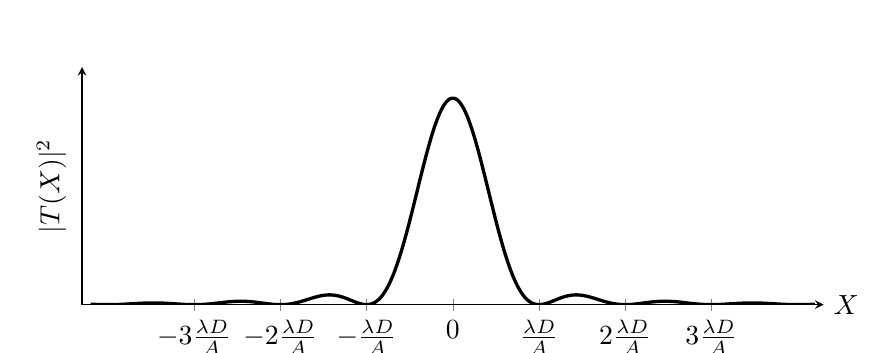
\begin{tikzpicture}
    \begin{axis}[
      width=11cm, height=4.6cm,
      xlabel={$X$}, ylabel={$|T(X)|^2$},
      axis lines=left,
      xmin=-4.3, xmax=4.3, ymin=0, ymax=1.15,
      xtick={-3,-2,-1,0,1,2,3},
      xticklabels={$-3\frac{\lambda D}{A}$,$-2\frac{\lambda D}{A}$,
                   $-\frac{\lambda D}{A}$,$0$,$\frac{\lambda D}{A}$,
                   $2\frac{\lambda D}{A}$,$3\frac{\lambda D}{A}$},
      ytick=\empty,
      every axis x label/.style={at={(current axis.right of origin)},anchor=west},
      ]
      \addplot[very thick,domain=-4.2:4.2,samples=400] {(sin(deg(pi*x))/(pi*x))^2};
    \end{axis}
  \end{tikzpicture}
\end{figure}

\begin{remark}
  Passing from the espace des positions to the espace des directions is not a
  trick reserved for diffraction. Guides à cristaux photoniques : réflexion par
  bande photonique interdite, described in $\v{k}$ space. Mécanique quantique :
  bandes d'énergie exprimées dans le domaine des $\v{k}$ ! Cristal = milliards
  d'atomes : vu le nombre d'atomes, loin des bords, pas de différence entre le
  $n$-ième et le $(n{+}1)$-ième --- l'espace des positions est peu pertinent.
  Connaître les directions de périodicité est plus pertinent.
\end{remark}

\subsubsection{Expression de la transmittance}
Nous avons raisonné jusqu'à présent en supposant que la phase accumulée est la
même en tout point de l'écran diffractant. On peut généraliser en supposant
qu'il y a à la fois des variations d'amplitude et de phase ! Ces variations
peuvent être produites en plaçant dans le plan de l'écran une lame de verre dont
l'absorption et l'épaisseur sont variables :
\begin{subpart}
  \item les variations d'absorption produisent des variations d'amplitude
    $t_D(x,y)$ ;
  \item les variations d'épaisseur ou d'indice de réfraction produisent des
    variations de phase $\phi_D(x,y)$.
\end{subpart}

\begin{definition}[Transmittance]
  D'une manière générale, la transmittance de l'objet devra être identiquement
  nulle en dehors de $D$ et devra représenter ces variations. On écrira donc :
  \[
    t(x,y) = t_D(x,y)\, e^{-i\phi_D(x,y)} .
  \]
\end{definition}

\subsubsection{Expression du champ en sortie de l'écran diffractant}
Dans le cas général, on a vu qu'à l'infini, la répartition du champ correspond à
la TF du produit du champ incident par la transmittance :
\begin{equation*}
  T(u,v) \propto TF\!\left[E_{\text{incident}}(x,y)\, t(x,y)\right]
         \propto TF\!\left[A_0(x,y)\, e^{-i\phi_0(x,y)}\,
                           t_D(x,y)\, e^{-i\phi_D(x,y)}\right],
\end{equation*}
avec $z = 0$ au niveau de l'écran diffractant. Dans le cas d'une onde plane se
propageant parallèlement à l'axe $Oz$, la répartition transverse du champ est
constante. On peut donc écrire le champ incident comme
$E_{\text{incident}}(x,y,z,t) = E_0$ en $z=0$, $t=0$, sans perte de généralité
puisque la TF ne dépend ni de $z$, ni de $t$ !

\begin{corollary}
  \[
    T(u,v) \propto E_0\, TF\!\left[t_D(x,y)\, e^{-i\phi_D(x,y)}\right].
  \]
  Dans le cas d'un écran diffractant éclairé par une onde plane parallèle à
  l'axe $Oz$, l'amplitude complexe de l'onde diffractée à l'infini est
  proportionnelle à la TF de la transmittance de l'écran diffractant.
\end{corollary}

\subsubsection{Où se trouve l'infini ?}
Lorsque $L$ est suffisamment grand, on peut admettre que
\begin{equation*}
  e^{-i\pi\frac{(x^2+y^2)}{\lambda L}} \approx 1 - i\pi\frac{(x^2+y^2)}{\lambda L},
\end{equation*}
et voyons à quelle distance le terme de phase quadratique négligé est 100 fois
plus petit que $1$ (critère arbitraire). On veut :
\begin{equation*}
  \pi\frac{(x^2+y^2)}{\lambda L} < 0.01
  \qquad\Longleftrightarrow\qquad
  L > 100\pi\, \frac{(x^2+y^2)}{\lambda}.
\end{equation*}

\begin{example}
  À $\lambda = 0.6\,\mu\mathrm{m}$ :
  \begin{subpart}
    \item pour une ouverture de $100\,\mu\mathrm{m}$ de diamètre,
      $(x^2+y^2) = r^2 =
      0.25 \cdot 10^{-8}\,\mathrm{m}^2$, soit $z > 1.3\,\mathrm{m}$ ;
    \item pour une ouverture de $1\,\mathrm{cm}$ de diamètre,
      $(x^2+y^2) = r^2 =
      2.5 \cdot 10^{-5}\,\mathrm{m}^2$, soit $z > 13\,000\,\mathrm{m}$.
  \end{subpart}
  Observer de la diffraction sur des ouvertures micrométriques est finalement
  assez simple, l'infini est relativement proche ! Par contre pour un objet
  centimétrique, il est probable qu'à $13\,\mathrm{km}$, il ne reste plus
  beaucoup d'énergie pour observer le phénomène !
\end{example}

\subsection{Diffraction par une lentille}

\subsubsection{Étude intuitive \#1 : la lentille, une transformée de Fourier}
Une source ponctuelle placée au foyer objet d'une lentille génère en sortie une
onde plane déphasée. Que somme-t-on dans le plan focal image ? Des ondes
planes ! Avec $\theta_X = X/f$ et $\theta_x = x/f$,
\begin{equation*}
  T(X) \propto \sum \left[ t_1 \mathbf{1}(x)
     + t_2\, e^{-j\frac{2\pi}{\lambda} X \theta_{x2}} + \cdots \right]
     = \sum \left[ t_1 \mathbf{1}(x)
     + t_2\, e^{-j\frac{2\pi}{\lambda} X \frac{x_2}{f}} + \cdots \right],
\end{equation*}
puis on somme cette fois de façon continue des ondes planes, comme pour la
diffraction à l'infini :
\begin{equation*}
  T\!\left(\frac{X}{\lambda f}\right) = T\!\left(\frac{\theta_X}{\lambda}\right)
  = T(u) \propto \int_{-\infty}^{+\infty} t(x)\,
    e^{-j2\pi x \frac{\theta_X}{\lambda}}\, dx .
\end{equation*}
On retrouve l'expression d'une TF. Les variables duales sont d'un côté l'espace
et de l'autre une variable angulaire comme dans le cas de la diffraction à
l'infini ! $T(u)$ est à nouveau un spectre angulaire !

\subsubsection{Étude intuitive \#2 : la lentille, une transformée de Fourier}
Comme on vient de le voir, tant que l'objet diffractant est petit (inférieur à
$100\,\mu\mathrm{m}$), « l'infini » n'est pas si loin, c'est-à-dire à quelques
mètres. Par contre, pour des objets plus grands, on voit que rapidement,
« l'infini » peut se trouver très loin ! L'observation de la diffraction de
Fraunhofer se trouve donc souvent très difficile. Pour résoudre ce problème, la solution est d'utiliser
une lentille convergente. En effet, une lentille convergente éclairée par une
onde plane (dont les faisceaux se croisent à l'infini) focalise tous les rayons
dans son \textbf{plan focal image} (\textit{image focal plane}) en un point. En
d'autres termes, la lentille ramène dans son plan focal image ce qu'il se passe
à l'infini. Or, en diffraction à l'infini (Fraunhofer), les ondes sphériques
secondaires de Huygens-Fresnel issues de l'écran diffractant sont assimilables à
des ondes planes !

\begin{theorem}[La lentille, une transformée de Fourier]
  Une lentille convergente effectue une transformée de Fourier de la répartition
  du champ complexe depuis son plan focal objet vers son plan focal image. Les
  variables conjuguées sont d'une part, l'espace $(x,y)$ dans le plan focal
  objet et d'autre part, les fréquences spatiales $(u,v)$ dans le plan focal
  image $(X,Y)$, avec
  \[
    u = \frac{X}{\lambda f}, \qquad v = \frac{Y}{\lambda f},
  \]
  où $f$ est la distance focale de la lentille.
\end{theorem}

\begin{figure}[h!]
  \centering
  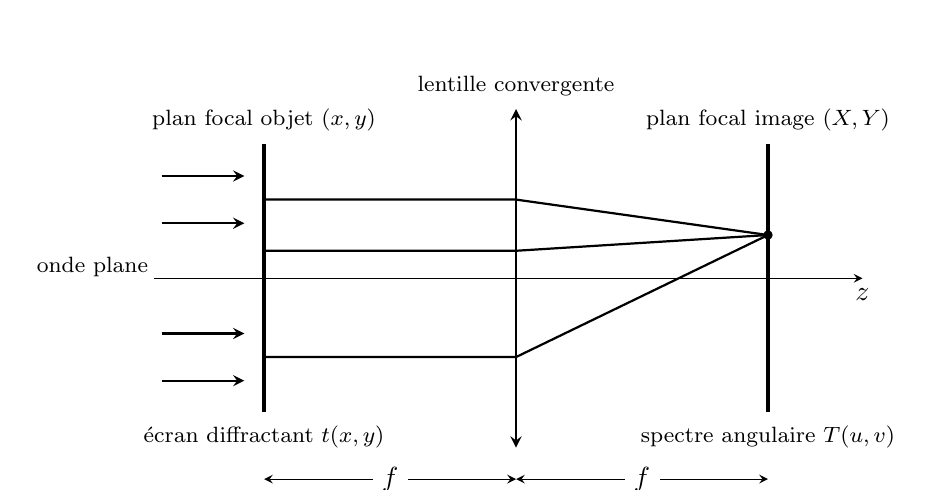
\begin{tikzpicture}[>=stealth]
    % object focal plane
    \draw[very thick] (0,-1.7) -- (0,1.7);
    \node[above] at (0,1.75) {\footnotesize plan focal objet $(x,y)$};
    \node[below] at (0,-1.75) {\footnotesize écran diffractant $t(x,y)$};
    % lens
    \draw[thick] (3.2,-1.85) -- (3.2,1.85);
    \draw[->,thick] (3.2,1.85) -- (3.2,2.15);
    \draw[->,thick] (3.2,-1.85) -- (3.2,-2.15);
    \node[above] at (3.2,2.2) {\footnotesize lentille convergente};
    % image focal plane
    \draw[very thick] (6.4,-1.7) -- (6.4,1.7);
    \node[above] at (6.4,1.75) {\footnotesize plan focal image $(X,Y)$};
    \node[below] at (6.4,-1.75) {\footnotesize spectre angulaire $T(u,v)$};
    % axis
    \draw[->] (-1.4,0) -- (7.6,0) node[below] {$z$};
    % incident plane wave
    \foreach \yy in {-1.3,-0.7,0.7,1.3}{%
      \draw[->,thick] (-1.3,\yy) -- (-0.25,\yy);}
    \node[left] at (-1.35,0.15) {\footnotesize onde plane};
    % rays through lens
    \draw[thick] (0,1.0) -- (3.2,1.0) -- (6.4,0.55);
    \draw[thick] (0,-1.0) -- (3.2,-1.0) -- (6.4,0.55);
    \draw[thick] (0,0.35) -- (3.2,0.35) -- (6.4,0.55);
    \fill (6.4,0.55) circle (1.7pt);
    % distances
    \draw[<->] (0,-2.55) -- (3.2,-2.55) node[midway,fill=white] {$f$};
    \draw[<->] (3.2,-2.55) -- (6.4,-2.55) node[midway,fill=white] {$f$};
  \end{tikzpicture}
\end{figure}

\begin{remark}
  Rigoureusement, la TF exacte est réalisée entre le plan focal \emph{objet} et
  le plan focal \emph{image}. Lorsque l'élément diffractant n'est pas dans le
  plan focal objet, on obtient la même image dans le plan focal image. En fait,
  les calculs laissent apparaître un terme de phase invisible en intensité. This
  can be checked experimentally.
\end{remark}

\subsubsection{La transformée de Fourier par une lentille : calcul explicite}
Cela peut se démontrer de manière rigoureuse en traitant la lentille comme un
masque de phase quadratique ayant un rayon de courbure fonction de la focale.
Write $(\xi,\eta)$ for the transverse coordinates in the plane of the lentille.

\begin{remark}
  The demonstration followed here is written in the \emph{opposite} sign
  convention from the rest of this chapter. The onde incidente is still
  $e^{-ikz}$, but the fonction de transmission is $e^{+i\phi}$ where the
  transmittance above is $t_D e^{-i\phi_D}$, the propagator is $e^{+ikf}$ where
  the one above is $e^{-ikL}$, and the Fresnel kernel is
  $e^{+\frac{ik}{2f}[\cdots]}$ where the one above is
  $e^{-\frac{ik}{2L}[\cdots]}$. The formula applied below is therefore the
  complex conjugate, exponent by exponent, of the expression for $U(P)$ derived
  earlier in this chapter (the prefactor is unchanged, since $1/i = -i$). The
  convention is internally coherent throughout the proof and the result is
  unaffected; this is the same non-universality of the convention already noted
  for the Fraunhofer exponent.
\end{remark}

\paragraph{Fonction de transmission.} The lentille is thin enough that the
lateral translation of the field may be neglected: a small pencil of light
enters at $(\xi,\eta)$ and leaves at $(\xi,\eta)$. If $d(\xi,\eta)$ is the
thickness of glass crossed and $n$ its index, the dephasing on crossing is
$\phi_1(\xi,\eta) = \frac{2\pi n}{\lambda} d(\xi,\eta)$. Between two planes
tangent to the lentille and separated by its maximum thickness $d_0$, the rest
of the path being air,
\begin{equation*}
  \phi(\xi,\eta) = \frac{2\pi n}{\lambda} d(\xi,\eta)
                 + \frac{2\pi}{\lambda}\left(d_0 - d(\xi,\eta)\right)
                 = \frac{2\pi}{\lambda} d_0
                 + \frac{2\pi(n-1)}{\lambda} d(\xi,\eta),
\end{equation*}
so the onde incidente is multiplied by the \textbf{fonction de transmission}
(\textit{transmission function})
\begin{equation*}
  t(\xi,\eta) = e^{i\phi(\xi,\eta)}
              = e^{2i\pi d_0/\lambda}\, e^{2i\pi(n-1)d/\lambda}.
\end{equation*}

\paragraph{L'épaisseur.} Cut the lentille in two along its thickness, with faces
of radii $R_1$ and $R_2$ ($R_2 < 0$):
\begin{equation*}
  d_1 = d_{01} - \left\{ R_1 - \sqrt{R_1^2 - \xi^2 - \eta^2}\right\},
  \qquad
  d_2 = d_{02} - \left\{ -R_2 - \sqrt{R_2^2 - \xi^2 - \eta^2}\right\},
\end{equation*}
whence
\begin{equation*}
  d(\xi,\eta) = d_1 + d_2 = d_0 - \left\{
    R_1 - \sqrt{R_1^2 - \xi^2 - \eta^2} - R_2 - \sqrt{R_2^2 - \xi^2 - \eta^2}
  \right\}.
\end{equation*}
In the paraxial approximation $\xi, \eta \ll R_1, R_2$ and
\begin{equation*}
  R_1 - \sqrt{R_1^2 - \xi^2 - \eta^2}
  = R_1 - R_1\sqrt{1 - \frac{\xi^2}{R_1^2} - \frac{\eta^2}{R_1^2}}
  \simeq \frac{1}{2R_1}\left(\xi^2 + \eta^2\right),
\end{equation*}
so that
\begin{equation*}
  d(\xi,\eta) = d_0 - \frac{1}{2}\left(\xi^2 + \eta^2\right)
                \left[\frac{1}{R_1} - \frac{1}{R_2}\right],
\end{equation*}
and the phase in $t(\xi,\eta)$ becomes
\begin{equation*}
  \phi(\xi,\eta) = \frac{2\pi n}{\lambda} d_0
    - \frac{\pi(n-1)}{\lambda}\left(\xi^2+\eta^2\right)
      \left[\frac{1}{R_1} - \frac{1}{R_2}\right].
\end{equation*}

\paragraph{La distance focale.} This forces the definition
$1/f = (n-1)\left[1/R_1 - 1/R_2\right]$ (the lensmaker's relation), with $f$
indeed the focal length, and
\begin{equation*}
  \boxed{\;
    t(\xi,\eta) = e^{2i\pi n d_0/\lambda}\,
                  e^{-i\pi(\xi^2+\eta^2)/\lambda f}
  \;}
\end{equation*}
The lentille is a pure quadratic phase mask, up to a constant phase.

\begin{example}[Consistency check]
  Let an onde plane $E_i = e^{-ikz}$ be incident on the lentille. The
  transmitted onde is
  \[
    E_t = E_i\, t(\xi,\eta)
        = e^{2i\pi n d_0/\lambda}\,
          e^{-\frac{2i\pi}{\lambda}\left(z + \frac{\xi^2+\eta^2}{2f}\right)},
  \]
  which is an onde sphérique of radius $f$. The lentille transforms an incident
  onde plane into an onde sphérique converging at its image focus --- exactly
  the result used in optique géométrique.
\end{example}

\begin{proof}[Objet contre la lentille, puis objet dans le plan focal objet]
  Consider first a plane object --- a photographic transparency --- placed
  against the lentille, emitting a field $U_i(\xi,\eta)$. Take the pupil function
  equal to $1$, so as not to add the diffraction by the finite aperture of the
  lentille. The field transmitted by the lentille is
  \[
    U_t(\xi,\eta) = U_i(\xi,\eta)\, e^{2i\pi n d_0/\lambda}\,
                    e^{-i\pi(\xi^2+\eta^2)/\lambda f}.
  \]
  Apply the diffraction formula of the approximation de Fresnel over the
  distance $f$ to reach the focal plane:
  \[
    U(x,y) = -\frac{i}{\lambda}\frac{e^{ikf}}{f}
      \iint_{-\infty}^{+\infty}
      e^{\frac{ik}{2f}\left[(x-\xi)^2 + (y-\eta)^2\right]}\,
      U_t(\xi,\eta)\, d\xi\, d\eta .
  \]
  Substituting $U_t$ and using $k/2f = \pi/\lambda f$, the quadratic phase of the
  lentille cancels the $\xi^2 + \eta^2$ produced by expanding the square,
  leaving
  \[
    U(x,y) = -\frac{i}{\lambda}\frac{e^{ikf}}{f}\, e^{2i\pi n d_0/\lambda}\,
      e^{i\pi(x^2+y^2)/\lambda f}
      \iint_{-\infty}^{+\infty} U_i(\xi,\eta)\,
      e^{-\frac{2i\pi}{\lambda f}\left(x\xi + y\eta\right)}\, d\xi\, d\eta .
  \]
  Posing the fréquences spatiales
  \[
    f_x = \frac{\alpha}{\lambda} = \frac{x}{\lambda f},
    \qquad
    f_y = \frac{\beta}{\lambda} = \frac{y}{\lambda f},
  \]
  the integral is the spatial transformée de Fourier $\tilde{U}_i(f_x,f_y)$ of
  $U_i(\xi,\eta)$, and the prefactor $e^{i\pi(x^2+y^2)/\lambda f}$ can be pulled
  out as $e^{i\pi\lambda f (f_x^2 + f_y^2)}$:
  \[
    U(x,y) = \text{Cste}\cdot L(x,y)\cdot \tilde{U}_i(f_x,f_y),
    \qquad
    L(x,y) = e^{i\pi(x^2+y^2)/\lambda f}.
  \]
  The image of $U_i$ in the focal plane is thus its transformée de Fourier
  modified by the \textbf{fonction « loupe »} (\textit{magnifier function})
  $L(x,y)$.\\

  Now move the object out of contact with the lentille and into the \emph{plan
  focal objet}. Let it carry a field $U_0(x_1,y_1)$ with spectre angulaire
  \[
    \tilde{U}_0(f_x,f_y) = \iint_{-\infty}^{+\infty} U_0(x_1,y_1)\,
      e^{-2i\pi\left(f_x x_1 + f_y y_1\right)}\, dx_1\, dy_1 .
  \]
  Propagating over the distance $f$ up to the entrance plane of the lentille, the
  spectre angulaire arriving on the lentille is
  \[
    \tilde{U}_i(f_x,f_y) = \tilde{U}_0(f_x,f_y)\, e^{2i\pi f/\lambda}\,
      e^{-i\pi\lambda f\left(f_x^2 + f_y^2\right)} .
  \]
  Inserting this into the previous relation, the two quadratic phases
  $e^{+i\pi\lambda f(f_x^2+f_y^2)}$ and $e^{-i\pi\lambda f(f_x^2+f_y^2)}$ cancel
  exactly:
  \[
    U(x,y) = -\frac{i}{\lambda}\frac{e^{ikf}}{f}\, e^{2i\pi n d_0/\lambda}\,
       e^{i\pi\lambda f (f_x^2+f_y^2)}\, \tilde{U}_0(f_x,f_y)\,
       e^{2i\pi f/\lambda}\, e^{-i\pi\lambda f(f_x^2+f_y^2)}
  \]
  \[
    \boxed{\;
      U(x,y) = -\frac{i}{\lambda f}\, e^{2ikf}\, e^{2i\pi n d_0/\lambda}\,
               \tilde{U}_0(f_x,f_y)
    \;}
  \]
  The function $L(x,y)$ has disappeared and the image observed in the plan
  focal image is proportional to the transformée de Fourier of the object. \qed
\end{proof}

\begin{conclusion}
  The quadratic phase mask of the lentille always cancels the quadratic phase of
  the Fresnel kernel --- that is what makes the focal-plane field a transformée
  de Fourier at all, object against the lentille included, and it owes nothing
  to where the object sits. What the plan focal objet buys is the
  \emph{second} cancellation: propagation over $f$ from that plane imprints
  $e^{-i\pi\lambda f(f_x^2+f_y^2)}$, exactly the inverse of the residual
  fonction « loupe » $L(x,y)$, so only then is the focal-plane field
  proportional to the bare transform. Placed against the lentille, the object
  still gives its transformée de Fourier, but multiplied by $L(x,y)$ --- a pure
  phase, hence invisible in intensity, which is why the two configurations look
  the same on a screen.
\end{conclusion}

\subsubsection{Méthode de travail : diffraction par une lentille convergente}
Pour résoudre un problème de diffraction par une lentille convergente, la
méthode est toujours la même.
\begin{enumerate}
  \item Dans le plan focal objet, en coordonnées $(x,y)$ : exprimer le champ
    incident ; exprimer la transmittance de l'objet diffractant ; en déduire
    l'expression du champ en sortie de l'écran diffractant.
  \item Dans le plan focal image : calculer l'expression du spectre angulaire
    $T(u,v)$ diffracté dans le plan focal image par transformée de Fourier du
    champ précédent (coordonnées $(u,v)$).
  \item En déduire l'expression du champ diffracté dans le plan focal image, en
    coordonnées spatiales $(X,Y)$ en utilisant le changement de variable
    $u = X/\lambda f$, $v = Y/\lambda f$.
  \item En déduire l'intensité diffractée dans le plan focal image (coordonnées
    $(u,v)$ ou $(X,Y)$).
\end{enumerate}

\subsection{Propriétés générales reliant l'écran diffractant et la figure de diffraction}
Le but de ce paragraphe est de reprendre les propriétés de la TF énoncées dans
le domaine Temps/Fréquence au domaine de la diffraction dans le domaine
Espace/Fréquence spatiale --- with the sign conventions of this chapter.

\subsubsection{TF d'une ouverture carrée}
On peut décomposer la transmittance d'une ouverture carrée de côté $A$ en deux
fonctions à variable séparable :
\begin{equation*}
  t(x,y) = \bm{\pi}_A(x)\, \bm{\pi}_A(y),
\end{equation*}
et le spectre angulaire est la TF de la transmittance puisque l'écran est
éclairé par une onde plane :
\begin{equation*}
  T(u,v) = T\!\left(\frac{\theta_X}{\lambda}\right)
           T\!\left(\frac{\theta_Y}{\lambda}\right)
         \propto \frac{\sin \pi u A}{\pi u A}\,\frac{\sin \pi v A}{\pi v A}.
\end{equation*}
Sur l'écran, on observe l'intensité du signal après le changement de variables,
soit une image de la forme
\begin{equation*}
  |T(X,Y)|^2 \propto
    \left|\frac{\sin \pi \frac{X}{\lambda f}A}{\pi \frac{X}{\lambda f}A}\right|^2
    \left|\frac{\sin \pi \frac{Y}{\lambda f}A}{\pi \frac{Y}{\lambda f}A}\right|^2 ,
\end{equation*}
--- a cross-shaped grid of spots whose central lobe has half-width
$\lambda f / A$.

\subsubsection{TF d'une fente infiniment fine}
On éclaire cette fois une fente infiniment fine et infiniment haute, centrée en
$x=0$. Sa transmittance peut s'exprimer comme $t(x,y) = \delta(x)\mathbf{1}(y)$.
Si on calcule le spectre angulaire diffracté dans le plan focal image, on trouve
cette fois un trait \emph{horizontal} infiniment fin :
\begin{equation*}
  T(u,v) = T\!\left(\frac{\theta_X}{\lambda}\right)
           T\!\left(\frac{\theta_Y}{\lambda}\right)
         \propto \mathbf{1}(u)\,\delta(v),
  \qquad
  |T(X,Y)|^2 \propto |\mathbf{1}(X)|^2 |\delta(Y)|^2 .
\end{equation*}
The pattern is rotated by $90^\circ$ with respect to the object. Ce résultat est
compatible avec la propriété de changement d'échelle below: infinitely narrow
in $x$ gives infinitely wide in $u$, and infinitely wide in $y$ gives
infinitely narrow in $v$. For comparison, a point source centred at the origin
is $t(x,y) = \delta(x)\delta(y)$.

\subsubsection{Dilatation et contraction de l'ouverture du diaphragme}
Si on dilate ou contracte les coordonnées dans l'espace direct, ce qui revient à
multiplier par $a$ et $b$ les dimensions de l'ouverture, on observe inversement
une contraction ou dilatation de l'espace spectral et un changement de
l'amplitude du spectre :
\begin{equation*}
  TF\!\left[t(ax,by)\right] = \frac{1}{|a|}\frac{1}{|b|}\,
    T\!\left(\frac{u}{a}, \frac{v}{b}\right).
\end{equation*}
Plus l'ouverture est petite, plus l'image au foyer image de la lentille est
étalée. The factor $1/|a||b|$ is an energy-conservation factor, as the théorème
de Parseval-Plancherel shows.

\subsubsection{Translation dans son plan du diaphragme limitant la surface d'onde}
Une translation de la fonction $t(x,y)$ dans le plan focal objet se traduit par
la multiplication de l'amplitude de la figure de diffraction par un terme de
phase :
\begin{equation*}
  TF\!\left[t(x-a, y-b)\right] = e^{+2i\pi u a}\, e^{+2i\pi v b}\, T(u,v).
\end{equation*}
Or, en intensité, un terme de phase est invisible puisque son module vaut $1$ !
Donc, \emph{cette translation ne modifiera pas l'image diffractée au plan focal
image}. Réciproquement, un déphasage de l'écran de diffraction provoque un
déplacement de la figure de diffraction. Note that the exponent here carries
$e^{+2i\pi ua}$ where the chapter-2 translation property reads
$TF[f(t-\tau)] = e^{-2i\pi\nu\tau}F[\nu]$: the same inverse-versus-direct
convention swap already noted for the Fraunhofer exponent, and invisible in
intensity either way.

\subsubsection{Succession de transformées de Fourier}
\begin{prop}
  \[
    TF^{-1}\!\left[TF[f(x)]\right] = f(x),
    \qquad
    TF\!\left[TF[f(x)]\right] = f(-x)
    \quad\text{or}\quad
    TF^{-1}\!\left[TF^{-1}[f(x)]\right] = f(-x).
  \]
\end{prop}
Lorsque l'on place une lentille derrière une autre, les deux effectuent la
\emph{même} opération, so two lentilles give $f(-x)$. Conformément à l'optique
géométrique, l'image après deux lentilles est identique à l'originale mais
retournée. Pour simplifier les calculs, on s'affranchira souvent du retournement
de l'image en orientant à l'envers l'axe dans le plan image.

\subsubsection{Distribution peigne de Dirac}
\begin{definition}[Peigne de Dirac]
  Le peigne de Dirac de raison $a$ et son spectre sont :
  \[
    \omega_a(x) = \sum_{n=-\infty}^{+\infty} \delta(x - na),
    \qquad
    TF\!\left[\omega_a(x)\right] = \frac{1}{a}\,\omega_{1/a}(u)
      = \frac{1}{a}\sum_{n=-\infty}^{+\infty} \delta\!\left(u - \frac{n}{a}\right).
  \]
\end{definition}
A comb of pitch $a$ transforms into a comb of pitch $1/a$ and poids $1/a$ --- the
changement d'échelle property again.

\subsection{Convolution et multiplication}

\begin{definition}[Produit de convolution (\textit{convolution product})]
  \[
    h(x) = (f * f')(x) = \int_{-\infty}^{+\infty} f(x')\, f'(x-x')\, dx' .
  \]
\end{definition}

Le produit de convolution est essentiel en physique car il apparaît dès que l'on
effectue une \emph{mesure} mais il peut être dur à calculer.

\begin{theorem}[Théorème de convolution (\textit{convolution theorem})]
  La TF d'un produit de convolution $(*)$ de deux fonctions est égale au produit
  simple $(\times)$ des TF et réciproquement :
  \[
    (f * g)(x)
    \quad\stackrel{TF}{\longleftrightarrow}\quad
    \hat{F}(u) \times \hat{G}(u).
  \]
\end{theorem}

On voit qu'un calcul de convolution qui peut être très complexe peut se
transformer en un produit bien plus simple en passant par transformée de Fourier
dans le domaine dual.

\begin{remark}
  Attention au cas de la TF à deux dimensions : convoluer deux fonctions de
  variables \emph{différentes} n'a aucun sens physique, c'est donc interdit. À
  deux dimensions, dans le cas de fonctions à variables séparables, une
  multiplication reste donc une multiplication ! On écrira :
  \[
    f(x) \times g(y)
    \quad\stackrel{TF}{\longleftrightarrow}\quad
    \hat{F}(u) \times \hat{G}(v),
  \]
  which is immediate from
  $TF[f(x)g(y)] = \iint f(x)g(y) e^{-2j\pi(ux+vy)}dx\,dy
   = \int f(x)e^{-2j\pi ux}dx \int g(y)e^{-2j\pi vy}dy$.
\end{remark}

\begin{prop}[Quelques propriétés du produit de convolution]
  \begin{subpart}
    \item commutatif : $(f*g)(x) = (g*f)(x)$ ;
    \item associatif : $\left(f*(g*h)\right)(x) = \left((f*g)*h\right)(x)$ ;
    \item distributif : $\left([a\cdot f + b\cdot g] * h\right)(x)
      = a\cdot(f*h)(x) + b\cdot(g*h)(x)$.
  \end{subpart}
\end{prop}

\subsubsection{Convolution d'une fonction avec un Dirac ou un peigne de Dirac}
D'après ce qui précède (théorème de convolution), on peut écrire :
\begin{equation*}
  TF\!\left[(f*\delta)(x)\right] = TF[f(x)]\, TF[\delta(x)] = TF[f(x)],
  \qquad\text{hence}\qquad
  (f*\delta)(x) = \int f(x')\delta(x-x')dx' = f(x).
\end{equation*}
\emph{Le Dirac est l'élément neutre de la convolution !} Plus intéressant encore,
la convolution d'une fonction avec un Dirac décentré donne, en effectuant un
changement de variable adéquat :
\begin{equation*}
  \boxed{\; f(x) * \delta(x-a) = f(x-a) \;}
\end{equation*}
La convolution d'une fonction avec un Dirac décentré redonne la même fonction
mais centrée à la position du Dirac. Cette opération permet donc de
\textbf{translater} une fonction. On constate que, bien que le Dirac n'ait pas
de réalité physique, sa convolution avec une fonction donne une fonction, le
résultat a donc une réalité physique.

La convolution ainsi que la TF étant distributives, on obtient naturellement :
\begin{equation*}
  f(x) * \omega_a(x) = f(x) * \sum_{n=-\infty}^{+\infty}\delta(x - na)
                     = \sum_{n=-\infty}^{+\infty} f(x - na) .
\end{equation*}
La convolution d'une fonction avec une somme de Diracs permet donc de
\textbf{périodiser} une fonction. C'est comme cela que nous représenterons les
fonctions périodiques, avec $f(x)$ qui représentera le motif élémentaire. Cela
facilitera grandement les calculs.

\subsubsection{Multiplication d'une fonction avec un Dirac}
\begin{equation*}
  \boxed{\; f(x) \times \delta(x-a) = f(a)\,\delta(x-a) \;}
\end{equation*}
L'intérêt de cette propriété est de simplifier les calculs en transformant une
fonction en une constante, la valeur de la fonction à la position du Dirac.
Cette constante modifie « le poids » du Dirac. Attention, il est indispensable
de ne pas oublier le Dirac sans quoi le résultat est complètement faux !

\begin{conclusion}[Convolution ou multiplication ?]
  Pas de hasard ! On utilisera la \textbf{multiplication} pour modifier les
  amplitudes d'une fonction ; on utilisera la \textbf{convolution avec un Dirac}
  pour translater une fonction.
\end{conclusion}

\begin{example}[The monochromator]
  A monochromator disperses the spectrum in space and scans it with a moving slit
  in front of a detector. The measured signal is the real spectrum convolved with
  the sliding window, which is a porte:
  \[
    S_{\text{mesuré}}(\lambda) = \int_{-\infty}^{+\infty}
      S_{\text{réel}}(x')\, \underbrace{\bm{\pi}(\lambda - x')}
      _{\text{fenêtre glissante} \,=\, \text{porte}}\, dx' .
  \]
  When the window is narrow, $\bm{\pi}_\varepsilon \to \delta$ and the measured
  spectrum is the real one; when it is broad, the fine structure is smoothed away.
  Every instrument convolves what it measures by its own \textit{fonction
  d'appareil}.
\end{example}

\begin{example}[Listening to a sound]
  In the frequency domain, the spectrum $S(\nu)$ of a sound is \emph{multiplied}
  by the filtre passe-bande of the ear, of bande passante $BP$. In the time
  domain the same operation is a convolution of $s(t) = TF[S(\nu)]$ by the instrument
  function $TF[\text{filtre de l'oreille}]$, whose width is the integration time
  $\Delta\tau \propto 1/BP$ of the detector. A sound too high in pitch oscillates
  faster than $\Delta\tau$, is averaged out, and is not heard.
\end{example}

\subsection{Lien entre variations d'intensité dans une image et fréquences spatiales}
Une fréquence spatiale peut être vue comme un angle qui dépend de la longueur
d'onde. En d'autres termes, dans le plan focal image d'une lentille, plus les
fréquences spatiales sont élevées, plus l'énergie se retrouve répartie loin de
l'axe optique. Plus les fréquences spatiales sont basses, plus l'énergie se
retrouve proche de l'axe optique.

\subsubsection{Signification de $T(0,0)$}
Si on reprend l'expression de la TF en $u = v = 0$, on obtient :
\begin{equation*}
  T(u,v)\big|_{u=v=0} \propto \iint_{-\infty}^{+\infty}
    E_{\text{incident}}(x,y)\, t(x,y)\, e^{-2i\pi(0x+0y)}\, dx\, dy
  \propto \iint_{-\infty}^{+\infty} E_{\text{incident}}(x,y)\, t(x,y)\, dx\, dy ,
\end{equation*}
c'est bien la \emph{moyenne} de l'onde dans le plan focal objet --- the centre
of the figure de diffraction carries the continuous background of the image.

\subsubsection{Signification de $T(u,v)$ pour $u,v$ différents de 0}
Prenons un \textbf{réseau sinusoïdal} (\textit{sinusoidal grating}) de pas $a$,
de dimension infinie dans les deux directions :
\begin{equation*}
  t_{\substack{\text{réseau}\\ \text{infini}}}(x,y)
    = \left(\frac{1}{2} + \cos\left(\frac{2\pi x}{a}\right)\right)\mathbf{1}(y),
\end{equation*}
avec $\mathbf{1}(y)$ la fonction qui vaut $1$ quel que soit $y$. Dans le plan
focal image de la lentille, on observe la TF de l'écran diffractant :
\begin{equation*}
  T_{\substack{\text{réseau}\\ \text{infini}}}(u,v)
    = \frac{1}{2}\left(\delta(u)
      + \delta\!\left(u + \frac{1}{a}\right)
      + \delta\!\left(u - \frac{1}{a}\right)\right)\delta(v).
\end{equation*}

\begin{remark}
  La fonction $\mathbf{1}(y)$ semble ne servir à rien. Il est vrai que ne pas
  l'écrire n'est pas faux. Par contre, l'omettre, c'est très souvent oublier
  d'en faire la TF, ce qui modifie notablement le résultat car
  $TF[\mathbf{1}(y)] = \delta(v)$.
\end{remark}

On observe donc deux taches au côté de la tache centrale.
\begin{subpart}
  \item La tache centrale $\delta(u)$ porte l'information sur le fond continu
    --- la valeur moyenne --- de l'écran diffractant.
  \item Les deux taches adjacentes $\delta(u \pm 1/a)$ sont la signature
    spectrale de la variation d'amplitude sinusoïdale de l'écran de diffraction.
  \item L'extension suivant $Y$ est nulle, $\delta(v)$, puisqu'elle était
    infinie, $\mathbf{1}(y)$, dans l'écran diffractant.
\end{subpart}

On peut tronquer mathématiquement le réseau de dimension infinie en le
multipliant par une porte de largeur adéquate $A$ :
\begin{equation*}
  t_{\substack{\text{réseau}\\ \text{tronqué}}}(x,y)
    = \bm{\pi}\!\left(\frac{x}{A}\right) \times
      t_{\substack{\text{réseau}\\ \text{infini}}}(x,y),
\end{equation*}
and by the théorème de convolution the multiplication in direct space becomes a
convolution in the spectral space:
\begin{align*}
  T_{\substack{\text{réseau}\\ \text{tronqué}}}(u,v)
  &= TF\!\left[\bm{\pi}\!\left(\frac{x}{A}\right)\right] *
     T_{\substack{\text{réseau}\\ \text{infini}}}(u,v) \\
  &= \frac{1}{2} A \frac{\sin \pi u A}{\pi u A} *
     \left(\delta(u) + \delta\!\left(u+\frac{1}{a}\right)
     + \delta\!\left(u-\frac{1}{a}\right)\right)\delta(v) \\
  &\propto \left(\frac{\sin \pi u A}{\pi u A}
     + \frac{\sin \pi \left(u+\frac{1}{a}\right)A}{\pi\left(u+\frac{1}{a}\right)A}
     + \frac{\sin \pi \left(u-\frac{1}{a}\right)A}{\pi\left(u-\frac{1}{a}\right)A}
     \right)\delta(v).
\end{align*}
La figure de diffraction est la même que pour le réseau infini mais les pics sont
remplacés par des taches de diffraction (ici des sinus cardinaux) car le réseau
est tronqué, de largeur $A$.

\begin{figure}[h!]
  \centering
  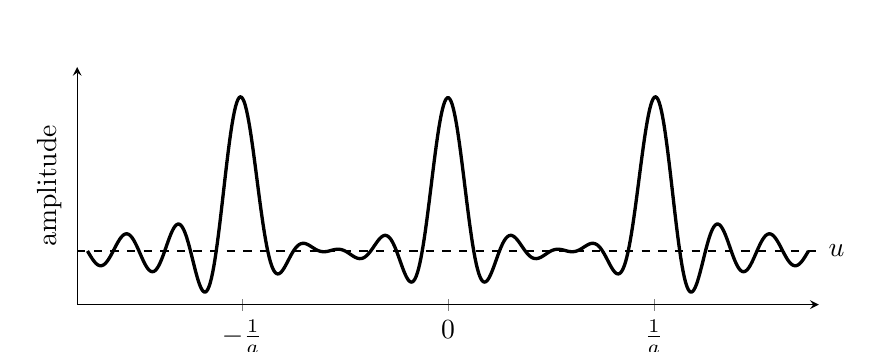
\begin{tikzpicture}
    \begin{axis}[
      width=11cm, height=4.6cm,
      xlabel={$u$}, ylabel={amplitude},
      axis lines=left,
      xmin=-3.6, xmax=3.6, ymin=-0.35, ymax=1.2,
      xtick={-2,0,2},
      xticklabels={$-\frac{1}{a}$,$0$,$\frac{1}{a}$},
      ytick=\empty,
      every axis x label/.style={at={(current axis.right of origin)},anchor=west},
      ]
      \addplot[very thick,domain=-3.5:3.5,samples=600]
        {sin(deg(pi*4*x))/(pi*4*x)
         + sin(deg(pi*4*(x+2)))/(pi*4*(x+2))
         + sin(deg(pi*4*(x-2)))/(pi*4*(x-2))};
      \draw[dashed] (axis cs:-3.6,0) -- (axis cs:3.6,0);
    \end{axis}
  \end{tikzpicture}
\end{figure}

La position des deux pics adjacents dépend de la période du réseau sinusoïdal.
En accord avec la propriété de contraction/dilatation :
\begin{subpart}
  \item plus la variation d'amplitude de l'écran diffractant est lente (large
    period), plus la fréquence est basse et la position des pics adjacents est
    proche de l'axe optique ($X$ et $Y$ faibles) ;
  \item plus la variation d'amplitude de l'écran diffractant est rapide (small
    period), plus la fréquence est élevée et la position du pic est éloignée de
    l'axe optique ($X$ et $Y$ élevés) ;
  \item l'information spectrale concernant le fond continu ou la valeur moyenne
    d'une image sera elle représentée au centre, $u = v = X = Y = 0$.
\end{subpart}

\begin{conclusion}
  Pour une image quelconque :
  \begin{subpart}
    \item les variations rapides --- les contours d'un objet, les détails, les
      rayures --- seront représentées sur l'écran de diffraction par de
      l'énergie lumineuse \emph{loin} de l'axe optique ;
    \item les variations lentes, les couleurs uniformes et la valeur moyenne de
      l'image seront représentées par de l'énergie lumineuse \emph{proche} de
      l'axe.
  \end{subpart}
  La notion de fréquence spatiale représente donc en quelque sorte le nombre de
  variations par unité de longueur. Pour un réseau, on parle de nombre de traits
  par millimètre. La figure de diffraction nous informe donc sur les
  périodicités présentes dans l'image !
\end{conclusion}

\subsection{Traitement des images}
Le filtrage est une notion finalement assez connue par bon nombre de personnes
pour peu qu'elles aient eu une fois dans leur vie un égaliseur de chaîne HIFI où
tout naturellement nous atténuons telle ou telle fréquence comme les aigus ou
les graves. Seul l'étourdi n'aura pas remarqué qu'il applique alors des
\textbf{filtres passe-bande} (\textit{band-pass filters}) laissant passer ou
coupant certaines bandes de fréquence. Avec une
lentille, nous pouvons isoler \emph{dans l'espace} telle ou telle fréquence
spatiale. Il est alors facile de comprendre que dans le plan focal image d'une
lentille, il est possible de « couper » certaines fréquences par un simple cache
pour obturer la lumière. Une lentille supplémentaire permet alors de repasser
dans l'espace principal et reconstituer l'image filtrée.

\begin{definition}[Montage 4f]
  Le \textbf{montage 4f} (\textit{4f setup}), dit « à double diffraction », est
  composé de deux lentilles placées sur le même axe optique, dont le foyer image
  de la première coïncide avec le foyer objet de la seconde. C'est ce que l'on
  appelle un \textbf{système afocal} (\textit{afocal system}). La diapositive
  dans le plan focal objet est éclairée par une onde plane. The common focal
  plane is the \textbf{plan de Fourier} (\textit{Fourier plane}), que l'on peut
  également appeler \textbf{plan de filtrage} (\textit{filtering plane}).
\end{definition}

\begin{figure}[h!]
  \centering
  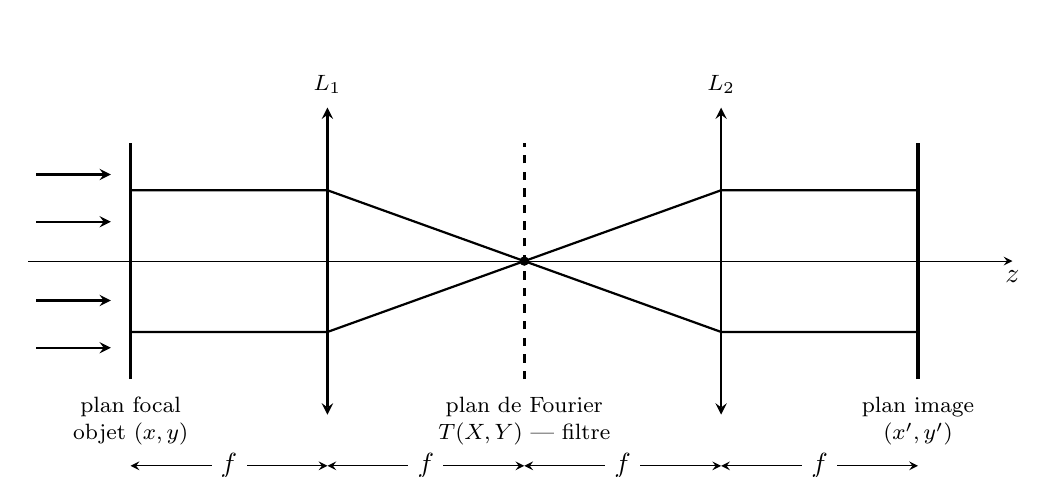
\begin{tikzpicture}[>=stealth]
    \draw[->] (-1.3,0) -- (11.2,0) node[below] {$z$};
    % object plane
    \draw[very thick] (0,-1.5) -- (0,1.5);
    \node[align=center,below] at (0,-1.6)
      {\footnotesize plan focal\\[-2pt] \footnotesize objet $(x,y)$};
    % lens 1
    \draw[thick] (2.5,-1.65) -- (2.5,1.65);
    \draw[->,thick] (2.5,1.65) -- (2.5,1.95);
    \draw[->,thick] (2.5,-1.65) -- (2.5,-1.95);
    \node[above] at (2.5,2.0) {\footnotesize $L_1$};
    % Fourier plane
    \draw[very thick,dashed] (5,-1.5) -- (5,1.5);
    \node[align=center,below] at (5,-1.6)
      {\footnotesize plan de Fourier\\[-2pt] \footnotesize $T(X,Y)$ --- filtre};
    % lens 2
    \draw[thick] (7.5,-1.65) -- (7.5,1.65);
    \draw[->,thick] (7.5,1.65) -- (7.5,1.95);
    \draw[->,thick] (7.5,-1.65) -- (7.5,-1.95);
    \node[above] at (7.5,2.0) {\footnotesize $L_2$};
    % image plane
    \draw[very thick] (10,-1.5) -- (10,1.5);
    \node[align=center,below] at (10,-1.6)
      {\footnotesize plan image\\[-2pt] \footnotesize $(x',y')$};
    % rays
    \draw[thick] (0,0.9) -- (2.5,0.9) -- (5,0.0) -- (7.5,-0.9) -- (10,-0.9);
    \draw[thick] (0,-0.9) -- (2.5,-0.9) -- (5,0.0) -- (7.5,0.9) -- (10,0.9);
    \fill (5,0) circle (1.7pt);
    % plane wave
    \foreach \yy in {-1.1,-0.5,0.5,1.1}{%
      \draw[->,thick] (-1.2,\yy) -- (-0.25,\yy);}
    % distances
    \foreach \xa/\xb in {0/2.5, 2.5/5, 5/7.5, 7.5/10}{%
      \draw[<->] (\xa,-2.6) -- (\xb,-2.6) node[midway,fill=white] {$f$};}
  \end{tikzpicture}
\end{figure}

Conformément à l'optique géométrique, sans filtrage, on retrouve l'image
identique mais inversée. C'est aussi conforme à l'optique de Fourier puisqu'après
deux TF successives :
\begin{equation*}
  TF\!\left[TF[f(x,y)]\right] = f(-x,-y).
\end{equation*}

Dans le plan de Fourier, on peut alors insérer différents masques ou filtres.
\begin{subpart}
  \item Le \textbf{filtre passe-bas} (\textit{low-pass filter}) --- une ouverture
    circulaire --- coupe les hautes fréquences. On l'a vu, ces fréquences portent
    l'information sur les détails d'une image, les variations rapides
    d'intensité. L'image filtrée se retrouvera donc \emph{floutée}.
  \item Le \textbf{filtre passe-haut} (\textit{high-pass filter}) --- une
    pastille absorbante (on the axis) --- fait l'inverse du passe-bas. Il coupe
    le fond continu d'une image et toutes les variations lentes d'intensité. Il
    ne restera donc dans l'image filtrée que les \emph{contours} des formes.
  \item Between the two sits the filtre passe-bande, an annulus.
\end{subpart}

\begin{remark}
  Two further applications: le \textit{détramage} de photo --- removing the
  printing screen of a photograph, whose regular raster shows up as isolated
  spots in the plan de Fourier that can simply be blocked --- and l'extraction
  des variations de phase invisibles à l'œil nu, a phase object being invisible
  in intensity until its spectrum is filtered.
\end{remark}

\begin{conclusion}
  The whole chapter reduces to one operation and one change of variables. At
  infinity --- or, equivalently, in the plan focal image of a lentille
  convergente --- the diffracted amplitude complexe is the transformée de
  Fourier of the field leaving the diffracting screen,
  \[
    T(u,v) \propto TF\!\left[E_{\text{incident}}(x,y)\, t(x,y)\right],
    \qquad
    u = \frac{X}{\lambda f} = \frac{\theta_X}{\lambda},
    \qquad
    v = \frac{Y}{\lambda f} = \frac{\theta_Y}{\lambda}.
  \]
  Everything else --- the sinc of a slit, the inverse scaling of the pattern with
  the aperture, the invisibility of a translation, the periodisation by a
  peigne de Dirac, low-pass and high-pass filtering --- is a property of that
  transform read in optical language.
\end{conclusion}

\section{La fibre optique}
Les communications optiques existaient déjà du temps des amérindiens avec
l'utilisation des signaux de fumée ! En 1794, le télégraphe optique de Chappe
fait son apparition. Les sémaphores étaient relativement espacés (10 à 30\,km)
et permettaient de transmettre des messages dans toute la France en quelques
heures (en 1844, il existe 5000\,km de lignes Chappe avec 534 stations
permanentes en France ; Paris--Lille : 9 minutes !). Le développement de
l'électricité fait disparaître l'optique des télécommunications avec la mise au
point en 1855 du télégraphe électrique qui permet de communiquer par
l'intermédiaire de fils métalliques, de jour comme de nuit et quelles que soient
les conditions climatiques. L'optique réapparaît vers les années 60 avec
l'apparition du laser (1960). Cependant, un faisceau lumineux qui se propage en
espace libre subit bon nombre de modifications et ce pour diverses raisons :
variation de l'indice de réfraction du chemin traversé par la lumière modifiant
perpétuellement le chemin optique vu par la lumière (variation des conditions
climatiques influant sur l'indice) ; variation de l'atténuation du milieu en
fonction des conditions atmosphériques ; diffraction d'un faisceau lumineux dont
le diamètre transverse $D$ n'est pas infini. Il subit une divergence naturelle
de l'ordre de $\theta = 10^{-4}$\,radian pour un faisceau de $D = 5$\,mm de
diamètre et une longueur d'onde de l'ordre de $\lambda \approx 0.5\,\mu$m. Il en
résulte, après une propagation sur une distance $L$, un élargissement
$\Delta D \approx L\theta$. Par exemple, pour $L = 1$\,km, l'élargissement du
faisceau est de 10\,cm. Il y a donc dispersion de l'énergie par diffraction !

Tout ceci met donc rapidement en évidence la nécessité d'une propagation guidée.
La fibre optique pour la propagation longue distance est mise au point en 1966.
La longueur totale du réseau français dépasse les quelques dizaines de millions
de kilomètres quand le réseau japonais, le plus long du monde, atteignait déjà
en 2010 plus de 110 millions de kilomètres. Débits actuels : 100\,Gb/s par
longueur d'onde installée (500\,Gb/s par longueur d'onde en laboratoire) ;
jusqu'à 88 canaux (one channel per longueur d'onde), soit quelques dizaines de Tb/s sur une fibre optique !\\

This chapter guides the light three times over, the first time by réflexion
totale interne. Après avoir présenté le guidage de la lumière dans un guide
d'onde par l'intermédiaire de l'optique géométrique, nous essayerons de
comprendre, à l'aide de l'optique ondulatoire, pourquoi certaines trajectoires
sont permises alors que d'autres ne le sont pas. Cela permettra d'aborder la
notion de mode transverse, de guide monomode ou multimode, etc. Enfin, nous
montrerons qu'il existe des outils puissants, à partir des équations de
Maxwell, qui permettent de décrire parfaitement la répartition transverse
d'énergie dans un guide aussi bien planaire qu'à symétrie de révolution.

\subsection{Notion de guide d'onde}

\begin{definition}[Guide d'onde optique]
  Un \textbf{guide d'onde} (\textit{waveguide}) optique est une structure
  diélectrique, uniforme le long d'un axe, capable de transporter de l'énergie
  électromagnétique à des longueurs d'onde situées dans les parties infrarouge
  et visible du spectre sur des distances grandes devant la longueur d'onde.
\end{definition}

Un diélectrique est un matériau qui ne possède pas de charges électriques
susceptibles de se déplacer de façon macroscopique. Ainsi, ce milieu ne conduit
pas le courant, il est isolant.\\

Dans la pratique, un guide d'onde dans le domaine optique du spectre est
constitué d'une région diélectrique planaire ou linéaire appelée
\textbf{cœur} (\textit{core}). Cette zone est entourée par un ou plusieurs
milieux diélectriques dont les indices de réfraction sont \emph{inférieurs} à
celui du cœur afin d'assurer le confinement de l'onde. Cette zone extérieure au
cœur est appelée la \textbf{gaine} (\textit{cladding}) du guide. Le cœur de
tous ces guides est l'endroit où l'énergie se propage.\\

Three geometries matter. Le guide le plus simple est le \textbf{guide d'onde
plan à saut d'indice} (\textit{plane step-index guide}) dont la dimension
suivant $y$ est infinie. Le terme « \textbf{saut d'indice} »
(\textit{step index}) signifie que l'indice est constant dans chaque domaine.
La lumière est guidée suivant l'axe $z$. Le guide rectangulaire ou
\textbf{guide à ruban} (\textit{ribbon guide}) se rencontre dans les lasers à
semi-conducteurs produits à des milliards d'exemplaires. Très compliqué, ce
guide ne sera pas étudié ici. Enfin, la fibre est un guide à symétrie de
révolution. Son étude se rapproche de celle du guide plan mais s'avère plus
complexe.

\begin{remark}
  Les méthodes numériques utilisées pour résoudre le problème de la
  propagation dans un guide diélectrique sont souvent compliquées. Nous nous
  contenterons d'analyser le guide planaire à saut d'indice. Bien que son étude
  revêt clairement un aspect idéal (dimension infinie suivant $y$), il permet
  de comprendre la plupart des mécanismes de guidage de la lumière et les
  problématiques liées au confinement de cette dernière. C'est ce guide que
  nous utiliserons lors des deux prochaines parties : approche géométrique et
  approche ondulatoire.
\end{remark}

\paragraph{Dimension typique d'une fibre} Les caractéristiques typiques d'une
fibre optique sont
\[
  n_{\text{verre}} \approx 1.44\text{--}1.46, \qquad
  \Delta n = n_{\text{cœur}} - n_{\text{gaine}} = 10^{-3}\ \text{to}\ 2\times 10^{-2},
  \qquad D_{\text{cœur}} = 2a = 5\ \text{to}\ 50\,\mu\mathrm{m}.
\]
La fibre la plus utilisée dans le domaine des télécommunications optiques
haut-débit est la fibre dite monomode standard SMF28 (\textit{Single Mode
Fiber}). Ses diamètres typiques sont $D_{\text{cœur}} =
9\,\mu$m et $D_{\text{gaine}} = 125\,\mu$m; the gaine is itself protected by a
polymer coating taking the outer diameter to
$250\,\mu$m. Cette enveloppe protectrice supplémentaire assure une protection à
la fois mécanique et surtout optique vis à vis de la lumière extérieure mais ne
participe pas au guidage. Le diélectrique utilisé est dans la plupart des cas
de la silice dopée par du bore, qui facilite la fusion du verre, empêche la
dévitrification et améliore la résistance à l'eau, et par du germanium
($n_{\text{Ge}} \approx 4.2$ à $1550$\,nm et $300$\,K), qui permet suivant sa
concentration d'augmenter l'indice du verre. D'autres ingrédients sont
également utilisés. Cette cuisine relève souvent du secret industriel dans un
domaine qui est très concurrentiel.

\subsection{Approche géométrique du guidage}

\subsubsection{Rappel de la notion de réflexion totale}
Il est courant de représenter la lumière par des « rayons lumineux ». Cette
représentation est le fruit d'une approximation : la longueur d'onde de l'onde
monochromatique représentée est petite devant les structures dans lesquelles
elle se propage. Dans ce cas, on définit les rayons comme les courbes normales
aux surfaces équiphases ou fronts d'onde. Les lois de la réflexion et de la
réfraction pour les ondes planes à l'interface entre deux milieux s'appliquent
aux rayons.

Si on reprend le cas d'un faisceau traversant un dioptre, d'un milieu
\emph{plus} réfringent vers un milieu \emph{moins} réfringent (du cœur vers la
gaine), on constate que le faisceau s'écarte de la normale. De plus, on
constate que pour une certaine valeur de $i$ appelée angle limite $i_c$, le
faisceau réfracté est perpendiculaire à l'axe $x$ ($i' = 90^\circ$) ! Seul le
rayon réfléchi existe, le faisceau réfracté n'existe plus. On parle alors de
réflexion totale ! Inside a guide, from cœur to gaine, this is
\textbf{réflexion totale interne} (\textit{total internal reflection}, RTI).

L'angle limite se détermine d'après la loi de Descartes-Snell,
\begin{equation*}
  n_c \sin i = n_g \sin i',
\end{equation*}
en se plaçant dans le cas de la réflexion totale ($i' = 90^\circ$) :
\begin{equation*}
  i_c = \sin^{-1}\!\left(\frac{n_g}{n_c}\right)
  \qquad\text{and}\qquad
  \frac{\theta_c}{2} = \frac{\pi}{2} - i_c = \cos^{-1}\!\left(\frac{n_g}{n_c}\right).
\end{equation*}

\begin{prop}[Condition de réflexion totale]
  Pour avoir réflexion totale, il faut que $i > i_c$ --- equivalently
  $\theta/2 < \theta_c/2$, where $\theta/2$ is the angle the ray makes with the
  guide axis $z$.
\end{prop}

\begin{example}[Application numérique]
  Soit $n_c = 1.46$ et
  $\Delta = (n_c - n_g)/n_c = 0{,}34\%$, the relative index difference. Alors,
  $n_g = 1.455$. On a alors :
  \[
    i_c = 85{,}3^\circ \qquad\text{or}\qquad \frac{\theta_c}{2} = 4{,}7^\circ .
  \]
  The whole guiding business plays out inside a cone less than five degrees
  wide about the axis.
\end{example}

\subsubsection{Guidage de la lumière par réflexion totale interne}
On enferme un milieu d'indice $n_c$ entre 2 milieux d'indice plus faible $n_g$.
Si l'angle du faisceau $\theta/2$ est inférieur à $\theta_c/2$, le faisceau se
retrouve confiné dans le cœur par réflexion totale sur les interfaces
cœur/gaine. On parle alors de guidage par réflexion totale interne (RTI). Si le
faisceau incident est injecté avec un angle trop important dans la fibre, en
dehors du \textbf{cône d'acceptance} (\textit{acceptance cone}) --- of opening
angle $\alpha$ ---, le faisceau ne sera pas complètement réfléchi et finira par
s'atténuer irrémédiablement au fur et à mesure de la propagation. Ce faisceau
n'est donc pas guidé ! That $\alpha$ spans the whole cone, from the highest
accepted ray to the lowest; the half-angle measured from the axis --- the
maximum incidence in air --- is written $i_0$.

\begin{figure}[h!]
  \centering
  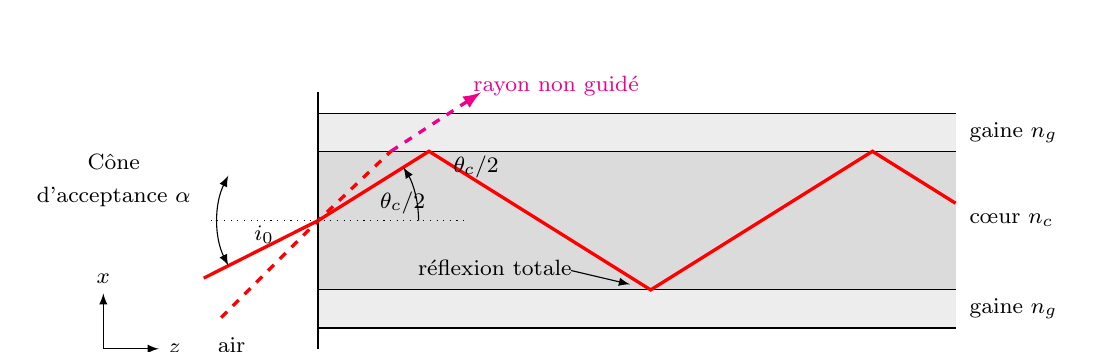
\begin{tikzpicture}[>=latex,scale=0.88]
    % cladding
    \fill[black!7] (1.2,1) rectangle (10.4,1.55);
    \fill[black!7] (1.2,-1.55) rectangle (10.4,-1);
    % core
    \fill[black!14] (1.2,-1) rectangle (10.4,1);
    \draw (1.2,1) -- (10.4,1);
    \draw (1.2,-1) -- (10.4,-1);
    \draw (1.2,1.55) -- (10.4,1.55);
    \draw (1.2,-1.55) -- (10.4,-1.55);
    % input face
    \draw[thick] (1.2,-1.85) -- (1.2,1.85);
    % guided ray
    \draw[very thick,red] (1.2,0) -- (2.8,1) -- (6.0,-1) -- (9.2,1) -- (10.4,0.25);
    % incoming ray inside the acceptance cone
    \draw[very thick,red] (-0.45,-0.83) -- (1.2,0);
    % non guided ray
    \draw[very thick,red,dashed] (-0.2,-1.4) -- (1.2,0) -- (2.25,1);
    \draw[very thick,magenta,dashed,->] (2.25,1) -- (3.55,1.85);
    % acceptance cone
    \draw[<->] ([shift=(206.6:1.45)]1.2,0) arc (206.6:153.4:1.45);
    \draw[dotted] (-0.35,0) -- (3.3,0);
    \node[align=center] at (-1.75,0.58)
      {\footnotesize Cône\\ \footnotesize d'acceptance $\alpha$};
    \node at (0.42,-0.2) {\footnotesize $i_0$};
    % labels
    \draw[->] ([shift=(0:1.45)]1.2,0) arc (0:32:1.45);
    \node at (2.42,0.26) {\footnotesize $\theta_c/2$};
    \node at (3.48,0.78) {\footnotesize $\theta_c/2$};
    \node[right] at (10.46,1.27) {\footnotesize gaine $n_g$};
    \node[right] at (10.46,0) {\footnotesize cœur $n_c$};
    \node[right] at (10.46,-1.27) {\footnotesize gaine $n_g$};
    \node at (-0.05,-1.8) {\footnotesize air};
    \node[magenta,right] at (3.3,1.95) {\footnotesize rayon non guidé};
    \node at (3.75,-0.68) {\footnotesize réflexion totale};
    \draw[->] (4.85,-0.72) -- (5.7,-0.92);
    % axes
    \draw[->] (-1.9,-1.85) -- (-1.9,-1.05) node[above] {\footnotesize $x$};
    \draw[->] (-1.9,-1.85) -- (-1.1,-1.85) node[right] {\footnotesize $z$};
  \end{tikzpicture}
\end{figure}

\begin{remark}[Ouverture numérique]
  On montre que dans une fibre optique $\theta_{\max} \approx \sqrt{2\Delta}$,
  where $\theta_{\max}$ is the largest angle to the axis $0z$ a ray may make
  \emph{inside} the cœur and still stay guided (it is $\theta_c/2$ to first
  order in $\Delta$). Cette valeur est appelée \textbf{ouverture numérique}
  (\textit{numerical aperture}, ON) --- loosely, since the ouverture numérique
  proper is the sine of the largest incidence in air, which is larger by a
  factor of the index of the cœur.
\end{remark}

\begin{remark}
  Dans un guide plan, les rayons se propagent dans le plan $x$--$z$. Cela
  signifie que l'énergie lumineuse sera effectivement piégée dans la couche
  dans le plan vertical mais \emph{pas} dans le plan horizontal supposé infini
  dans la direction $y$. Le faisceau qu'on injecterait dans un tel guide
  continuerait de s'élargir par diffraction dans le plan de la couche.
\end{remark}

\subsubsection{Profil d'indice}
\begin{definition}[Profil d'indice]
  Le \textbf{profil d'indice} (\textit{index profile}) d'un guide définit la
  variation transverse de l'indice, selon la direction $x$ dans notre cas. Un
  guide est complètement défini par son profil d'indice.
\end{definition}

Le plus simple à fabriquer est le profil à saut d'indice dans lequel la fibre
est constituée de deux zones concentriques homogènes avec un saut brutal
d'indice à l'interface cœur/gaine. De nombreux autres profils existent suivant
les applications visées --- depressed gaine, raised gaine, triangular
cœur. Un exemple de profil d'indice typique, a convenient family covering the
cases of interest, peut être donné par l'expression ci-dessous :
\begin{equation*}
  \begin{cases}
    n^2(x) = n_0^2\left[1 - 2\Delta\left(\dfrac{x}{a}\right)^{\alpha}\right]
      & \text{for } |x| < a,\\[2ex]
    n^2(x) = n_0^2\left[1 - 2\Delta\right] & \text{for } |x| > a,
  \end{cases}
\end{equation*}
avec $\alpha \in \reals^{+}$. On constate que ce profil est de forme
triangulaire si $\alpha = 1$, parabolique si $\alpha = 2$, et à saut d'indice si
$\alpha \rightarrow \infty$.

\begin{figure}[h!]
  \centering
  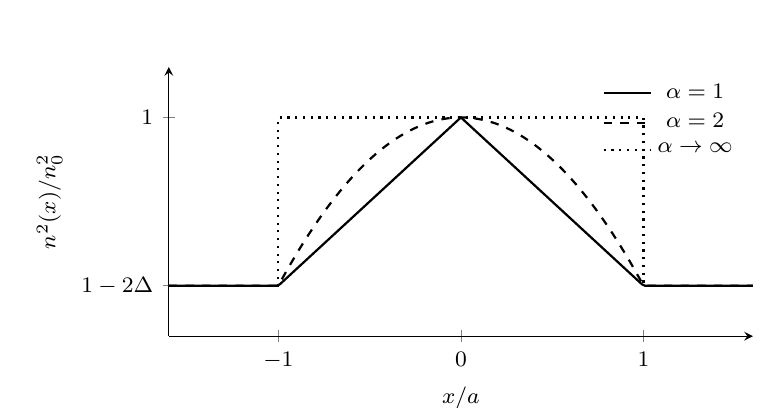
\begin{tikzpicture}
    \begin{axis}[
      width=9cm, height=5cm,
      xlabel={$x/a$}, ylabel={$n^2(x)/n_0^2$},
      xmin=-1.6, xmax=1.6, ymin=0.87, ymax=1.03,
      ytick={0.9,1}, yticklabels={$1-2\Delta$,$1$},
      xtick={-1,0,1}, xticklabels={$-1$,$0$,$1$},
      legend style={at={(0.99,0.98)},anchor=north east,draw=none,fill=none,
                    font=\footnotesize},
      tick label style={font=\footnotesize},
      label style={font=\footnotesize},
      axis lines=left,
      ]
      \addplot[thick,domain=-1.6:1.6,samples=201]{1-0.1*min(abs(x),1)};
      \addlegendentry{$\alpha=1$}
      \addplot[thick,dashed,domain=-1.6:1.6,samples=201]{1-0.1*(min(abs(x),1))^2};
      \addlegendentry{$\alpha=2$}
      \addplot[thick,dotted] coordinates
        {(-1.6,0.9) (-1,0.9) (-1,1) (1,1) (1,0.9) (1.6,0.9)};
      \addlegendentry{$\alpha\rightarrow\infty$}
    \end{axis}
  \end{tikzpicture}
\end{figure}

\noindent (The vertical scale is exaggerated; in a real fibre $2\Delta$ is a
fraction of a percent.) On peut déterminer, par l'approche des rayons, la
trajectoire des rayons lumineux dans la fibre. Cette trajectoire (forme,
période, amplitude…) dépend de nombreux paramètres : profil d'indice transverse
de la fibre, taille transverse du guide, longueur d'onde, angle d'incidence.
Ainsi, on peut trouver des trajectoires en dents de scie dans un guide à saut
d'indice ou des trajectoires sinusoïdales dans un guide à profil parabolique.
Les trajectoires au sein d'un même guide peuvent être multiples dans les guides
multimodes ou unique dans les guides \textbf{monomodes}
(\textit{single-mode}).\\

Le problème est que le temps de trajet dans la fibre dépend de la trajectoire.
Naturellement, s'il existe différentes trajectoires possibles, la lumière
injectée dans la fibre se répartit sur chacune d'entre elles.

\subsubsection{Influence de la dispersion intermodale sur une communication optique}
Une transmission optique numérique consiste à injecter dans la fibre, dans le
cas le plus simple, un signal modulé temporellement en amplitude (ON/OFF).
Après propagation et détection, le signal est remis en forme. Cependant, après
l'injection, la lumière se propage en empruntant les différents chemins
possibles. Après une propagation sur une longueur $L$, l'information qui a
emprunté chaque chemin arrive à des instants différents. Ceci provoque un
élargissement des créneaux. Quand la distance $L$ est trop grande ou le débit
trop important, après remise en forme du signal, celui-ci n'est plus identique
au signal initial, l'information peut être entachée d'erreurs voire
complètement perdue !

\begin{definition}[Dispersion intermodale]
  Ce phénomène de multi-trajets appelé \textbf{dispersion intermodale}
  (\textit{intermodal dispersion}) engendre une limite du débit maximum
  possible --- la \textbf{bande passante} (\textit{bandwidth}) --- sur une
  distance donnée ou réciproquement de la portée de la fibre pour un débit
  donné.
\end{definition}

Si on considère que, pour ne pas commettre d'erreurs à la détection, l'écart
temporel $\Delta\tau$ entre la trajectoire la plus lente et celle la plus rapide
ne doit pas dépasser un quart du \textbf{temps bit} (\textit{bit time})
$T_{\text{bit}}$ avant détection (critère arbitraire --- but a standard one), on
peut en déduire le temps bit minimum (c'est-à-dire la période minimale de
modulation) et donc le débit maximum autorisé sur une fibre :
$T_{\text{bit}} > 4\,\Delta\tau$, soit un \textbf{débit binaire}
(\textit{bit rate}) max acceptable de l'ordre de $1/T_{\text{bit}}$.

\begin{example}[One kilometre of fibre]
  Pour une fibre de $L = 1$\,km,
  \[
    \Delta\tau_{\text{saut d'indice}} = 50\,\mathrm{ns}
    \;\Rightarrow\; T_{\text{bit}} > 200\,\mathrm{ns}
    \;\Rightarrow\; D_{\max} \approx 5\,\mathrm{Mb/s},
  \]
  \[
    \Delta\tau_{\text{parabolique}} = 0{,}25\,\mathrm{ns}
    \;\Rightarrow\; T_{\text{bit}} > 1\,\mathrm{ns}
    \;\Rightarrow\; D_{\max} \approx 1\,\mathrm{Gb/s}.
  \]
  More than two orders of magnitude at stake, on nothing but the shape of the
  profil d'indice.
\end{example}

\begin{remark}[Orders of magnitude]
  Over 1\,km the spread for a saut d'indice profile is
  $\Delta\tau_{\text{saut d'indice}} = 50$\,ns,
  hence $D_{\max} \approx 5$\,Mb/s, while the parabolic profile gives
  $0{,}25$\,ns and $1$\,Gb/s. The ratio of roughly $200$ between the two
  profiles, and the orders of magnitude ``tens of ns'' against ``a fraction of
  a ns'', are what matter in this course.
\end{remark}

\paragraph{Solutions pour s'affranchir de la dispersion intermodale} There are
two.

La première est de modifier le profil d'indice, par exemple en utilisant un
profil à \textbf{gradient d'indice} (\textit{graded index}) où l'indice décroît
au fur et à mesure que l'on s'éloigne du centre de la fibre. La vitesse de la
lumière étant inversement proportionnelle à l'indice de réfraction, le signal
s'accélère lorsque le rayon s'éloigne du centre. Ainsi, bien que les rayons de
plus grande inclinaison aient des trajectoires physiques plus longues, ils se
déplacent plus vite en dehors du centre de la fibre que pour une fibre à saut
d'indice, ce qui réduit la différence de temps de trajets entre les
trajectoires les plus longues et la trajectoire la plus courte. L'influence de
la dispersion modale s'en trouve réduite.\\

La deuxième solution est de limiter le nombre de trajectoires en fabriquant une
fibre monomode où une seule trajectoire --- la plus rapide ! --- est permise.
La suite explique ce qu'est un mode, son lien avec la trajectoire dans la fibre
et comment en limiter le nombre.

\subsection{Notion de mode transverse par approche interférentielle}

Jusqu'à présent, nous avons raisonné avec une approche géométrique. Cependant,
nous avons omis l'aspect ondulatoire de la lumière. Or, puisque des faisceaux
se croisent, il y a certainement des interférences. Le but est de déterminer la
répartition d'énergie dans un plan transverse au guide : cette répartition
est-elle uniforme dans le cœur, à l'image de l'indice, ou présente-t-elle des
modulations ? The answer is that parmi toutes les trajectoires décrites
précédemment, seules certaines sont permises. Les autres sont interdites et ne
se propagent pas. \emph{Les angles permis sont donc quantifiés.}

\subsubsection{Guide plan idéal : guide composé de deux miroirs plans sans pertes}
Three simplifying hypotheses. First, une fibre à symétrie de révolution
engendre des calculs relativement compliqués, et les trajectoires peuvent
potentiellement être hélicoïdales suivant la manière dont on y injecte la
lumière --- des \textbf{rayons hélicoïdaux} (\textit{helical rays}). Nous nous
limiterons à l'étude des \textbf{rayons méridiens} (\textit{meridional rays}),
un rayon méridien étant confiné sur un plan méridien à l'intérieur d'un
cylindre dont le diamètre est celui du cœur ; pour le guide plan, nous nous
limiterons donc aux rayons dans le plan $x$--$z$. Second, nous allons étudier
la propagation d'une onde entre deux miroirs plans, infinis suivant la
direction $y$, séparés d'une distance $D_{\text{cœur}} = 2a$, supposés sans
pertes. Third, on associe à chaque rayon lumineux une onde électromagnétique
transverse plane (TEM selon la direction du rayon). Le champ électromagnétique
total est la somme de ces ondes planes. L'onde est polarisée dans la direction
$y$ et son vecteur d'onde reste dans le plan $x$--$z$.

Un rayon de lumière faisant un angle $\theta/2$ avec le miroir supérieur se
réfléchit puis se propage avec un angle $-\theta/2$ jusqu'au miroir inférieur,
puis se réfléchit, etc. Puisque le vecteur champ électrique est parallèle aux
miroirs, chaque réflexion s'accompagne d'un déphasage $\pi$ pour un miroir
parfait, sans que ni l'amplitude, ni la polarisation ne varient. (The $\pi$ is
dropped in without proof here: un véritable parachutage ! Les plus curieux iront regarder dans la littérature la notion de facteur de
réflexion de Fresnel.)

\subsubsection{Interférences dans le guide : condition de guidage idéale dans un guide plan à miroir parfait}
Si deux ondes cohérentes se superposent en phase, elles s'ajoutent. Par contre,
si elles sont en opposition de phase, elles se soustraient, générant des
interférences destructives et donc de l'obscurité. Si on reprend le modèle de
la propagation des rayons par réflexion totale interne, dans une approche
ondulatoire, on peut remplacer les rayons par des ondes planes. Elles sont
représentées par des traits parallèles, perpendiculaires à la direction de
propagation, qui représentent les plans équiphases. Le principe du guidage de la lumière est que son énergie
doit rester confinée dans le cœur et se conserver lors de la propagation. Ce
qui revient à considérer que l'onde après deux réflexions doit être en phase
avec l'onde initiale modulo $2\pi$ pour rester en interférence constructive et
continuer de se propager.

\begin{figure}[h!]
  \centering
  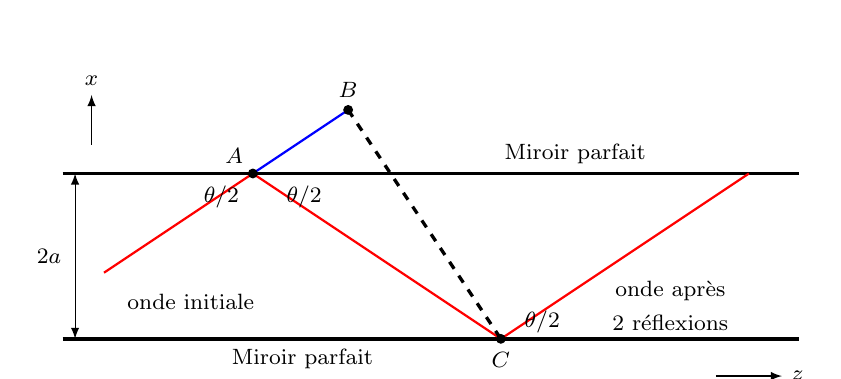
\begin{tikzpicture}[>=latex,scale=1.05]
    % mirrors
    \draw[very thick] (-0.3,1) -- (8.6,1);
    \draw[very thick] (-0.3,-1) -- (8.6,-1);
    \node[above] at (5.9,1) {\footnotesize Miroir parfait};
    \node[below] at (2.6,-1) {\footnotesize Miroir parfait};
    % core width arrow
    \draw[<->] (-0.15,-1) -- (-0.15,1);
    \node[left] at (-0.2,0) {\footnotesize $2a$};
    % initial ray up to A, A to C, C onwards
    \draw[thick,red] (0.2,-0.20) -- (2,1);
    \draw[thick,red] (2,1) -- (5,-1);
    \draw[thick,red] (5,-1) -- (8,1);
    % wavefront BC
    \draw[very thick,dashed] (3.153,1.769) -- (5,-1);
    % AB segment
    \draw[thick,blue] (2,1) -- (3.153,1.769);
    % points
    \fill (2,1) circle (1.7pt);      \node[above left] at (2,1) {\footnotesize $A$};
    \fill (3.153,1.769) circle (1.7pt); \node[above] at (3.153,1.8) {\footnotesize $B$};
    \fill (5,-1) circle (1.7pt);     \node[below] at (5,-1.05) {\footnotesize $C$};
    % angles
    \node at (1.62,0.72) {\footnotesize $\theta/2$};
    \node at (2.62,0.72) {\footnotesize $\theta/2$};
    \node at (5.5,-0.8) {\footnotesize $\theta/2$};
    % annotations
    \node[align=center] at (7.05,-0.6)
      {\footnotesize onde après\\ \footnotesize 2 réflexions};
    \node at (1.25,-0.55) {\footnotesize onde initiale};
    \draw[->] (7.6,-1.45) -- (8.4,-1.45) node[right] {\footnotesize $z$};
    \draw[->] (0.05,1.35) -- (0.05,1.95) node[above] {\footnotesize $x$};
  \end{tikzpicture}
\end{figure}

En termes de déphasage, counting the two reflections as $-2\pi$,
\begin{equation*}
  \Delta\varphi = \frac{2\pi}{\lambda}\,n_c\,(AC - AB) - 2\pi = 2\pi q,
  \qquad q = 0,1,2,3,\dots
\end{equation*}
Ainsi, les deux ondes se séparant au point $A$ doivent chacune avoir parcouru
des chemins optiques jusqu'aux points $B$ et $C$ tels que leur différence doit
être un multiple de la longueur d'onde :
\begin{equation*}
  n_c\,(AC - AB) = (q+1)\lambda = m\lambda, \qquad m = 1,2,3,\dots
\end{equation*}
With $a$ the half-width of the guide, trigonometry gives
\begin{equation*}
  AB = AC\cos\theta \qquad\text{and}\qquad AC = \frac{2a}{\sin\theta/2},
\end{equation*}
and there remains the \textbf{condition de guidage} (\textit{guiding
condition}) itself.

\begin{theorem}[Condition de guidage idéale dans un guide plan à miroir parfait]
  \begin{equation*}
    D_{\text{cœur}} = 2a = m\,\frac{\lambda}{2n_c\sin\dfrac{\theta}{2}},
    \qquad m = 1,2,3,\dots
  \end{equation*}
\end{theorem}

Cette condition de guidage relie les paramètres physiques du guide (diamètre,
indice) aux paramètres de l'onde y circulant (longueur d'onde et angle). Cette
équation peut être vue de différentes manières : pour un guide donné ($n_c$ et
$a$ fixés), on peut étudier pour une longueur d'onde donnée quels sont les
angles permis dans le guide ; pour un guide donné, on peut étudier quelles
longueurs d'onde sont permises dans le guide ; on peut enfin choisir
\emph{a priori} les modes et les longueurs d'onde que l'on souhaite voir se
propager dans le guide et fabriquer la fibre en fonction.

\subsubsection{Modes guidés = angles permis et quantifiés}
Prenons le cas d'une lumière monochromatique de longueur d'onde $\lambda$ se
propageant dans la fibre. Dans l'expression de la condition de guidage, on
constate que pour $a$, $n_c$ et $\lambda$ fixés, il existe un angle donné
$\theta_m$ pour chaque entier $m$ pour que la condition de guidage soit
satisfaite :
\begin{equation*}
  \boxed{\;\frac{\theta_m}{2}
    = \sin^{-1}\!\left(m\,\frac{\lambda}{2 D_{\text{cœur}} n_c}\right)\;}
\end{equation*}

\begin{conclusion}
  Les angles des rayons dont l'énergie est guidée sont \emph{quantifiés}.
  Seuls certains sont permis. Les autres ne se propagent pas, \emph{même s'ils
  satisfont la condition de réflexion totale interne}. Un \textbf{mode guidé}
  (\textit{guided mode}) correspond donc à un angle de propagation dans le
  guide.
\end{conclusion}

\begin{example}[Application numérique]
  Prenons un guide de rayon $a = 4{,}5\,\mu$m (soit $D_{\text{cœur}} =
  9\,\mu$m) dans lequel se propage une lumière de longueur d'onde
  $\lambda = 1{,}55\,\mu$m :
  \[
    \begin{array}{llll}
      m = 1: & \theta_1/2 = 3{,}38^\circ \qquad&
      m = 2: & \theta_2/2 = 6{,}77^\circ \\
      m = 3: & \theta_3/2 = 10{,}19^\circ \qquad&
      m = 4: & \theta_4/2 = 13{,}64^\circ \\
      m = 5: & \theta_5/2 = 17{,}15^\circ &&
    \end{array}
  \]
  Il est également important de noter que chaque angle dépend de $\lambda$.
\end{example}

\begin{remark}[Checking the list]
  Each entry is the boxed formula evaluated directly: for $m = 1$ it gives
  $\theta_1/2 = 3{,}38^\circ$, and the later angles stay close to whole
  multiples of it, the sine being still nearly linear at these angles.
\end{remark}

\subsubsection{Distribution transverse d'intensité}
Pour un angle donné, des ondes vont se propager à la fois vers le haut avec un
angle $\theta$ et vers le bas avec un angle $-\theta$ et vont donc se croiser.
Ces ondes issues de la même source sont cohérentes et vont donc interférer. Le
déphasage entre les deux ondes planes est
\begin{equation*}
  \Delta\varphi = \varphi_2 - \varphi_1
    = \frac{4\pi}{\lambda}\,n_c\,x\,\sin\frac{\theta}{2},
\end{equation*}
et des interférences constructives se forment lorsque $\Delta\varphi$ est un
multiple de $2\pi$. Cette figure d'interférence est constituée de franges
sinusoïdales parallèles au plan $y0z$, elle ne dépend que de $x$, est
indépendante de $y$ et de $z$. Plus l'angle entre les deux ondes est grand,
plus l'interfrange est petit.\\

On pourrait montrer que les angles permis correspondent à des situations où
les interférences sont \emph{destructives sur les miroirs}. S'il n'y a pas
d'énergie aux interfaces, la lumière reste guidée. Sinon, la lumière n'est plus
guidée car une partie de l'énergie fuit dans la gaine au fur et à mesure des
réflexions successives.

\begin{figure}[h!]
  \centering
  \foreach \m in {1,2,3,4}{%
    \begin{tikzpicture}
      \begin{axis}[
        width=4.0cm, height=3.6cm,
        xmin=-1.05, xmax=1.05, ymin=-0.06, ymax=1.15,
        xtick={-1,1}, xticklabels={$-a$,$a$},
        ytick=\empty,
        xlabel={\footnotesize $x$},
        title={\footnotesize $m=\m$},
        tick label style={font=\footnotesize},
        axis lines=left, axis line style={-},
        ]
        \addplot[thick,domain=-1:1,samples=161]
          {sin(\m*90*(x+1))^2};
      \end{axis}
    \end{tikzpicture}\hfill}
\end{figure}

Chaque mode peut être vu comme une onde stationnaire dans la direction $x$, se
propageant dans la direction $z$. Le nombre $m$ représente le nombre de franges
visibles entre les deux miroirs ; on l'appellera l'\textbf{ordre du mode}
(\textit{order of the mode}). La répartition transverse d'intensité suivant $x$
sera donc sinusoïdale dans le cœur, s'annulant sur les miroirs.

\begin{definition}[Mode transverse]
  Un \textbf{mode transverse} (\textit{transverse mode}) guidé correspond à un
  angle de propagation dans le guide \emph{et} une répartition transverse
  donnée. Un mode transverse est un champ qui maintient sa répartition
  transverse et sa polarisation suivant la direction de propagation $z$.
\end{definition}

\begin{remark}
  $m = 0$ ne fournissant pas de solution, il n'est pas permis ! This changes
  once the mirrors are replaced by real dielectric interfaces.
\end{remark}

\subsubsection{Nombre de modes guidés}
Un sinus étant toujours inférieur à $1$, on peut écrire
\begin{equation*}
  \sin\frac{\theta_m}{2} = m\,\frac{\lambda}{2D_{\text{cœur}}n_c} < 1
  \qquad\Longrightarrow\qquad
  m < \frac{2D_{\text{cœur}}n_c}{\lambda},
\end{equation*}
et le nombre de modes guidés peut donc s'écrire
\begin{equation*}
  \boxed{\;m_{\max} \le E\!\left[\frac{2D_{\text{cœur}}n_c}{\lambda}\right]\;}
\end{equation*}
où $E[\,\cdot\,]$ représente la partie entière. Le nombre de modes augmente
avec le rapport $2D_{\text{cœur}}n_c/\lambda$ :
\begin{itemize}
  \item si $2D_{\text{cœur}}n_c/\lambda < 1$, aucun mode ne peut se propager ;
  \item si $1 < 2D_{\text{cœur}}n_c/\lambda < 2$, seul le mode fondamental
    $m = 1$ peut se propager. Le guide est dit monomode transverse.
\end{itemize}

\begin{example}
  Reprenons un guide d'épaisseur $9\,\mu$m dans lequel se propage une lumière
  de longueur d'onde $\lambda = 1{,}55\,\mu$m. Alors, le nombre maximum de
  modes pouvant se propager est $m < 16{,}95$ : seuls $16$ modes peuvent se
  propager dans ce guide \emph{idéal}. Bizarre, le guide n'est pas monomode ---
  yet the SMF28 is supposed to be monomode at that longueur d'onde. The
  perfect-mirror model is missing something, and what it is missing is
  réflexion totale interne.
\end{example}

\subsubsection{Constante de propagation}
\begin{remark}
  \textit{Pour aller plus loin} --- this subsection and the next go beyond the
  main line of this course.
\end{remark}

In the cœur the vecteur d'onde has norm $n_c k_0$, and its component along $x$ is
\begin{equation*}
  k_{xm} = n_c k_0 \sin\!\left(\frac{\theta_m}{2}\right)
         = m\,\frac{\pi}{D_{\text{cœur}}},
  \qquad \|\v{k}_0\| = \frac{2\pi}{\lambda}.
\end{equation*}
Une onde guidée se compose de deux ondes planes distinctes se propageant dans
le plan $x$--$z$, faisant un angle $\pm\theta/2$ avec l'axe $z$. Ses vecteurs
d'onde ont des composantes $(k_x,0,k_z)$ et $(-k_x,0,k_z)$. Leur somme ou leur
différence varie selon $z$ en $\exp(-jk_z z)$. On peut alors dire que la
constante de propagation suivant $z$ d'une onde guidée est
$\gamma \equiv k_z = n_c k_0\cos\theta/2$. Ainsi, $\gamma$ est quantifié :
\begin{equation*}
  \gamma_m = n_c k_0\cos\!\left(\frac{\theta_m}{2}\right),
  \qquad
  \gamma_m^2 = n_c^2 k_0^2\cos^2\!\left(\frac{\theta_m}{2}\right)
             = n_c^2 k_0^2\left(1-\sin^2\!\left(\frac{\theta_m}{2}\right)\right),
\end{equation*}
\begin{equation*}
  \boxed{\;\gamma_m^2 = n_c^2 k_0^2
    - \left(m\,\frac{\pi}{D_{\text{cœur}}}\right)^2\;}
\end{equation*}

\begin{figure}[h!]
  \centering
  \begin{tikzpicture}[>=latex,scale=1.0]
    \draw[->] (0,-0.2) -- (0,2.2) node[above] {\footnotesize $x$};
    \draw[->] (-0.2,0) -- (5.2,0) node[right] {\footnotesize $z$};
    \draw[very thick,red,->] (0,0) -- (4.2,1.7)
      node[above right] {\footnotesize $n_c\v{k}_0$};
    \draw[thick,blue,->] (0,0) -- (0,1.7)
      node[midway,left] {\footnotesize $k_{xm}$};
    \draw[thick,blue,->] (0,0) -- (4.2,0)
      node[midway,below] {\footnotesize $k_z = \gamma$};
    \draw[dashed] (4.2,0) -- (4.2,1.7) -- (0,1.7);
    \draw[->] (1.0,0) arc (0:22:1.0);
    \node at (1.32,0.20) {\footnotesize $\theta_m/2$};
  \end{tikzpicture}
\end{figure}

On constate que $\gamma_m$ varie avec $m$. $\gamma$ étant reliée à la vitesse
de propagation des modes suivant $z$, chaque mode se déplace à une vitesse
différente des autres --- cohérent avec le fait que les longueurs de
trajectoires ne soient pas les mêmes, and the wave-optics face of the
dispersion intermodale.

\subsubsection{Équation de dispersion}
\begin{definition}[Équation de dispersion]
  La relation entre la constante de propagation $\gamma$ et la fréquence
  angulaire $\omega$ est une relation caractéristique importante d'un guide,
  connue sous le nom d'\textbf{équation de dispersion} (\textit{dispersion
  equation}).
\end{definition}
Pour un milieu homogène infini, la relation est simple et s'exprime comme
$\omega = c\gamma/n$, with $n$ the medium's index. Pour le mode $m$ d'un guide
plan à miroir parfait, whose cœur has index $n_c$,
\begin{equation*}
  \gamma_m^2 = \frac{n_c^2\omega^2}{c^2}
    - \left(m\,\frac{\pi}{D_{\text{cœur}}}\right)^2 .
\end{equation*}
Pour le guide diélectrique, et \emph{a fortiori} pour la fibre optique à
symétrie de révolution, cette équation de dispersion (et donc sa résolution)
est beaucoup plus complexe et n'admet pas de solution analytique.

\subsection{Guide plan diélectrique}

On considère cette fois un \textbf{guide plan diélectrique} (\textit{dielectric
plane guide}), c'est-à-dire un milieu d'indice $n_c$ entouré par un milieu
d'indice $n_g$. La réflexion a donc lieu sur les dioptres cœur/gaine et non plus
sur des miroirs parfaits.

\subsubsection{Nombre de modes guidés}
À la différence d'un miroir parfait qui réfléchit identiquement quel que soit
l'angle d'incidence, pour un diélectrique, la réflexion dépend de l'angle et il
existe un angle limite pour lequel la réflexion n'est plus totale. Cela
introduit une condition angulaire de guidage par réflexion totale interne, on
top of the interference condition :
\begin{equation*}
  \frac{\theta_m}{2} < \frac{\theta_c}{2}
  = \frac{\pi}{2} - i_c
  = \frac{\pi}{2} - \sin^{-1}\!\left(\frac{n_g}{n_c}\right)
  = \cos^{-1}\!\left(\frac{n_g}{n_c}\right),
\end{equation*}
soit $\sin^{-1}\!\left(m\lambda/2D_{\text{cœur}}n_c\right) <
\cos^{-1}(n_g/n_c)$.

\begin{theorem}[Modes guidés d'un guide plan diélectrique]
  A mode $m$ is guided if and only if
  \begin{equation*}
    m < \frac{2D_{\text{cœur}}n_c}{\lambda}\,
        \sin\!\left(\cos^{-1}\!\left(\frac{n_g}{n_c}\right)\right).
  \end{equation*}
\end{theorem}

Bien que certains modes puissent a priori être guidés dans une structure à
miroirs parfaits, dans un guide diélectrique, si ces modes ne satisfont pas la
condition de réflexion totale, ils s'annulent au fur et à mesure de la
propagation en subissant des pertes à chaque réflexion.

\begin{example}[SMF28 revisited]
  Avec $D_{\text{cœur}} = 9\,\mu$m (dimensions d'une fibre monomode standard
  SMF28) :
  \begin{subpart}
    \item Si $\lambda = 1{,}55\,\mu$m, $m < 1{,}4$ : seul le mode fondamental
      $m = 1$ faisant un angle $\theta_1/2$ par rapport à $z$ est guidé. Le
      guide est dit monomode. Ceci correspond bien à l'application numérique
      précédente où l'on constate que $\theta_2/2 = 6{,}77^\circ$ est
      supérieur à l'angle limite de RTI $\theta_c/2 = 4{,}74^\circ$. Compare
      the perfect-mirror answer, $16$ modes.
    \item Si cette fibre monomode dans l'IR est utilisée dans le violet
      ($\lambda = 0{,}4\,\mu$m), alors $m < 5{,}42$ : 5 modes peuvent se
      propager, les modes $m = 1,2,3,4,5$.
  \end{subpart}
\end{example}

\begin{conclusion}[Ajustement du nombre de modes]
  Pour ajuster le nombre de modes transverses guidés, on peut jouer sur la
  longueur d'onde $\lambda$, la taille de guide $D_{\text{cœur}} = 2a$ et
  l'angle limite $\theta_c/2$ (en jouant sur $n_c$ et $n_g$) : plus
  $\lambda$ diminue, plus $m$ augmente ; plus $D_{\text{cœur}}$ diminue, plus
  $m$ diminue ; plus $\theta_c/2$ diminue, plus $m$ diminue. Donc, pour rendre
  le guide monomode, il faut diminuer la taille du guide ou diminuer
  $\theta_c/2$ (en augmentant $n_g$ par rapport à $n_c$).
\end{conclusion}

\subsubsection{Longueur d'onde de coupure}
On sait que pour qu'un mode soit guidé, il faut remplir la condition
$\theta_m/2 < \theta_c/2$. Read the other way round, pour un mode donné $m$,
dans un guide donné ($a$, $n_c$ et $n_g$ fixés), on peut définir une condition
sur la longueur d'onde pour l'existence d'un mode :
\begin{equation*}
  \boxed{\;\lambda < \lambda_{cm}
    = \frac{2D_{\text{cœur}}n_c}{m}\,
      \sin\!\left(\cos^{-1}\!\left(\frac{n_g}{n_c}\right)\right)\;}
\end{equation*}

\begin{example}[Application numérique]
  For the same guide,
  \[
    \lambda_{C1} = 2{,}17\,\mu\mathrm{m},\quad
    \lambda_{C2} = 1{,}08\,\mu\mathrm{m},\quad
    \lambda_{C3} = 0{,}72\,\mu\mathrm{m},\quad
    \lambda_{C4} = 0{,}54\,\mu\mathrm{m},\quad
    \lambda_{C5} = 0{,}43\,\mu\mathrm{m}.
  \]
  Le mode $1$ existe si $\lambda < 2{,}17\,\mu$m, le mode $2$ si
  $\lambda < 1{,}08\,\mu$m, etc. Le guide est donc monomode si la longueur
  d'onde $\lambda$ est comprise entre $\lambda_{C2}$ et $\lambda_{C1}$, soit
  \[
    1{,}08\,\mu\mathrm{m} < \lambda < 2{,}17\,\mu\mathrm{m}.
  \]
  Pour $\lambda = 0{,}4\,\mu$m, on retrouve bien que 5 modes se propagent car
  $\lambda < \lambda_{C5}$.
\end{example}

\subsubsection{Correction du modèle utilisé}
Dans le modèle précédent du guide diélectrique, nous avons omis le fait que,
lorsque $n_c > n_g$ et que $\theta/2 < \theta_c/2$, c'est-à-dire que l'on se
place dans le cas de la réflexion totale, la réflexion d'une onde fait
apparaître un déphasage $\varphi_r(\theta/2)$ --- no longer $\pi$ ---
relativement complexe qui dépend de l'angle d'incidence $\theta/2$ \emph{et}
de la polarisation de l'onde (coefficients de Fresnel). Il convient alors de
distinguer deux types de polarisation :
\begin{itemize}
  \item \textbf{Mode TE} (Transverse Électrique) : le champ
    électrique est polarisé perpendiculairement au plan $x$--$z$ ;
  \item \textbf{Mode TM} (Transverse Magnétique) : le champ
    magnétique est polarisé perpendiculairement au plan $x$--$z$.
\end{itemize}
The round-trip phase condition
$\Delta\varphi = (4\pi/\lambda)\,n_c\,x\,\sin(\theta/2) + 2\pi$ devient
\begin{equation*}
  \Delta\varphi = \frac{4\pi}{\lambda}\,n_c\,x\,\sin\frac{\theta}{2}
    + 2\varphi_r\!\left(\frac{\theta}{2}\right) = 2m\pi,
  \qquad m = 0,1,2,3,\dots
\end{equation*}

Three consequences follow. La condition de guidage est alors différente du
guide à miroir parfait et diffère suivant la polarisation étudiée ; elle
aboutit à l'expression d'une \emph{équation transcendante}, appelée équation
de dispersion, qui ne possède pas de solution analytique. La résolution est
numérique ou graphique et permet de trouver les angles permis dans le guide.
Les miroirs n'étant plus parfaits, le champ n'est plus nul aux interfaces : il
est toujours sinusoïdal dans le cœur, mais dans la gaine il prend l'expression
d'une \textbf{onde évanescente} (\textit{evanescent wave}) : le champ décroît
exponentiellement dans la gaine. De plus, contrairement au cas où on ne tient
pas compte de ce déphasage, ici, $m = 0$ est permis. Ceci engendre qu'\emph{il
n'existe pas de longueur d'onde de coupure absolue pour un guide symétrique}.
Le mode $m=0$ se propage toujours. Par contre, $m = 0$ ne correspond pas à
$\theta = 0$ mais au plus petit angle guidé dans le guide.

\begin{figure}[h!]
  \centering
  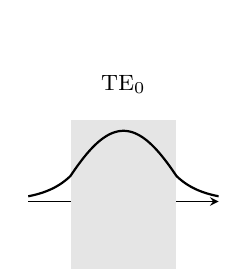
\begin{tikzpicture}
    \begin{axis}[
      width=4.0cm, height=3.6cm,
      xmin=-1.8, xmax=1.8, ymin=-1.1, ymax=1.15,
      xtick=\empty, ytick=\empty,
      title={\footnotesize TE$_0$},
      axis x line=middle, axis y line=none,
      ]
      \fill[black!10] (axis cs:-1,-1.1) rectangle (axis cs:1,1.15);
      \addplot[thick,domain=-1.8:1.8,samples=201]
        {abs(x)<1 ? cos(68.75*x) : 0.362*exp(-2*(abs(x)-1))};
    \end{axis}
  \end{tikzpicture}\hfill
  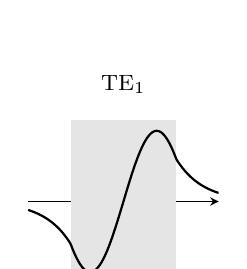
\begin{tikzpicture}
    \begin{axis}[
      width=4.0cm, height=3.6cm,
      xmin=-1.8, xmax=1.8, ymin=-1.1, ymax=1.15,
      xtick=\empty, ytick=\empty,
      title={\footnotesize TE$_1$},
      axis x line=middle, axis y line=none,
      ]
      \fill[black!10] (axis cs:-1,-1.1) rectangle (axis cs:1,1.15);
      \addplot[thick,domain=-1.8:1.8,samples=201]
        {abs(x)<1 ? sin(143.24*x) : ((x>0 ? 0.598 : -0.598)*exp(-2*(abs(x)-1)))};
    \end{axis}
  \end{tikzpicture}\hfill
  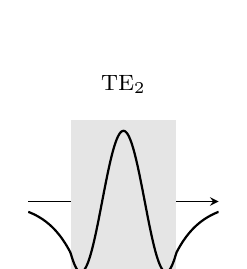
\begin{tikzpicture}
    \begin{axis}[
      width=4.0cm, height=3.6cm,
      xmin=-1.8, xmax=1.8, ymin=-1.1, ymax=1.15,
      xtick=\empty, ytick=\empty,
      title={\footnotesize TE$_2$},
      axis x line=middle, axis y line=none,
      ]
      \fill[black!10] (axis cs:-1,-1.1) rectangle (axis cs:1,1.15);
      \addplot[thick,domain=-1.8:1.8,samples=201]
        {abs(x)<1 ? cos(223.45*x) : -0.726*exp(-2*(abs(x)-1))};
    \end{axis}
  \end{tikzpicture}\hfill
  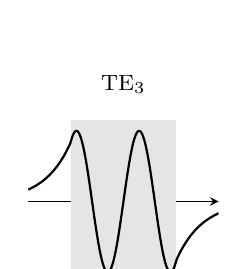
\begin{tikzpicture}
    \begin{axis}[
      width=4.0cm, height=3.6cm,
      xmin=-1.8, xmax=1.8, ymin=-1.1, ymax=1.15,
      xtick=\empty, ytick=\empty,
      title={\footnotesize TE$_3$},
      axis x line=middle, axis y line=none,
      ]
      \fill[black!10] (axis cs:-1,-1.1) rectangle (axis cs:1,1.15);
      \addplot[thick,domain=-1.8:1.8,samples=201]
        {abs(x)<1 ? sin(303.66*x) : ((x>0 ? -0.830 : 0.830)*exp(-2*(abs(x)-1)))};
    \end{axis}
  \end{tikzpicture}
\end{figure}

\noindent The shaded band is the cœur, $|x| < a$. À comparer avec le cas d'un
guide à miroir parfait, where the field is forced to zero exactly on the
mirrors and nothing exists outside the cœur.

\subsection{Résolution formelle à partir des équations de Maxwell}

Si on prend en compte le déphasage à l'interface cœur-gaine pour un guide plan,
le modèle reste complet. Par contre, ce modèle est très difficilement
utilisable dans le cas d'une fibre à symétrie de révolution ! Imaginez les
calculs d'interférences avec des trajectoires hélicoïdales ! Il est
heureusement possible de résoudre ce problème de manière rigoureuse dans le cas
du guide plan aussi bien que dans le cas d'une fibre optique à symétrie de
révolution à partir des équations de Maxwell.

\subsubsection{Cas général}
\begin{postulate}[Les modes propres forment une base]
  L'ensemble des solutions électromagnétiques du problème du guide forme un
  espace vectoriel dont les modes propres forment une base. Une solution
  quelconque pourra donc être représentée comme une combinaison linéaire de
  modes de la structure.
\end{postulate}

Le point de départ est l'équation de propagation pour le champ électrique,
simplifiée parce que l'on considère le milieu diélectrique pur, sans charge ni
courant, mais qui reste valable dans un milieu dont l'indice $n$ varie
lentement sur une longueur égale à la longueur d'onde. Pas de charges :
$\rho = 0$ ; donc, le milieu ne peut générer de courant : $\v{J} = 0$ ; donc sa
conductivité est nulle : $\sigma = 0$. Les équations de Maxwell deviennent
\begin{equation*}
  \begin{cases}
    \curl \v{E} = -\dfrac{\del \v{B}}{\del t}\\[1.6ex]
    \div \v{B} = 0
  \end{cases}
  \qquad
  \begin{cases}
    \curl \v{B} = \varepsilon\mu\dfrac{\del \v{E}}{\del t}\\[1.6ex]
    \div \v{E} = 0
  \end{cases}
\end{equation*}
En éliminant $\v{B}$,
\begin{equation*}
  \curl(\curl \v{E}) = \grad(\div \v{E}) - \Delta \v{E}
    = \varepsilon\mu\frac{\del^2 \v{E}}{\del t^2}
  \qquad\Longrightarrow\qquad
  \varepsilon\mu\frac{\del^2 \v{E}}{\del t^2} - \Delta \v{E} = 0 .
\end{equation*}
Les modes guidés sont les solutions de cette équation, si elles existent, en
forme d'onde progressive le long de l'axe du guide, c'est-à-dire avec une
dépendance en
\begin{equation*}
  \v{E}(\v{r},t) = \v{E}(x)\,e^{i(\omega t - \gamma z)},
\end{equation*}
où $\gamma$ est une quantité a priori inconnue que l'on devra extraire de
l'équation de propagation et qui est appelée constante de propagation (c'est
la même variable que plus haut). Pour une solution sinusoïdale de pulsation $\omega$,
l'équation de propagation devient
\begin{equation*}
  \frac{\del^2 \v{E}(\v{r})}{\del x^2}
  + \frac{\del^2 \v{E}(\v{r})}{\del y^2}
  + \frac{\del^2 \v{E}(\v{r})}{\del z^2}
  + \frac{\omega^2 n^2}{c^2}\,\v{E}(\v{r}) = 0,
\end{equation*}
or, for the plane guide, with the $z$ and $t$ dependence carried by the
exponential,
\begin{equation*}
  \frac{\del^2 \v{E}(x)}{\del x^2}
  + \left(\frac{\omega^2 n^2}{c^2} - \gamma^2\right)\v{E}(x) = 0 .
\end{equation*}
(Il existe les mêmes équations pour le champ magnétique $\v{B}$.) Le principe
est de résoudre cette équation (en coordonnées polaires pour une fibre), dans
les deux régions du guide (cœur et gaine) en établissant des conditions aux
limites qui sont la continuité du champ et de sa dérivée aux interfaces. La
solution générale de l'expression transverse du champ est alors
\begin{equation*}
  \v{E}(x) = \v{A}\,e^{+j\alpha x} + \v{B}\,e^{-j\alpha x},
  \qquad\text{with}\qquad
  \alpha^2 = \frac{\omega^2 n^2}{c^2} - \gamma^2 .
\end{equation*}
En réalité, on cherche un triplet $(\omega,\alpha,\gamma)$ pour lequel
$\v{E}(x)$ est un champ confiné. Pour une fréquence angulaire $\omega$ donnée,
3 cas se présentent car $n$ prend deux valeurs distinctes $n_c$ et $n_g$.

\begin{itemize}
  \item $\gamma > \omega n_c/c > \omega n_g/c$ : $\alpha$ est imaginaire pur et
    le champ est exponentiel dans les trois régions. Pas de réalité physique.
  \item $\omega n_c/c > \gamma > \omega n_g/c$ : le champ est exponentiel
    décroissant dans les régions 1 et 3 et sinusoïdal dans la région 2.
    L'énergie est confinée au voisinage du cœur et fait apparaître une onde
    évanescente dans la gaine.
  \item $\omega n_c/c > \omega n_g/c > \gamma$ : le champ est sinusoïdal dans
    les trois régions. Pas de confinement du champ.
\end{itemize}

\begin{theorem}[Condition d'existence d'un mode guidé]
  La constante de propagation $\gamma$ dans le guide doit être comprise entre
  les deux bornes
  \begin{equation*}
    \frac{\omega n_g}{c} < \gamma < \frac{\omega n_c}{c}
  \end{equation*}
  pour des milieux d'indice $n_g$ et $n_c$ lorsque ces derniers sont illimités.
\end{theorem}

\begin{remark}
  On pourrait montrer que cette condition est identique à la condition de
  réflexion totale $\theta/2 < \theta_c/2$ trouvée précédemment. Cette méthode
  ne permet d'obtenir des solutions analytiques que dans des cas très simples
  (guide plan). Sinon, on doit se contenter d'une résolution graphique pour
  déterminer la valeur de $\gamma$.
\end{remark}

\subsubsection{Résolution dans le cas du guide planaire à saut d'indice}
Dans ce cas, le guide est infini suivant la direction $y$ et l'indice est
constant dans le cœur et dans la gaine. Après quelques simplifications
\[
  \frac{\del}{\del y} = 0 \quad(\text{planar structure}), \qquad
  \frac{\del}{\del z} = -j\beta \quad(\text{propagation along } z), \qquad
  \frac{\del}{\del t} = -j\omega,
\]
on obtient un jeu de 6 équations en $(E_x, E_z, B_y, B_x, B_z, E_y)$. On
constate que les trois premières équations sont indépendantes des 3 dernières.
Les trois premières correspondent au cas TM alors que les 3 dernières
correspondent au cas TE. De ces deux jeux de trois équations, on peut extraire
\begin{equation*}
  \frac{\del^2 E_y(x)}{\del x^2}
    + \left(\frac{\omega^2 n^2}{c^2} - \gamma^2\right) E_y(x) = 0,
  \qquad
  \frac{\del^2 B_y(x)}{\del x^2}
    + \left(\frac{\omega^2 n^2}{c^2} - \gamma^2\right) B_y(x) = 0 .
\end{equation*}
La résolution de ces deux équations et l'application des conditions aux
limites permet de remonter au profil du champ dans le cas TE ou TM, via une
équation de dispersion transcendante comme pour le modèle précédent --- the
corrected interference model. Par exemple, dans le cas TE, on retrouve une
équation de dispersion et une répartition du champ identiques à celles
trouvées dans ce modèle.

\subsubsection{Résolution dans le cas de la fibre}
Pour une fibre à symétrie de révolution, il convient de travailler en
coordonnées polaires. En supposant la continuité de $E$ et de sa dérivée en
$r = a$, si on résout l'équation dans le cas d'une fibre à saut d'indice, on
trouve :
\begin{itemize}
  \item si $r < a$ (cœur), $E$ est une \textbf{fonction de Bessel de première
    espèce} (\textit{Bessel function of the first kind}) ;
  \item si $r > a$ (gaine), $E$ est une \textbf{fonction de Bessel modifiée}
    (\textit{modified Bessel function}).
\end{itemize}
On considère dans un premier temps que le guide est isotrope (invariance par
rotation : pas de différence entre $x$ et $y$). La base de polarisation
linéaire et orthogonale choisie peut être la base $x$ et $y$. Les combinaisons
de modes trouvés sont alors dites de type \textbf{LP} (\textit{Linear
Polarization}) et sont en réalité des solutions approchées.

L'introduction de conditions aux limites fait apparaître une équation de
dispersion, généralement compliquée, qui permet graphiquement de définir
l'existence de telle ou telle solution, comme nous avons pu le constater avec
l'approche géométrique. En réalité, à une dimension (guide plan), le
confinement suivant l'axe $x$ faisait apparaître un et un seul nombre de
quantification $m$. Dans le cas d'une fibre, le confinement est suivant deux
variables, il fait donc apparaître deux nombres quantiques :
\begin{itemize}
  \item suivant le rayon $r$ : confinement à l'intérieur du cœur, un nombre
    quantique $l$ ;
  \item suivant l'angle $\theta$ : après une rotation multiple de $2\pi$, le
    champ doit revenir égal à lui-même, un nombre quantique $m$.
\end{itemize}
Pour $l$ fixé, il existe un nombre fini de solutions de l'équation de
dispersion, $m = 0,1,2,3,\dots$, et le mode correspondant est noté
$\mathrm{LP}_{lm}$. Cette condition d'existence de chaque mode se traduit par
l'apparition de fréquence de coupure comme on l'a vu dans le modèle précédent.
Après injection dans la fibre, la lumière va se répartir suivant les
différents modes pouvant exister (en fonction de la pulsation).

\begin{prop}[Orthogonalité des modes (\textit{orthogonality of the modes})]
  Les modes sont orthogonaux au sens du produit scalaire
  \begin{equation*}
    \int_0^{2\pi}\!\!\int_0^{+\infty}
      \Psi_{lm}\,\Psi^{*}_{l'm'}\;\mathrm{d}r\,\mathrm{d}\theta
    = \begin{cases}
        1 & \text{if } l = l' \text{ and } m = m',\\
        0 & \text{if } l \neq l' \text{ or } m \neq m'.
      \end{cases}
  \end{equation*}
  Un profil d'intensité quelconque se décompose donc sur la base des modes
  propres de la fibre, par exemple
  $a\times \mathrm{LP}_{01} + b\times \mathrm{LP}_{02}
  + c\times \mathrm{LP}_{03}$.
\end{prop}

\begin{remark}[Modes dégénérés]
  Il arrive que l'on puisse avoir deux modes différents avec la même constante
  de propagation $\gamma$. On dit alors qu'ils sont \textbf{dégénérés}
  (\textit{degenerate}). Par exemple, dans une fibre circulaire, une rotation
  de $90^\circ$ autour de l'axe transformera toute solution en une autre
  solution, généralement indépendante de la première mais avec la même
  constante de propagation. Idem pour les solutions paires et impaires, as
  for $\mathrm{LP}_{11}$, $\mathrm{LP}_{12}$, $\mathrm{LP}_{21}$,
  $\mathrm{LP}_{22}$ and $\mathrm{LP}_{31}$.
\end{remark}

\subsection{Performances et domaines d'application}

\begin{conclusion}[Intérêt de la fibre]
  Performance de transmission : très faibles pertes, de l'ordre de
  $0{,}2$\,dB/km ; très grande bande passante, au-delà de $12$\,THz ;
  multiplexage possible sur plusieurs canaux. Mise en œuvre : faible poids,
  faible taille --- gaine de quelques centaines de $\mu$m. Sécurité électrique :
  isolation totale entre terminaux, insensibilité aux parasites électriques
  (n'en crée pas !), possibilité d'utilisation en ambiance explosive,
  applications médicales. Inviolabilité : difficile d'intercepter le signal.
\end{conclusion}

\paragraph{Télécommunications} Il existe près de 300 câbles sous-marins
(environ $885\,000$\,km, $99\%$ des données). Ces câbles font généralement
$8$\,cm de diamètre maximum (pour un poids de $10$\,kg/m), avec plusieurs
fibres par câble fonctionnant par paires (une pour chaque sens de
transmission). Leur débit est proche de $4$\,Tbit/s par paire (200\,000 fois
plus important que le débit d'une connexion ADSL classique).

\paragraph{Imagerie et sources lasers} Imagerie médicale (endoscope, chirurgie
laser) et inspection vidéo ; sources laser de fortes puissances (10\,kW CW),
sources à impulsions ultra-courtes ($< 100$\,fs) et sources larges bandes.

\paragraph{Capteurs distribués} Le principe de base est l'\textbf{OTDR}
(\textit{Optical Time Domain Reflectometer}) : un interrogateur (émission,
détection, traitement des données), and the echo along the fibre locates
events --- a connector, a bend --- by their delay. Two physical effects are
exploited.

In a \textbf{distributed acoustic sensor} (DAS-OTDR), built on Rayleigh
scattering, the pulse illuminates the scattering centres of the $L$th kilometre
of fibre. À un instant donné, on détecte des interférences intra-impulsion à
un endroit :
\begin{equation*}
  I_{\text{rétrodiff}} \;\propto\;
  \left|\sum_i A_i\,e^{j\varphi_i}\right|^2 .
\end{equation*}
Interférences très sensibles au déphasage : pression, déformations, vibrations
de la fibre, ondes acoustiques environnantes. Rappel : diffusion Rayleigh pour
$d \ll \lambda$, diffusion de Mie pour $d \geq \lambda$ ; la diffusion
Rayleigh augmente si $\lambda$ diminue.\\

In \textbf{Brillouin-OTDR} the ambient noise launches an onde acoustique
propagative in the fibre --- apparition d'un réseau d'indice \emph{mobile}, par effet
élasto-optique ($n = f(\text{strain})$). The optical pulse scatters off this
moving grating, and par effet Doppler l'onde est décalée en longueur d'onde:
the measurement is then a spectral analysis. Orders of magnitude: a
pulse $\Delta t = 10$\,ns corresponds to a resolution $\Delta L = 1$\,m, the Raman
shift $\Delta\nu_R$ is a few tens of THz (Raman being sensitive to temperature
alone) and the Brillouin shift is $\Delta\nu_B \approx 11$\,GHz. Rayleigh
scattering, by contrast, is elastic and carries no frequency shift at all,
which is why the DAS-OTDR above reads a phase and the B-OTDR reads a spectrum.\\

Des applications multiples et variées : génie civil et surveillance de la
santé des structures (santé des ouvrages en béton, installation de la fibre
avant coulage), surveillance des fuites et surveillance d'une ville, détection
d'intrusion, ferroviaire et transport (étude du trafic entre deux périodes :
variations du trafic moyen et de la vitesse moyenne), et sismologie --- on
seafloor telecom cables, where it has been used to detect earthquakes and even
ship trajectories.

\paragraph{Autres} Décoration, éclairage ; vêtements ; industrie (marquage par
gravure et frittage, micro-usinage, soudure et perçage de précision, traitement
des matériaux) ; militaire (télémétrie, pointage de cible).

\section{Le laser}
Le mot \textbf{laser} est une abréviation anglo-saxonne signifiant
\textit{Light Amplification by Stimulated Emission of Radiation}. Quel que soit
le type de laser, un laser est constitué de trois éléments : un amplificateur de
lumière utilisant l'émission stimulée, un résonateur optique, et un couplage
avec l'extérieur. Les premiers oscillateurs --- et résonateurs --- sont
essentiellement les cavités (ou interféromètres) de Fabry--Perot et furent
construits en 1890 à l'aide de deux miroirs plans se faisant face. La mise au
point de l'amplificateur s'échelonna de 1917 (postulat de l'émission stimulée
par Einstein) à 1950 (pompage optique de Kastler). La première réalisation d'un
laser date de 1960 (Maiman).

Un système amplificateur est, dans le cas général, un système qui lorsqu'il est
soumis à un champ oscillant de fréquence $\nu$ et d'amplitude $E_{in}$ fournit
à sa sortie un champ dont l'amplitude et la phase ont été modifiées :
\[E_{out}=\sqrt{G}\,e^{i\varphi}E_{in},\]
avec $G$ le gain de l'amplificateur et $\varphi$ son déphasage. What makes the
optical case special is the mechanism behind the gain. Cette amplification est
basée sur le phénomène d'\textbf{émission stimulée} (\textit{stimulated
emission}) ou émission induite, caractéristique essentielle de l'interaction
entre un système matériel quantique (atomique, moléculaire, semi-conducteur…) et
le rayonnement électromagnétique. Pour bien comprendre l'émission stimulée, il
est essentiel de revenir au principe général d'émission de lumière. Puis, nous
nous attarderons sur un type d'émission, la luminescence. Nous verrons ensuite
le fonctionnement des amplificateurs de lumière utilisant le principe de
l'émission stimulée pour enfin décrire le fonctionnement d'un laser.

\subsection{Principe de l'émission de lumière}
Si l'on revient sur les constituants de la matière, on sait qu'elle est faite
d'assemblage d'atomes parfois assemblés sous forme de molécules et que ces
atomes sont eux-mêmes constitués de particules subatomiques qui pour certaines
sont chargées positivement (protons) et d'autres négativement (électrons). La
lumière est un phénomène physique de transport d'énergie sans transport de
matière qui consiste en la génération d'un champ électromagnétique oscillant
temporellement tout en se propageant spatialement.

Pour générer une onde électromagnétique qui se propage, il suffit donc de faire
osciller une particule chargée (que l'on considérera comme un dipôle) à la
fréquence désirée. L'émission de lumière se fait donc sous l'action d'une
perturbation électromagnétique qui fait vibrer l'atome, initialement dans un
état excité $\ket{b}$, et le couple avec un autre état de moindre énergie
$\ket{a}$. Pendant le changement d'état de $\ket{b}$ vers $\ket{a}$, l'atome se
comporte comme une antenne et rayonne un champ. Celui-ci transporte l'énergie
perdue par l'atome.

\begin{example}[Radio-frequency antennas]
  C'est comme ceci que l'on génère par exemple une onde radio-fréquence en
  appliquant à un conducteur un courant alternatif. De la même manière, pour une
  antenne réceptrice, c'est cette fois le champ électromagnétique incident qui
  fait osciller un dipôle de l'antenne qui, à son tour, va générer un courant
  alternatif portant l'information sur le signal.
\end{example}

Il convient de classer l'émission de lumière en trois domaines dont les
caractéristiques spectrales, temporelles et spatiales sont bien différentes :
le \textbf{rayonnement thermique} (\textit{thermal radiation}), la
\textbf{luminescence}, et le \textbf{rayonnement stimulé} (\textit{stimulated
radiation}), which is the laser.

\subsection{Le rayonnement thermique}
La température d'un corps est liée à l'agitation des molécules et des atomes et
des particules qui les forment. Or, les charges électriques en mouvement
émettent des ondes électromagnétiques. Donc, \emph{tout} corps porté à une
certaine température émet des ondes EM, c'est ce que l'on appelle le
rayonnement thermique. C'est Planck qui a mis en équation ces émissions
lumineuses d'origine thermique. Sans rentrer dans les détails, which are beyond
this course, il a montré que les caractéristiques de ce rayonnement dépendent
de la température. Notamment,
la loi de Planck déduite de la loi de Wien (courtes longueurs d'onde) et la loi
de Rayleigh--Jeans (grandes longueurs d'onde) montrent que la longueur d'onde
centrale du spectre d'émission est inversement proportionnelle à la
température. Ainsi, un corps qui rayonne dans le rouge est \emph{plus froid}
qu'un corps qui rayonne dans le bleu (même si le code couleur des robinetteries
indique le contraire).

\begin{theorem}[Loi de Planck (\textit{Planck's law}), 1901]
  Dans le cas d'un grand nombre de particules indiscernables, la densité
  volumique et spectrale d'énergie $\rho_\nu$ (énergie par unité de volume et
  unité de fréquence) du rayonnement thermique est
  \[\rho_\nu=\frac{8\pi h\nu^3}{c^3}\,\frac{1}{e^{h\nu/k_BT}-1},\]
  avec $k_B$ la constante de Boltzmann.
\end{theorem}

\begin{figure}[h!]
  \centering
  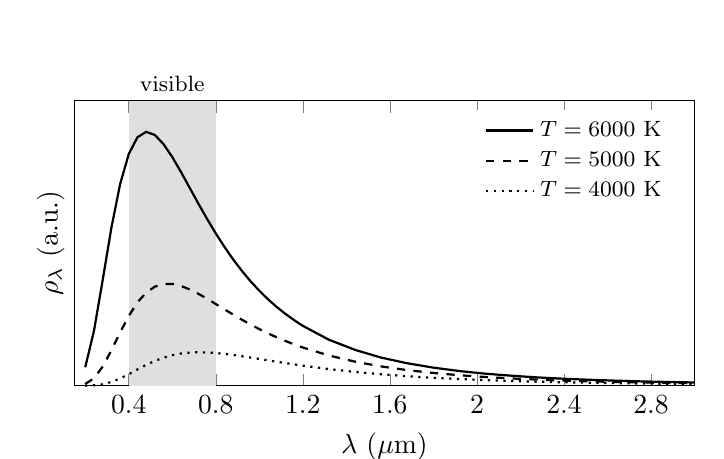
\begin{tikzpicture}
    \begin{axis}[width=0.78\textwidth, height=5.2cm,
      xlabel={$\lambda$ ($\mu$m)}, ylabel={$\rho_\lambda$ (a.u.)},
      xmin=0.15, xmax=3, ymin=0, ymax=0.30,
      ytick=\empty, xtick={0.4,0.8,1.2,1.6,2,2.4,2.8},
      legend pos=north east, legend cell align=left,
      legend style={draw=none, font=\footnotesize}, clip=false,
      every axis plot/.append style={thick}]
      \fill[gray!25] (axis cs:0.4,0) rectangle (axis cs:0.8,0.30);
      \node[font=\footnotesize, anchor=south] at (axis cs:0.6,0.30) {visible};
      \addplot[black] coordinates {(0.200,0.0194) (0.240,0.0575) (0.280,0.1109)
        (0.320,0.1660) (0.360,0.2119) (0.400,0.2439) (0.440,0.2616)
        (0.480,0.2673) (0.520,0.2640) (0.560,0.2543) (0.600,0.2408)
        (0.640,0.2250) (0.680,0.2084) (0.720,0.1917) (0.760,0.1756)
        (0.800,0.1603) (0.840,0.1461) (0.880,0.1329) (0.920,0.1209)
        (0.960,0.1099) (1.000,0.1000) (1.040,0.0910) (1.080,0.0829)
        (1.120,0.0756) (1.160,0.0690) (1.200,0.0630) (1.320,0.0484)
        (1.440,0.0377) (1.560,0.0296) (1.680,0.0236) (1.800,0.0190)
        (1.920,0.0154) (2.040,0.0126) (2.160,0.0105) (2.280,0.0087)
        (2.400,0.0073) (2.520,0.0062) (2.640,0.0053) (2.760,0.0045)
        (2.880,0.0039) (3.000,0.0034)};
      \addlegendentry{$T=6000$ K}
      \addplot[black, dashed] coordinates {(0.200,0.0018) (0.240,0.0078)
        (0.280,0.0200) (0.320,0.0371) (0.360,0.0559) (0.400,0.0734)
        (0.440,0.0877) (0.480,0.0980) (0.520,0.1043) (0.560,0.1071)
        (0.600,0.1071) (0.640,0.1050) (0.680,0.1014) (0.720,0.0968)
        (0.760,0.0915) (0.800,0.0860) (0.840,0.0804) (0.880,0.0749)
        (0.920,0.0695) (0.960,0.0644) (1.000,0.0596) (1.040,0.0551)
        (1.080,0.0509) (1.120,0.0471) (1.160,0.0435) (1.200,0.0402)
        (1.320,0.0318) (1.440,0.0253) (1.560,0.0203) (1.680,0.0164)
        (1.800,0.0134) (1.920,0.0110) (2.040,0.0091) (2.160,0.0076)
        (2.280,0.0064) (2.400,0.0054) (2.520,0.0046) (2.640,0.0039)
        (2.760,0.0034) (2.880,0.0029) (3.000,0.0026)};
      \addlegendentry{$T=5000$ K}
      \addplot[black, dotted] coordinates {(0.200,0.0000) (0.240,0.0004)
        (0.280,0.0015) (0.320,0.0039) (0.360,0.0076) (0.400,0.0121)
        (0.440,0.0171) (0.480,0.0219) (0.520,0.0261) (0.560,0.0295)
        (0.600,0.0321) (0.640,0.0339) (0.680,0.0349) (0.720,0.0352)
        (0.760,0.0350) (0.800,0.0344) (0.840,0.0335) (0.880,0.0323)
        (0.920,0.0310) (0.960,0.0296) (1.000,0.0282) (1.040,0.0267)
        (1.080,0.0252) (1.120,0.0238) (1.160,0.0224) (1.200,0.0211)
        (1.320,0.0175) (1.440,0.0145) (1.560,0.0120) (1.680,0.0100)
        (1.800,0.0083) (1.920,0.0070) (2.040,0.0059) (2.160,0.0050)
        (2.280,0.0042) (2.400,0.0036) (2.520,0.0031) (2.640,0.0027)
        (2.760,0.0023) (2.880,0.0020) (3.000,0.0018)};
      \addlegendentry{$T=4000$ K}
    \end{axis}
  \end{tikzpicture}
  \caption*{\footnotesize Densité spectrale de puissance d'une source thermique
  en fonction de la longueur d'onde pour différentes températures. The peak
  moves towards short longueurs d'onde as $T$ rises, and the spectrum is
  continuous and several hundred THz wide.}
\end{figure}

Une des principales caractéristiques du rayonnement thermique est d'être
complètement \emph{désordonné} : émission dans toutes les directions, sur un
spectre continu de fréquences, pas de relation de phase entre les différents
photons émis. En termes plus scientifiques, on dira que le rayonnement
thermique est \textbf{incohérent}. Ce type d'émission s'effectue sur un spectre
très large de plusieurs centaines de téra-Hertz (plusieurs micromètres en
longueur d'onde dans le vide), bien loin des caractéristiques des lasers et même
des diodes électroluminescentes. Ainsi le soleil émet non seulement un spectre
dans l'ensemble du visible mais également dans l'UV et l'IR.

\begin{example}[Everyday thermal sources]
  Dans notre quotidien, les sources de lumière sont en général produites par un
  rayonnement thermique. L'exemple le plus évident est le soleil mais l'ampoule
  à incandescence, le métal chauffé, le métal en fusion et même un corps humain
  émettent ce type de lumière (la longueur d'onde d'émission d'un corps humain
  étant autour de $10\ \mu$m) --- the emission a thermal camera records.
\end{example}

\begin{remark}[Thermodynamic equilibrium]
  À l'équilibre thermodynamique, état atteint par le système si on le laisse
  évoluer suffisamment longtemps sans apport d'énergie provenant de
  l'extérieur, les niveaux d'énergie ont une occupation moyenne qui décroit avec
  la valeur de l'énergie et ce d'autant plus rapidement que la température est
  basse. Lorsqu'il part d'un état initial hors équilibre contenant donc des
  constituants excités (atomes, molécules, …), le système va évoluer en
  permettant aux constituants de perdre leur énergie excédentaire, énergie qui
  sera soit évacuée par rayonnement d'onde électromagnétique, soit conservée
  dans le système sous forme de chaleur contribuant à fixer la température
  finale du système.
\end{remark}

\subsection{Les transitions radiatives : la luminescence}
Il existe d'autres manières d'émettre de la lumière. Ainsi, la lumière émise par
luminescence résulte de transitions atomiques entre deux états d'énergie
\emph{discrets} d'un atome ou d'une molécule. Ces transitions génèrent un
échange d'énergie $E_b-E_a$ qui peut s'effectuer de deux manières : dans la
plupart des cas de manière \textbf{non radiative}, sans émission ni absorption
de lumière, libérant alors dans le matériau de l'énergie cinétique sous forme de
\textbf{phonon} (quantum d'énergie de vibration du cristal) ; dans certains cas,
la transition est \textbf{radiative} et s'accompagne de l'absorption ou de la
génération d'un photon. C'est ce cas qui naturellement nous intéresse.

Considérons un système atomique à deux niveaux d'énergie $E_a$ et $E_b$. Les
atomes présents dans le matériau se trouvent dans l'un ou l'autre de ces états.
Nous appellerons $N_a$ la \textbf{population} du niveau $E_a$ qui sera considéré
comme niveau fondamental du système (nombre d'atomes par unité de volume dans
l'état $E_a$) et $N_b$ la population du niveau $E_b$. Entre ces niveaux sont
possibles des transitions radiatives correspondant à des photons de fréquences
$\nu_{ab}=(E_b-E_a)/h$. En 1917, Einstein montre qu'il existe trois types de
transitions entre niveaux d'énergie atomiques : l'\textbf{émission spontanée}
(\textit{spontaneous emission}), que l'on retrouve dans le cas des diodes
électroluminescentes, et les \textbf{transitions induites} (\textit{induced
transitions}) parmi lesquelles on distingue l'absorption stimulée et l'émission
stimulée, utilisée dans les lasers mais également dans les amplificateurs de
lumière.

\begin{figure}[h!]
  \centering
  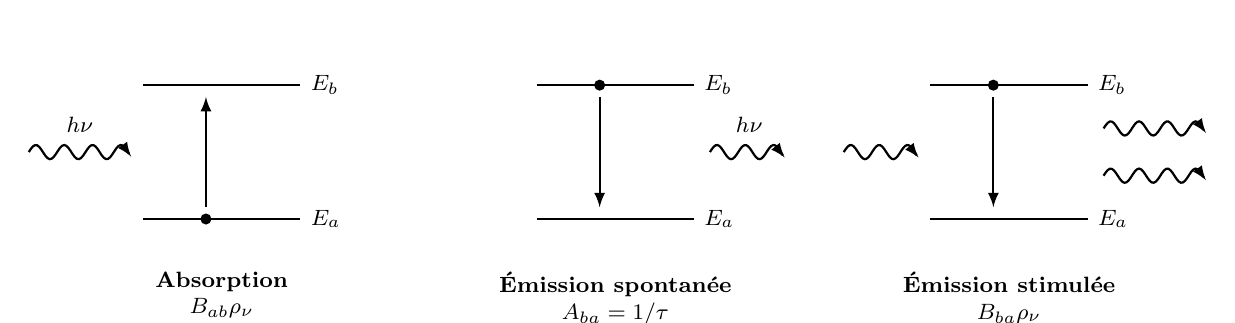
\begin{tikzpicture}[>=latex, every node/.style={font=\footnotesize}]
    \foreach \x in {0,5,10}{
      \draw[thick] (\x,0) -- (\x+2,0) node[right] {$E_a$};
      \draw[thick] (\x,1.7) -- (\x+2,1.7) node[right] {$E_b$};
    }
    % absorption
    \fill (0.8,0) circle (2pt);
    \draw[->, thick] (0.8,0.15) -- (0.8,1.55);
    \draw[->, thick] plot[domain=0:1.3, samples=50]
      ({-1.45+\x},{0.85+0.09*sin(\x*1000)});
    \node[anchor=south] at (-0.8,0.98) {$h\nu$};
    \node[anchor=north, align=center] at (1,-0.55)
      {\textbf{Absorption}\\$B_{ab}\rho_\nu$};
    % spontaneous
    \fill (5.8,1.7) circle (2pt);
    \draw[->, thick] (5.8,1.55) -- (5.8,0.15);
    \draw[->, thick] plot[domain=0:0.95, samples=40]
      ({7.2+\x},{0.85+0.09*sin(\x*1000)});
    \node[anchor=south] at (7.7,0.98) {$h\nu$};
    \node[anchor=north, align=center] at (6,-0.55)
      {\textbf{Émission spontanée}\\$A_{ba}=1/\tau$};
    % stimulated
    \fill (10.8,1.7) circle (2pt);
    \draw[->, thick] (10.8,1.55) -- (10.8,0.15);
    \draw[->, thick] plot[domain=0:0.95, samples=40]
      ({8.9+\x},{0.85+0.09*sin(\x*1000)});
    \draw[->, thick] plot[domain=0:1.3, samples=50]
      ({12.2+\x},{1.15+0.09*sin(\x*1000)});
    \draw[->, thick] plot[domain=0:1.3, samples=50]
      ({12.2+\x},{0.55+0.09*sin(\x*1000)});
    \node[anchor=north, align=center] at (11,-0.55)
      {\textbf{Émission stimulée}\\$B_{ba}\rho_\nu$};
  \end{tikzpicture}
  \caption*{\footnotesize The three Einstein transitions between two levels,
  with $h\nu=E_b-E_a$ throughout. The stimulated photon is a clone of the
  incident one.}
\end{figure}

\subsubsection{Transitions spontanées}
Seul l'état fondamental est stable dans un atome. Donc, après un certain temps,
l'atome excité finit par « retomber » spontanément à l'état fondamental en
émettant un photon d'énergie $h\nu_{ab}=E_b-E_a$, comme une bille, posée sur le
bord d'une baignoire, finirait, au moindre bruit ambiant, par retomber au fond
de cette dernière, spontanément.

\begin{definition}[Émission spontanée]
  Les émissions spontanées de photons par un ensemble d'atomes n'ont
  \emph{aucune corrélation} entre elles. Ces photons sont donc émis dans toutes
  les directions et n'ont pas de relation de phase entre eux tout comme le cas
  du rayonnement thermique : ils ne sont pas cohérents. Einstein note $A_{ba}$
  la probabilité (par atome et unité de temps) de ce phénomène.
\end{definition}

Contrairement au rayonnement thermique, l'énergie du photon spontané est
\emph{quantifiée}, le spectre est donc un spectre de raies. Cependant,
l'émission spontanée est fortement influencée par l'agitation thermique mais
aussi par des collisions entre atomes et/ou l'effet Doppler. Le spectre présente
donc en général l'aspect d'un continuum ou quasi-continuum s'étalant sur
plusieurs nanomètres. The hierarchy to remember is
\[\Delta\lambda_{\text{thermal}}\;\gg\;\Delta\lambda_{\text{spontaneous}}\;\gg\;
  \Delta\lambda_{\text{laser}},\qquad
  >\!\text{a few }\mu\text{m}\;\gg\;\text{a few nm}\;\gg\;
  \text{pm to }0.01\ \text{fm}.\]

\begin{conclusion}
  L'émission spontanée, appelée également luminescence, est un rayonnement
  \emph{incohérent} émis dans toutes les directions, avec un spectre beaucoup
  plus large que celui d'un laser mais moins que le rayonnement thermique.
\end{conclusion}

Cette luminescence peut être obtenue de plusieurs manières qui dépendent bien
souvent de la façon dont on va exciter le matériau. Cette excitation est
appelée \textbf{pompage} (\textit{pumping}).

\begin{itemize}
  \item La \textbf{photoluminescence} (excitation par absorption de photons),
    par exemple dans les tubes luminescents, les colorants fluorescents, les
    azurants optiques (un agent azurant est une molécule qui absorbe les
    rayonnements électromagnétiques ultraviolets entre 300 et 400 nm de
    longueur d'onde et réémet ensuite cette énergie par fluorescence dans le
    visible entre 400 et 500 nm). Parmi les phénomènes de photoluminescence, on
    distingue d'une part la \textit{fluorescence}, photoluminescence rapide (de
    $10^{-9}$ à $10^{-6}$ secondes pour la majorité des molécules organiques) et
    d'autre part la \textit{phosphorescence}, photoluminescence lente (de
    $10^{-3}$ à $10$ secondes). La chlorophylle absorbe le rouge et nous paraît
    donc verte.
  \item La \textbf{bioluminescence} (réaction enzymatique), utilisée par les
    lucioles.
  \item La \textbf{chimiluminescence} (excitation à la suite d'une réaction
    chimique), utilisée par exemple dans les bâtons lumineux ou le luminol.
    Durant une réaction de chimiluminescence, la molécule produite par la
    réaction se trouve dans un état excité. C'est le retour à l'état fondamental
    qui provoque le phénomène par l'émission d'une onde électromagnétique.
  \item L'\textbf{électroluminescence} (excitation électrique (champ
    électrique)), utilisée dans les diodes électroluminescentes (DEL), les
    télévisions.
\end{itemize}

\paragraph{Durée de vie d'un état excité}
Une particule excitée dans l'état $E_b$ peut spontanément passer dans l'état
$E_a$ par émission spontanée. Étudions l'évolution de la population sachant
qu'à l'instant $t=0$, on a grâce à l'excitation, une population $N_b^0$ plus
grande que la population à l'équilibre thermique (prise égale à 0). Durant
l'intervalle de temps $dt$, la population diminue de la quantité :
\[dN_b=-A_{ba}N_b\,dt=-N_b\frac{dt}{\tau}.\]
C'est la loi la plus simple que l'on puisse écrire, la perte est directement
proportionnelle à la population présente et à l'intervalle de temps étudié. La
constante $A_{ba}=1/\tau$ est le \textbf{premier coefficient d'Einstein}
(\textit{first Einstein coefficient}). En intégrant cette relation, on trouve :
\[\boxed{\,N_b=N_b^0\,e^{-t/\tau}\,}\]

\begin{definition}[Durée de vie (\textit{lifetime})]
  La constante $\tau$ est la durée de vie moyenne des états excités, c'est une
  caractéristique essentielle de chaque transition. La constante $A_{ba}$ varie
  en fonction du matériau étudié mais également suivant la transition
  considérée au sein d'un même matériau. En fait cette durée de vie rend compte
  de la capacité du matériau à faire varier ses populations par exemple en
  fonction d'une perturbation extérieure.
\end{definition}

The range of $\tau$ decides what a component is good for:
\begin{itemize}
  \item la dizaine de millisecondes pour certaines terres rares (ions Erbium
    dans une matrice de silice), permettant de faire des amplificateurs
    \emph{insensibles au débit}, c'est-à-dire avec une amplification qui ne
    varie pas entre deux bits d'information différents à des fréquences
    supérieures au GHz ;
  \item des temps inférieurs à la nanoseconde comme dans les semi-conducteurs,
    permettant de faire des composants \emph{rapides}.
\end{itemize}

\paragraph{Propriété spectrale d'une émission spontanée}
Naturellement, la puissance optique émise est proportionnelle au nombre de
désexcitations depuis l'état $\ket{b}$ vers l'état $\ket{a}$ par seconde, qui
est égal au nombre de photons émis, c'est-à-dire $h\nu A_{ba}N_b(t)$. La
décroissance de la puissance dans le temps suit donc la même loi de
décroissance en $e^{-t/\tau}$. Le champ prend donc la forme :
\[E(t)=E_0\,e^{-\frac{t}{2\tau}}\,e^{-j\omega_0 t}\qquad\text{for }t\geq 0.\]
Si on regarde la répartition des fréquences de ce champ dans le domaine
spectral, cela revient à faire une transformée de Fourier, vue largement dans
le chapitre « Diffraction ». The emission spectrum of a material whose
excited-state population decays exponentially is \textbf{lorentzien}. La densité spectrale de puissance de l'émission spontanée
s'écrit donc :
\[S_E(\omega)=\left|\mathcal{TF}[E(t)]\right|^2=E(\omega)E^*(\omega)
  =\frac{E_0^2}{\left(1/2\tau\right)^2+\left(\omega-\omega_0\right)^2}.\]
C'est une lorentzienne centrée sur la fréquence $\nu_0=\omega_0/2\pi$; its half
width at half maximum is
\[\Delta\omega=2\pi\Delta\nu=\frac{1}{2\tau}.\]

\begin{remark}
  The value $1/2\tau$ is a half width, not the \emph{total} width at half
  maximum: $S_E$ falls to half its maximum at $\omega-\omega_0=\pm 1/2\tau$, so
  $1/2\tau$ is the half width at half maximum and the full width is $1/\tau$.
  Keep this convention, but remember the factor 2 whenever a full width is
  wanted.
\end{remark}

\paragraph{Largeur naturelle et facteur d'élargissement}
Un état d'énergie n'est pas aussi discret que l'on veut bien le sous-entendre,
il présente donc naturellement une certaine largeur $\Delta E$. On comprend
alors que l'atome puisse émettre ou absorber des fréquences plus grandes et plus
petites que $\nu_{ab}=(E_b-E_a)/h$ avec une certaine probabilité $g(\nu)$. Le
champ électrique émis peut donc s'écrire :
\[E(t)=\int E_0\,g(\nu)\,e^{2j\pi\nu t}\,d\nu=E_0\,e^{-At/2}\,e^{2j\pi\nu_0 t}.\]
Cette largeur est en réalité encore plus grande à cause des chocs entre
particules ou encore à cause de l'effet Doppler dans le cas des gaz par exemple.
$g(\nu)$ est alors encore plus large qu'initialement et $g(\nu)$ qualifie
finalement la largeur spectrale de l'émission. Détailler l'expression de
$g(\nu)$ et les mécanismes d'élargissement est hors du propos de ce cours. On
appellera \emph{$g(\nu)$ la largeur réelle de la source luminescente}; it will
reappear as the gain curve of an amplifying medium.

\subsubsection{Les sources superluminescentes : la LED et la source « blanche » à fibre dopée à l'Erbium}
Toutes les sources dont le mécanisme d'émission est spontané sont appelées de
manière générique des sources \textbf{superluminescentes} ou
\textbf{superfluorescentes}.

\paragraph{La diode électroluminescente}
La plus connue du grand public est la \textbf{diode électroluminescente}
(\textit{light-emitting diode}, LED). Le milieu émetteur choisi est alors du
semiconducteur dont on choisit les caractéristiques en fonction de la couleur
que l'on souhaite obtenir. La première LED à spectre infrarouge, émettant une
intensité lumineuse extrêmement faible, a été créée en 1962. La diode bleue a
été inventée en 1990, suivie par la mise au point d'une diode émettant une
couleur blanche, ouvrant la voie à de nouvelles applications majeures,
notamment dans le domaine de l'éclairage et des écrans de télévisions et
d'ordinateurs. Les premières LED blanches sont peu à peu apparues sur le marché
et sont maintenant de plus en plus puissantes (d'une centaine de lumen pour 1 W
de consommation électrique --- équivalent à une ampoule à filament de 20 W ---
à un millier de lumen pour une vingtaine de watts électriques, équivalent à une
ampoule à filament de 100 W).

Les spectres des diodes blanches peuvent être très différents suivant la
technique utilisée; there are two routes to white.
\begin{subpart}
  \item \textbf{Diodes bleues + phosphore} : a blue LED is coated with phosphor
    granules which re-emit in the yellow; the sum of the blue luminescence and
    the yellow phosphorescence reads as white. Possibilité de plusieurs couches
    de différents phosphores pour élargir le spectre ; la plupart des LED
    blanches haute puissance fonctionnent sur ce principe. The colour
    temperature is tuned from blanc chaud (2670--3500 K) through blanc neutre
    (3500--4500 K) to blanc froid (4500--10\,000 K).
  \item \textbf{Diodes RVB} : génération de lumière blanche à l'aide de trois
    sources LED rouge, verte, bleue, typically at 465 nm, 532 nm and 630 nm.
    Coloris sans limite et ajustables, but assemblage complexe, difficile de
    faire de la haute puissance, and synthèse de certaines couleurs impossible
    --- kaki, marron, rose saturé, violet profond, turquoise profond.
\end{subpart}

Les LEDs ont une durée de vie (20\,000 à 50\,000 heures environ) beaucoup plus
longue qu'une lampe à incandescence classique (1000 heures) ou qu'une lampe
halogène (2000 heures), mais du même ordre de grandeur que les lampes
fluorescentes (5000 à 70\,000 heures). Les lampes à LED ont généralement une
efficacité énergétique nettement supérieure aux lampes classiques : 70 lumen/W
pour les fluocompactes et seulement 16 lumen/W pour les lampes à incandescence.

\paragraph{La source blanche à fibre dopée à l'Erbium}
Une autre source superluminescente est très utilisée dans le domaine des
télécoms, c'est la source à fibre dopée à l'Erbium. Son spectre d'émission,
semblable à la courbe de gain $g(\nu)$ introduite plus haut, s'étale de 1525 à
1565 nm, gamme de longueur d'onde dans l'infrarouge qui est la \textbf{bande C}
des télécoms. Its bande passante is $c\,\Delta\lambda/\lambda_0^2\approx 5$ THz.
Par abus de langage, on parle de source blanche car le spectre est large
comparé à celui du laser et parce qu'il couvre toute la bande C, de même que le
blanc couvre tout le visible.

\subsubsection{Transitions induites : absorption et émission}
Jusqu'à présent, nous avons mis au niveau supérieur des charges et étudié ce qui
se passe lorsqu'on laisse spontanément se désexciter l'atome. Cependant, si
avant ce phénomène, les atomes sont soumis à un rayonnement électromagnétique,
deux autres phénomènes peuvent avoir lieu : l'absorption et l'émission induite.

\begin{definition}[Absorption]
  On peut faire passer un atome de l'état fondamental d'énergie $E_a$ à l'état
  excité $E_b$ si on lui fournit l'énergie $E_b-E_a$. Cet apport d'énergie peut
  être fourni de plusieurs manières. Notamment, il peut se faire par
  l'absorption d'un photon incident d'énergie $h\nu$ suffisante. La probabilité
  correspondante sera notée $B_{ab}\rho_\nu$ où $\rho_\nu$ est la densité
  spectrale énergétique (énergie par unité de volume et unité de fréquence) du
  rayonnement incident. Ainsi, si $N_a$ est le nombre d'atomes (appelé
  « population ») dans l'état fondamental $\ket{a}$, le nombre $dN'_b$ de ces
  atomes qui vont passer dans l'état excité $\ket{b}$ est à la fois
  proportionnel à la population $N_a$, à la durée d'observation $dt$ et enfin à
  la densité spectrale d'énergie $\rho_\nu$ :
  \[dN'_b=+B_{ab}\,\rho_\nu\,N_a\,dt.\]
  $B_{ab}$ is the \textbf{deuxième coefficient d'Einstein} (\textit{second
  Einstein coefficient}).
\end{definition}

\begin{definition}[Émission stimulée]
  En 1917, Einstein imagina que si un photon traverse le milieu avec une énergie
  suffisante, il peut provoquer la désexcitation d'un atome qui libère alors son
  énergie de transition sous forme d'un photon : l'atome peut donc revenir à
  l'état fondamental de façon \emph{stimulée}. C'est la transition inverse de
  l'absorption :
  \[dN''_b=-B_{ba}\,\rho_\nu\,N_b\,dt,\]
  with $B_{ba}$ the \textbf{troisième coefficient d'Einstein} (\textit{third
  Einstein coefficient}).
\end{definition}

Comme la bille sur le bord de la baignoire à qui on mettrait une petite
pichenette pour la faire redescendre, sans attendre qu'elle ne redescende
spontanément. The essential point is the nature of the emitted photon.

\begin{postulate}[Clone du photon incident]
  Le photon émis possède la \emph{même phase}, la \emph{même fréquence}, la
  \emph{même polarisation} ainsi que la \emph{même direction} que le photon
  incident. Le rayonnement incident est donc amplifié. On peut même dire que les
  photons sont clonés. L'onde EM émise par émission stimulée est donc
  \textbf{cohérente}.
\end{postulate}

\begin{remark}
  Contrairement au cas de l'émission spontanée, il existe un champ excitateur
  (ici un champ électromagnétique déjà formé, transportant de l'énergie)
  caractérisé par une phase, une polarisation, une direction de propagation et
  une fréquence bien définie. L'atome va donc être désexcité sous l'action de ce
  champ bien défini et le champ émis aura les mêmes caractéristiques.
\end{remark}

\paragraph{Les équations d'Einstein}
Il existe des relations entre les coefficients d'Einstein. Pour le voir, on
considère un champ thermique dans lequel baignent des molécules dont $N_a$ se
trouvent dans l'état $\ket{a}$ et $N_b$ dans l'état $\ket{b}$. On considère que
le système se trouve dans un état stationnaire, ce qui fait qu'il y a autant de
transitions de l'état $\ket{a}$ vers $\ket{b}$ que de $\ket{b}$ vers $\ket{a}$.
Ceci découle de la stationnarité du nombre de photons dans le mode, et
s'exprime par :
\[\text{spontaneous emission}+\text{stimulated emission}=\text{absorption},\]
that is, collecting the three rate equations,
\[N_b\left(A_{ba}+B_{ba}\rho_\nu\right)=N_a B_{ab}\rho_\nu
  \quad\Longrightarrow\quad
  \rho_\nu=\frac{N_bA_{ba}}{N_aB_{ab}-N_bB_{ba}}
  =\frac{A_{ba}}{B_{ab}\dfrac{N_a}{N_b}-B_{ba}}.\]
Si on considère que la probabilité d'occupation d'un état excité d'énergie $E$
dans le cas stationnaire est donnée par la statistique de Maxwell--Boltzmann,
$N_n\propto e^{-E_n/k_BT}$, les rapports de populations prennent la forme :
\[\frac{N_a}{N_b}=\frac{e^{-E_a/k_BT}}{e^{-E_b/k_BT}}
  =e^{\frac{E_b-E_a}{k_BT}}=e^{\frac{h\nu}{k_BT}}.\]
Si $E_b>E_a$, \emph{naturellement} $N_b<N_a$. Substituting this ratio and the
loi de Planck into the expression for $\rho_\nu$ gives
\[e^{h\nu/k_BT}\left[\frac{8\pi h\nu^3}{c^3}B_{ab}-A_{ba}\right]
  =\left[\frac{8\pi h\nu^3}{c^3}B_{ba}-A_{ba}\right].\]

\begin{theorem}[Égalité des coefficients induits]
  Cette équation doit être vérifiée quelle que soit la température. Donc, les
  deux membres doivent être séparément nuls, ce qui donne
  \[\boxed{\,B_{ab}=B_{ba}\,}\]
  La probabilité d'émission stimulée est égale à la probabilité d'absorption.
\end{theorem}

\paragraph{L'amplification optique : nécessité d'un pompage}
Ceci a une incidence sur la capacité d'un milieu à amplifier de la lumière. En
effet, à l'équilibre thermique, la population du niveau haut est inférieure à
la population du niveau bas. Puisque $B_{ab}=B_{ba}$, \emph{naturellement, un
milieu absorbe plus qu'il n'amplifie}.

\begin{center}
  \begin{tabular}{lcccc}
    \toprule
    & $\nu$ (Hz) & $h\nu$ (\eV) & $h\nu/k_BT$ & $N_b/N_a$ \\
    \midrule
    100 nm (UV)        & $3\cdot10^{15}$ & $12.38$            & $495$   & $10^{-215}$ \\
    500 nm (visible)   & $6\cdot10^{14}$ & $2.48$             & $96$    & $10^{-42}$ \\
    10 $\mu$m (IR)     & $3\cdot10^{13}$ & $0.12$             & $4.95$  & $0.01$ \\
    1 mm (Hertzien)    & $3\cdot10^{11}$ & $1.24\cdot10^{-3}$ & $0.05$  & $0.95$ \\
    \bottomrule
  \end{tabular}
\end{center}

\noindent À température ambiante, à l'équilibre. Le mot « clé » dans l'étude
des lasers est l'\textbf{inversion de population} (\textit{population
inversion}), c'est-à-dire faire en sorte que $N_b>N_a$. On comprend après
examen de ce tableau que cette inversion de population ait pu se faire plus
facilement dans le domaine hertzien (MASER, inventé en 1953 à l'université
Columbia par Charles Townes, James Gordon et Herbert Zeiger --- le maser à
ammoniac) que dans le domaine visible, where the table gives $10^{-42}$. The
more reasonable ratio in the infrared is the course's explanation for the first
lasers, in 1960, operating at 0.85 $\mu$m. At the other extreme, très difficile
de réaliser un laser UV : pompage extrêmement fort. The laser excimer
(chirurgie oculaire) works because an excimer is a molécule stable \emph{à
l'état excité}.

\begin{remark}
  Two rows worked through. At 500 nm the photon energy is $h\nu=2.48\ \eV$, so
  $h\nu/k_BT\approx 96$ and $N_b/N_a\approx 10^{-42}$; on the 1 mm row
  $h\nu/k_BT$ is only $0.05$, which is what gives $N_b/N_a=0.95$. Inversion is
  easy in the Hertzian domain and hopeless in the UV.
\end{remark}

On peut représenter l'évolution de l'intensité d'une onde qui traverse un milieu
par l'expression :
\[I(z)=I(0)\,e^{-\alpha z},\qquad \alpha=a\left(N_a-N_b\right),\]
où $\alpha$ est le coefficient d'atténuation linéique (en m$^{-1}$),
naturellement positif. Pour que $\alpha$ change de signe et devienne un
coefficient d'amplification, il faut que $N_b>N_a$ : c'est ce qu'on appelle une
inversion de population.

\begin{remark}
  The coefficient $\alpha=a(N_a-N_b)$ does not depend on the intensity: it is a
  coefficient in m$^{-1}$ and appears inside the exponential.
\end{remark}

\paragraph{Inversion de population par pompage}
Pour rompre avec la distribution caractéristique de l'équilibre thermique et
rendre un milieu amplificateur, a pompage is needed. Ce pompage est réalisé en
utilisant une source d'énergie extérieure. Il existe différents types de
pompage suivant le matériau considéré. En voici une liste non exhaustive :

\begin{itemize}
  \item Le \textbf{pompage optique} (\textit{optical pumping}) : on peut faire
    passer des électrons d'un niveau fondamental vers un niveau excité par
    absorption d'un champ électromagnétique. On montre que pour que ce pompage
    permette d'atteindre l'inversion de population, le modèle à deux niveaux
    d'énergie \emph{n'est pas} suffisant. Il faut alors recourir à des systèmes
    à 3 voire 4 niveaux d'énergie. C'est le cas du laser solide Nd:YAG, des
    lasers et amplificateurs à fibres dopées aux terres rares.
  \item Le \textbf{pompage électrique} (\textit{electrical pumping}) : dans un
    laser à semiconducteur, le passage d'un courant direct dans une jonction PN
    provoque dans une même région l'apparition d'électrons dans un état excité
    (bande de conduction) et simultanément de places vides d'électrons (trous)
    dans des états de moindre énergie (la bande de valence). La recombinaison de
    ces paires électron--trou permet l'émission de lumière. On retrouve ce
    procédé aussi bien dans les LED que les amplificateurs ou lasers à
    semiconducteur.
  \item Le \textbf{pompage collisionnel} (\textit{collisional pumping}) : une
    décharge électrique dans un gaz entraîne des collisions entre électrons et
    atomes (ou ions ou molécules) qui peuvent entrainer une inversion de
    population. Par exemple, dans le laser He--Ne, la décharge électrique excite
    essentiellement l'Hélium (5 à 6 fois plus important que le Néon) sur un
    état métastable (à longue durée de vie) qui se désexcite par collision
    résonnante sur le Néon qui, lui, réémet de manière radiative autour de
    633 nm.
  \item Le \textbf{pompage chimique, photochimique} : réaction chimique (pas
    forcément initiée par de la lumière) dont les produits se forment dans un
    état excité. Par exemple : $\mathrm{H_2+F_2\to 2HF}$. Les molécules de HF
    sont excitées à l'arrivée.
\end{itemize}

\subsubsection{L'amplificateur optique}
Avant d'utiliser ce milieu amplificateur pour réaliser des lasers, on peut
d'abord utiliser ce milieu pour amplifier la lumière. D'une manière générale, le
signal que l'on souhaite amplifier est injecté dans l'amplificateur
(généralement composé d'un guide optique). Ce signal va être amplifié par
émission stimulée tout au long de sa propagation à chaque fois que les photons
rencontreront des atomes excités préalablement par un pompage. L'amplification
réside donc dans une \emph{cascade de clonage} du photon incident au fur et à
mesure de sa propagation dans l'amplificateur.

Cependant, tous les atomes excités ne se désexciteront pas de manière stimulée.
Simultanément à l'amplification désirée du signal incident, certains atomes se
désexciteront de manière spontanée. Ce rayonnement n'est pas cohérent avec le
signal amplifié. En d'autres termes, l'amplificateur optique émet \emph{un
bruit}, comme un amplificateur électronique, qui s'ajoute au signal à amplifier,
dégradant par la même occasion le rapport signal à bruit. Cette émission
spontanée est émise à tout endroit dans le guide et potentiellement dans toutes
les directions. Chaque photon émis spontanément dans le cône d'acceptance du
guide et dans la bonne direction traverse un milieu amplificateur et va donc
également être amplifié en se propageant vers la sortie par émission stimulée.

\begin{definition}[ASE]
  En sortie du guide, on observe donc de l'\textbf{émission spontanée amplifiée}
  (\textit{amplified spontaneous emission}, ASE) qui s'ajoute au signal incident
  amplifié $P_1=G\,P_0$ --- a broadband noise floor. Naturellement, ce rapport
  entre émission spontanée et émission stimulée varie en fonction de la
  puissance d'entrée. Le gain \emph{et} le rapport signal à bruit d'un ampli
  sont donc dépendants de la puissance d'entrée.
\end{definition}

\begin{remark}[Communicating vessels]
  Émission stimulée and émission spontanée draw on the same excited population:
  if $E_{\text{stimulated}}$ increases, $E_{\text{spontaneous}}$ decreases. Pour
  limiter le bruit ASE, il faut \emph{rapprocher} les amplis les uns des autres,
  so that each sees a larger input power.
\end{remark}

\paragraph{L'amplificateur Erbium}
Depuis l'apparition des fibres monomodes dans les années 80 dans les systèmes
optiques de communication, l'atténuation est un facteur à combattre pour
allonger la portée des liaisons inter-urbaines ou sous-marines. L'apparition de
l'amplificateur à fibre dopée à l'Erbium (EDFA) en 1987 et qui a été déployé au
début des années 90 a permis de s'affranchir de la régénération complexe
opto-électronique. Le signal est amplifié en traversant un tronçon de fibre
dopée, directement connectée à la fibre de transmission. Amplification
\emph{en ligne} : pas de conversion opto-électronique.

\begin{figure}[h!]
  \centering
  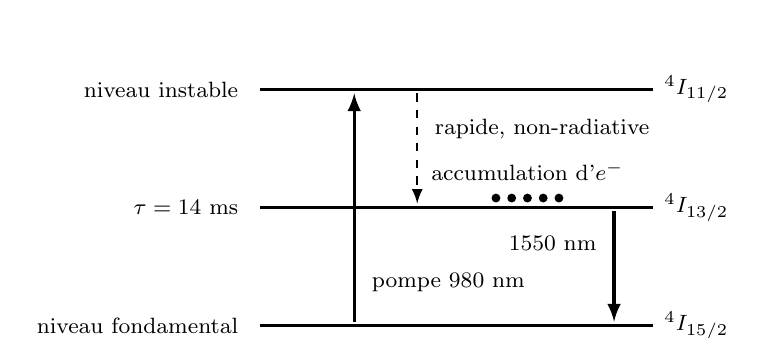
\begin{tikzpicture}[>=latex, every node/.style={font=\footnotesize}]
    % levels
    \draw[very thick] (0,0) -- (5,0) node[right] {$^4I_{15/2}$};
    \draw[very thick] (0,1.5) -- (5,1.5) node[right] {$^4I_{13/2}$};
    \draw[very thick] (0,3.0) -- (5,3.0) node[right] {$^4I_{11/2}$};
    \node[anchor=east, align=right] at (-0.15,3.0) {niveau instable};
    \node[anchor=east, align=right] at (-0.15,1.5) {$\tau=14$ ms};
    \node[anchor=east, align=right] at (-0.15,0) {niveau fondamental};
    % pump
    \draw[->, very thick] (1.2,0.05) -- (1.2,2.95);
    \node[anchor=west] at (1.3,0.55) {pompe 980 nm};
    % non-radiative
    \draw[->, thick, dashed] (2.0,2.95) -- (2.0,1.55);
    \node[anchor=west] at (2.1,2.5) {rapide, non-radiative};
    % lasing
    \draw[->, very thick] (4.5,1.45) -- (4.5,0.05);
    \node[anchor=east] at (4.4,1.05) {1550 nm};
    % accumulation dots
    \foreach \x in {3.0,3.2,...,3.8}{\fill (\x,1.62) circle (1.6pt);}
    \node[anchor=south] at (3.4,1.72) {accumulation d'$e^-$};
  \end{tikzpicture}
  \caption*{\footnotesize Système à 3 niveaux d'un amplificateur à fibre dopée
  erbium. The long durée de vie of $^4I_{13/2}$ is what gives the EDFA its
  transparence au débit.}
\end{figure}

\noindent On peut effectuer du pompage dans les différentes bandes
d'absorption de l'Erbium --- autour de 800 nm, autour de 980 nm et autour de
1480 nm. En pratique, on utilise l'absorption d'une onde à 980 nm fournie par
une diode laser puissante pour réaliser le pompage et l'émission radiative
s'effectue entre 1525 nm et 1565 nm. Une fibre dopée Erbium peut être
approximée par un système à trois niveaux. La transition
$^4I_{15/2}\to{}^4I_{11/2}$ permet d'absorber l'énergie d'une onde pompe à
980 nm. Les atomes sont donc transférés du niveau fondamental vers le niveau
excité. La transition $^4I_{11/2}\to{}^4I_{13/2}$ est très rapide et
non-radiative. Les atomes sont donc quasi-instantanément transférés vers le
niveau $^4I_{13/2}$ qui a une durée de vie très longue de 14 ms. Toutes les
conditions sont ainsi remplies pour obtenir une inversion de population entre
les niveaux $^4I_{13/2}$ et $^4I_{15/2}$ et donc une transition laser radiative
autour de 1550 nm permettant l'amplification à ces longueurs d'onde par
émission stimulée. Pour un gain suffisant, la fibre mesure une dizaine de
mètres et est lovée sur une bobine de 5 à 10 cm de diamètre.

\begin{conclusion}[Why the EDFA revolutionised optical telecommunications]
  Ce qui est intéressant pour les communications haut débit est la durée de vie
  de l'état $^4I_{13/2}$, très longue ($\tau=14$ ms), which corresponds to a
  bande passante $1/\tau\approx 70$ Hz. Cela rend cet amplificateur très peu
  réactif aux variations très rapides de la puissance d'entrée à amplifier,
  puisque cette constante de temps est directement reliée à la vitesse à
  laquelle est capable de varier la population de cet état --- and hence the
  gain. Ainsi, par exemple à 10 Gb/s, le gain de l'amplification est le même
  quelle que soit la valeur du bit d'entrée (0 ou 1). Le taux d'extinction
  $I_1/I_0$ n'est donc pas modifié aux hautes fréquences avec ce type
  d'amplificateur (hormis l'ajout d'un bruit) : on parle de
  \textbf{transparence au débit} (\textit{transparency to the bit rate}).
  L'EDFA est donc utilisé sur des transmissions haut débit, directement soudé à
  la fibre de transmission, tous les 100 km pour une liaison terrestre et tous
  les 50 à 70 km pour les transmissions sous-marines.
\end{conclusion}

\paragraph{L'amplificateur à semiconducteur}
Le fonctionnement de ce type d'amplificateur se modélise par un système à deux
niveaux associé à un pompage électronique. D'une manière générale, ce qu'il
faut retenir est que la durée de vie des porteurs dans la bande de conduction
est \emph{beaucoup plus rapide} que pour l'Erbium. Elle est de l'ordre de la
nanoseconde ou du dixième de nanoseconde, so a bande passante of a few GHz. Les
populations peuvent donc varier entre les 1 et les 0 d'un signal à 10 Gb/s
entrainant une modification du gain rapide et donc des distorsions du signal
entrant. On dit que son fonctionnement est \emph{non-linéaire}. Ce type
d'amplificateur n'est donc pas (ou peu) utilisé pour les amplificateurs optiques
en ligne sur de longues distances. Par contre, il est utilisé pour réaliser des
fonctions optiques : commutation, traitement du signal, etc. et depuis peu pour
le réseau d'accès.

On the other hand its gain per unit length is several orders of magnitude above
erbium's, so un amplificateur à semiconducteur d'une longueur de quelques
millimètres permet d'avoir le même gain qu'un EDFA pour lequel la fibre doit
avoir une longueur d'une dizaine de mètres. L'amplificateur à semiconducteur est
donc bien plus intégrable qu'un EDFA; a packaged device is about 2 cm.

\subsection{Le laser : le milieu amplificateur plongé dans une cavité résonante}
Nous avons vu comment on pouvait obtenir un milieu amplificateur. Pour obtenir
un laser, il suffit de placer ce milieu amplificateur dans une cavité résonante
et de respecter certaines conditions. Le fait de faire aller et venir la lumière
dans le milieu amplificateur à l'aide d'une cavité optique permet d'augmenter
considérablement la capacité d'amplification d'une onde puisque celle-ci va
transiter plusieurs fois dans le milieu. Ce facteur d'amplification élevé peut
compenser la perte d'énergie due à l'émission d'énergie vers l'extérieur,
indispensable si l'on veut que de la lumière sorte du laser. Toutes sortes de
cavités : miroirs plan / plan (cavité Fabry--Perot), miroirs plan / concave, en
anneau, à fibre.

\subsubsection{La cavité résonante}
La façon la plus simple pour expliquer le principe de fonctionnement d'une
cavité résonante est de considérer la cavité Fabry--Perot constituée de deux
miroirs plans, face à face, avec $r_1,r_2$ les facteurs de réflexion en
amplitude de chaque miroir et $t_1,t_2$ les facteurs de transmission
correspondants. Dans ce type de cavité, les réflexions successives sur chaque
miroir vont engendrer des interférences entre un grand nombre d'ondes
cohérentes --- un problème d'interférences à ondes multiples.

\begin{prop}[Sélectivité spectrale (\textit{wavelength selectivity})]
  Si le déphasage accumulé sur un aller-retour est un multiple de $2\pi$, les
  ondes s'ajoutent en phase, le champ est alors transmis par la cavité. If the
  phase is offset by $\pi$, the ondes superpose in phase opposition, the field
  cancels and is no longer transmitted. Une telle cavité résonante est donc
  \emph{sélective en longueur d'onde} comme une corde de guitare.
\end{prop}

\noindent Si on note $\psi_0$ l'amplitude complexe d'une onde plane incidente
(with $e$ the cavity length, filled with index $n$), les amplitudes complexes
des ondes transmises après un nombre d'allers-retours successifs s'écrivent :
\[\psi_1=t_1t_2\psi_0e^{i\varphi/2},\quad
  \psi_2=r_1r_2t_1t_2\psi_0e^{i\varphi}e^{i\varphi/2},\quad
  \psi_3=r_1^2r_2^2t_1t_2\psi_0e^{i2\varphi}e^{i\varphi/2},\quad\ldots\]
où
\[\varphi=\frac{2\pi}{\lambda_0}\,2ne\]
désigne la différence de phase accumulée par une onde sur un aller-retour. Si on
introduit les facteurs de réflexion et de transmission en intensité de chacun
des miroirs, en prenant pour simplifier les calculs $r=r_1=r_2$ et $t=t_1=t_2$ :
$R=r^2$ et $T=t^2$. L'amplitude complexe de l'onde transmise au point $P$ du
plan focal de la lentille de collection est la somme des amplitudes complexes des ondes
transmises :
\[\psi_t(P)=\sum_i\psi_i
  =T\psi_0\left[1+Re^{i\varphi}+R^2e^{i2\varphi}+\cdots+R^me^{im\varphi}
  +\cdots\right]e^{i\varphi/2}.\]
C'est une suite géométrique de raison $Re^{i\varphi}$. Puisque $R<1$, on trouve
après sommation :
\[\psi_t(P)=T\psi_0\,\frac{1}{1-Re^{i\varphi}}\,e^{i\varphi/2},\]
et l'intensité de l'onde transmise résulte immédiatement de l'équation
précédente :
\[I_t(P)\propto\left|\psi_t(P)\right|^2
  =\frac{I_{max}}{1+M\sin^2\dfrac{\varphi}{2}},\qquad
  M=\frac{4R}{(1-R)^2},\qquad
  I_{max}=I_0\left(\frac{T}{1-R}\right)^2.\]

\begin{definition}[Fonction d'Airy]
  La fonction
  \[A(\varphi)=\frac{1}{1+M\sin^2\dfrac{\varphi}{2}}\]
  est appelée \textbf{fonction d'Airy} (\textit{Airy function}). C'est une
  fonction paire, symétrique. Chaque pic est appelé \textbf{mode longitudinal}
  (\textit{longitudinal mode}) de la cavité.
\end{definition}

Pour $\varphi$ petit devant $\pi$ (autour du pic centré autour de
$\varphi=0\ [2\pi]$), on peut écrire que :
\[A(\varphi)=\frac{1}{1+M\sin^2\left(\varphi/2\right)}
  \approx\frac{1}{1+M\left(\varphi/2\right)^2},\]
on reconnaît l'expression d'une lorentzienne : la fonction d'Airy est donc
constituée d'une succession de pics dont le profil est lorentzien.
L'interférence de ces ondes sera constructive et maximale si et seulement si $R$
est voisin de 1. Les très bons lasers possèdent des facteurs de réflexion en
amplitude des deux miroirs en valeur absolue proches de 1, les ondes véhiculées
par les différents rayons transmis ont alors pratiquement la même amplitude. Par
contre, les lasers à semiconducteur peuvent se permettre d'avoir des facteurs de
réflexion de l'ordre de 30\% seulement car le gain est très fort.

\begin{figure}[h!]
  \centering
  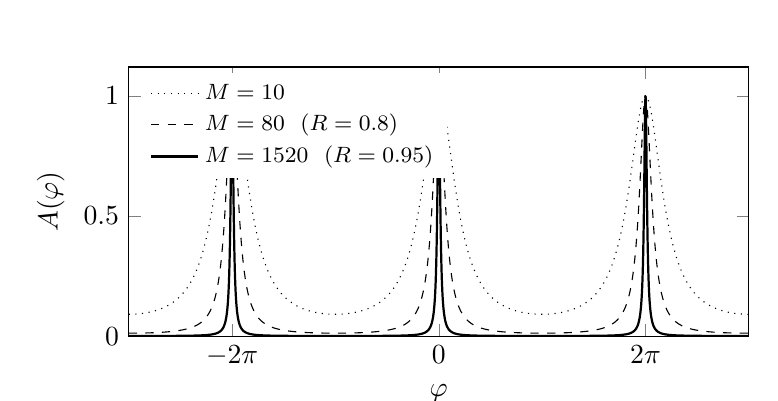
\begin{tikzpicture}
    \begin{axis}[width=0.78\textwidth, height=5cm,
      xlabel={$\varphi$}, ylabel={$A(\varphi)$},
      xmin=-1.5, xmax=1.5, ymin=0, ymax=1.12,
      xtick={-1,0,1}, xticklabels={$-2\pi$,$0$,$2\pi$},
      ytick={0,0.5,1},
      legend style={draw=none, font=\footnotesize, at={(0.02,0.98)},
        anchor=north west},
      legend cell align=left, samples=2400]
      \addplot[black, dotted, domain=-1.5:1.5] {1/(1+10*(sin(180*x))^2)};
      \addlegendentry{$M=10$}
      \addplot[black, dashed, domain=-1.5:1.5] {1/(1+80*(sin(180*x))^2)};
      \addlegendentry{$M=80$ \ ($R=0.8$)}
      \addplot[black, thick, domain=-1.5:1.5] {1/(1+1520*(sin(180*x))^2)};
      \addlegendentry{$M=1520$ \ ($R=0.95$)}
    \end{axis}
  \end{tikzpicture}
  \caption*{\footnotesize La fonction d'Airy est représentée pour trois valeurs
  de $M$. Plus $R$ augmente, plus les pics sont fins. Successive peaks are
  separated by the intervalle spectral libre $c/2ne$.}
\end{figure}

\paragraph{Largeur d'un mode}
On détermine la largeur totale à mi-hauteur en résolvant $A(\varphi)=0.5$ :
\[\Delta\varphi_{1/2}=\frac{4}{\sqrt{M}}=\frac{2(1-R)}{\sqrt{R}}.\]
Ainsi, plus $R$ augmente, plus la largeur des pics diminue. Application
numérique : pour $R=0.8$, $M=80$ et $\Delta\varphi_{1/2}\approx 0.45$ ; pour
$R=0.95$, $M=1520$ et $\Delta\varphi_{1/2}\approx 0.1$.

Rather than in phase, on peut convertir l'axe en longueur d'onde. Puisque
$\varphi_{AR}=2\pi\,2ne/\lambda_0$, alors
$\Delta\varphi=2\pi\,2ne\,\Delta\lambda/\lambda_0^2$, soit la largeur à
mi-hauteur exprimée en mètres :
\[\Delta\lambda_{1/2}=\frac{\lambda_0^2}{2\pi\,2ne}\,\Delta\varphi_{1/2}
  =\frac{\lambda_0^2}{2\pi\,2ne}\,\frac{2(1-R)}{\sqrt{R}}.\]

\begin{example}[Orders of magnitude]
  Si $\lambda_0=0.5\ \mu$m, $e=1$ cm et $n=1$ : pour $R=0.8$,
  $\Delta\lambda_{1/2}=0.89$ pm ; pour $R=0.95$, $0.2$ pm ; et pour $R=0.99$,
  $0.04$ pm. A Fabry--Perot cavity is an extraordinarily fine filter.
\end{example}

\begin{definition}[Intervalle spectral libre]
  L'espacement entre les pics de la fonction d'Airy, appelé
  \textbf{intervalle spectral libre} (\textit{free spectral range}), vaut
  \[\mathrm{ISL}=\frac{c}{2ne}.\]
\end{definition}

\begin{remark}[Confinement means quantisation]
  The mechanism is general: confining an onde quantises something. Corde
  vibrante : confinement longitudinal, quantification des fréquences (comme la
  cavité résonante optique). Fibre optique : confinement transverse,
  quantification de $k_x$ dans la direction de confinement (angles permis) ;
  il existe également un confinement angulaire. Électron dans un puits de
  potentiel : confinement autour de l'atome, quantification des énergies.
\end{remark}

\subsubsection{Le laser}
Le laser est constitué d'un milieu amplificateur inséré dans une cavité
résonante. Plaçons-nous dans le cas d'une cavité à miroirs plans parallèles
appelée cavité Fabry--Perot. Considérons une onde (provenant de l'émission
spontanée) qui prend naissance dans le milieu amplificateur. Au fur et à mesure
de sa propagation, elle va stimuler un certain nombre de transitions et s'en
trouver amplifiée. Si la direction est normale aux miroirs, l'onde émise est
renvoyée dans le milieu amplificateur où elle effectue un certain nombre
d'allers-retours entrecoupés de réflexions.

\begin{figure}[h!]
  \centering
  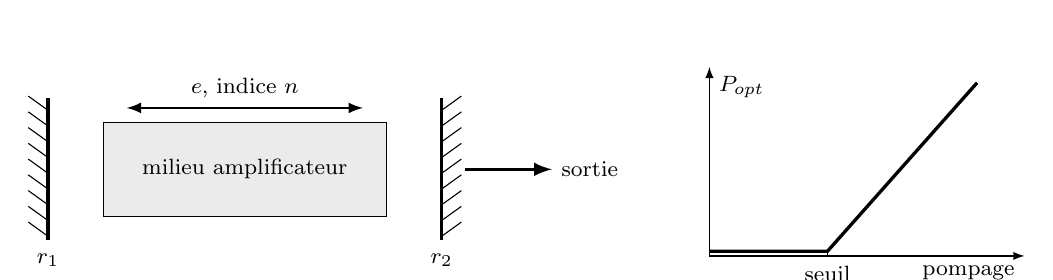
\begin{tikzpicture}[>=latex, every node/.style={font=\footnotesize}]
    % mirrors
    \draw[very thick] (0,-0.9) -- (0,0.9);
    \draw[very thick] (5,-0.9) -- (5,0.9);
    \foreach \y in {-0.85,-0.65,...,0.85}{
      \draw (0,\y) -- (-0.25,\y+0.18);
      \draw (5,\y) -- (5.25,\y+0.18);}
    \draw[fill=black!8] (0.7,-0.6) rectangle (4.3,0.6);
    \node at (2.5,0) {milieu amplificateur};
    \draw[<->, thick] (1.0,0.78) -- (4.0,0.78);
    \node[anchor=south] at (2.5,0.78) {$e$, indice $n$};
    \node[anchor=north] at (0,-0.95) {$r_1$};
    \node[anchor=north] at (5,-0.95) {$r_2$};
    \draw[->, very thick] (5.3,0) -- (6.4,0);
    \node[anchor=west] at (6.4,0) {sortie};
    % threshold curve
    \begin{scope}[xshift=8.4cm, yshift=-1.1cm]
      \draw[->] (0,0) -- (4.0,0) node[anchor=north east] {pompage};
      \draw[->] (0,0) -- (0,2.4) node[anchor=north west] {$P_{opt}$};
      \draw[very thick] (0,0.06) -- (1.5,0.06) -- (3.4,2.2);
      \draw[dashed] (1.5,0) -- (1.5,0.06);
      \node[anchor=north] at (1.5,0) {seuil};
    \end{scope}
  \end{tikzpicture}
  \caption*{\footnotesize Left: le milieu amplificateur plongé dans une cavité
  résonante. Right: existence d'un seuil --- below it the laser emits only
  émission spontanée amplifiée filtrée.}
\end{figure}

\begin{prop}[Les deux conditions d'oscillation]
  Pour que l'onde continue à croître, il faut que le gain compense les pertes
  dues aux réflexions et à l'absorption du milieu et des miroirs. Il faut
  également qu'après un aller-retour, l'onde revienne en phase avec elle-même :
  si elle est en phase, il va y avoir des interférences constructives et
  l'oscillation ainsi que l'amplification vont se poursuivre ; si elle n'est pas
  en phase, les interférences destructives vont rajouter des pertes qui feront
  que la condition de gain ne sera plus respectée. Hence the two
  \textbf{conditions de seuil d'oscillation} (\textit{oscillation threshold
  conditions}):
  \[\text{gain condition:}\quad
    \text{Gain}_{\text{round trip}}=\text{Losses}_{\text{round trip}},\qquad
    \text{phase condition:}\quad
    \varphi_{\text{round trip}}=2k\pi,\ k\in\zee.\]
\end{prop}

\begin{conclusion}
  La première, imposant un gain minimum, détermine l'\emph{inversion de
  population} nécessaire. La seconde, fixant la rotation de phase de l'onde
  oscillante lors d'un aller et retour, justifie l'introduction des \emph{modes}
  de la cavité, et impose la fréquence exacte d'oscillation.
\end{conclusion}

Lorsque la condition de gain est respectée, toute onde de fréquence proche de
celle du centre de la raie et cheminant parallèlement à l'axe de la cavité, voit
son amplitude accrue après une traversée et une réflexion et peut
potentiellement « laser ». Cependant, as the fonction d'Airy shows, toutes les
fréquences optiques ne peuvent pas osciller dans la cavité.

\begin{figure}[h!]
  \centering
  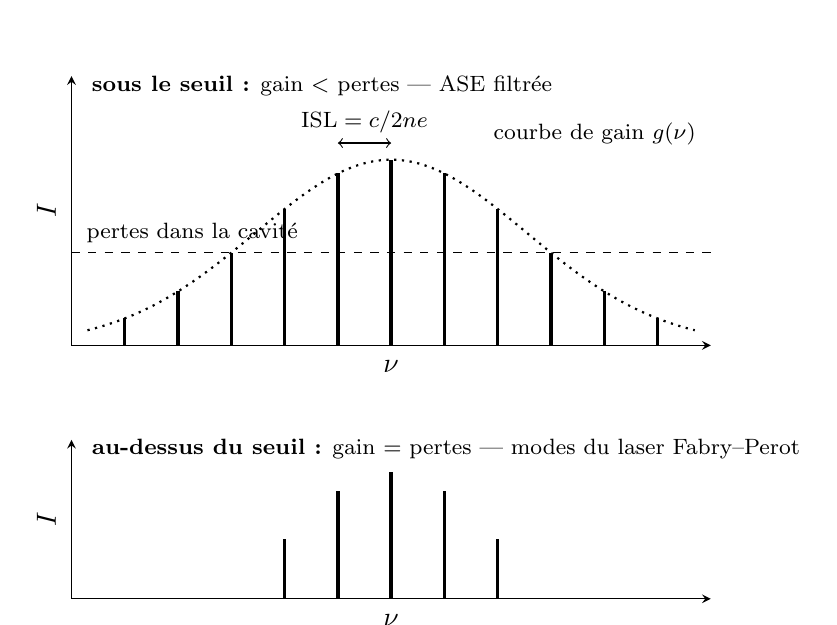
\begin{tikzpicture}
    \begin{axis}[name=top, width=0.8\textwidth, height=5cm,
      xmin=0, xmax=12, ymin=0, ymax=1.45,
      xlabel={$\nu$}, ylabel={$I$}, xtick=\empty, ytick=\empty,
      axis lines=left, clip=false]
      \addplot[black, dotted, thick, domain=0.3:11.7, samples=120]
        {exp(-((x-6)/3.6)^2)};
      \node[font=\footnotesize, anchor=east] at (axis cs:11.9,1.14)
        {courbe de gain $g(\nu)$};
      \addplot[black, dashed, domain=0:12, samples=2] {0.5};
      \node[font=\footnotesize, anchor=south west] at (axis cs:0.1,0.5)
        {pertes dans la cavité};
      \addplot[black, ycomb, very thick] coordinates
        {(1,0.145) (2,0.291) (3,0.499) (4,0.734) (5,0.926) (6,1.0)
         (7,0.926) (8,0.734) (9,0.499) (10,0.291) (11,0.145)};
      \draw[<->] (axis cs:5,1.09) -- (axis cs:6,1.09);
      \node[font=\footnotesize, anchor=south] at (axis cs:5.5,1.09)
        {$\mathrm{ISL}=c/2ne$};
      \node[font=\footnotesize, anchor=west] at (axis cs:0.2,1.40)
        {\textbf{sous le seuil :} gain $<$ pertes --- ASE filtrée};
    \end{axis}
    \begin{axis}[at={(0cm,-1.2cm)}, anchor=north west,
      width=0.8\textwidth, height=3.6cm,
      xmin=0, xmax=12, ymin=0, ymax=1.25,
      xlabel={$\nu$}, ylabel={$I$}, xtick=\empty, ytick=\empty,
      axis lines=left, clip=false]
      \addplot[black, ycomb, very thick] coordinates
        {(4,0.47) (5,0.85) (6,1.0) (7,0.85) (8,0.47)};
      \node[font=\footnotesize, anchor=west] at (axis cs:0.2,1.18)
        {\textbf{au-dessus du seuil :} gain $=$ pertes --- modes du laser Fabry--Perot};
    \end{axis}
  \end{tikzpicture}
  \caption*{\footnotesize Construction of the spectrum of a Fabry--Perot laser.
  Only the modes whose gain compensates the losses survive.}
\end{figure}

Sur la courbe du haut, on peut observer la courbe d'émission spontanée filtrée
par la fonction de transmission de la cavité Fabry--Perot --- la fonction
d'Airy --- dont l'espacement entre les pics est l'intervalle spectral libre
$\mathrm{ISL}=c/2ne$. On peut également observer la valeur des pertes par
aller-retour. La courbe du bas montre le spectre d'émission d'un laser
Fabry--Perot quand le pompage augmente : les pics laser ne sont émis qu'aux
fréquences pour lesquelles le gain est compensé par les pertes : ces pics sont
appelés \textbf{modes longitudinaux du laser}.

\begin{remark}
  Le spectre d'émission d'un laser Fabry--Perot est \emph{a priori multimode}.
  Pour qu'il devienne monomode, il faudrait augmenter les pertes pour les modes
  que l'on souhaite supprimer. Ceci peut être réalisé par exemple à l'aide de
  miroirs sélectifs en longueur d'onde.
\end{remark}

\begin{example}[Switching a laser on]
  The sequence is: allumage du laser, génération de photons spontanés ; si
  photon spontané dans la direction perpendiculaire aux miroirs, amplification
  du photon spontané ; réflexion sur les miroirs ; si longueur d'onde du photon
  spontané pas adaptée à la cavité, interférences destructives, extinction de
  l'onde ; si longueur d'onde du photon spontané adaptée à la cavité,
  l'amplification continue : oscillations.
\end{example}

\subsubsection{Caractéristiques principales d'un faisceau laser}
Les propriétés d'un laser sont très différentes de la lumière « naturelle »
produite par exemple par le soleil ou les lampes à incandescence. Une lampe à
incandescence peut fournir de manière continue une puissance de l'ordre du kW,
dont le spectre en longueur d'onde s'étale sur plusieurs centaines de
nanomètres. Ses longueurs de cohérence spatiale et temporelle sont très
faibles : la longueur de cohérence d'une lumière blanche s'étalant de 0.4 à
0.8 $\mu$m est de l'ordre de 0.8 $\mu$m. De plus, cette lumière n'est pas
polarisée.

\begin{remark}
  On considérera en première approximation que la longueur de cohérence
  correspond à la longueur du train d'onde.
\end{remark}

\paragraph{La monochromaticité de son rayonnement}
La « couleur » de la lumière émise est extrêmement pure, elle correspond à une
onde quasi-sinusoïdale de fréquence située dans le domaine optique
($10^{14}$ Hz). La lumière laser est une association de photons aux propriétés
très voisines --- dans le même état quantique : les photons ne respectent pas le
principe d'exclusion de Pauli --- conséquence intrinsèque de l'émission
stimulée et du filtrage opéré par la cavité. Cette uniformité des photons est
traduite par la notion de \textbf{cohérence temporelle} (\textit{temporal
coherence}) du faisceau, dans laquelle résident toutes les propriétés
remarquables d'une telle source. The longueur de cohérence follows the
linewidth as $L_c=c/\Delta\nu$:

\begin{center}
  \begin{tabular}{lccc}
    \toprule
    $\Delta\nu$ & 1 MHz & 1 kHz & 1 Hz \\
    \midrule
    $L_{\text{coherence}}$ & 300 m & 300 km & 300\,000 km \\
    \bottomrule
  \end{tabular}
\end{center}

\begin{example}
  La longueur de cohérence d'un laser He--Ne de largeur de raie 1.5 GHz est de
  0.2 m et peut atteindre 30 km pour un laser CO$_2$ d'une largeur de raie égale
  à 10 kHz. Notons également plus récemment la réalisation de lasers
  fonctionnant dans le visible (563 nm) et dont la largeur de raie est
  \emph{sub-hertzienne}. Where natural light has a train d'onde a few
  micrometres long, a laser's runs from a few centimetres to a kilometre.
\end{example}

\begin{example}[VIRGO]
  Projet VIRGO : interféromètres pour mesure d'ondes gravitationnelles. Passage
  d'une onde gravitationnelle : déformation d'un milliardième de milliardième de
  mètre dans les bras de 3 km de Virgo --- moins d'un millième de la taille d'un
  proton --- for a source emitting some $3.6\cdot10^{49}$ W. Noise is the whole
  problem, and the measurement is only conceivable with a source of that
  monochromaticity.
\end{example}

\paragraph{La cohérence spatiale de son rayonnement}
Toute la puissance lumineuse peut être concentrée dans un mode de propagation.
C'est ce que l'on appelle la \textbf{cohérence spatiale} (\textit{spatial
coherence}). Le rayonnement laser est focalisable sur de très petites surfaces,
down to the order of $\lambda$. Des densités exceptionnelles de puissance allant
jusqu'à plusieurs mégawatts par mm$^2$ sont possibles.

\begin{remark}
  Being focusable is not the same as being directive. Un faisceau laser n'est
  pas très directif, because of diffraction: a semiconductor laser with an
  emitting zone a few micrometres across diverges by 30 to 60 degrees.
  L'amplification \emph{interne} est très directive, along the cavity axis,
  which is why the amplification is so efficient.
\end{remark}

\paragraph{Des impulsions ultra-courtes}
Localisation temporelle de l'énergie lumineuse : la durée des impulsions de
lumière produites peut être réduite à quelques $10^{-17}$ s (10 attosecondes,
record). Dans ce cas, la source est alors très large spectralement à cause du
principe de Heisenberg. Seuls les lasers continus ont des spectres ultrafins.

\begin{example}
  Laser Mégajoule : durée 20 ns, énergie mégajoule, combinaison de 240
  faisceaux laser fournissant 7.5 kJ chacun --- fusion thermonucléaire. In
  machining, drilling with a femtosecond laser gives a far cleaner hole than a
  nanosecond laser --- la découpe au laser femtoseconde est plus « propre » ---
  which matters for cutting and for surgery of the eye and the brain. Grâce au
  large spectre du continuum d'une source impulsionnelle, on peut même détecter
  plusieurs espèces à la fois (LIDAR), and a Doppler frequency shift gives the
  wind.
\end{example}

\paragraph{Des émissions chaotiques}
A laser can also be driven into a chaotic regime, which is used for private
communications in the mid-infrared, built on photonic chaos with lasers à
cascade quantique in the fenêtre atmosphérique moyen IR, 9--11 $\mu$m.
Pourquoi : rayonnement infrarouge moyen furtif, imprévisibilité du chaos, mise
en œuvre simple. La génération du chaos $C$ est basée sur le signal d'entrée,
donc seul le récepteur qui connaît la façon dont le chaos est généré peut
reproduire le chaos et l'annuler pour récupérer le signal $M$: with a slave
laser regenerating $C'$,
\[M+C-C'=M'\approx M,\qquad C-C'\ll 1,\]
which assumes matched parameters --- or a very small mismatch --- between the two
physical systems, for the chaos to synchronise. Records : 120 km sur fibre
optique et 35 m en espace libre.

\paragraph{La polarisation de son rayonnement}
La nature même de l'émission laser n'oblige pas la lumière laser à être
polarisée. Par contre, il est difficile de supprimer tous les éléments
polarisants dans une cavité. Pour cela, la plupart des lasers sont polarisés
même si en prenant des précautions, on peut faire en sorte qu'ils ne le soient
pas.

\begin{conclusion}[What separates the three emission mechanisms]
  Rayonnement thermique is incoherent, emitted in all directions, over a
  spectre continu several hundred THz wide. Émission spontanée ---
  luminescence --- is also incoherent and emitted in all directions, but it is
  quantised and its spectrum is only a few nanometres wide. Émission stimulée
  clones the incident photon in phase, frequency, direction and polarisation;
  placed in a resonant cavity that filters it and fed by a pompage strong enough
  to invert the populations, it gives a source that is coherent in time and in
  space, monochromatique down to the sub-hertz, and focusable to the longueur
  d'onde.
\end{conclusion}

\section{Holographie}
A photograph records $|A|^2$ and throws the phase away with it.
\textbf{Holographie} (\textit{holography}), found by D. Gabor in 1948, is the
trick that codes the phase of the onde objet into an intensity pattern a
détecteur quadratique can record, and decodes it again by diffraction. What the
eye receives on read-back is the onde the object itself emitted, so the replica
is genuinely three-dimensional: move in front of the plate and the viewing angle
changes.

\subsection{Importance de la phase et de deux yeux pour la vision en 3D}
D'un point de vue humain, nous avons besoin de deux yeux pour voir en volume.
Les deux yeux voient deux angles de vue légèrement différents et le cerveau
reconstitue la vision volumique.

\begin{definition}[Stéréoscopie]
  Principe de la vision volumique de l'être humain : la \textbf{stéréoscopie}
  (\textit{stereoscopy}). Un observateur regardant une scène voit deux images
  similaires mais légèrement décalées de cette scène avec son œil droit et son
  œil gauche ; le cerveau reconstitue 2 images en 2D décalées en une image 3D.
\end{definition}

D'un autre côté, un objet est rendu visible par les ondes lumineuses qu'il émet,
qu'il réfléchit ou qu'il diffuse. Dans le noir un objet est invisible ! Un objet
quelconque peut être considéré comme constitué d'un ensemble de sources
ponctuelles (principe de Huygens-Fresnel), chacune d'entre elles étant
caractérisée par son spectre dont chaque composante a une \textbf{amplitude} et
une \textbf{phase} déterminée, fonction respectivement de la brillance et de la
position relative du point considéré. C'est la raison pour laquelle un objet
éclairé par une lumière peut être observé de différents endroits : chaque point
de l'objet réémet de la lumière dans toutes les directions.\\

Les informations correspondant à l'amplitude et à la phase sont toutes deux
nécessaires à la perception de l'objet et de son relief. Par exemple, dans le
cas d'une onde plane avec une incidence oblique dans le plan $z=0$, s'exprimant
comme :
\[
  A_0(x,y) = a_0(x,y)\,e^{j\varphi_0(x,y)} = a_0(x,y)\,e^{-jkx\sin\theta}.
\]
Si la phase n'est pas enregistrée, on perd l'information sur la direction
$\theta$ de l'onde --- the factor $e^{-jkx\sin\theta}$ is exactly what
disappears.

\begin{remark}
  L'œil, la pellicule argentique (cristaux d'halogénure d'argent --- AgBr, etc.\
  --- qui noircissent sous l'effet de la lumière ; on obtient un négatif qu'il
  faut développer), le capteur CCD ou CMOS : tous ces détecteurs sont
  \textbf{quadratiques}. All of them respond to $|A|^2$ only. Aucun détecteur ne
  peut enregistrer « l'histoire » de l'onde, i.e.\ its phase.
\end{remark}

\begin{conclusion}
  Amplitude \emph{et} phase doivent être enregistrées si l'on désire restituer
  ultérieurement une réplique fidèle de l'objet en trois dimensions et notamment
  si on souhaite rendre compte de tous les angles de vue, condition nécessaire
  pour que chaque œil voie une vue différente de l'autre. Pour résumer, il faut
  trouver un moyen d'enregistrer \emph{tous les angles de vue sur le même
  support} pour que l'on puisse voir d'une part en volume et d'autre part que la
  vue change lorsque l'on se déplace.
\end{conclusion}

\begin{remark}[3D at the cinema]
  La stéréoscopie au cinéma : les anaglyphes, les images polarisées, les images
  alternées (persistance rétinienne). Écrans 3D sans lunettes, ou
  autostéréoscopie : écrans lenticulaires, écrans lenticulaires multivues,
  écrans parallaxes. All of these exploit stéréoscopie and not holographie, and
  they share the same défauts : besoin de lunettes ou position précise devant
  l'écran ; un seul angle de vue ; focalisation sur l'écran alors que l'objet
  est ailleurs --- mal de tête !
\end{remark}

\subsection{Idée de base de l'Holographie}
En photographie classique, il y a deux raisons pour lesquelles on ne voit pas en
3D.

\begin{subpart}
  \item La première est que lors de la formation d'une image avec une lentille,
    chaque point de l'objet n'éclaire qu'un point de l'image. Un seul angle de
    vue est enregistré. On a beau regarder cette image avec les deux yeux, c'est
    comme si elle avait été enregistrée avec un seul. La vision est en 2D : perte
    des angles de vue, perte de profondeur.
  \item Quand bien même on supprimerait la lentille, la phase n'est pas prise en
    compte : l'image est fixée sur une plaque photographique suivant la
    projection 2D de l'intensité de la lumière que l'objet réfléchit. En effet,
    l'émulsion photographique n'est sensible qu'au module au carré du champ : la
    détection est quadratique. Sans lentille, chaque point de l'objet éclaire
    \emph{l'intégralité} de la plaque ; la plaque est alors (quasi) uniformément
    éclairée, il n'y a pas d'image.
\end{subpart}

\begin{figure}[h!]
  \centering
  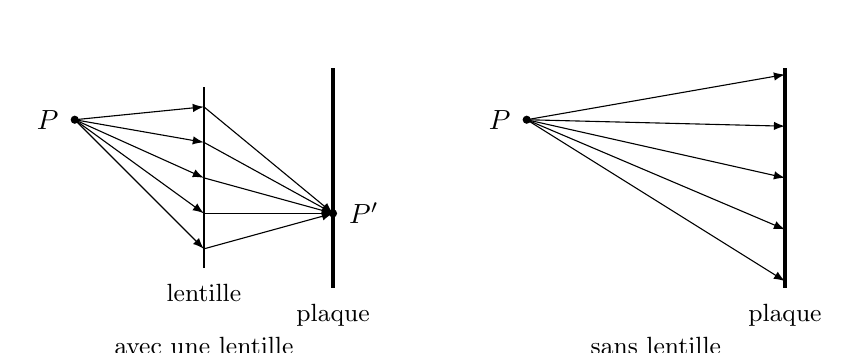
\begin{tikzpicture}[>=latex,scale=0.82]
    % --- with a lens
    \fill (0,0.9) circle (1.8pt); \node[left] at (-0.1,0.9) {$P$};
    \draw[thick] (2,-1.4) -- (2,1.4);
    \node[below] at (2,-1.5) {\small lentille};
    \draw[very thick] (4,-1.7) -- (4,1.7);
    \node[below] at (4,-1.8) {\small plaque};
    \fill (4,-0.55) circle (1.8pt); \node[right] at (4.1,-0.55) {$P'$};
    \foreach \y in {-1.1,-0.55,0,0.55,1.1}{
      \draw[->] (0,0.9) -- (2,\y);
      \draw[->] (2,\y) -- (4,-0.55);
    }
    \node at (2,-2.6) {\small avec une lentille};
    % --- without a lens
    \fill (7,0.9) circle (1.8pt); \node[left] at (6.9,0.9) {$P$};
    \draw[very thick] (11,-1.7) -- (11,1.7);
    \node[below] at (11,-1.8) {\small plaque};
    \foreach \y in {-1.6,-0.8,0,0.8,1.6}{\draw[->] (7,0.9) -- (11,\y);}
    \node at (9,-2.6) {\small sans lentille};
  \end{tikzpicture}
\end{figure}

L'idée de l'holographie est de se donner les moyens d'enregistrer la phase de
l'onde provenant de l'objet. Two conditions follow.

\begin{subpart}
  \item La première condition est de \textbf{supprimer la lentille} pour que
    chaque point de l'objet éclaire l'intégralité de la plaque. Ainsi, chaque
    point de la plaque reçoit l'intégralité de l'information sur l'objet mais vu
    sous un angle donné, c'est-à-dire en 2D. Tous les angles de vue sont
    enregistrés.
  \item La deuxième condition est de trouver un moyen d'enregistrer la phase de
    l'onde objet à l'aide d'un détecteur quadratique puisqu'il n'en existe pas
    d'autres. Pour enregistrer cette phase, \textbf{un code doit être trouvé}
    pour transformer les variations de phase en variations d'intensité.
    L'intensité enregistrée sera ensuite décodée optiquement pour reconstruire
    l'onde initiale. Ce code repose en réalité sur un procédé interférométrique.
    En effet, on sait que si l'on sépare une onde lumineuse en deux faisceaux
    puis qu'on les recombine, l'intensité résultante est une fonction de la
    différence de chemin optique parcouru par les deux ondes (interférences
    constructives ou destructives). C'est un convertisseur de variation de phase
    en variation d'intensité, $\Delta\varphi \to \Delta I$. Il existe donc,
    codée dans la figure d'interférence, une information sur les distances
    relatives des différentes ondes incidentes, donc une information sur le
    volume.
\end{subpart}

\subsection{Éléments de théorie}

\begin{notation}
  The imaginary unit is written $i$ in the general algebra and $j$ in the onde
  plane examples; the two are the same thing. $I_r = |a_r|^2$ et
  $I_0 = |a_0|^2$ sont respectivement les intensités de l'onde de référence et
  de l'onde objet dans le plan $z=0$; $U_0 \equiv A_0$ denotes the onde objet.
  The subscript $r$ is for \textit{référence}, the subscript $0$ for
  \textit{objet}.
\end{notation}

\subsubsection{Enregistrement d'un hologramme}
Le principe du codage holographique est d'enregistrer sur une émulsion
photographique (placée en $z=0$) la figure d'interférences résultant du mélange
entre une onde $A_0$ provenant d'un objet, appelée \textbf{onde objet}
(\textit{object wave}), avec une onde $A_r$ connue, dite \textbf{onde de
référence} (\textit{reference wave}), souvent assimilée à une onde plane. Pour
cela, il faut que les deux ondes soient cohérentes entre elles. L'objet est donc
éclairé par une fraction de l'onde qui sert de référence.

Soit l'expression d'une onde plane choisie comme onde de référence :
\begin{equation*}
  A_r(x,y) = a_r(x,y)\,e^{i\varphi_r(x,y)},
\end{equation*}
avec $|a_r(x,y)|^2$ constant dans le plan de la plaque et $\varphi_r$ dépendant
de l'angle d'incidence :
\begin{equation*}
  \varphi_r(x,y) = \v{k}\cdot\v{r} = k_x x + k_y y + k_z z,
  \qquad \|\v{k}\| = \frac{2\pi}{\lambda},
\end{equation*}
avec $\v{r}$ le vecteur position. Soit l'expression de l'onde objet :
\begin{equation*}
  A_0(x,y) = a_0(x,y)\,e^{i\varphi_0(x,y)},
\end{equation*}
avec $a_0(x,y)$ et $\varphi_0(x,y)$ des expressions compliquées prenant en compte
la somme de l'ensemble des ondes provenant de l'objet. Inutile de détailler ces
deux termes à ce stade. Au point quelconque de coordonnées $(x,y)$, la plaque
reçoit l'amplitude $A_r(x,y)+A_0(x,y)$, et comme l'émulsion photographique n'est
sensible qu'au module au carré du champ,
\begin{equation*}
  I(x,y) \propto |A_r(x,y)+A_0(x,y)|^2
  = |a_r|^2 + |a_0|^2 + a_r^{*}a_0\,e^{-i(\varphi_r-\varphi_0)}
  + a_r a_0^{*}\,e^{i(\varphi_r-\varphi_0)}.
\end{equation*}

\begin{definition}[Hologramme]
  Si la plaque possède, après enregistrement et développement, une transmittance
  $t(x,y)$ \emph{linéairement} proportionnelle à l'intensité enregistrée, alors :
  \begin{equation*}
    \boxed{\;\begin{aligned}
      t(x,y) &\propto |A_r+A_0|^2
      = |a_r|^2+|a_0|^2 + a_r^{*}a_0 e^{-i(\varphi_r-\varphi_0)}
      + a_r a_0^{*}e^{i(\varphi_r-\varphi_0)}\\
      &= I_r + I_0 + 2\sqrt{I_0 I_r}\,
        \cos\!\big[\varphi_r(x,y)-\varphi_0(x,y)\big]
    \end{aligned}\;}
  \end{equation*}
  La transparence obtenue, appelée \textbf{hologramme} (\textit{hologram}),
  contient alors l'information codée sur l'amplitude \emph{et} la phase de $A_0$
  contrairement à une photographie classique --- coded in the cosine term.
\end{definition}

\begin{figure}[h!]
  \centering
  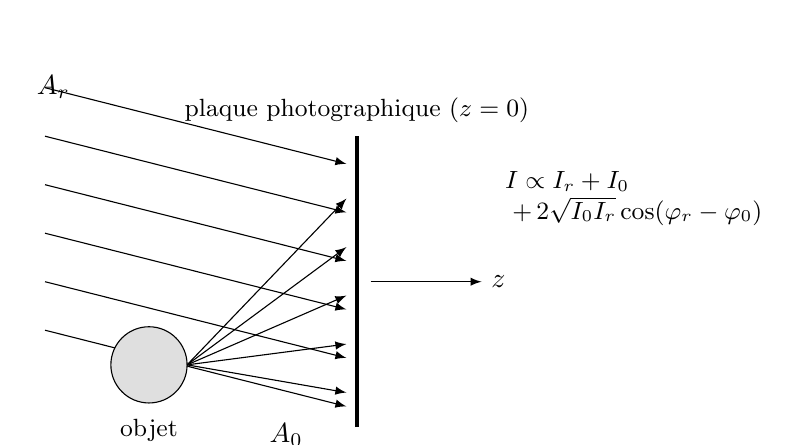
\begin{tikzpicture}[>=latex,scale=0.88]
    \draw[very thick] (3.4,-2.1) -- (3.4,2.1);
    \node[above] at (3.4,2.15) {\small plaque photographique ($z=0$)};
    % reference beam
    \foreach \y in {-1.8,-1.1,-0.4,0.3,1.0,1.7}{\draw[->] (-1.1,\y+1.1) -- (3.25,\y);}
    \node[above left] at (-0.6,2.5) {$A_r$};
    % object
    \draw[fill=gray!25] (0.4,-1.2) circle (0.55);
    \node[below] at (0.4,-1.85) {\small objet};
    \foreach \y in {-1.6,-0.9,-0.2,0.5,1.2}{\draw[->] (0.95,-1.2) -- (3.25,\y);}
    \node[below right] at (2.0,-1.9) {$A_0$};
    \draw[->] (3.6,0) -- (5.2,0) node[right] {$z$};
    \node[right,align=left] at (5.4,1.2)
      {\small $I\propto I_r+I_0$\\[-1pt]\small $\;+\,2\sqrt{I_0I_r}\cos(\varphi_r-\varphi_0)$};
  \end{tikzpicture}
\end{figure}

\subsubsection{Relecture d'un hologramme}
Pour décoder l'information contenue dans l'hologramme et reconstruire l'onde
objet (avec son amplitude et sa phase), l'onde de référence est une nouvelle fois
utilisée pour illuminer l'hologramme. Cette onde va être diffractée par la figure
d'interférence qui est enregistrée sur la plaque. On pourrait étudier en détail
la diffraction de cette onde à distance finie (Fresnel) par l'hologramme mais les
calculs ne sont pas simples. En réalité, il est suffisant d'étudier le champ
transmis \emph{juste après} l'hologramme pour comprendre ce que l'on observe lors
de la relecture. Le résultat est une onde avec une amplitude complexe
$A(x,y) = A_r(x,y)\,t(x,y)$, soit

\begin{theorem}[Les trois ordres de diffraction]
  \begin{align*}
    A(x,y) &= a_r e^{i\varphi_r}\Big[\,|a_r|^2+|a_0|^2
              + a_r^{*}a_0 e^{-i(\varphi_r-\varphi_0)}
              + a_r a_0^{*}e^{i(\varphi_r-\varphi_0)}\Big] \\[2pt]
           &= \underbrace{a_r e^{i\varphi_r}\big(I_r+I_0\big)}_{\text{order }0}
            + \underbrace{|a_r|^2\,U_0}_{\text{order }-1}
            + \underbrace{a_r^2 e^{i2\varphi_r}\,U_0^{*}}_{\text{order }+1}.
  \end{align*}
\end{theorem}

This is the examinable core of the chapter. On distingue dans cette équation
trois termes, appelés \textbf{ordres de diffraction} (\textit{diffraction
orders}), que nous allons détailler --- the three ondes that leave the plate.

\paragraph{Ordre 0 : partie proportionnelle à l'onde de référence.}
\begin{equation*}
  A_{\text{ordre }0} = A_r\,(I_r+I_0).
\end{equation*}
Ce terme représente l'onde de référence modulée par la somme des intensités des
deux ondes initiales. En première approximation, on peut considérer $I_r$ et
$I_0$ uniformes sur la plaque. La direction de $A_{\text{ordre }0}$ est donc
identique à celle de l'onde de référence $A_r$ : il correspond à l'onde de
référence qui traverse l'hologramme sans être diffractée. Il peut être assimilé à
un terme de bruit. En réalité, $I_0$ varie très légèrement sur la plaque suivant
l'objet holographié. Ce terme donne donc lieu à une très faible diffraction de
l'onde plane de référence lors de la reconstruction, que l'on négligera par la
suite ; il peut être appelé « terme ambigu » dans la littérature. Pour négliger
ce terme en pratique, on a coutume également d'augmenter la puissance de l'onde
de référence par rapport à celle de l'onde objet lors de l'écriture.

\paragraph{Ordre $-1$ : partie proportionnelle à l'onde objet.}
\begin{equation*}
  A_{\text{ordre }-1} = |a_r|^2\,U_0 .
\end{equation*}
Ce terme est identique à l'onde objet multipliée par l'intensité de l'onde de
référence. Ce terme reconstitue l'onde objet $A_0$ \emph{en amplitude et en
phase}. On a retrouvé l'objet sous forme d'\textbf{image virtuelle}
(\textit{virtual image}), à l'endroit même où il était lors de l'enregistrement.
L'image restituée est réellement tridimensionnelle : lorsque l'observateur se
déplace devant l'hologramme, l'angle de vue change. On peut décrire l'hologramme
comme une petite fenêtre à travers laquelle on regarderait un objet.

\begin{remark}
  Chaque point de l'objet éclaire l'intégralité de la plaque. Chaque particule
  du matériau photographique contient donc tous les éléments de l'image : elle
  contient l'information de l'ensemble de l'objet mais vu sous un angle donné.
  On peut donc découper un hologramme en plusieurs morceaux et reconstituer avec
  chaque morceau l'image de l'objet entier (en perdant des angles de vue, bien
  sûr).
\end{remark}

\paragraph{Ordre $+1$ : partie proportionnelle à l'onde objet conjuguée.}
\begin{equation*}
  A_{\text{ordre }+1} = a_r^2 e^{i2\varphi_r}\,U_0^{*}.
\end{equation*}
Ce terme, à un facteur d'amplitude près, est l'onde conjuguée de l'onde objet.
C'est une \textbf{image réelle} (\textit{real image}) : elle peut se projeter sur
un écran et même se copier pour dupliquer l'hologramme. Ses profondeurs sont
inversées par rapport à celles de l'objet : l'image réelle est dite
\textbf{pseudoscopique} (\textit{pseudoscopic}) alors que l'image virtuelle est
dite \textbf{orthoscopique} (\textit{orthoscopic}). Le terme de phase
$e^{i2\varphi_r}$ indique la position de l'image réelle ; elle n'est \emph{pas} à
la même position que l'image virtuelle.

\begin{figure}[h!]
  \centering
  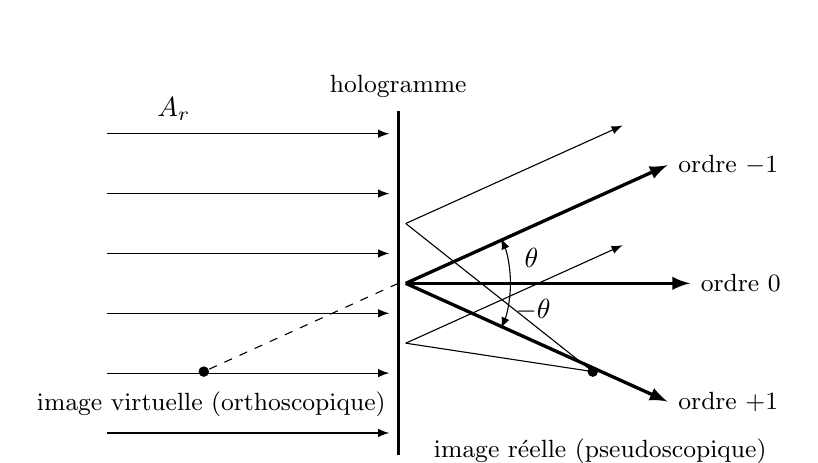
\begin{tikzpicture}[>=latex,scale=0.95]
    \draw[very thick] (0,-2.3) -- (0,2.3);
    \node[above] at (0,2.35) {\small hologramme};
    \foreach \y in {-2.0,-1.2,-0.4,0.4,1.2,2.0}{\draw[->] (-3.9,\y) -- (-0.12,\y);}
    \node[above] at (-3.0,2.05) {$A_r$};
    % order 0
    \draw[->,very thick] (0.1,0) -- (3.9,0) node[right] {\small ordre $0$};
    % order -1
    \draw[->,very thick] (0.1,0) -- (3.6,1.58) node[right] {\small ordre $-1$};
    \draw[->] (0.1,0.8) -- (3.0,2.11);
    \draw[->] (0.1,-0.8) -- (3.0,0.51);
    \draw[dashed] (0,0) -- (-2.6,-1.18);
    \fill (-2.6,-1.18) circle (2pt);
    \node[below] at (-2.5,-1.32) {\small image virtuelle (orthoscopique)};
    % order +1
    \draw[->,very thick] (0.1,0) -- (3.6,-1.58) node[right] {\small ordre $+1$};
    \draw (0.1,0.8) -- (2.6,-1.18);
    \draw (0.1,-0.8) -- (2.6,-1.18);
    \fill (2.6,-1.18) circle (2pt);
    \node[below] at (2.7,-1.95) {\small image réelle (pseudoscopique)};
    \draw[->] (1.5,0) arc (0:23.7:1.5);
    \node at (1.78,0.34) {$\theta$};
    \draw[->] (1.5,0) arc (0:-23.7:1.5);
    \node at (1.80,-0.36) {$-\theta$};
  \end{tikzpicture}
\end{figure}

\begin{remark}[Two sign conventions]
  Two conventions are in use: the ondes written $A = a\,e^{+i\varphi}$, as here,
  or $A(x,y,t) = a\,e^{-i\varphi}e^{i\omega t}$. With the second convention the
  two cross terms swap signs and the three ordres de diffraction read
  $a_r e^{-i\varphi_r}(I_r+I_0) + |a_r|^2 A_0 + a_r^2 e^{-i2\varphi_r}A_0^{*}$.
  The physics is identical; only the sign of every phase exponent changes. Fix
  one convention at the start of a problem and keep it.
\end{remark}

\subsubsection{Hologramme d'une onde plane oblique}
Soit le cas où l'objet est un point lumineux à l'infini. Sur la plaque l'onde
objet est alors une onde plane oblique faisant un angle $\theta$ avec l'axe
$0z$ et une onde de référence plane parallèle à l'axe $0z$
($\varphi_r = 0$). Leur expression peut s'écrire :
\begin{equation*}
  A_r = a_r \qquad\text{and}\qquad A_0 = a_0\,e^{-jkx\sin\theta},
\end{equation*}
où $a_r$ et $a_0$ sont des constantes réelles.

\begin{example}[The three restored waves]
  The general read-back formula gives
  \begin{equation*}
    A(x,y) = \underbrace{a_r\big(I_r+I_0\big)}_{\text{plane wave }\parallel\, 0z}
    \;+\; \underbrace{|a_r|^2 a_0\, e^{-jkx\sin\theta}}_{\text{plane wave at }+\theta}
    \;+\; \underbrace{a_r^2 a_0\, e^{+jkx\sin\theta}}_{\text{plane wave at }-\theta}.
  \end{equation*}
  Le premier terme correspond à une onde plane se propageant dans la direction
  $z$. Le deuxième terme correspond à une onde plane dans la direction $\theta$
  identique à l'onde objet initiale. Le troisième terme correspond à une onde
  plane dans la direction opposée, c'est-à-dire suivant l'angle $-\theta$.
\end{example}

L'onde objet est bien séparée des autres ondes. En fait, cet hologramme est
simplement un enregistrement de franges d'interférences formées par deux ondes
planes se croisant avec un angle $\theta$. Il agit comme un \textbf{réseau de
diffraction sinusoïdal} qui permet de séparer une onde de référence dans trois
directions faisant des angles $0$, $+\theta$ et $-\theta$ par rapport à l'axe
$0z$.

\subsubsection{Hologramme d'un point source à distance finie}
Il est intéressant d'étudier ce cas car tout objet peut être décomposé en une
somme de points sources élémentaires selon le principe de Huygens-Fresnel.
L'hologramme d'un point source peut donc être vu comme l'\textbf{hologramme
élémentaire} (\textit{elementary hologram}). Si l'objet est un point source
situé sur l'axe $0z$ à une distance $-d$ de la plaque holographique, l'onde objet
est une onde sphérique issue du point source dont les coordonnées sont
$\v{r}_0=(0,0,-d)$. L'onde objet peut donc s'exprimer comme :
\begin{equation*}
  A_0(\v{r}) \propto a_0\,\frac{e^{-jk|\v{r}-\v{r}_0|}}{|\v{r}-\v{r}_0|},
  \qquad \v{r}=(x,y,0)\ \text{on the plate}.
\end{equation*}
Une étude détaillée de la figure d'interférence montrerait que l'on obtient une
\textbf{série d'anneaux concentriques}. Term by term:

\begin{subpart}
  \item le premier terme se décompose en une onde plane se propageant dans la
    direction $z$ ainsi qu'un terme proportionnel à $1/|\v{r}-\v{r}_0|^2$ dont
    l'onde se propage dans la direction $z$ avec un angle très petit puisque son
    amplitude varie très lentement dans le plan transverse ;
  \item le deuxième terme est une nouvelle fois similaire à l'onde objet
    initiale : c'est l'\textbf{onde sphérique divergente} qui a été reconstruite.
    Son origine se situe en $(0,0,-d)$, soit exactement la même position que
    celle du point source initial. Cette image est \emph{virtuelle} puisqu'elle
    se forme avant la face de sortie de l'hologramme. Elle ne peut être
    visualisée sur un écran mais peut être imagée par une autre lentille (celle
    de l'œil par exemple) ;
  \item le troisième terme est proportionnel au conjugué de l'onde objet :
    $A_{\text{ordre}+1} \propto a_0\,e^{jk|\v{r}-\v{r}_0|}/|\v{r}-\v{r}_0|$.
    C'est une \textbf{onde sphérique convergente} centrée en $(0,0,+d)$. L'image
    de ce point est donc \emph{réelle} : elle peut être projetée sur un écran.
\end{subpart}

\begin{remark}
  Sur cet exemple, l'onde de référence est parallèle à l'axe $0z$ et le point
  source se trouve sur l'axe. Lors de la restitution, on constate que c'est aussi
  le cas pour l'image conjuguée. On voit qu'il est alors impossible de dissocier
  les différentes images lors de l'observation. Tout est confondu sur l'axe
  $0z$. Note also that the conjugate image of such a hologramme élémentaire
  behaves as a lentille de Fresnel.
\end{remark}

\subsubsection{Holographie hors-axe d'un objet quelconque}
Le moyen de séparer les différentes images est, au moment de l'écriture, de
faire en sorte que l'objet et l'onde de référence ne soient \emph{pas} sur le
même axe optique. On parle alors d'\textbf{holographie hors-axe}
(\textit{off-axis holography}).

Un objet diffusant quelconque peut être considéré comme formé par un grand
nombre de sources ponctuelles d'amplitudes $a_0$ et de phases $\varphi_0$
variables. L'onde diffusée par un objet quelconque peut donc s'exprimer comme :
\begin{equation*}
  f(x,y) = \sum_{\substack{\text{surface}\\ \text{of the object}}} a_0\,e^{j\varphi_0}.
\end{equation*}
Si la direction de cette onde objet fait un angle $\theta$ avec l'axe optique,
c'est une onde dont l'enveloppe complexe $f(x,y)$ portant l'information sur
l'objet est modulée par un facteur de phase qui indique sa direction. The
read-back formula becomes
\begin{equation*}
  A(x,y) \propto a_r e^{i\varphi_r}\Big[I_r + |f(x,y)|^2\Big]
  + |a_r|^2 f(x,y)\,e^{-jkx\sin\theta}
  + a_r^2 f^{*}(x,y)\,e^{+jkx\sin\theta}.
\end{equation*}
Le deuxième terme est une nouvelle fois une réplique de l'onde objet, restituée
avec un angle $\theta$ comme l'indique le terme de phase $e^{-jkx\sin\theta}$.
La présence du facteur $e^{+jkx\sin\theta}$ dans le troisième terme indique que
l'image conjuguée se trouve dans la direction $-\theta$ (par rapport à la
direction de l'onde de référence). Les différentes images restituées sont alors
spatialement séparées et peuvent être observées indépendamment les unes des
autres.

\begin{remark}
  The off-axis onde objet is $A_0(x,y)=f(x,y)e^{-jkx\sin\theta}$, the quantity
  the displayed result uses. Measured from the direction of the onde objet
  rather than from the onde de référence, the conjugate image lies in the
  direction ${\sim}2\theta$ --- the same statement.
\end{remark}

\subsection{Deux familles d'hologrammes : en transmission ou en réflexion}
On a pour habitude d'appeler un hologramme par la manière que l'on utilise pour
le visualiser.

\begin{definition}[Hologrammes en transmission et en réflexion]
  \textbf{Hologramme en transmission} (\textit{transmission hologram}) : on
  regarde le champ transmis par l'hologramme. On place donc lors de la relecture
  son œil de l'autre côté de la plaque --- on the far side from the onde de
  référence.
  \textbf{Hologramme en réflexion} (\textit{reflection hologram}) : on place lors
  de la relecture son œil et l'onde de référence du même côté de la plaque si
  bien que l'on observe les ondes réfléchies par l'hologramme.
\end{definition}

En réalité, ces hologrammes sont très différents. La première différence
concerne la manière dont on enregistre l'hologramme.

\subsubsection{Hologramme en transmission}
Considérons le cas simple où l'onde objet et l'onde de référence sont des ondes
planes cohérentes portées par les vecteurs d'onde $\v{k}_r$ et $\v{k}_0$ à la
longueur d'onde $\lambda_{\text{écriture}}$. Dans le cas d'un hologramme en
transmission, l'objet et l'onde de référence sont placés du \emph{même côté} de
la plaque holographique au moment de l'écriture. L'épaisseur de la gélatine
photographique permettant l'enregistrement s'étend de $z=0$ à $z=\Delta$. Les
franges d'interférences sont alors une fonction des variables $x$, $y$ \emph{et}
$z$ :
\begin{align*}
  I(x,y,z) &\propto \big|a_r e^{-j\v{k}_r\cdot\v{r}} + a_0 e^{-j\v{k}_0\cdot\v{r}}\big|^2\\
           &= I_r+I_0+2\sqrt{I_r I_0}\,\cos\!\big(\v{k}_0\cdot\v{r}-\v{k}_r\cdot\v{r}\big)
            = I_r+I_0+2\sqrt{I_r I_0}\,\cos\!\big(\v{k}_g\cdot\v{r}\big),
\end{align*}
où le vecteur $\v{k}_g = \v{k}_0-\v{k}_r$ est appelé \textbf{vecteur réseau}
(\textit{grating vector}). $I(x,y,z)$ présente des franges d'interférences
sinusoïdales de période $\Lambda = 2\pi/\|\v{k}_g\|$.

Les deux ondes sont cohérentes si bien que
$\|\v{k}_r\|=\|\v{k}_0\|=2\pi/\lambda_{\text{écriture}}$. Les deux vecteurs
faisant un angle $+\theta/2$ et $-\theta/2$ avec l'axe optique, on montre
facilement à l'aide du diagramme des vecteurs que l'expression se simplifie car
$\v{k}_g$ est colinéaire à l'axe $0x$ :
\begin{equation*}
  \v{k}_g\cdot\v{r} = 2\big(\|\v{k}_r\|\sin(\theta/2)\big)x
  = 2\left(\frac{2\pi}{\lambda_{\text{écriture}}}\sin(\theta/2)\right)x,
\end{equation*}
d'où
\begin{equation*}
  I(x,y,z) \propto I_r+I_0+2\sqrt{I_r I_0}\,
  \cos\!\left(2\,\frac{2\pi}{\lambda_{\text{écriture}}}\,x\sin(\theta/2)\right).
\end{equation*}
Les surfaces d'intensité constante (franges d'interférences) sont normales au
vecteur $\v{k}_g$, c'est-à-dire à l'axe $0x$. La période des franges
d'interférence est :
\begin{equation*}
  \boxed{\;\Lambda = \frac{\lambda_{\text{écriture}}}{2\sin(\theta/2)}
  > \frac{\lambda_{\text{écriture}}}{2}.\;}
\end{equation*}
Plus $\theta/2$ augmente, plus $\Lambda$ diminue ; la valeur minimale de
l'interfrange est $\lambda/2$.

\begin{figure}[h!]
  \centering
  \begin{tikzpicture}[>=latex,scale=0.9]
    % --- transmission: emulsion slab, fringes normal to 0x
    \fill[blue!8] (-0.32,-1.5) rectangle (0.32,1.5);
    \draw (-0.32,-1.5) rectangle (0.32,1.5);
    \foreach \y in {-1.2,-0.8,-0.4,0,0.4,0.8,1.2}
      {\draw[red,thick] (-0.32,\y) -- (0.32,\y);}
    \draw[<->] (0.55,0) -- (0.55,0.4); \node[right] at (0.58,0.2) {$\Lambda$};
    \draw[->] (-2.5,1.1) -- (-0.42,0.2); \node[left] at (-2.5,1.1) {$\v{k}_r$};
    \draw[->] (-2.5,-1.1) -- (-0.42,-0.2); \node[left] at (-2.5,-1.1) {$\v{k}_0$};
    \node[align=center] at (-0.7,-2.25)
      {\small en transmission\\[-3pt]\small $\v{k}_g \parallel 0x$, franges $\perp$ surface};
    \draw[->] (-1.5,-3.6) -- (-0.1,-4.05) node[below] {$\v{k}_r$};
    \draw[->] (-1.5,-3.6) -- (-0.1,-3.15) node[above] {$\v{k}_0$};
    \draw[->,very thick] (-0.1,-4.05) -- (-0.1,-3.15);
    \node[right] at (0.0,-3.6) {$\v{k}_g$};
    % --- reflection: fringes parallel to the surface
    \fill[blue!8] (6.08,-1.5) rectangle (6.72,1.5);
    \draw (6.08,-1.5) rectangle (6.72,1.5);
    \foreach \x in {6.16,6.28,6.4,6.52,6.64}
      {\draw[red,thick] (\x,-1.5) -- (\x,1.5);}
    \draw[<->] (6.16,1.72) -- (6.28,1.72); \node[above] at (6.22,1.72) {$\Lambda$};
    \draw[->] (4.1,1.1) -- (5.95,0.35); \node[left] at (4.1,1.1) {$\v{k}_r$};
    \draw[->] (8.7,1.1) -- (6.85,0.35); \node[right] at (8.7,1.1) {$\v{k}_0$};
    \node[align=center] at (6.4,-2.25)
      {\small en réflexion\\[-3pt]\small $\v{k}_g \parallel 0z$, franges $\parallel$ surface};
    \draw[->] (6.4,-3.15) -- (7.6,-3.7) node[right] {$\v{k}_r$};
    \draw[->] (6.4,-3.15) -- (5.2,-3.7) node[left] {$\v{k}_0$};
    \draw[->,very thick] (7.6,-3.7) -- (5.2,-3.7);
    \node[below] at (6.4,-3.78) {$\v{k}_g$};
  \end{tikzpicture}
\end{figure}

Si on enregistre ces franges sur l'émulsion d'épaisseur $\Delta$, ces franges
peuvent être vues comme un réseau de diffraction \emph{épais}. L'hologramme est
appelé \textbf{hologramme de volume} (\textit{volume hologram}). Lorsque ce
réseau est ré-éclairé par une onde plane de longueur d'onde
$\lambda_{\text{relecture}}$ avec le même angle $\theta/2$ que l'onde de
référence initiale, les plans parallèles du réseau de Bragg diffusent la lumière
dans toutes les directions. Dans une direction donnée d'observation $i$, il y a
interférences constructives lorsque la \textbf{condition de Bragg}
(\textit{Bragg condition}) suivante est satisfaite :
\begin{equation*}
  \sin(i) - \sin(\theta/2) = k\,\frac{\lambda_{\text{relecture}}}{\Lambda},
  \qquad k\in\zee .
\end{equation*}

\paragraph{Reconstruction avec une longueur d'onde identique à celle d'écriture.}
Si $\lambda_{\text{relecture}}=\lambda_{\text{écriture}}$, alors, en utilisant
la condition de Bragg et l'expression de $\Lambda$, on montre que :
\begin{equation*}
  \sin(i) = (2k+1)\sin(\theta/2).
\end{equation*}
On constate qu'il existe plusieurs angles (appelés ordres) de diffraction en
fonction de $k$. Pour $k=-1$, $i=\theta/2$ : l'angle de l'ordre $-1$ de
diffraction est égal à l'angle d'incidence de l'onde objet. \emph{L'objet est
reconstitué à la même position que celle initiale de l'objet.} Il existe
d'autres angles où l'on retrouve des répliques de l'objet (other values of
$k$) ; en général, ces répliques sont beaucoup moins intenses.

\paragraph{Reconstruction avec une longueur d'onde différente de celle d'écriture.}
Si $\lambda_{\text{relecture}}\neq\lambda_{\text{écriture}}$, la condition de
Bragg montre cette fois que l'angle de l'ordre $-1$ de diffraction n'est plus
identique à l'angle d'incidence : l'objet ne sera plus au même endroit. On
montre, mais la démonstration n'est pas triviale, que la taille de l'objet est
également modifiée.

\begin{conclusion}
  Un hologramme en transmission sera flou et irisé s'il est éclairé en lumière
  blanche. Un hologramme en transmission doit donc être absolument observé en
  lumière monochromatique. Dans ce cas, si
  $\lambda_{\text{relecture}}\neq\lambda_{\text{écriture}}$, alors la position
  de l'objet restitué change par rapport à sa position initiale mais l'image de
  l'objet reste visible et nette.
\end{conclusion}

\subsubsection{Hologramme en réflexion}
À la différence des hologrammes en transmission, le faisceau de référence et le
faisceau objet sont cette fois placés \emph{de part et d'autre} de la plaque.
L'expression des interférences ne change pas. Par contre, compte tenu des
directions des vecteurs d'onde $\v{k}_r$ et $\v{k}_0$, le vecteur réseau
$\v{k}_g=\v{k}_0-\v{k}_r$ est cette fois parallèle à l'axe $0z$ :
\begin{equation*}
  \v{k}_g\cdot\v{r} = 2\big(\|\v{k}_r\|\cos(\theta/2)\big)z
  = 2\left(\frac{2\pi}{\lambda_{\text{écriture}}}\cos(\theta/2)\right)z,
\end{equation*}
\begin{equation*}
  I(x,y,z) \propto I_r+I_0+2\sqrt{I_r I_0}\,
  \cos\!\left(2\,\frac{2\pi}{\lambda_{\text{écriture}}}\,z\cos(\theta/2)\right).
\end{equation*}
Les franges d'interférences sont \emph{parallèles à la surface} de l'émulsion
photographique (franges dans l'épaisseur). La période des franges d'interférence
devient :
\begin{equation*}
  \boxed{\;\Lambda = \frac{\lambda_{\text{écriture}}}{2\cos(\theta/2)}
  > \frac{\lambda}{2}.\;}
\end{equation*}

Lors de la reconstruction, on ré-illumine l'hologramme avec une onde plane
provenant d'une source blanche et un angle d'incidence $i$ et on regarde le champ
réfléchi par l'hologramme. Son angle de réflexion est identique à l'angle
d'incidence comme nous l'indiquent les lois de Descartes-Snell. Cette onde va
être démultipliée en se réfléchissant sur différents plans d'interférence. On
montre que le déphasage entre une onde réfléchie sous un angle d'incidence $i$
et une autre onde réfléchie qui a traversé une couche supplémentaire est :
\begin{equation*}
  \phi = 2\Lambda\cos(i).
\end{equation*}
On considère qu'une longueur d'onde est réfléchie si le déphasage est un
multiple de $2\pi$. D'après l'expression de l'interfrange $\Lambda$, la longueur
d'onde réfléchie est :
\begin{equation*}
  \boxed{\;\lambda_{\text{réfléchie}}
  = \lambda_{\text{écriture}}\,\frac{\cos(i)}{\cos(\theta/2)}.\;}
\end{equation*}

\begin{conclusion}
  Si l'angle de relecture $i$ est égal à l'angle d'écriture $\theta/2$, la
  longueur d'onde réfléchie sera identique à la longueur d'onde d'écriture. Les
  autres longueurs d'onde ne seront pas réfléchies mais transmises ; ces
  longueurs d'onde ne seront donc pas gênantes. En réflexion, en même temps
  qu'on enregistre un hologramme, on inscrit un filtre appelé \textbf{filtre de
  Bragg} (\textit{Bragg filter}) ou \textbf{miroir de Bragg} (\textit{Bragg
  mirror}) : en réflexion, un hologramme éclairé en lumière blanche sera
  \emph{net et monochrome}. Si au contraire $i \neq \theta/2$, alors
  $\lambda_{\text{réfléchie}} \neq \lambda_{\text{écriture}}$ : lorsqu'on fait
  varier l'angle d'incidence de la lumière blanche, la couleur réfléchie par
  l'hologramme varie mais l'hologramme reste monochrome.
\end{conclusion}

\begin{remark}[Quelques applications des miroirs de Bragg]
  Les miroirs de Bragg sont utilisés dans des domaines de l'optique relativement
  variés comme : traitements antireflets --- lunettes, instruments d'optique
  (télescope, appareil photographique), toutes longueurs d'onde (UV, visible,
  IR) ; lasers --- miroirs haute réflectivité, laser monomode, lasers DFB ou
  VCSEL, affinement de raie laser, lasers à fibre ; fonctions optiques fibrées
  dans les télécommunications --- compensation de dispersion, insertion /
  extraction (Add-Drop) de longueur d'onde dans le réseau. Bien sûr,
  l'empilement des couches peut parfois être très complexe pour obtenir toutes
  sortes de gabarits de filtres.
\end{remark}

\subsection{Contraintes expérimentales}

\subsubsection{Un laser}
Pour enregistrer un hologramme, il faut réaliser des interférences entre une
onde de référence et une onde objet. Cela impose donc de disposer d'une source
cohérente avec un minimum de fluctuations de phase : il faut donc disposer d'un
laser. Le faisceau objet et le faisceau de référence doivent de plus provenir de
la \emph{même} source --- généralement, les deux faisceaux cohérents sont
obtenus en divisant un faisceau laser à l'aide d'une \textbf{lame séparatrice}
(\textit{beam splitter}), par division d'amplitude. On ne peut donc pas
holographier un objet émettant spontanément de la lumière. L'onde objet sera
réalisée par la diffusion d'une onde plane par cet objet, onde cohérente avec
l'onde de référence. La différence de marche entre les deux faisceaux depuis leur
séparation jusqu'à leur recombinaison sur la plaque doit être inférieure à la
longueur de cohérence. Plus la cohérence du laser sera grande, plus le volume des
objets holographiés pourra être grand.

\begin{remark}
  On utilise des lasers à émission continue pour enregistrer des objets
  inanimés. Pour les scènes animées, on utilise des lasers impulsionnels. Une
  impulsion de très forte énergie et d'une durée de l'ordre de la nanoseconde
  permet par exemple de figer une balle à la sortie d'un canon de fusil !
\end{remark}

\subsubsection{Les plaques holographiques}
Une plaque est constituée de grains sensibles à la lumière. Lorsque cette plaque
est plongée dans une solution de révélation, les grains ayant reçu de la lumière
noircissent alors que les autres restent transparents. Three constraints follow.

\paragraph{Taille des grains.}
Puisque les franges d'interférence que l'on souhaite enregistrer sont composées
de fines lignes dont la séparation peut être aussi petite que $\lambda/2$, les
grains de l'émulsion photographique doivent pouvoir discriminer une frange
brillante d'une frange sombre espacées de $\lambda/4$. Leur taille doit donc être
très inférieure à cette valeur. Si le laser d'inscription est un HeNe, la taille
du grain doit alors être très inférieure à $150\,$nm. Les émulsions comportent
donc entre $50\,000$ et $125\,000$ traits/mm (contre
environ $200$ traits/mm pour la photographie classique), soit une taille de grain
qui peut atteindre $8\,$nm contre $5\,\mu$m pour la photographie. En
contrepartie, le film est beaucoup moins sensible et les temps de pose sont de
l'ordre de quelques secondes.

\paragraph{La linéarité de la réponse de la plaque.}
La relation qui nous intéresse est celle qui relie l'amplitude $t$ transmise par
la plaque à l'énergie $W$ reçue par la plaque pendant l'enregistrement. Pour
atteindre la zone de linéarité requise pour enregistrer correctement les franges
d'interférences avec un bon contraste, le temps de pose doit être adapté ---
around the mean received energy $W_0$. En deçà ou au-dessus, le
contraste des franges enregistrées diminue dramatiquement et également en
conséquence l'efficacité de diffraction. L'objet restitué perd en luminosité. Le
choix du temps de pose est donc primordial.

\begin{figure}[h!]
  \centering
  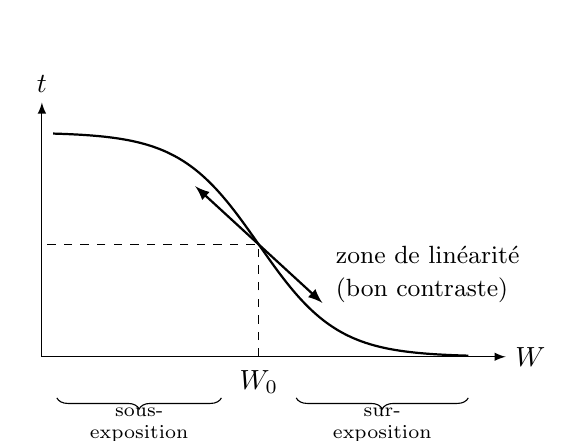
\begin{tikzpicture}[>=latex,scale=0.95]
    \draw[->] (0,0) -- (6.2,0) node[right] {$W$};
    \draw[->] (0,0) -- (0,3.4) node[above] {$t$};
    \draw[thick,domain=0.15:5.7,samples=80,smooth]
      plot (\x,{3/(1+exp(1.9*(\x-2.9)))});
    \draw[dashed] (2.9,0) -- (2.9,1.5) -- (0,1.5);
    \node[below] at (2.9,-0.05) {$W_0$};
    \draw[<->,thick] (2.05,2.28) -- (3.75,0.72);
    \node[right,align=left] at (3.8,1.1) {\small zone de linéarité\\\small (bon contraste)};
    \draw[decorate,decoration={brace,mirror,amplitude=4pt}] (0.2,-0.55) -- (2.4,-0.55)
      node[midway,below,font=\scriptsize,align=center] {sous-\\exposition};
    \draw[decorate,decoration={brace,mirror,amplitude=4pt}] (3.4,-0.55) -- (5.7,-0.55)
      node[midway,below,font=\scriptsize,align=center] {sur-\\exposition};
  \end{tikzpicture}
\end{figure}

\paragraph{Épaisseur des plaques.}
Pour les hologrammes en réflexion, les franges sont parallèles à la surface de
l'hologramme. Pour que le filtre de Bragg soit suffisamment efficace, il faut
enregistrer quelques franges. L'épaisseur de la gélatine doit donc être
supérieure à quelques $\Lambda$, sans quoi il est impossible de réaliser un
hologramme en réflexion. Cette épaisseur n'est pas requise pour les hologrammes
en transmission.

\subsubsection{La stabilité du montage pendant l'inscription}
Puisque l'écart entre une frange brillante et une frange sombre peut être aussi
petit que $\lambda/4$, une vibration peut faire bouger ces franges pendant
l'enregistrement --- la prise de vue peut prendre de quelques secondes à
quelques minutes --- et donc diminuer le contraste des franges enregistrées,
voire les annuler. Il faut donc se donner les moyens de diminuer au maximum les
perturbations extérieures : vibration du montage par le sol, par la ventilation
des appareils, par des bruits acoustiques, vibration de la plaque, mouvement de
l'objet ; variation de température, de pression ou d'hygrométrie ; convection
par le chauffage, par des mouvements dans la pièce, par la chaleur des personnes
ou leur respiration ; gradients thermiques sur la plaque.

\subsubsection{Montage expérimental typique en transmission}
Chaque montage holographique est unique. Il en existe une infinité suivant
l'objet que l'on holographie, l'application, l'angle de vue que l'on souhaite de
l'objet ou de l'onde de référence (qui sera le même en écriture qu'en
relecture). Pour un hologramme en transmission, les règles essentielles à
respecter sont : respect de la cohérence mutuelle des deux ondes ; les deux
ondes doivent être du \emph{même côté} de la plaque. A laser beam is divided on
a lame séparatrice, one arm illuminating the object and the other reaching the
plate directly; at read-back the reference arm alone is restored and the
observer looks through the plate.

\subsubsection{Montage expérimental typique en réflexion : Hologramme de Denisyuk}
Pour un montage en réflexion, les remarques sont les mêmes que pour un
hologramme en transmission si ce n'est que les deux ondes doivent cette fois
arriver \emph{de part et d'autre} de la plaque.

\begin{definition}[Hologramme de Denisyuk]
  L'\textbf{hologramme de Denisyuk} (\textit{Denisyuk hologram}), inventé par
  Y.\,N.\ Denisyuk en 1962, est le montage le plus simple qui soit. C'est un
  hologramme à \emph{faisceau unique} où, au moment de l'écriture, la plaque
  holographique sert elle-même de lame séparatrice. The expanded laser beam
  crosses the plate and plays the part of the onde de référence; the light it
  scatters back off the object, placed just behind the plate, is the onde objet.
\end{definition}

\begin{figure}[h!]
  \centering
  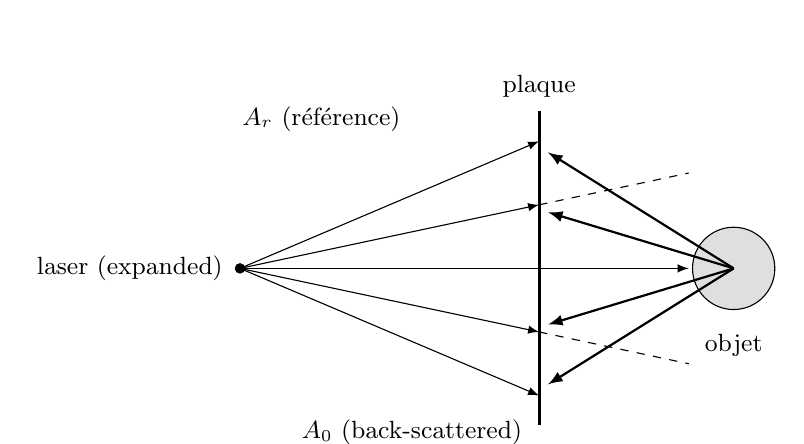
\begin{tikzpicture}[>=latex,scale=0.95]
    \coordinate (S) at (-4.0,0);
    \fill (S) circle (2pt);
    \node[left] at (-4.1,0) {\small laser (expanded)};
    \draw[very thick] (0,-2.1) -- (0,2.1);
    \node[above] at (0,2.15) {\small plaque};
    \foreach \y in {-1.7,-0.85,0.85,1.7}{\draw[->] (S) -- (0,\y);}
    \draw[->] (S) -- (2.0,0);
    \foreach \y in {-0.85,0.85}{\draw[dashed] (0,\y) -- (2.0,{1.5*\y});}
    \draw[fill=gray!25] (2.6,0) circle (0.55);
    \node[below] at (2.6,-0.75) {\small objet};
    \foreach \y in {-1.55,-0.75,0.75,1.55}{\draw[->,thick] (2.6,0) -- (0.12,\y);}
    \node[right] at (-4.1,2.0) {\small $A_r$ (référence)};
    \node[below] at (-1.7,-1.9) {\small $A_0$ (back-scattered)};
  \end{tikzpicture}
\end{figure}

L'hologramme de Denisyuk présente l'avantage d'avoir un réalisme extraordinaire.
Les ombres enregistrées semblent être recréées par la source de référence au
moment de la restitution. Rien de mieux pour tromper l'observateur, même averti !
Il est en plus visible en lumière blanche --- it is a hologramme en réflexion.

\subsection{Applications de l'holographie}
Hormis la réalisation d'images impressionnantes, l'holographie possède
énormément d'applications dans des domaines aussi variés que l'industrie ou la
médecine. L'avènement du numérique dans ce domaine promet un bond en avant
exceptionnel ces prochaines années.

\paragraph{Holographie couleur et muséographie.}
Longtemps inapplicables en muséologie parce qu'ils étaient monochromes et donc
peu réalistes, les hologrammes ont vu leurs domaines d'application s'étendre
depuis la mise au point des hologrammes couleur par Y.\ Gentet, fin des années
90. La difficulté résidait dans l'invention de gélatines sensibles à tout le
spectre visible. Pour rendre compte des couleurs, il suffit alors d'utiliser
trois lasers différents (bleu, vert et rouge) pour enregistrer les hologrammes.
Désormais, dans les musées, certaines œuvres, trop précieuses ou trop fragiles
pour être exposées, sont holographiées avec la plus grande précision. Leurs
images 3D sont alors exposées avec une qualité comparable à l'original.

\paragraph{Photo-inscription et composants optiques.}
Les réseaux de Bragg sont des composants très utilisés dans les réseaux de
télécommunications, notamment dans les commutateurs, les routeurs, les systèmes
de changement ou de décalage spectral. Ils sont utiles pour extraire ou insérer
des longueurs d'onde dans le réseau et compenser la dispersion chromatique. Les
franges de modulation périodique d'indice de réfraction constituant un réseau de
Bragg sont photo-inscrites par laser UV (franges d'interférences UV) dans le
cœur d'une fibre optique monomode (dopage Ge), l'indice du verre étant rendu
dépendant de l'insolation UV qu'il reçoit. Lorsqu'il est ensuite éclairé, ce
réseau se comporte comme un « miroir » pour une bande spectrale très fine autour
d'une longueur d'onde caractéristique (dite « de Bragg »), et transmet toutes les
autres. Dans les technologies DWDM (Dense Wavelength Division Multiplexing), les
informations sont transmises sur une même fibre mais dans des canaux adjacents
caractérisés par des longueurs d'onde différentes. Le réseau de Bragg est un
filtre très sélectif qui ne réfléchit que la longueur d'onde souhaitée. Ainsi,
les multiplexeurs à insertion-extraction peuvent extraire un canal dans le flot
qui arrive à un nœud du réseau puis éventuellement le réinsérer en aval. Les
égalisateurs de gains pour amplificateurs optiques sont également réalisés grâce
à des réseaux de Bragg « longue période » ou « blasés ». Enfin, grâce à des
réseaux à pas variable (dits « chirpés »), on n'a plus seulement une longueur
d'onde concernée par la diffraction mais un continuum de longueurs d'onde, et
cet élargissement du spectre permet d'effectuer de la compensation de
dispersion.

Certains types d'hologrammes agissent sur la lumière mais ne forment pas
d'images 3D : ce sont les \textbf{éléments d'optique holographiques}
(\textit{holographic optical elements}, EOH). Ils consistent à former
l'hologramme d'une optique de base (lentille, lame séparatrice…). L'holographie
permet la création de différents réseaux, dont les densités de traits peuvent
aller de $65$ à plus de $5000$ traits/mm : plans, courbes (concave…), corrigés
des aberrations. Ils sont meilleurs que les réseaux gravés du fait de leur
faible taux d'imperfection. On peut citer la réalisation d'optiques spéciales
pour la focalisation (lentilles holographiques), la séparation ou la déviation
de faisceaux laser, la réalisation de faisceaux pour la spectroscopie, de filtres
d'amplitude et de phase pour la reconnaissance de forme, la correction des
aberrations, l'adressage. Un exemple d'utilisation est la réalisation d'un
tableau de bord composé d'un viseur « tête haute » (HUD, Head Up Display)
comprenant un ou plusieurs miroirs holographiques --- dichroic mirrors. Ces
miroirs sont des hologrammes qui réfléchissent une ou deux couleurs, de largeur
spectrale très faible ; ils sont donc transparents pour quasiment tout le
spectre visible. Un tel miroir permet de donner une image agrandie d'un élément
du tableau de bord; the image is superimposed on the scene. Sur les avions
commerciaux, le HUD sert essentiellement à présenter des informations relatives
à l'environnement telles qu'une piste d'atterrissage masquée par le brouillard.
Augmented-reality headsets use the same idea.

\paragraph{Sécurité et packaging.}
Les hologrammes ne sont quasiment pas copiables. En effet, pour copier un
hologramme, il est nécessaire de faire l'hologramme de l'hologramme, dans des
conditions semblables d'exposition afin de pouvoir respecter la taille et la
forme de l'objet. Cette réalisation étant peu fiable et peu conforme à l'objet
initial, on utilise alors les hologrammes pour certifier la conformité de
certains objets : protection contre les contrefaçons (cartes bancaires,
passeports, cartes d'identité, visas, billets de banque) ; surveillance d'accès
(badges holographiques) ; authentification de produits manufacturés. La plupart
sont de type \textbf{hologrammes arc-en-ciel} (\textit{rainbow holograms}) :
réalisation d'un hologramme par réflexion (master), puis copie de cet hologramme
préalablement recouvert d'une toute petite fente. La profondeur dans l'axe
vertical est sacrifiée. On restitue l'image grâce à la lumière blanche et,
suivant l'angle de vue, l'hologramme change de couleur.

\paragraph{Études de contraintes, détection de défauts.}
Une des applications relativement anciennes de l'holographie est
l'\textbf{interférométrie holographique} (\textit{holographic interferometry}).
Cette technique permet d'étudier les micro-déformations d'un objet diffusant
entre deux expositions avec une extrême précision. On réalise une première
exposition lorsque l'objet est dans une première position, puis une seconde
lorsque l'objet a été déformé (contraintes, variation thermique, etc.). La
différence de trajet parcouru par les ondes dans les deux états de l'objet est
alors rendue visible par une observation des franges d'interférences
superposées à l'objet ; ces franges correspondent aux variations de distance
d'une demi-longueur d'onde. On peut également réaliser cette étude en temps réel
en superposant l'image de l'hologramme et l'objet lui-même. Toute déformation de
l'objet se traduit alors par l'apparition en temps réel de franges
d'interférences. A textbook image shows the vibrations of a guitar body. Les
lignes les plus claires sont les lignes nodales, i.e.\ les endroits où il n'y a
pas de vibration.

\paragraph{Mémoire holographique.}
La mémoire holographique est une technique de mémoire de masse utilisant
l'holographie pour stocker de hautes densités de données dans des cristaux ou
des polymères photosensibles. Elle est souvent désignée comme étant la prochaine
génération de stockage optique des données. En effet, les techniques utilisées
pour les CD ou les DVD atteignent leurs limites physiques (à cause de la taille
de diffraction limitée des rayons d'écriture). L'holographie permet d'utiliser
le \emph{volume} du support au lieu de se limiter à la surface pour enregistrer
des données. De plus, les données peuvent être multiplexées dans le volume
d'enregistrement en ajoutant un angle au faisceau enregistreur par rapport au
faisceau de référence, ou encore en modifiant sa fréquence ou sa phase. Un
faisceau laser est séparé à l'aide d'un cube séparateur en deux faisceaux
respectivement appelés « faisceau de référence » et « faisceau objet ». Pour
l'enregistrement, le faisceau est agrandi par les lentilles afin d'illuminer
complètement un \textbf{modulateur spatial de lumière} (\textit{spatial light
modulator}, SLM) --- en réalité un panneau LCD, ressemblant à une sorte de
grille, où les cases « opaques » et « transparentes » représentent
respectivement les $0$ et les $1$ de l'information à stocker. Le but est de
transférer les données au faisceau objet sous forme d'une page de pixels ; ce
faisceau objet est ensuite focalisé sur le cristal photosensible où il interfère
avec le faisceau de référence (à position angulaire programmable). Le stockage
se fait plan par plan, ce qui permet des débits de données de l'ordre du
Giga-octet par seconde. À la lecture, l'éclairement par le faisceau de référence
(suivant les angles d'enregistrement) conduit à une diffraction de la lumière qui
reconstruit le faisceau objet avec sa page de données ; il ne reste plus qu'à
diriger le faisceau sur la caméra CCD, qui capture instantanément la page
digitale et la décode.

\begin{example}[Orders of magnitude]
  En juin 2006, la société InPhase Technologies annonce la réalisation du
  premier média de stockage holographique : d'une capacité de $300\,$Go, il
  mesure $152\times135\times109\,$mm et atteint un débit de $20\,$Mo/s. Le
  stockage holographique permettrait d'aller jusqu'à $10\,$tera-octets par
  centimètre cube. Pour comparer, pour une carte microSDXC de $256\,$Go la
  densité d'information vaut $1620\,$Go/cm$^3$, pour un disque $2.5''$ de
  $4\,$To la densité vaut $60\,$Go/cm$^3$, pour un disque $3.5''$ de $10\,$To la
  densité vaut $27\,$Go/cm$^3$. Citons également les HVD (Holographic Versatile
  Disc), version holographique du DVD, dont les inventeurs promettent $3.9\,$To,
  soit la capacité de l'équivalent de $830$ DVD ou encore $160$ DVD Blu-ray. Le
  disque HVD fait $12\,$cm de diamètre et $3.5\,$mm d'épaisseur. Ce disque est
  lu par deux rayons laser superposés. Les progrès restant à faire concernent
  les matériaux photosensibles dont il faut encore améliorer la capacité à être
  réinscriptibles, les vitesses d'écriture, la durée de vie.
\end{example}

\begin{remark}
  The Blu-ray equivalent counts single-layer discs:
  $3.9\,$TB $\division 25\,$GB $\approx 156$, hence the $160$; the same capacity
  is also ${\approx}6000$ CD-ROMs.
\end{remark}

\paragraph{Holographie numérique.}
Four variants are distinguished. \emph{Hologramme numérique sur support
analogique} : on crée à l'aide d'un ordinateur la figure d'interférence. L'objet
peut provenir de plusieurs photographies, d'un film panoramique ou même être
généré numériquement. La figure d'interférence est alors imprimée sur un film
holographique, point par point, à l'aide de 3 lasers de 3 couleurs différentes.
Cette technique permet alors de réaliser des hologrammes d'objets vivants.
\emph{Enregistrement d'hologramme sur support numérique} : on peut réaliser
l'expérience en remplaçant la plaque holographique par une matrice de capteur
CCD. On fait ensuite une transformée de Fourier de l'image reçue pour recréer
l'objet informatiquement. Ce principe permettant des diagnostics
tridimensionnels est utilisé dans plusieurs domaines : la médecine, l'industrie.
Exemple : on fait une IRM ou un scanner d'un patient et grâce à un ordinateur on
crée un hologramme de l'organe déficient (utile pour les greffes).
\emph{Projection d'hologramme} : on commence à voir apparaitre des afficheurs
3D, sorte de vidéo-projecteur 3D. \emph{Hologramme tout numérique} : le principe
est de générer un objet numérique (coordonnées de chaque point de l'objet,
brillance), puis, selon les équations de Fresnel, de propager numériquement
chaque onde sphérique provenant de chaque point jusqu'à une plaque virtuelle et
d'en calculer la figure d'interférence avec une onde plane. Cette image est
ensuite envoyée sur un modulateur spatial de lumière puis relue par diffraction.
Un hologramme de cube a été généré numériquement puis reconstitué par
diffraction en couleur à l'aide de trois lasers RVB et trois SLM, à Télécom
Paris.

\begin{remark}
  The fourth variant, the hologramme tout numérique, is genuinely a separate item,
  so four variants are distinguished.
\end{remark}

\paragraph{Limite de résolution actuelle et télévision 3D du futur.}
Of holographie numérique and its SLMs: les limites actuelles résident dans la
taille des pixels qui limitent les angles de vue permis à quelques degrés.
Actuellement, les SLM les plus résolus possèdent des pixels de
$L_{\text{pixel}} = 6\,\mu$m à $8\,\mu$m de large, ce qui permet de discriminer
des franges brillantes ou sombres de $6$ à $8\,\mu$m de large, soit des
interfranges de $12$ à $16\,\mu$m. Or on sait que lorsque deux ondes planes se
croisent, l'interfrange est
\begin{equation*}
  i = \frac{\lambda}{2 n_c \sin\frac{\theta}{2}},
\end{equation*}
on peut donc actuellement enregistrer ou restituer avec ce genre de SLM des
angles de :
\begin{equation*}
  \theta = 2\arcsin\!\left(\frac{\lambda}{2n\times 2L_{\text{pixel}}}\right),
\end{equation*}
soit pour un pixel de $6\,\mu$m, un angle de $2^{\circ}$ seulement.

\begin{remark}
  Equivalently, $\theta_{\max} = 2\arcsin\big(\lambda/2i_{\min}\big)$ with
  $i_{\min}>2d_{\min}$ and $d_{\min}=6\,\mu$m; with another index $n$ and
  longueur d'onde d'écriture the same calculation gives $3^{\circ}$ rather than
  $2^{\circ}$. Either way the order of magnitude is a few degrees.
\end{remark}

Today's 3D television is not holographie at all but stéréoscopie. La technologie
actuelle utilise ce principe en projetant deux films simultanément, pris avec
deux caméras différentes. Ces deux films sont entrelacés sur les lignes de pixels
de l'écran à cristaux liquides et des lunettes spéciales permettent de filtrer
l'une ou l'autre de ces images pour chaque œil. Cependant, ces technologies sont
efficaces pour une position fixe de l'utilisateur mais ne permettent pas de voir
différents angles de vue lorsque l'on se déplace devant l'écran. Les
technologies sans lunette ne lèvent pas ce problème. Une autre technologie peut
potentiellement offrir une 3D plus réaliste : l'holographie digitale. Le front
d'onde objet est recréé à l'aide d'un support à cristaux liquides,
reconfigurables : le SLM. Il permet de recréer le champ complet émis par une
scène, et tous les angles de vue seront enregistrés. The obstacle is exactly the
pixel size. Pour atteindre $60^{\circ}$, il faudrait des pixels d'au maximum
$400\,$nm ; pour atteindre $120^{\circ}$, il faudrait des pixels plus petits que
$200\,$nm. Il faut donc une rupture technologique en trouvant des nouveaux
matériaux capables d'atteindre ces tailles. Verrous à lever : utiliser
des LEDs plutôt que des lasers, augmenter la résolution des SLM --- while
lowering their cost --- et trouver des méthodes de calcul économes pour générer
l'onde objet.

\begin{remark}
  Take a « hologramme » projected onto a stage or a transparent screen --- the
  Pepper's-ghost type of display. Ce n'est pas un hologramme, ce n'est qu'une
  illusion de 3D : no phase has been recorded, and there is no change of viewing
  angle.
\end{remark}

\section{Annexe : tableau de transformées de Fourier}

This table of transformées de Fourier is the one document allowed in the exam, which
is otherwise sat without documents and without a calculator; the table is
supplied. The table below keeps its notation, symbols and sign convention.

\subsection{Variables duales}

\begin{notation}[Espaces duaux]
  The table is written once, in a neutral pair of variables: $\xi$ et $\Xi$
  sont les variables de deux espaces duaux (lettre grecque ksi/xi minuscule et
  majuscule). The transformée de Fourier inverse (left column) and the
  transformée directe (right column) are
  \[
    f(\xi)=\int_{-\infty}^{+\infty}F(\Xi)\exp(2j\pi\xi\Xi)\,d\Xi,
    \qquad
    F(\Xi)=\int_{-\infty}^{+\infty}f(\xi)\exp(-2j\pi\xi\Xi)\,d\xi .
  \]
  The kernel carries $2\pi$ in the exponent, not $\omega$, so there is no
  $1/2\pi$ prefactor anywhere in the table. The engineering $j$ is used, not $i$.
\end{notation}

The table then gives the two substitutions the course actually needs.

\begin{notation}[The two readings of the table]
  \textbf{Temps / fréquences}~:
  \[
    f(t)=\int_{-\infty}^{+\infty}F(\nu)\exp(j2\pi\nu t)\,d\nu
    \qquad\lra\qquad \xi=t \ \text{ and }\ \Xi=\nu .
  \]
  \textbf{Espace / Fréquences spatiales}~:
  \[
    F(x)=\int_{-\infty}^{+\infty}f(u)\exp(-j2\pi ux)\,du
    \qquad\lra\qquad \xi=u \ \text{ and }\ \Xi=x .
  \]
\end{notation}

\begin{remark}
  The two substitutions are not parallel, and this is the commonest way to read
  the table backwards. In the temporal reading the lower-case variable is the
  \emph{signal} variable $t$ and the upper-case one the \emph{frequency} $\nu$.
  In the spatial reading it is the other way round: the lower-case $\xi$ is the
  \emph{fréquence spatiale} $u$ and the upper-case $\Xi$ is the \emph{space}
  variable $x$. So in diffraction the minus-sign integral --- the right-hand
  column --- is the one that carries you from the plane of fréquences spatiales
  back to the object plane, and a pair read left-to-right off the table is a
  $u\to x$ pair, not an $x\to u$ one.
\end{remark}

\subsection{Fonctions d'une seule variable}

\begin{table}[h!]
  \centering
  \begin{tabularx}{\textwidth}{>{\centering\arraybackslash}X >{\centering\arraybackslash}X}
    \toprule
    $\xi$ & $\Xi$ \\
    \midrule
    $\delta(\xi)$ = « delta de Dirac » & $1$ \\[6pt]
    $\delta(\xi-\xi_0)$ & $\exp(-2j\pi\xi_0\Xi)$ \\[6pt]
    $1$ & $\delta(\Xi)$ \\[6pt]
    $\exp(+2j\pi\xi\Xi_0)$ & $\delta(\Xi-\Xi_0)$ \\[6pt]
    $\sin(2\pi\xi\Xi_0)$ &
      $\dfrac{j}{2}\left[\delta(\Xi+\Xi_0)-\delta(\Xi-\Xi_0)\right]$ \\[10pt]
    $\cos(2\pi\xi\Xi_0)$ &
      $\dfrac{1}{2}\left[\delta(\Xi+\Xi_0)+\delta(\Xi-\Xi_0)\right]$ \\
    \bottomrule
  \end{tabularx}
\end{table}

\begin{table}[h!]
  \centering
  \begin{tabularx}{\textwidth}{>{\centering\arraybackslash}X >{\centering\arraybackslash}X}
    \toprule
    $\xi$ & $\Xi$ \\
    \midrule
    $\operatorname{Sign}(\xi)=
      \begin{cases}
        \phantom{-}1 & \text{pour } \xi>0\\
        \phantom{-}0 & \text{pour } \xi=0\\
        -1 & \text{pour } \xi<0
      \end{cases}$
    & $\dfrac{1}{j\pi\Xi}$ \\[16pt]
    $-\dfrac{1}{j\pi\xi}$
    & $\operatorname{Sign}(\Xi)=
      \begin{cases}
        \phantom{-}1 & \text{pour } \Xi>0\\
        \phantom{-}0 & \text{pour } \Xi=0\\
        -1 & \text{pour } \Xi<0
      \end{cases}$ \\[16pt]
    $\operatorname{Step}(\xi)=
      \begin{cases}
        1 & \text{pour } \xi>0\\
        0{,}5 & \text{pour } \xi=0\\
        0 & \text{pour } \xi<0
      \end{cases}$
    & $\dfrac{1}{2}\left[\delta(\Xi)+\dfrac{1}{j\pi\Xi}\right]$ \\[16pt]
    $\dfrac{1}{2}\left[\delta(\xi)-\dfrac{1}{j\pi\xi}\right]$
    & $\operatorname{Step}(\Xi)=
      \begin{cases}
        1 & \text{pour } \Xi>0\\
        0{,}5 & \text{pour } \Xi=0\\
        0 & \text{pour } \Xi<0
      \end{cases}$ \\
    \bottomrule
  \end{tabularx}
\end{table}

\begin{table}[h!]
  \centering
  \begin{tabularx}{\textwidth}{>{\centering\arraybackslash}X >{\centering\arraybackslash}X}
    \toprule
    $\xi$ & $\Xi$ \\
    \midrule
    $\boldsymbol{\omega}_L(\xi)=\displaystyle\sum_{n=-\infty}^{+\infty}\delta(\xi-nL)
      =\frac{1}{L}\sum_{n=-\infty}^{+\infty}\exp\!\left(j\frac{2\pi n\xi}{L}\right)$
    & $\dfrac{1}{L}\,\boldsymbol{\omega}_{1/L}(\Xi)
      =\dfrac{1}{L}\displaystyle\sum_{n=-\infty}^{+\infty}\delta\!\left(\Xi-\frac{n}{L}\right)
      =\sum_{n=-\infty}^{+\infty}\exp(j2\pi nL\Xi)$ \\[22pt]
    $\boldsymbol{\pi}_L(\xi)=\boldsymbol{\pi}\!\left(\dfrac{\xi}{L}\right)=
      \begin{cases}
        1 & \text{si } |\xi|<\dfrac{L}{2}\\[4pt]
        0 & \text{sinon}
      \end{cases}$
    & $L\,\dfrac{\sin \pi\Xi L}{\pi\Xi L}=L\operatorname{Sinc}(\pi\Xi L)$ \\[16pt]
    $L\,\dfrac{\sin \pi\xi L}{\pi\xi L}=L\sinc(\pi\xi L)$
    & $\boldsymbol{\pi}_L(\Xi)=\boldsymbol{\pi}\!\left(\dfrac{\Xi}{L}\right)=
      \begin{cases}
        1 & \text{si } |\Xi|<\dfrac{L}{2}\\[4pt]
        0 & \text{sinon}
      \end{cases}$ \\[16pt]
    $\operatorname{Sinc}^2(\xi)$ & $\operatorname{tri}(\Xi)$ \\[6pt]
    $\operatorname{tri}(\xi)$ & $\operatorname{Sinc}^2(\Xi)$ \\[6pt]
    $\operatorname{Gauss}\!\left(\dfrac{\xi}{L}\right)=\exp\!\left(-\pi\dfrac{\xi^2}{L^2}\right)$
    & $L\operatorname{Gauss}(L\Xi)=L\exp(-\pi L^2\Xi^2)$ \\[12pt]
    $\cos(\pi\xi^2)$ & $\cos\!\left(\pi\left(\Xi^2-\dfrac{1}{4}\right)\right)$ \\[12pt]
    $\sin(\pi\xi^2)$ & $-\sin\!\left(\pi\left(\Xi^2-\dfrac{1}{4}\right)\right)$ \\
    \bottomrule
  \end{tabularx}
\end{table}

\clearpage

\begin{remark}[Reading the table's own function names]
  $\boldsymbol{\pi}$ is the porte of unit height, so
  $\boldsymbol{\pi}_L$ has \emph{total width} $L$ and the condition is
  $|\xi|<L/2$. $\boldsymbol{\omega}_L$ is the peigne de Dirac of period $L$,
  poids $1$. $\operatorname{tri}$ is
  the unit triangle. $\operatorname{Gauss}$ is normalised so that
  $\operatorname{Gauss}(0)=1$ and the $\pi$ sits in the exponent, which is
  exactly what makes the Gaussian its own transform up to the $L$ scaling.
\end{remark}

\begin{remark}[The table uses two different $\sinc$ conventions]
  In the porte rows the table spells the meaning out,
  $L\,\frac{\sin\pi\xi L}{\pi\xi L}=L\sinc(\pi\xi L)$, so there
  $\sinc(x)=\sin x/x$ and the $\pi$ is already written into the argument;
  feeding such a row an argument without the $\pi$ is the fastest way to lose a
  factor of $\pi$ in a diffraction calculation. The
  $\operatorname{Sinc}^2\lra\operatorname{tri}$ rows, by contrast, are printed
  with no $\pi$ anywhere in the argument and are correct only for the
  \emph{normalised} $\operatorname{Sinc}(x)=\sin(\pi x)/(\pi x)$: read them the
  unnormalised way and $\left(\frac{\sin\xi}{\xi}\right)^2$ transforms to
  $\pi\operatorname{tri}(\pi\Xi)$, not $\operatorname{tri}(\Xi)$. The table
  gives both conventions the same name (spelt $L\,sinc$ in one row and
  $L\,Sinc$ or $\operatorname{Sinc}^2$ elsewhere; the capitalisation carries no
  meaning), so read each row by whether the $\pi$ is written.
\end{remark}

\begin{remark}[Le poids du peigne]
  The transform of a peigne de Dirac of period $L$ and unit poids is a peigne of
  period $1/L$ carrying poids $1/L$, not $1$. The second equality in each cell
  is the Poisson summation identity; it is the entry the sampling arguments of the
  diffraction chapter rest on, and the $1/L$ is the part most often dropped.
\end{remark}

\begin{figure}[h!]
  \centering
  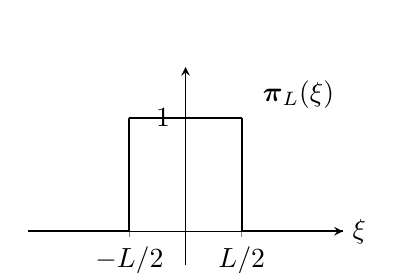
\begin{tikzpicture}
    \begin{axis}[
      width=0.46\textwidth, height=4.1cm,
      axis lines=middle, xlabel={$\xi$},
      xtick={-1,1}, xticklabels={$-L/2$,$L/2$},
      ytick={1}, yticklabels={$1$},
      xmin=-2.8, xmax=2.8, ymin=-0.3, ymax=1.45,
      every axis x label/.style={at={(ticklabel* cs:1.0)},anchor=west},
      ]
      \addplot[thick,domain=-2.8:-1,samples=2]{0};
      \addplot[thick,domain=-1:1,samples=2]{1};
      \addplot[thick,domain=1:2.8,samples=2]{0};
      \draw[thick] (axis cs:-1,0) -- (axis cs:-1,1);
      \draw[thick] (axis cs:1,1) -- (axis cs:1,0);
      \node[anchor=south west] at (axis cs:1.2,1.0) {$\boldsymbol{\pi}_L(\xi)$};
    \end{axis}
  \end{tikzpicture}
  \hfill
  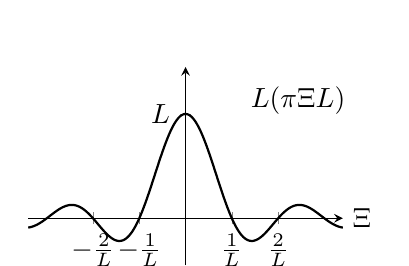
\begin{tikzpicture}
    \begin{axis}[
      width=0.46\textwidth, height=4.1cm,
      axis lines=middle, xlabel={$\Xi$},
      xtick={-2,-1,1,2}, xticklabels={$-\frac{2}{L}$,$-\frac{1}{L}$,$\frac{1}{L}$,$\frac{2}{L}$},
      ytick={1}, yticklabels={$L$},
      xmin=-3.4, xmax=3.4, ymin=-0.45, ymax=1.45,
      every axis x label/.style={at={(ticklabel* cs:1.0)},anchor=west},
      ]
      \addplot[thick,domain=-3.4:3.4,samples=200]{sin(deg(pi*x))/(pi*x)};
      \node[anchor=south west] at (axis cs:1.2,0.9) {$L\sinc(\pi\Xi L)$};
    \end{axis}
  \end{tikzpicture}
  \caption*{}
\end{figure}

\begin{figure}[h!]
  \centering
  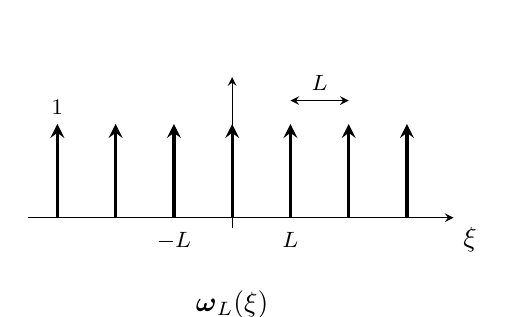
\begin{tikzpicture}[>=stealth, xscale=0.74, yscale=0.85]
    \draw[->] (-3.5,0) -- (3.8,0) node[below right] {$\xi$};
    \draw[->] (0,-0.15) -- (0,2.1);
    \foreach \x in {-3,-2,-1,0,1,2,3} \draw[->,very thick] (\x,0) -- (\x,1.4);
    \draw[<->] (1,1.75) -- (2,1.75) node[midway,above] {\footnotesize $L$};
    \node[anchor=south] at (-3,1.4) {\footnotesize $1$};
    \node[anchor=north] at (1,-0.08) {\footnotesize $L$};
    \node[anchor=north] at (-1,-0.08) {\footnotesize $-L$};
    \node at (0,-1.3) {$\boldsymbol{\omega}_L(\xi)$};
  \end{tikzpicture}
  \hspace{0.015\textwidth}
  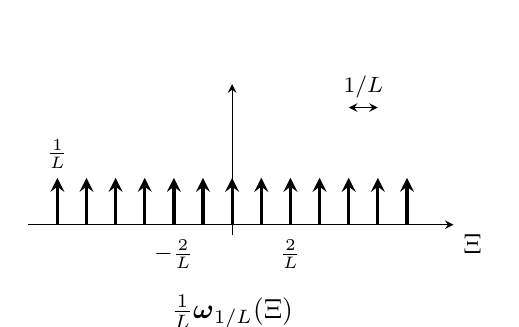
\begin{tikzpicture}[>=stealth, xscale=0.74, yscale=0.85]
    \draw[->] (-3.5,0) -- (3.8,0) node[below right] {$\Xi$};
    \draw[->] (0,-0.15) -- (0,2.1);
    \foreach \x in {-3,-2.5,-2,-1.5,-1,-0.5,0,0.5,1,1.5,2,2.5,3}
      \draw[->,very thick] (\x,0) -- (\x,0.7);
    \draw[<->] (2,1.75) -- (2.5,1.75) node[midway,above] {\footnotesize $1/L$};
    \node[anchor=south] at (-3,0.7) {\footnotesize $\tfrac{1}{L}$};
    \node[anchor=north] at (1,-0.08) {\footnotesize $\tfrac{2}{L}$};
    \node[anchor=north] at (-1,-0.08) {\footnotesize $-\tfrac{2}{L}$};
    \node at (0,-1.3) {$\tfrac{1}{L}\boldsymbol{\omega}_{1/L}(\Xi)$};
  \end{tikzpicture}
  \caption*{}
\end{figure}

\subsection{Fonctions de deux variables}

Ce tableau s'applique pour le cas de la diffraction, c'est-à-dire de l'espace
$(x,y)$ à l'espace des fréquences spatiales $(u,v)$.

\begin{table}[h!]
  \centering
  \begin{tabularx}{\textwidth}{>{\centering\arraybackslash}X >{\centering\arraybackslash}X}
    \toprule
    $\displaystyle f(\v{\rho})=\int_{-\infty}^{+\infty}F(\v{r})\exp(2j\pi \v{r}\v{\rho})\,d^2\v{r}$
      \newline \textit{Avec} $\v{\rho}(u,v)$
    & $\displaystyle F(\v{r})=\int_{-\infty}^{+\infty}f(\v{\rho})\exp(-2j\pi \v{r}\v{\rho})\,d^2\v{\rho}$
      \newline \textit{Avec} $\v{r}(x,y)$ \\
    \midrule
    $f(u)\,g(v)$
    & $F(x)\,G(y)$ \newline \textit{fonction à variables séparables} \\[8pt]
    $1(u)\,1(v)$ & $\delta(x,y)$ \\[8pt]
    $\dfrac{\pi D^2}{4}\operatorname{Somb}(\rho D)
      =\dfrac{\pi D^2}{4}\,\dfrac{2J_1(\pi\rho D)}{\pi\rho D}$
    & $\operatorname{Circ}\!\left(\dfrac{r}{D}\right)=
      \begin{cases}
        1 & \text{pour } r\le \dfrac{D}{2}\\[6pt]
        0 & \text{pour } r\ge \dfrac{D}{2}
      \end{cases}$ \\[20pt]
    $r_0^2\operatorname{Gauss}(\rho r_0)=r_0^2\exp(-\pi r_0^2\rho^2)$
    & $\operatorname{Gauss}\!\left(\dfrac{r}{r_0}\right)
      =\exp\!\left(-\pi\dfrac{r^2}{r_0^2}\right)$ \\
    \bottomrule
  \end{tabularx}
\end{table}

\begin{remark}[The second table's variables and its Bessel function]
  The right-hand column's variable is $\v{r}(x,y)$: the whole point of the
  second table is that $\v{\rho}$ lives in the plane of fréquences spatiales
  $(u,v)$ and $\v{r}$ in the object plane $(x,y)$, as the rows
  $f(u)g(v)\lra F(x)G(y)$ and $\operatorname{Circ}(r/D)$ make plain.\\

  The $\operatorname{Somb}$ entry carries $J_1$, the fonction de Bessel de
  première espèce of order one, and not $J_0$. With $J_0$ the expression would
  diverge at $\rho=0$, since $J_0(0)=1$ and the $\pi\rho D$ in the denominator
  vanishes, whereas the value at the origin must be the aperture area
  $\pi D^2/4$. Only $2J_1(x)/x\to 1$ as $x\to 0$ does that, and it is $J_1$
  whose first zero at $x=1{,}22\pi$ gives the Airy radius.
\end{remark}

\begin{remark}
  $\operatorname{Circ}(r/D)$ is written in terms of the \emph{diameter} $D$, not
  the radius, so its support is $r\le D/2$ and its area is $\pi D^2/4$ --- which
  is the prefactor in front of $\operatorname{Somb}$, as it must be. Likewise
  $\operatorname{Gauss}(r/r_0)$ uses the $1/e$-of-$\pi$ radius $r_0$, and the
  transform picks up $r_0^2$, one power of $r_0$ per dimension, against the
  single power of $L$ in the one-variable table.
\end{remark}

\subsection{Autres paires à deux dimensions}

Four further two-dimensional pairs complete the table. They do not follow the
notation of the tables above: the peigne is written $\mathrm{III}$ rather than
$\boldsymbol{\omega}$, the imaginary unit is $i$ rather than $j$, and the
two-dimensional Dirac is $\delta^2(x,y)$ rather than $\delta(x,y)$.

\begin{table}[h!]
  \centering
  \begin{tabularx}{\textwidth}{>{\centering\arraybackslash}X >{\centering\arraybackslash}X}
    \toprule
    $(x,y)$ & $(u,v)$ \\
    \midrule
    $\delta^2(x,y)$ & $1$ \\[6pt]
    $\mathrm{III}(y)\,\delta(x)$ & $\mathrm{III}(v)$ \\[6pt]
    $\exp\!\left(-\pi\dfrac{x^2+y^2}{a^2}\right)$ & $a^2\exp\!\left(-\pi a^2(u^2+v^2)\right)$ \\[12pt]
    $\sin \pi y$
    & $\dfrac{i}{2}\,\delta^2\!\left(u,v-\dfrac{1}{2}\right)
      -\dfrac{i}{2}\,\delta^2\!\left(u,v+\dfrac{1}{2}\right)$ \\
    \bottomrule
  \end{tabularx}
\end{table}

\begin{remark}[These pairs use the opposite sign convention]
  The last row contradicts the one-variable table. With the table's kernel
  $\exp(-2j\pi\xi\Xi)$, the entry $\sin(2\pi\xi\Xi_0)\lra
  \frac{j}{2}\left[\delta(\Xi+\Xi_0)-\delta(\Xi-\Xi_0)\right]$ applied to
  $\sin\pi y=\sin(2\pi\cdot\tfrac12\cdot y)$ gives
  $\frac{j}{2}\left[\delta(v+\tfrac12)-\delta(v-\tfrac12)\right]$ --- the
  opposite sign to the last row, which is written with the conjugate kernel
  $\exp(+2i\pi)$. Use the one-variable table's sign, since that is the one the
  rest of the course and the exam follow.\\

  The Gaussian row's transform is $a^2\exp(-\pi a^2(u^2+v^2))$, with one power
  of $a$ per dimension, like the $r_0^2$ of the two-variable table above.
\end{remark}

\subsection{Ce que le tableau ne donne pas}

\begin{remark}
  The table is a table of \emph{pairs} only. It carries no properties or
  theorems section: linéarité, changement d'échelle, translation ou déphasage
  and the théorème de Parseval-Plancherel belong to chapter 2 and are \emph{not} handed out. Neither is the théorème de
  convolution. Those have to be carried into the room in your head; only the
  pairs above are on the desk.
\end{remark}

A short bibliography for the course: L. Léger, \textit{Cours d'optique
géométrique et ondulatoire} (Orsay, 1992); B. Saleh and
M. Teich, \textit{Fundamentals of Photonics} (Wiley, 1991); I. and M. Joindot,
\textit{Les télécommunications par fibres optiques} (Dunod, 1996); J.-P. Pérez,
\textit{Optique géométrique et ondulatoire} (Masson, 1994); G. M. Stéphan,
\textit{Cours d'optique de Fourier} (Rennes, 1996).

\end{document}
